% Options for packages loaded elsewhere
% Options for packages loaded elsewhere
\PassOptionsToPackage{unicode}{hyperref}
\PassOptionsToPackage{hyphens}{url}
\PassOptionsToPackage{dvipsnames,svgnames,x11names}{xcolor}
%
\documentclass[
  spanish,
  a4paper,
  12pt,
  twoside]{memoir}
\usepackage{xcolor}
\usepackage{amsmath,amssymb}
\setcounter{secnumdepth}{5}
\usepackage{iftex}
\ifPDFTeX
  \usepackage[T1]{fontenc}
  \usepackage[utf8]{inputenc}
  \usepackage{textcomp} % provide euro and other symbols
\else % if luatex or xetex
  \usepackage{unicode-math} % this also loads fontspec
  \defaultfontfeatures{Scale=MatchLowercase}
  \defaultfontfeatures[\rmfamily]{Ligatures=TeX,Scale=1}
\fi
\usepackage{lmodern}
\ifPDFTeX\else
  % xetex/luatex font selection
\fi
% Use upquote if available, for straight quotes in verbatim environments
\IfFileExists{upquote.sty}{\usepackage{upquote}}{}
\IfFileExists{microtype.sty}{% use microtype if available
  \usepackage[]{microtype}
  \UseMicrotypeSet[protrusion]{basicmath} % disable protrusion for tt fonts
}{}
\makeatletter
\@ifundefined{KOMAClassName}{% if non-KOMA class
  \IfFileExists{parskip.sty}{%
    \usepackage{parskip}
  }{% else
    \setlength{\parindent}{0pt}
    \setlength{\parskip}{6pt plus 2pt minus 1pt}}
}{% if KOMA class
  \KOMAoptions{parskip=half}}
\makeatother
% Make \paragraph and \subparagraph free-standing
\makeatletter
\ifx\paragraph\undefined\else
  \let\oldparagraph\paragraph
  \renewcommand{\paragraph}{
    \@ifstar
      \xxxParagraphStar
      \xxxParagraphNoStar
  }
  \newcommand{\xxxParagraphStar}[1]{\oldparagraph*{#1}\mbox{}}
  \newcommand{\xxxParagraphNoStar}[1]{\oldparagraph{#1}\mbox{}}
\fi
\ifx\subparagraph\undefined\else
  \let\oldsubparagraph\subparagraph
  \renewcommand{\subparagraph}{
    \@ifstar
      \xxxSubParagraphStar
      \xxxSubParagraphNoStar
  }
  \newcommand{\xxxSubParagraphStar}[1]{\oldsubparagraph*{#1}\mbox{}}
  \newcommand{\xxxSubParagraphNoStar}[1]{\oldsubparagraph{#1}\mbox{}}
\fi
\makeatother

\usepackage{color}
\usepackage{fancyvrb}
\newcommand{\VerbBar}{|}
\newcommand{\VERB}{\Verb[commandchars=\\\{\}]}
\DefineVerbatimEnvironment{Highlighting}{Verbatim}{commandchars=\\\{\}}
% Add ',fontsize=\small' for more characters per line
\usepackage{framed}
\definecolor{shadecolor}{RGB}{241,243,245}
\newenvironment{Shaded}{\begin{snugshade}}{\end{snugshade}}
\newcommand{\AlertTok}[1]{\textcolor[rgb]{0.68,0.00,0.00}{#1}}
\newcommand{\AnnotationTok}[1]{\textcolor[rgb]{0.37,0.37,0.37}{#1}}
\newcommand{\AttributeTok}[1]{\textcolor[rgb]{0.40,0.45,0.13}{#1}}
\newcommand{\BaseNTok}[1]{\textcolor[rgb]{0.68,0.00,0.00}{#1}}
\newcommand{\BuiltInTok}[1]{\textcolor[rgb]{0.00,0.23,0.31}{#1}}
\newcommand{\CharTok}[1]{\textcolor[rgb]{0.13,0.47,0.30}{#1}}
\newcommand{\CommentTok}[1]{\textcolor[rgb]{0.37,0.37,0.37}{#1}}
\newcommand{\CommentVarTok}[1]{\textcolor[rgb]{0.37,0.37,0.37}{\textit{#1}}}
\newcommand{\ConstantTok}[1]{\textcolor[rgb]{0.56,0.35,0.01}{#1}}
\newcommand{\ControlFlowTok}[1]{\textcolor[rgb]{0.00,0.23,0.31}{\textbf{#1}}}
\newcommand{\DataTypeTok}[1]{\textcolor[rgb]{0.68,0.00,0.00}{#1}}
\newcommand{\DecValTok}[1]{\textcolor[rgb]{0.68,0.00,0.00}{#1}}
\newcommand{\DocumentationTok}[1]{\textcolor[rgb]{0.37,0.37,0.37}{\textit{#1}}}
\newcommand{\ErrorTok}[1]{\textcolor[rgb]{0.68,0.00,0.00}{#1}}
\newcommand{\ExtensionTok}[1]{\textcolor[rgb]{0.00,0.23,0.31}{#1}}
\newcommand{\FloatTok}[1]{\textcolor[rgb]{0.68,0.00,0.00}{#1}}
\newcommand{\FunctionTok}[1]{\textcolor[rgb]{0.28,0.35,0.67}{#1}}
\newcommand{\ImportTok}[1]{\textcolor[rgb]{0.00,0.46,0.62}{#1}}
\newcommand{\InformationTok}[1]{\textcolor[rgb]{0.37,0.37,0.37}{#1}}
\newcommand{\KeywordTok}[1]{\textcolor[rgb]{0.00,0.23,0.31}{\textbf{#1}}}
\newcommand{\NormalTok}[1]{\textcolor[rgb]{0.00,0.23,0.31}{#1}}
\newcommand{\OperatorTok}[1]{\textcolor[rgb]{0.37,0.37,0.37}{#1}}
\newcommand{\OtherTok}[1]{\textcolor[rgb]{0.00,0.23,0.31}{#1}}
\newcommand{\PreprocessorTok}[1]{\textcolor[rgb]{0.68,0.00,0.00}{#1}}
\newcommand{\RegionMarkerTok}[1]{\textcolor[rgb]{0.00,0.23,0.31}{#1}}
\newcommand{\SpecialCharTok}[1]{\textcolor[rgb]{0.37,0.37,0.37}{#1}}
\newcommand{\SpecialStringTok}[1]{\textcolor[rgb]{0.13,0.47,0.30}{#1}}
\newcommand{\StringTok}[1]{\textcolor[rgb]{0.13,0.47,0.30}{#1}}
\newcommand{\VariableTok}[1]{\textcolor[rgb]{0.07,0.07,0.07}{#1}}
\newcommand{\VerbatimStringTok}[1]{\textcolor[rgb]{0.13,0.47,0.30}{#1}}
\newcommand{\WarningTok}[1]{\textcolor[rgb]{0.37,0.37,0.37}{\textit{#1}}}

\usepackage{longtable,booktabs,array}
\newcounter{none} % for unnumbered tables
\usepackage{calc} % for calculating minipage widths
% Correct order of tables after \paragraph or \subparagraph
\usepackage{etoolbox}
\makeatletter
\patchcmd\longtable{\par}{\if@noskipsec\mbox{}\fi\par}{}{}
\makeatother
% Allow footnotes in longtable head/foot
\IfFileExists{footnotehyper.sty}{\usepackage{footnotehyper}}{\usepackage{footnote}}
\makesavenoteenv{longtable}
\usepackage{graphicx}
\makeatletter
\newsavebox\pandoc@box
\newcommand*\pandocbounded[1]{% scales image to fit in text height/width
  \sbox\pandoc@box{#1}%
  \Gscale@div\@tempa{\textheight}{\dimexpr\ht\pandoc@box+\dp\pandoc@box\relax}%
  \Gscale@div\@tempb{\linewidth}{\wd\pandoc@box}%
  \ifdim\@tempb\p@<\@tempa\p@\let\@tempa\@tempb\fi% select the smaller of both
  \ifdim\@tempa\p@<\p@\scalebox{\@tempa}{\usebox\pandoc@box}%
  \else\usebox{\pandoc@box}%
  \fi%
}
% Set default figure placement to htbp
\def\fps@figure{htbp}
\makeatother



\ifLuaTeX
\usepackage[bidi=basic,shorthands=off]{babel}
\else
\usepackage[bidi=default,shorthands=off]{babel}
\fi
\ifLuaTeX
  \usepackage{selnolig} % disable illegal ligatures
\fi


\setlength{\emergencystretch}{3em} % prevent overfull lines

\providecommand{\tightlist}{%
  \setlength{\itemsep}{0pt}\setlength{\parskip}{0pt}}



 
\usepackage[]{natbib}
\bibliographystyle{apalike}


%% ============================================================
%%  Preámbulo LaTeX – Anexos TFG GIS UBU
%%  Mismo contenido que preambulo_memoria.tex; se mantiene
%%  separado para facilitar ajustes independientes.
%% ============================================================

%\usepackage[spanish,es-tabla]{babel} % No es necesario en Quarto
%\selectlanguage{spanish} % No es necesario en Quarto
\addto\captionsspanish{\renewcommand{\tablename}{Tabla}}
\addto\captionsspanish{\renewcommand{\listtablename}{Índice de tablas}}
\addto\captionsspanish{\renewcommand{\contentsname}{Índice general}}
\addto\captionsspanish{\renewcommand{\listfigurename}{Índice de figuras}}


\usepackage{lmodern}
\usepackage{microtype}
\usepackage{placeins}

\RequirePackage{booktabs}
%\RequirePackage[table]{xcolor}
\PassOptionsToPackage{table}{xcolor}
\RequirePackage{xtab}
\RequirePackage{multirow}
\RequirePackage{tabularx}

\PassOptionsToPackage{hyphens}{url}
\usepackage[colorlinks]{hyperref}
\hypersetup{allcolors={red}}

\usepackage{amsmath}

\nonzeroparskip
\widowpenalty100000
\clubpenalty100000
\nouppercaseheads

\let\tmp\oddsidemargin
\let\oddsidemargin\evensidemargin
\let\evensidemargin\tmp
\reversemarginpar

\usepackage{graphicx}
\graphicspath{{./img/}}

\newcommand{\imagen}[3]{%
  \begin{figure}[!h]
    \centering
    \includegraphics[width=#3\textwidth]{#1}
    \caption{#2}\label{fig:#1}
  \end{figure}
  \FloatBarrier
}

\newcommand{\ruta}[1]{{\sffamily #1}}

\chapterstyle{bianchi}

%% Para los anexos NO se usa \capitulo; se usa \apendice
\renewcommand{\appendixname}{Apéndice}
\renewcommand*\cftappendixname{\appendixname}
\newcommand{\apendice}[1]{\chapter{#1}}
\renewcommand*\cftappendixname{\appendixname\ }

\usepackage{xcolor}
\definecolor{newBox}{HTML}{D8AD6E}

\makeatletter
\newcommand{\tutor}[1]{\def\@tutor{#1}}
\newcommand{\tutorb}[1]{\def\@tutorb{#1}}
\newcommand{\tutorc}[1]{\def\@tutorc{#1}}
\newcommand{\course}[1]{\def\@course{#1}}


% ── EDITAR ESTOS DATOS ──────────────────────────────────────
\newcommand{\nombre}{Daniel Marina de la Cal}            % Tu nombre completo
\newcommand{\nombreTutor}{Antonio Jesús Canepa Oneto}      % Nombre del tutor/a 1
\newcommand{\nombreTutorb}{Sergio Ossa Echeverri}
\newcommand{\nombreTutorc}{Fernando Callejo Torre} 
\newcommand{\dni}{71565266F}                       % Tu DNI  
% ────────────────────────────────────────────────────────────

\tutor{\nombreTutor}
\tutorb{\nombreTutorb}
\tutorc{\nombreTutorc}

\def\maketitle{%
  \null
  \thispagestyle{empty}

\nouppercaseheads

\makepagestyle{mipc}
\makepsmarks{mipc}{%
  \nouppercaseheads
  \createmark{chapter}{both}{nonumber}{}{}
}
\makeevenhead{mipc}{\leftmark}{}{}   % páginas pares → izquierda
\makeoddhead{mipc}{}{}{\leftmark}    % páginas impares → derecha

\makeevenfoot{mipc}{}{\thepage}{}
\makeoddfoot{mipc}{}{\thepage}{}
\makeheadrule{mipc}{\textwidth}{\normalrulethickness}
\pagestyle{mipc}

\makepagestyle{chapterfirst}
\makeevenhead{chapterfirst}{}{}{}
\makeoddhead{chapterfirst}{}{}{}
\makeevenfoot{chapterfirst}{}{\thepage}{}
\makeoddfoot{chapterfirst}{}{\thepage}{}
\aliaspagestyle{chapter}{chapterfirst}



% -------------------------------------------------
% Forzar mismo estilo en páginas de capítulo
% -------------------------------------------------

\aliaspagestyle{chapter}{chapterfirst}
  \begin{center}
    \noindent
\includegraphics[width=\textwidth]{CabeceraEPS.png}\vspace{1.5cm}
  \end{center}
  \begin{center}
    \begin{minipage}[c][1.5cm][c]{.20\textwidth}
      
\includegraphics[width=\textwidth]{Logo_GIS.png}
    \end{minipage}
  \end{center}
  \begin{center}
    \colorbox{newBox}{%
      \begin{minipage}{.8\textwidth}
        \vspace{.5cm}\Large
        \begin{center}
          \textbf{TFG del Grado en Ingeniería de la Salud}\vspace{.6cm}\\
          \textbf{\LARGE\@title{}}\vspace{.6cm}\\
          \textbf{\LARGE Documentación Técnica}\vspace{.3cm}
        \end{center}
        \vspace{.2cm}
      \end{minipage}
    }
  \end{center}
  \begin{center}
    \noindent\LARGE
    Presentado por \@author{Daniel Marina de la Cal}\\
    en Universidad de Burgos\\
    \vspace{0.5cm}
    \noindent\Large
    \@date{}\\
    \vspace{0.5cm}
    Tutores: \@tutor{} -- \@tutorb{}\ -- \@tutorc{}\\
  \end{center}
  \null
  \cleardoublepage
}
\makeatother
\makeatletter
\@ifpackageloaded{caption}{}{\usepackage{caption}}
\AtBeginDocument{%
\ifdefined\contentsname
  \renewcommand*\contentsname{Tabla de contenidos}
\else
  \newcommand\contentsname{Tabla de contenidos}
\fi
\ifdefined\listfigurename
  \renewcommand*\listfigurename{Listado de Figuras}
\else
  \newcommand\listfigurename{Listado de Figuras}
\fi
\ifdefined\listtablename
  \renewcommand*\listtablename{Listado de Tablas}
\else
  \newcommand\listtablename{Listado de Tablas}
\fi
\ifdefined\figurename
  \renewcommand*\figurename{Figura}
\else
  \newcommand\figurename{Figura}
\fi
\ifdefined\tablename
  \renewcommand*\tablename{Tabla}
\else
  \newcommand\tablename{Tabla}
\fi
}
\@ifpackageloaded{float}{}{\usepackage{float}}
\floatstyle{ruled}
\@ifundefined{c@chapter}{\newfloat{codelisting}{h}{lop}}{\newfloat{codelisting}{h}{lop}[chapter]}
\floatname{codelisting}{Listado}
\newcommand*\listoflistings{\listof{codelisting}{Listado de Listados}}
\makeatother
\makeatletter
\makeatother
\makeatletter
\@ifpackageloaded{caption}{}{\usepackage{caption}}
\@ifpackageloaded{subcaption}{}{\usepackage{subcaption}}
\makeatother
\usepackage{bookmark}
\IfFileExists{xurl.sty}{\usepackage{xurl}}{} % add URL line breaks if available
\urlstyle{same}
\hypersetup{
  pdftitle={Estimación temprana de la necesidad de soporte vasopresor con noradrenalina en UCI mediante aprendizaje automático interpretable},
  pdflang={es},
  colorlinks=true,
  linkcolor={blue},
  filecolor={Maroon},
  citecolor={Blue},
  urlcolor={Blue},
  pdfcreator={LaTeX via pandoc}}


\title{Estimación temprana de la necesidad de soporte vasopresor con
noradrenalina en UCI mediante aprendizaje automático interpretable}
\author{}
\date{}
\begin{document}
\frontmatter
\maketitle


\mainmatter
%% ── Portada anexos ──────────────────────────────────────────
\title{Estimación temprana de la necesidad de soporte vasopresor con noradrenalina en UCI mediante aprendizaje automático interpretable}
\date{\today}

%\maketitle

\frontmatter
\clearpage
\mainmatter
\pagestyle{chapterfirst}
\appendix

\renewcommand{\contentsname}{Índice general}
\renewcommand{\listfigurename}{Índice de figuras}
\renewcommand{\listtablename}{Índice de tablas}


\tableofcontents
\clearpage
\listoffigures
\clearpage
\listoftables
\clearpage
\pagestyle{mipc}

%% ══════════════════════════════════════════════════════
%%  APÉNDICE A – Plan de Proyecto
%% ══════════════════════════════════════════════════════
\apendice{Plan de Proyecto}

\section{Introducción}

El presente proyecto tiene como objetivo el desarrollo y validación de modelos de aprendizaje automático para la estimación temprana del riesgo de inicio de noradrenalina en pacientes adultos ingresados en la Unidad de Cuidados Intensivos (UCI), utilizando variables clínicas y analíticas disponibles durante las primeras horas de estancia. La motivación clínica reside en la necesidad de anticipar qué pacientes requerirán soporte vasopresor, lo que podría proporcionar una ventana terapéutica para una intervención más temprana y, en su caso, apoyar la priorización de pacientes y recursos \citep{evans2021,firzli2023}.

El alcance del trabajo comprende tres componentes principales: la construcción de cohortes y el desarrollo de modelos predictivos sobre la base de datos MIMIC-IV \citep{johnson2023}, con evaluación interna mediante validación cruzada anidada; la validación externa sobre la base de datos multicéntrica eICU-CRD \citep{pollard2018}, que permite evaluar la generalización de los modelos a entornos clínicos distintos del de desarrollo; y el desarrollo de un prototipo de \textit{dashboard} clínico interpretable implementado en Streamlit, orientado a demostrar la viabilidad de integrar los modelos en una interfaz funcional de apoyo a la interpretación del riesgo.

El proyecto no incluye validación prospectiva ni despliegue clínico en entorno asistencial real, por lo que se enmarca como investigación aplicada y prueba de concepto. Las consideraciones metodológicas, temporales, económicas y legales relevantes se desarrollan en los apartados siguientes.

El repositorio público del proyecto se encuentra disponible en: \url{https://github.com/DaniMr21/Estimacion-temprana-de-la-necesidad-de-soporte-vasopresor-con-noradrenalina-en-UCI}.

\section{Metodología de ingeniería del software}

La metodología seguida durante el desarrollo se describe en detalle en la sección de Metodología de la memoria. En síntesis, se empleó un enfoque experimental e iterativo con un ciclo incremental por versiones, código organizado en módulos funcionales y control de versiones con Git y GitHub. Este enfoque se corresponde con un modelo de desarrollo iterativo e incremental: cada versión del flujo de trabajo se construyó sobre la anterior y se refinó en función de los resultados obtenidos, sin un diseño cerrado definido a priori.

Esta naturaleza iterativa queda reflejada en la propia estructura del repositorio, cuyas sucesivas carpetas de pruebas documentan la evolución del trabajo: desde los primeros ensayos por ventana sobre MIMIC-IV, pasando por los refinamientos de la cohorte general, la eliminación de registros incompletos, la restricción de ventanas temporales y el análisis del subgrupo de sepsis, hasta las versiones finales del modelo y la validación externa sobre eICU-CRD.

Las fases principales llevadas a cabo fueron:

\begin{enumerate}
  \item Revisión bibliográfica y definición del problema.
  \item Acceso a datos: formación CITI y registro en PhysioNet \citep{citiprogram,physionet}.
  \item Construcción de cohortes mediante consultas SQL sobre MIMIC-IV y eICU-CRD.
  \item Preprocesamiento y selección de variables.
  \item Entrenamiento, optimización y evaluación interna mediante validación cruzada anidada.
  \item Calibración de probabilidades e interpretabilidad mediante valores SHAP.
  \item Validación externa sobre eICU-CRD.
  \item Desarrollo del prototipo de \textit{dashboard} y encuesta exploratoria de usabilidad.
  \item Redacción de la memoria, anexos y documentación del repositorio.
\end{enumerate}

Desde el punto de vista de producto, el ciclo de vida queda limitado a una prueba de concepto. Quedan fuera del alcance de este TFG la validación con datos locales del Hospital Universitario de Burgos, la validación prospectiva y la integración del \textit{dashboard} en sistemas de información sanitarios.

Si se desease continuar con el presente trabajo para dejar lista y validada una herramienta clínica, podría plantearse una metodología Scrum \citep{sutherland2014}, ya que permitiría incorporar el \textit{feedback} continuo de los clínicos en iteraciones cortas y facilitaría la coordinación entre perfiles técnicos y sanitarios durante el desarrollo.

\section{Planificación temporal}

La planificación inicial propuesta se representa en la Figura~\ref{fig:gantt} y la finalmente seguida en la Figura~\ref{fig:gantt-real}.

\begin{figure}[H]
  \centering
  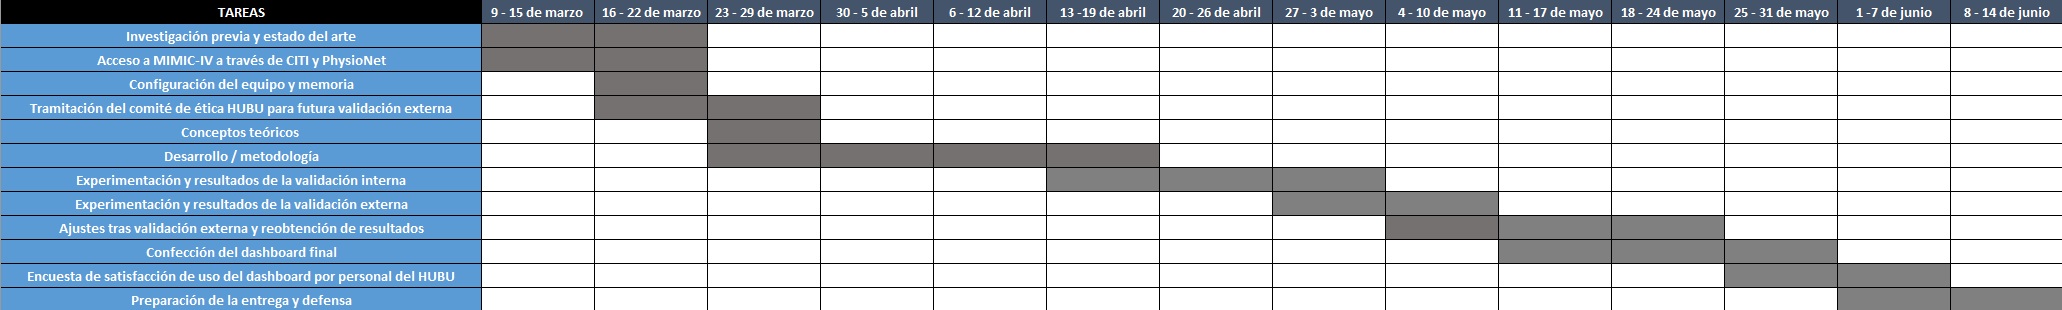
\includegraphics[width=\textwidth]{Gantt_inicial.png}
  \caption{Planificación inicial del proyecto (marzo -- junio 2026).}
  \label{fig:gantt}
\end{figure}

\begin{figure}[H]
  \centering
  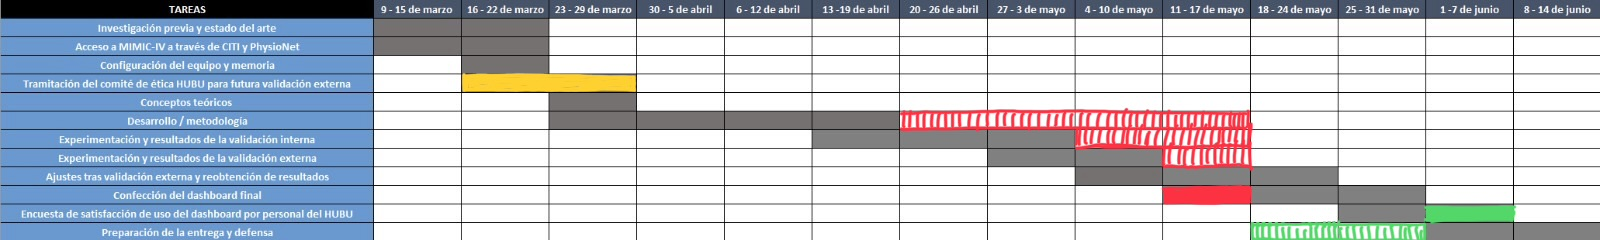
\includegraphics[width=\textwidth]{Gantt_real.jpeg}
  \caption{Ejecución real del proyecto (marzo -- junio 2026).}
  \label{fig:gantt-real}
\end{figure}

\textbf{Leyenda de colores:}
\begin{itemize}
  \item \textbf{Amarillo:} tarea no realizada, sustituida por la obtención y uso de eICU-CRD como cohorte de validación externa.
  \item \textbf{Rojo:} retraso en el inicio de la tarea respecto a la planificación inicial.
  \item \textbf{Barras rojas:} tiempo adicional necesario para completar la tarea.
  \item \textbf{Verde:} tarea finalizada antes de lo previsto.
  \item \textbf{Barras verdes:} tarea iniciada con anterioridad a lo planificado.
\end{itemize}

Las desviaciones respecto a la planificación inicial se debieron principalmente a dos causas. Los retrasos se produjeron al encontrar dificultades no anticipadas o al haber subestimado la complejidad de determinadas tareas. Los adelantos respondieron al motivo contrario: tareas cuya dificultad o duración resultó inferior a la estimada inicialmente.

El seguimiento del proyecto se organizó en GitHub mediante \textit{milestones} e \textit{issues}, agrupando las tareas en siete fases: (1)~obtención de datos y formación CITI/PhysioNet, (2)~trámites universitarios y revisión de viabilidad legal, (3)~investigación inicial y estado del arte, (4)~definición de la cohorte y extracción de MIMIC-IV, (5)~validación externa sobre eICU-CRD, (6)~desarrollo del \textit{dashboard} y (7)~redacción de la memoria y los anexos.

Las fases vinculadas a la obtención de datos, construcción de cohortes, experimentación principal y validación externa se completaron dentro del alcance finalmente definido. El desarrollo del \textit{dashboard} y la redacción de la memoria constituyeron la etapa final del trabajo, concentrada en las últimas semanas de mayo y primera de junio. La experimentación interna —entrenamiento, calibración e iteración sucesiva de los modelos— se gestionó por versiones en el repositorio en lugar de como un \textit{milestone} independiente, tal como refleja la sucesión de carpetas de pruebas descrita en el apartado anterior.

\subsection{Planificación económica}

A continuación se estima el coste que supondría ejecutar este proyecto en un contexto profesional. Se valora, por un lado, el coste material imputable, incluyendo hardware, software y datos, y por otro, el coste de personal, calculando la dedicación al precio de mercado fijado por convenio. El software empleado es de código abierto o de libre acceso y las bases de datos utilizadas no tienen coste económico directo para fines de investigación, por lo que el coste material se reduce a la amortización del equipo.

\subsubsection*{Costes materiales}

Para el desarrollo se utilizó un equipo HP Pavilion Plus con procesador Intel Core Ultra 7, 32\,GB de RAM, SSD de 1\,TB y tarjeta gráfica Nvidia RTX 4050 con 6\,GB de VRAM, adquirido en febrero de 2026 por 1.500\,€.

Suponiendo una vida útil de cinco años y una jornada anual máxima de 1.792 horas, la vida útil total estimada del equipo es:

\[
1.792 \times 5 = 8.960\ \text{h}
\]

El coste horario de amortización es, por tanto:

\[
\frac{1.500}{8.960} \approx 0{,}167\ \text{€/h}
\]

Dado que el proyecto requirió 360 horas de trabajo, el coste de hardware imputable asciende a:

\[
\frac{1.500}{8.960} \times 360 = 60{,}27\ \text{€}
\]

\begin{table}[H]
\centering
\caption{Estimación de costes materiales del proyecto.}
\label{tab:costes_materiales}
\begin{tabular}{llr}
\toprule
\textbf{Categoría} & \textbf{Concepto} & \textbf{Coste} \\
\midrule
Hardware  & Amortización proporcional del portátil & 60,27\,€ \\
Software  & Python, SQL y R en VS Code y PostgreSQL & 0,00\,€ \\
Datos     & MIMIC-IV y eICU-CRD (PhysioNet) & 0,00\,€ \\
\midrule
\multicolumn{2}{r}{\textbf{Total costes materiales}} & \textbf{60,27\,€} \\
\bottomrule
\end{tabular}
\end{table}

\subsubsection*{Costes de personal}

Para estimar el coste de personal se toma como referencia el XX Convenio colectivo nacional de empresas de ingeniería, oficinas de estudios técnicos, inspección, supervisión y control técnico y de calidad. Según la clasificación profesional recogida en dicho convenio, un graduado universitario se encuadra en el Nivel Salarial 2. La actualización de las tablas salariales para 2024 fija para este nivel una retribución total anual de 22.224,26\,€ brutos, incluyendo la tabla salarial anual y el plus de convenio.

Considerando la jornada anual máxima de 1.792 horas establecida en el convenio, el coste salarial horario equivalente es:

\[
\frac{22.224{,}26}{1.792} \approx 12{,}40\ \text{€/h}
\]

Para las 360 horas de dedicación, el salario bruto proporcional asciende a:

\[
\frac{22.224{,}26}{1.792} \times 360 = 4.464{,}70\ \text{€}
\]

A este importe se añaden las cotizaciones empresariales a la Seguridad Social. A efectos de estimación, se aplica un porcentaje conjunto del 32,30\,\% sobre el salario bruto, formado por las aportaciones empresariales por contingencias comunes, desempleo, FOGASA, formación profesional, Mecanismo de Equidad Intergeneracional y una estimación de contingencias profesionales. Estas últimas dependen de la tarifa de primas aplicable, por lo que el porcentaje empleado debe interpretarse como una aproximación razonable para la estimación económica del proyecto.

\[
4.464{,}70 \times 0{,}3230 = 1.442{,}10\ \text{€}
\]

Por tanto, el coste de personal estimado es:

\[
4.464{,}70 + 1.442{,}10 = 5.906{,}80\ \text{€}
\]

\begin{table}[H]
\centering
\caption{Estimación del coste de personal del proyecto.}
\label{tab:coste_laboral}
\begin{tabular}{lrr}
\toprule
\textbf{Concepto} & \textbf{Cálculo} & \textbf{Importe} \\
\midrule
Salario bruto proporcional & 12,40\,€/h $\times$ 360\,h & 4.464,70\,€ \\
Cotizaciones empresariales estimadas & 32,30\,\% $\times$ 4.464,70\,€ & 1.442,10\,€ \\
\midrule
\textbf{Coste de personal} &  & \textbf{5.906,80\,€} \\
\bottomrule
\end{tabular}
\end{table}

\subsubsection*{Costes indirectos y coste total}

No se imputan costes indirectos (electricidad, conexión a internet o espacio de trabajo) de forma separada, al haberse desarrollado el proyecto con recursos personales y sin instalaciones dedicadas; su efecto se considera marginal frente a los costes de personal y se omite de forma deliberada.

Sumando los costes materiales y de personal, el coste total estimado de ejecución del proyecto es:

\[
60{,}27 + 5.906{,}80 = 5.967{,}07\ \text{€}
\]

\begin{table}[H]
\centering
\caption{Coste total estimado del proyecto.}
\label{tab:coste_total}
\begin{tabular}{lr}
\toprule
\textbf{Concepto} & \textbf{Importe} \\
\midrule
Costes materiales & 60,27\,€ \\
Coste de personal & 5.906,80\,€ \\
\midrule
\textbf{Coste total estimado} & \textbf{5.967,07\,€} \\
\bottomrule
\end{tabular}
\end{table}

Este importe no representa un precio de venta o de facturación, sino una estimación del coste interno de ejecución, considerando la amortización del equipo, el salario bruto proporcional y las cotizaciones empresariales estimadas a la Seguridad Social. Todas las operaciones se han calculado sobre los valores exactos, no sobre los redondeos intermedios mostrados en las fórmulas.

\subsection{Viabilidad legal}

Dado que este trabajo constituye un análisis retrospectivo sobre bases de datos públicas y desidentificadas por sus custodios originales \citep{johnson2023,pollard2018,physionet}, el análisis desarrollado en este TFG no requirió una aprobación adicional por parte de un Comité de Ética de Investigación local. El acceso a MIMIC-IV y eICU-CRD a través de PhysioNet exige acreditar formación en ética de la investigación con datos de sujetos humanos y suscribir el correspondiente acuerdo de uso de datos. Por ello, se aporta la certificación del CITI Program completada por el autor como documento acreditativo de dicha formación.

La formación corresponde al curso \emph{Human Research — Data or Specimens Only Research (Stage 1, Basic Course)}, completado el 14 de marzo de 2026 con una puntuación de 95 sobre un mínimo exigido de 90 (Record ID 75910225), e incluyó módulos sobre el Informe Belmont, regulación y revisión por IRB, investigación basada en registros (\emph{Records-Based Research}), protecciones de privacidad HIPAA y conflictos de interés, entre otros. El certificado se muestra en la Figura~\ref{fig:citi-cert} y el informe detallado de módulos en la Figura~\ref{fig:citi-report}.

No obstante, para continuar con una validación externa con datos del Hospital Universitario de Burgos o para validar el \textit{dashboard} como herramienta clínica, sí se precisaría la aprobación del Comité de Ética de Investigación correspondiente. Por este motivo, en este anexo se incluye la acreditación disponible para el alcance finalmente desarrollado, y se explicita que cualquier extensión del trabajo a datos locales o a validación prospectiva requeriría autorización ética específica.

\begin{figure}[H]
  \centering
  
\includegraphics[width=0.85\textwidth]{citi_certificado.png}
  \caption{Certificado de finalización del curso CITI Program.}
  \label{fig:citi-cert}
\end{figure}

\begin{figure}[H]
  \centering
  
\includegraphics[width=0.85\textwidth]{citi_informe.png}
  \caption{Informe de finalización del CITI Program con el detalle de módulos y puntuaciones, se censura información de carácter personal.}
  \label{fig:citi-report}
\end{figure}

%% ══════════════════════════════════════════════════════
%%  APÉNDICE B – Especificación de Diseño
%% ══════════════════════════════════════════════════════
\apendice{Manual de especificación de diseño}

\section{Diseño arquitectónico}

El sistema desarrollado se organiza en dos subsistemas principales y desacoplados: un \textit{pipeline} de modelado y entrenamiento, encargado de transformar los datos clínicos en modelos 
predictivos entrenados, calibrados e interpretables; y una aplicación de visualización o \textit{dashboard}, encargada de cargar dichos modelos y aplicarlos sobre los datos introducidos 
para un paciente concreto. La Figura~\ref{fig:arquitectura} resume la arquitectura general del sistema.

El \textit{pipeline} de modelado constituye la parte experimental del proyecto. Su flujo comienza con las fuentes de datos, principalmente MIMIC-IV para el entrenamiento y eICU-CRD para la 
validación externa. A partir de estas bases se realiza la extracción de cohortes mediante consultas SQL, seguida del preprocesamiento de los datos, la selección de variables, el entrenamiento 
de los modelos, la optimización mediante validación cruzada anidada y la calibración probabilística. Finalmente, los modelos seleccionados se serializan en formato \texttt{.pkl} mediante 
\texttt{joblib}, separando así la fase de entrenamiento de la fase posterior de inferencia.

La aplicación de visualización, implementada en Streamlit, funciona como un módulo independiente que consume los modelos ya entrenados. El usuario carga un fichero CSV con mediciones
 clínicas del paciente, estructurado como registros temporales. A partir de estos datos, la aplicación calcula los estadísticos agregados requeridos por el modelo según la ventana temporal
  seleccionada, carga el modelo correspondiente, obtiene la probabilidad estimada de inicio de noradrenalina y contextualiza el resultado mediante un percentil de riesgo respecto a la cohorte
   de referencia. Este prototipo incorpora controles básicos de error durante la carga y el procesamiento del fichero, principalmente ante columnas ausentes o fallos de lectura.

Además de la probabilidad estimada, el \textit{dashboard} incorpora una explicación individual mediante valores SHAP, mostrando qué variables contribuyen a aumentar o reducir la predicción
para el paciente evaluado. De este modo, la arquitectura no se limita a producir una salida numérica, sino que integra también una capa de interpretabilidad orientada a facilitar la revisión
crítica del resultado.

La separación entre entrenamiento e inferencia permite que los modelos finales puedan reutilizarse sin repetir el proceso completo de entrenamiento. Esta decisión simplifica el uso del prototipo,
 reduce el coste computacional durante la ejecución del \textit{dashboard} y mantiene una frontera clara entre el desarrollo experimental de los modelos y su uso posterior como herramienta de 
 visualización.

\begin{figure}[H]
  \centering
  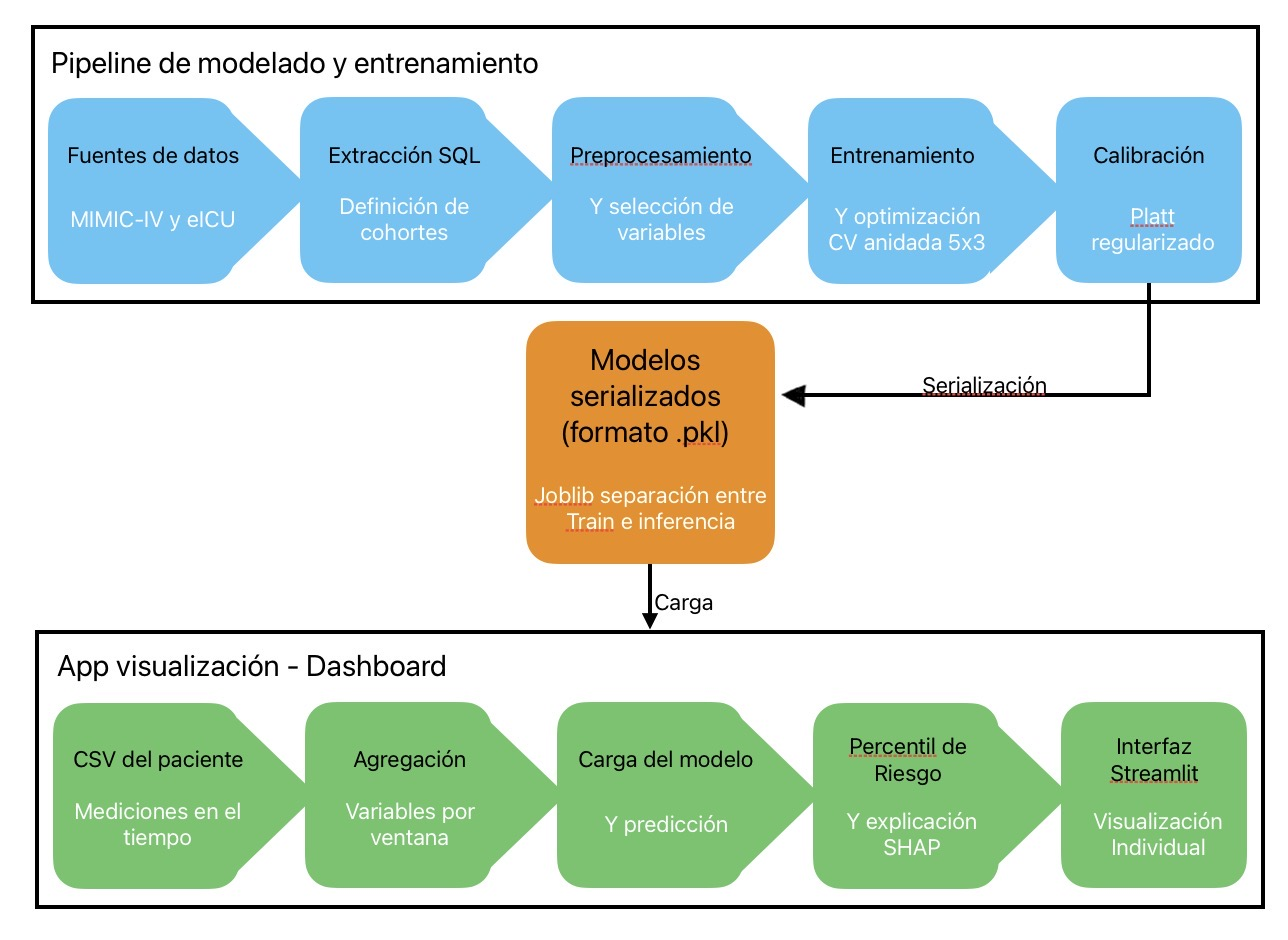
\includegraphics[width=\textwidth]{arquitectura.jpeg}
  \caption{Arquitectura general del sistema: \textit{pipeline} de modelado y entrenamiento, serialización de modelos y aplicación de visualización mediante \textit{dashboard}.}
  \label{fig:arquitectura}
\end{figure}

El diseño adoptado es deliberadamente modular. Las etapas de extracción, preprocesamiento, entrenamiento, calibración, interpretabilidad y visualización pueden modificarse de forma independiente,
 siempre que se mantenga la compatibilidad entre las variables requeridas por los modelos serializados y las variables calculadas por el \textit{dashboard}. Esta modularidad facilita la 
 trazabilidad del flujo experimental y permitiría, en trabajos futuros, sustituir modelos, actualizar cohortes o integrar nuevas fuentes de datos sin rediseñar por completo la aplicación.

%% ══════════════════════════════════════════════════════
%%  APÉNDICE C – Especificación de Requisitos
%% ══════════════════════════════════════════════════════

\apendice{Especificación de Requisitos}

\section{Diagrama de casos de uso}

El único subsistema interactivo del trabajo es el dashboard; el pipeline
de modelado se ejecuta de forma desatendida y no requiere interacción
directa por parte del usuario final. Por este motivo, los casos de uso modelan
exclusivamente la aplicación de visualización. El actor único considerado es
el facultativo de Medicina Intensiva como usuario evaluador del prototipo.
La Figura C.1 resume las funcionalidades principales.

\begin{figure}[H]
  \centering
  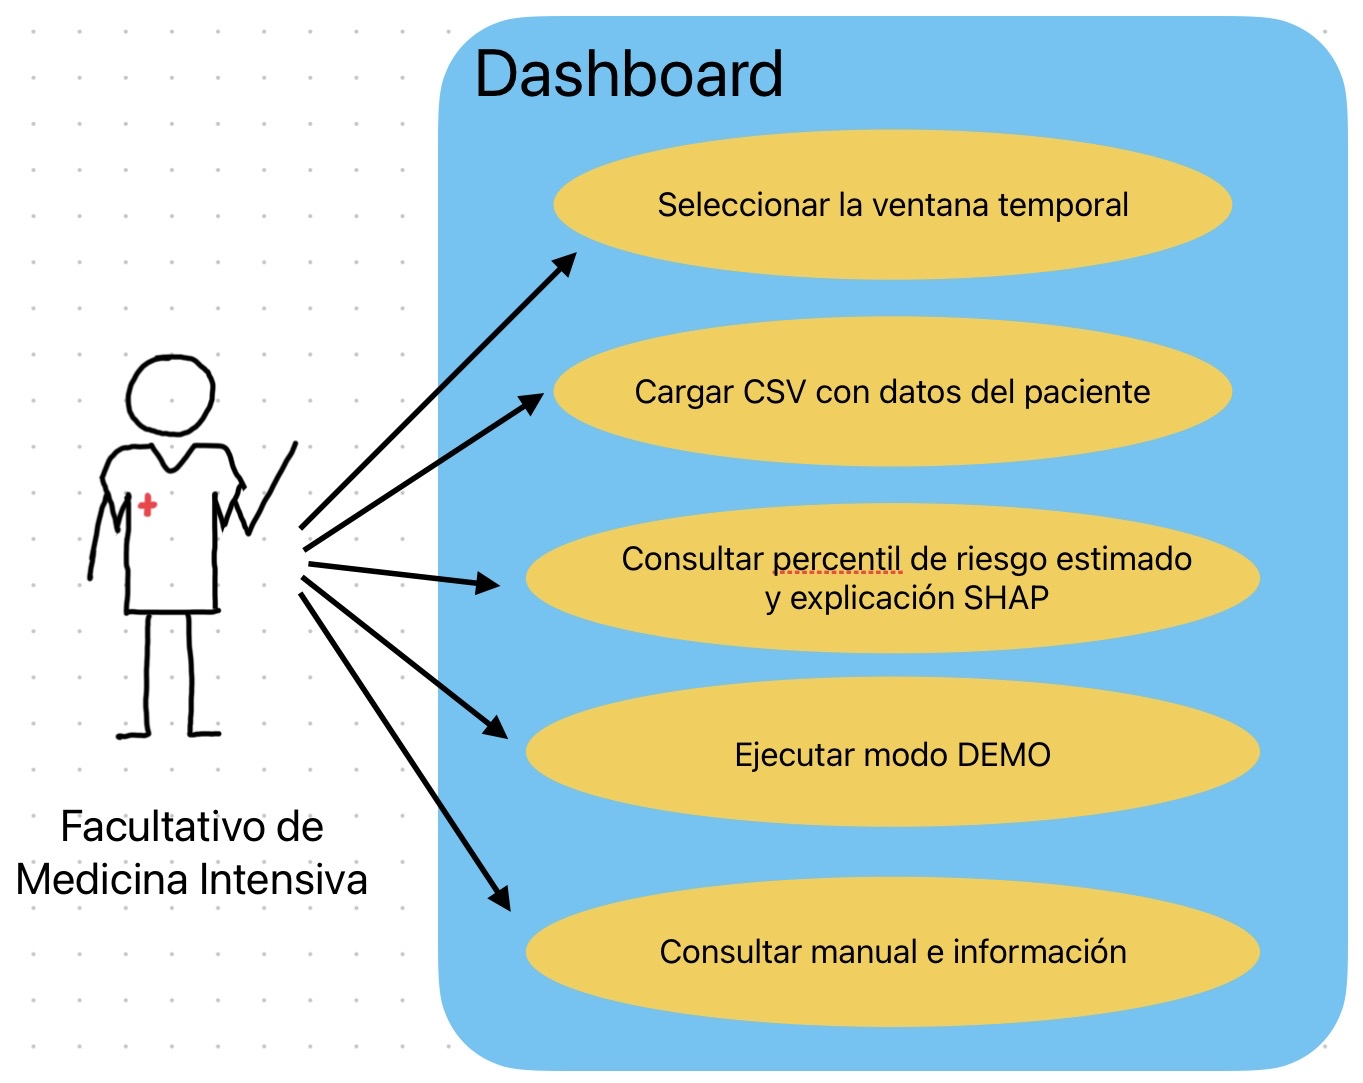
\includegraphics[width=\textwidth]{casos.jpeg}
  \caption{Diagrama de casos de uso del \textit{dashboard}.}
  \label{fig:casos-uso}
\end{figure}

\section{Explicación de los casos de uso}

A modo de contexto, los casos de uso se apoyan en los siguientes requisitos funcionales (RF) y no funcionales (RNF):

\textbf{Requisitos funcionales:}
\begin{itemize}
  \item \textbf{RF-1:} permitir seleccionar la ventana temporal de predicción disponible en el prototipo: media (6--24\,h) o larga (12--48\,h).
  \item \textbf{RF-2:} permitir cargar un fichero CSV con las mediciones clínicas del caso evaluado.
  \item \textbf{RF-3:} calcular los estadísticos agregados requeridos por el modelo a partir de las mediciones temporales del CSV.
  \item \textbf{RF-4:} cargar el modelo correspondiente a la ventana seleccionada y calcular la estimación de riesgo.
  \item \textbf{RF-5:} mostrar el riesgo estimado como percentil respecto a la distribución de referencia de MIMIC-IV.
  \item \textbf{RF-6:} mostrar la explicación individual de la predicción mediante valores SHAP.
  \item \textbf{RF-7:} disponer de un modo demostración con casos ficticios.
  \item \textbf{RF-8:} ofrecer un manual de uso y un aviso visible sobre el alcance del prototipo.
\end{itemize}

\textbf{Requisitos no funcionales:}
\begin{itemize}
  \item \textbf{RNF-1 (interpretabilidad):} las salidas deben presentarse de forma comprensible para personal clínico, combinando percentil de riesgo y explicación local mediante SHAP.
  \item \textbf{RNF-2 (no prescriptivo):} la interfaz no debe emitir recomendaciones terapéuticas automáticas, proponer dosis ni sustituir la valoración médica.
  \item \textbf{RNF-3 (usabilidad):} la interfaz debe ser sencilla y permitir una navegación básica mediante botones de ventana temporal, modo demostración y manual.
  \item \textbf{RNF-4 (privacidad y uso local):} el prototipo no persiste los datos cargados ni los envía explícitamente a servicios externos dentro del flujo implementado. En cualquier uso con datos reales, la ejecución debería realizarse en un entorno controlado y con datos adecuadamente autorizados o desidentificados.
  \item \textbf{RNF-5 (portabilidad):} la aplicación debe poder ejecutarse en un equipo con un entorno Python compatible y las dependencias del proyecto instaladas, sin requerir hardware especializado.
  \item \textbf{RNF-6 (estado del producto):} la aplicación es un prototipo académico de prueba de concepto, sin validación clínica prospectiva ni autorización regulatoria; no está destinada a uso asistencial real.
  \item \textbf{RNF-7 (tolerancia básica a errores):} la aplicación debe mostrar avisos cuando falten columnas esperadas en el CSV o se produzcan errores durante el procesamiento, sin interpretar estos controles como una validación clínica exhaustiva de la calidad del dato.
\end{itemize}

% ── CU-1 ──────────────────────────────────────────────
\begin{table}[p]
    \centering
    \begin{tabularx}{\linewidth}{ p{0.21\columnwidth} p{0.71\columnwidth} }
        \toprule
        \textbf{CU-1} & \textbf{Seleccionar la ventana temporal}\\
        \toprule
        \textbf{Versión del caso de uso} & 1.0 \\
        \textbf{Autor} & Daniel Marina de la Cal \\
        \textbf{Requisitos asociados} & RF-1, RF-4 \\
        \textbf{Descripción} & El facultativo selecciona la ventana temporal de predicción disponible en el prototipo: media (6--24\,h) o larga (12--48\,h). La selección determina el modelo que se aplicará. \\
        \textbf{Precondición} & La aplicación está en ejecución. \\
        \textbf{Acciones} &
        \begin{enumerate}
            \def\labelenumi{\arabic{enumi}.}
            \tightlist
            \item El facultativo pulsa el botón de la ventana deseada.
            \item El sistema registra la ventana seleccionada.
            \item El sistema deja preparado el modelo correspondiente para su uso posterior.
        \end{enumerate}\\
        \textbf{Postcondición} & Queda seleccionada la ventana temporal y el modelo asociado. \\
        \textbf{Excepciones} & --- \\
        \textbf{Importancia} & Alta \\
        \bottomrule
    \end{tabularx}
    \caption{CU-1 Seleccionar la ventana temporal.}
\end{table}

% ── CU-2 ──────────────────────────────────────────────
\begin{table}[p]
    \centering
    \begin{tabularx}{\linewidth}{ p{0.21\columnwidth} p{0.71\columnwidth} }
        \toprule
        \textbf{CU-2} & \textbf{Cargar CSV con datos del caso evaluado}\\
        \toprule
        \textbf{Versión del caso de uso} & 1.0 \\
        \textbf{Autor} & Daniel Marina de la Cal \\
        \textbf{Requisitos asociados} & RF-2, RF-3, RNF-7 \\
        \textbf{Descripción} & El facultativo carga un fichero CSV con mediciones clínicas temporales. El sistema intenta procesar el fichero y calcular los estadísticos agregados requeridos por el modelo. \\
        \textbf{Precondición} & Haber seleccionado una ventana temporal (CU-1) y disponer de un CSV con el formato esperado. \\
        \textbf{Acciones} &
        \begin{enumerate}
            \def\labelenumi{\arabic{enumi}.}
            \tightlist
            \item El facultativo selecciona la opción de carga de datos.
            \item Elige el fichero CSV del caso evaluado.
            \item El sistema lee el fichero.
            \item El sistema calcula los estadísticos agregados necesarios para la ventana seleccionada.
            \item El sistema habilita la consulta del riesgo y la explicación.
        \end{enumerate}\\
        \textbf{Postcondición} & Los datos quedan cargados y transformados en las variables requeridas por el modelo. \\
        \textbf{Excepciones} & Si faltan columnas esperadas o se produce un error durante el procesamiento, el sistema muestra un aviso y no presenta resultados. Estos controles son básicos y no equivalen a una validación clínica exhaustiva del CSV. \\
        \textbf{Importancia} & Alta \\
        \bottomrule
    \end{tabularx}
    \caption{CU-2 Cargar CSV con datos del caso evaluado.}
\end{table}

% ── CU-3 ──────────────────────────────────────────────
\begin{table}[p]
    \centering
    \begin{tabularx}{\linewidth}{ p{0.21\columnwidth} p{0.71\columnwidth} }
        \toprule
        \textbf{CU-3} & \textbf{Consultar el percentil de riesgo y la explicación SHAP}\\
        \toprule
        \textbf{Versión del caso de uso} & 1.0 \\
        \textbf{Autor} & Daniel Marina de la Cal \\
        \textbf{Requisitos asociados} & RF-4, RF-5, RF-6, RNF-1, RNF-2 \\
        \textbf{Descripción} & El facultativo consulta el riesgo estimado de inicio de noradrenalina, expresado como percentil respecto a la población de referencia, junto con la explicación individual de las variables que contribuyen a la predicción. \\
        \textbf{Precondición} & Datos del caso cargados y procesados (CU-2). \\
        \textbf{Acciones} &
        \begin{enumerate}
            \def\labelenumi{\arabic{enumi}.}
            \tightlist
            \item El sistema aplica el modelo de la ventana seleccionada.
            \item Calcula la probabilidad estimada de inicio de noradrenalina.
            \item Traduce la probabilidad a un percentil respecto a la distribución de referencia de MIMIC-IV.
            \item Muestra el percentil de riesgo.
            \item Calcula los valores SHAP individuales y muestra las variables que empujan o reducen el riesgo.
        \end{enumerate}\\
        \textbf{Postcondición} & Se muestran el percentil de riesgo y la explicación individualizada de la predicción. \\
        \textbf{Excepciones} & Si el modelo o el fichero de referencia de percentiles no está disponible, el sistema muestra un error y no calcula el resultado. \\
        \textbf{Importancia} & Alta \\
        \bottomrule
    \end{tabularx}
    \caption{CU-3 Consultar el percentil de riesgo y la explicación SHAP.}
\end{table}

% ── CU-4 ──────────────────────────────────────────────
\begin{table}[p]
    \centering
    \begin{tabularx}{\linewidth}{ p{0.21\columnwidth} p{0.71\columnwidth} }
        \toprule
        \textbf{CU-4} & \textbf{Ejecutar el modo demostración}\\
        \toprule
        \textbf{Versión del caso de uso} & 1.0 \\
        \textbf{Autor} & Daniel Marina de la Cal \\
        \textbf{Requisitos asociados} & RF-7 \\
        \textbf{Descripción} & El facultativo explora el funcionamiento del \textit{dashboard} con casos ficticios, sin necesidad de cargar un CSV propio. \\
        \textbf{Precondición} & La aplicación está en ejecución. \\
        \textbf{Acciones} &
        \begin{enumerate}
            \def\labelenumi{\arabic{enumi}.}
            \tightlist
            \item El facultativo pulsa el botón de modo demostración.
            \item Selecciona uno de los casos ficticios disponibles.
            \item Selecciona la ventana temporal de demostración.
            \item El sistema muestra los datos del caso, el percentil de riesgo y la explicación SHAP correspondientes.
        \end{enumerate}\\
        \textbf{Postcondición} & Se muestra el resultado del caso de demostración seleccionado. \\
        \textbf{Excepciones} & Si no se puede cargar el modelo o la referencia de percentiles, el sistema muestra un error. \\
        \textbf{Importancia} & Baja \\
        \bottomrule
    \end{tabularx}
    \caption{CU-4 Ejecutar el modo demostración.}
\end{table}

% ── CU-5 ──────────────────────────────────────────────
\begin{table}[p]
    \centering
    \begin{tabularx}{\linewidth}{ p{0.21\columnwidth} p{0.71\columnwidth} }
        \toprule
        \textbf{CU-5} & \textbf{Consultar el manual e información}\\
        \toprule
        \textbf{Versión del caso de uso} & 1.0 \\
        \textbf{Autor} & Daniel Marina de la Cal \\
        \textbf{Requisitos asociados} & RF-8, RNF-2, RNF-6 \\
        \textbf{Descripción} & El facultativo consulta el manual de uso integrado, que documenta las ventanas disponibles, el formato esperado del CSV, la interpretación de los resultados y el aviso de prototipo. \\
        \textbf{Precondición} & La aplicación está en ejecución. \\
        \textbf{Acciones} &
        \begin{enumerate}
            \def\labelenumi{\arabic{enumi}.}
            \tightlist
            \item El facultativo pulsa el botón de manual / información.
            \item El sistema muestra las instrucciones de uso.
            \item El sistema muestra el aviso de alcance del prototipo.
        \end{enumerate}\\
        \textbf{Postcondición} & Se muestra la documentación de uso en pantalla. \\
        \textbf{Excepciones} & --- \\
        \textbf{Importancia} & Baja-media \\
        \bottomrule
    \end{tabularx}
    \caption{CU-5 Consultar el manual e información.}
\end{table}

\section{Prototipo de interfaz}

\begin{figure}[H]
  \centering
  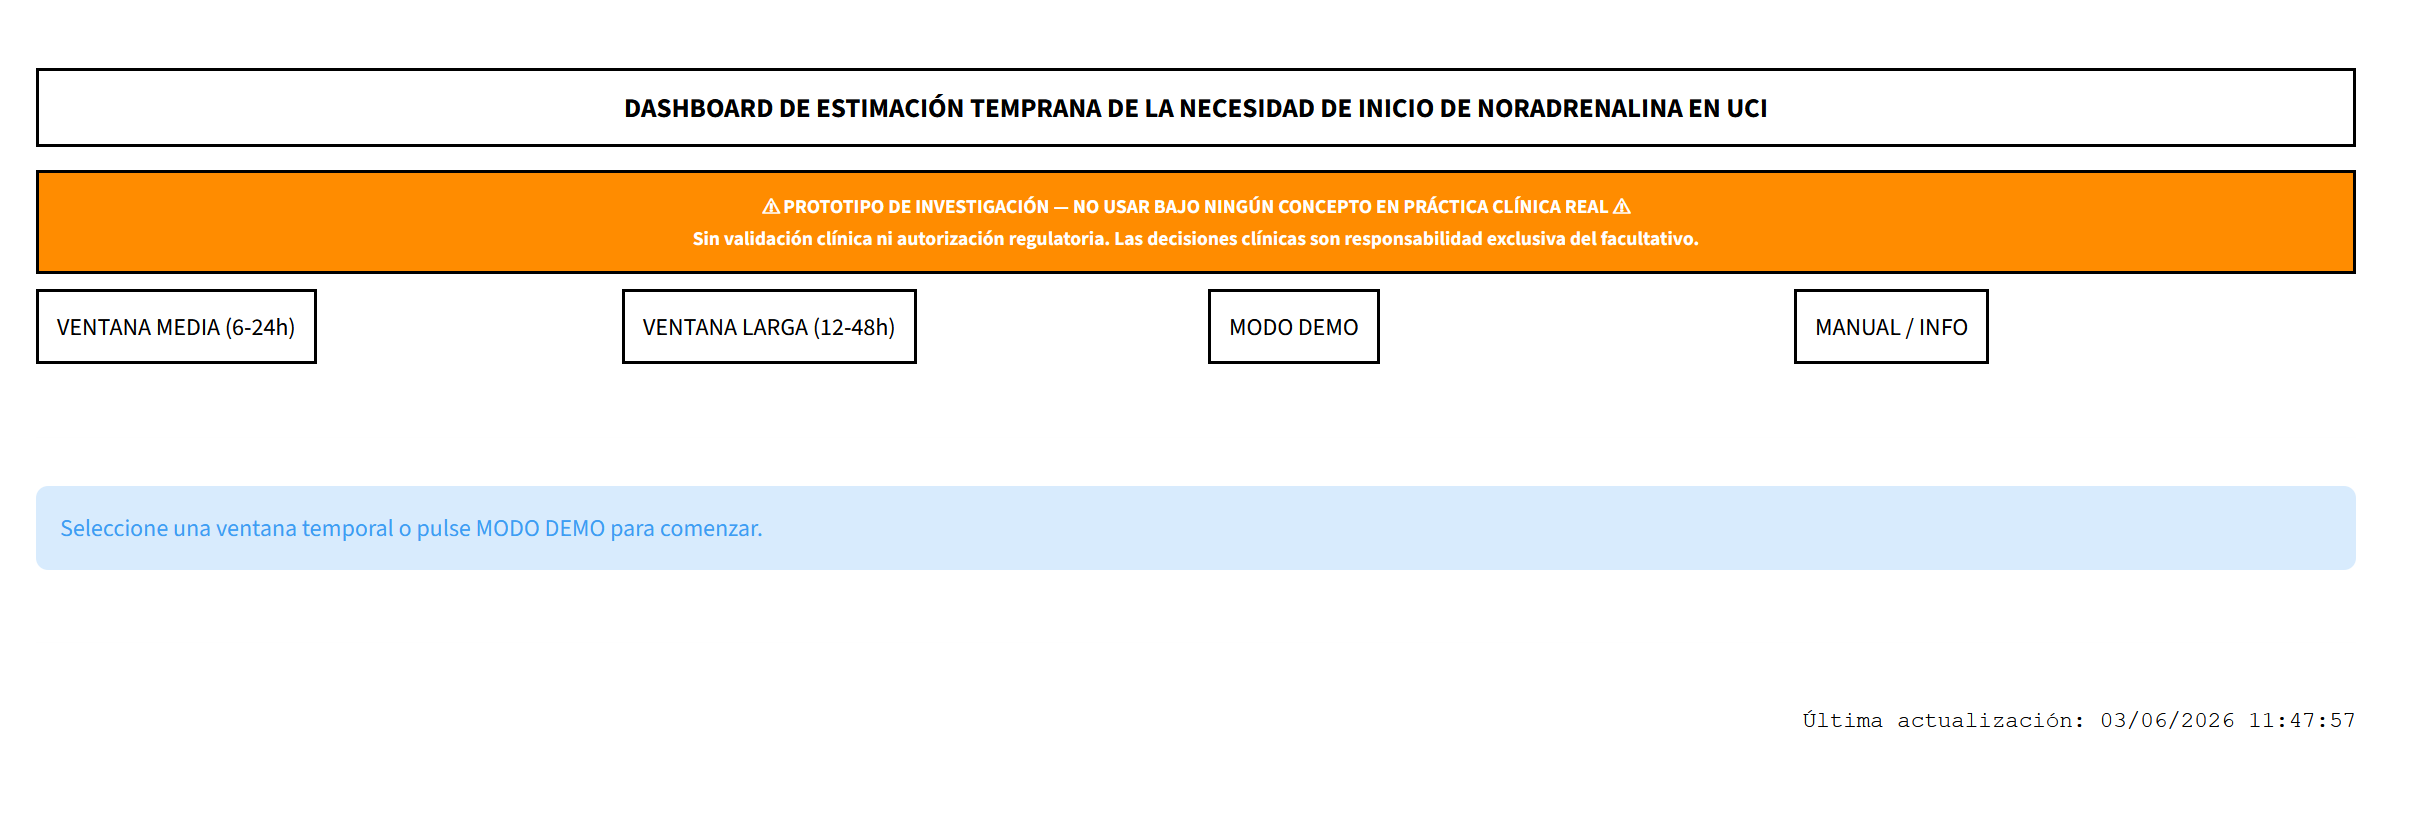
\includegraphics[width=\textwidth]{dashboard_portada.png}
  \caption{Pantalla de inicio del \textit{dashboard}. Bajo el título se muestra el aviso permanente de prototipo de investigación y los controles de selección de ventana temporal, modo demostración y manual. La aplicación no realiza ninguna estimación hasta que el usuario selecciona una opción.}
  \label{fig:dash-portada}
\end{figure}

\begin{figure}[H]
  \centering
  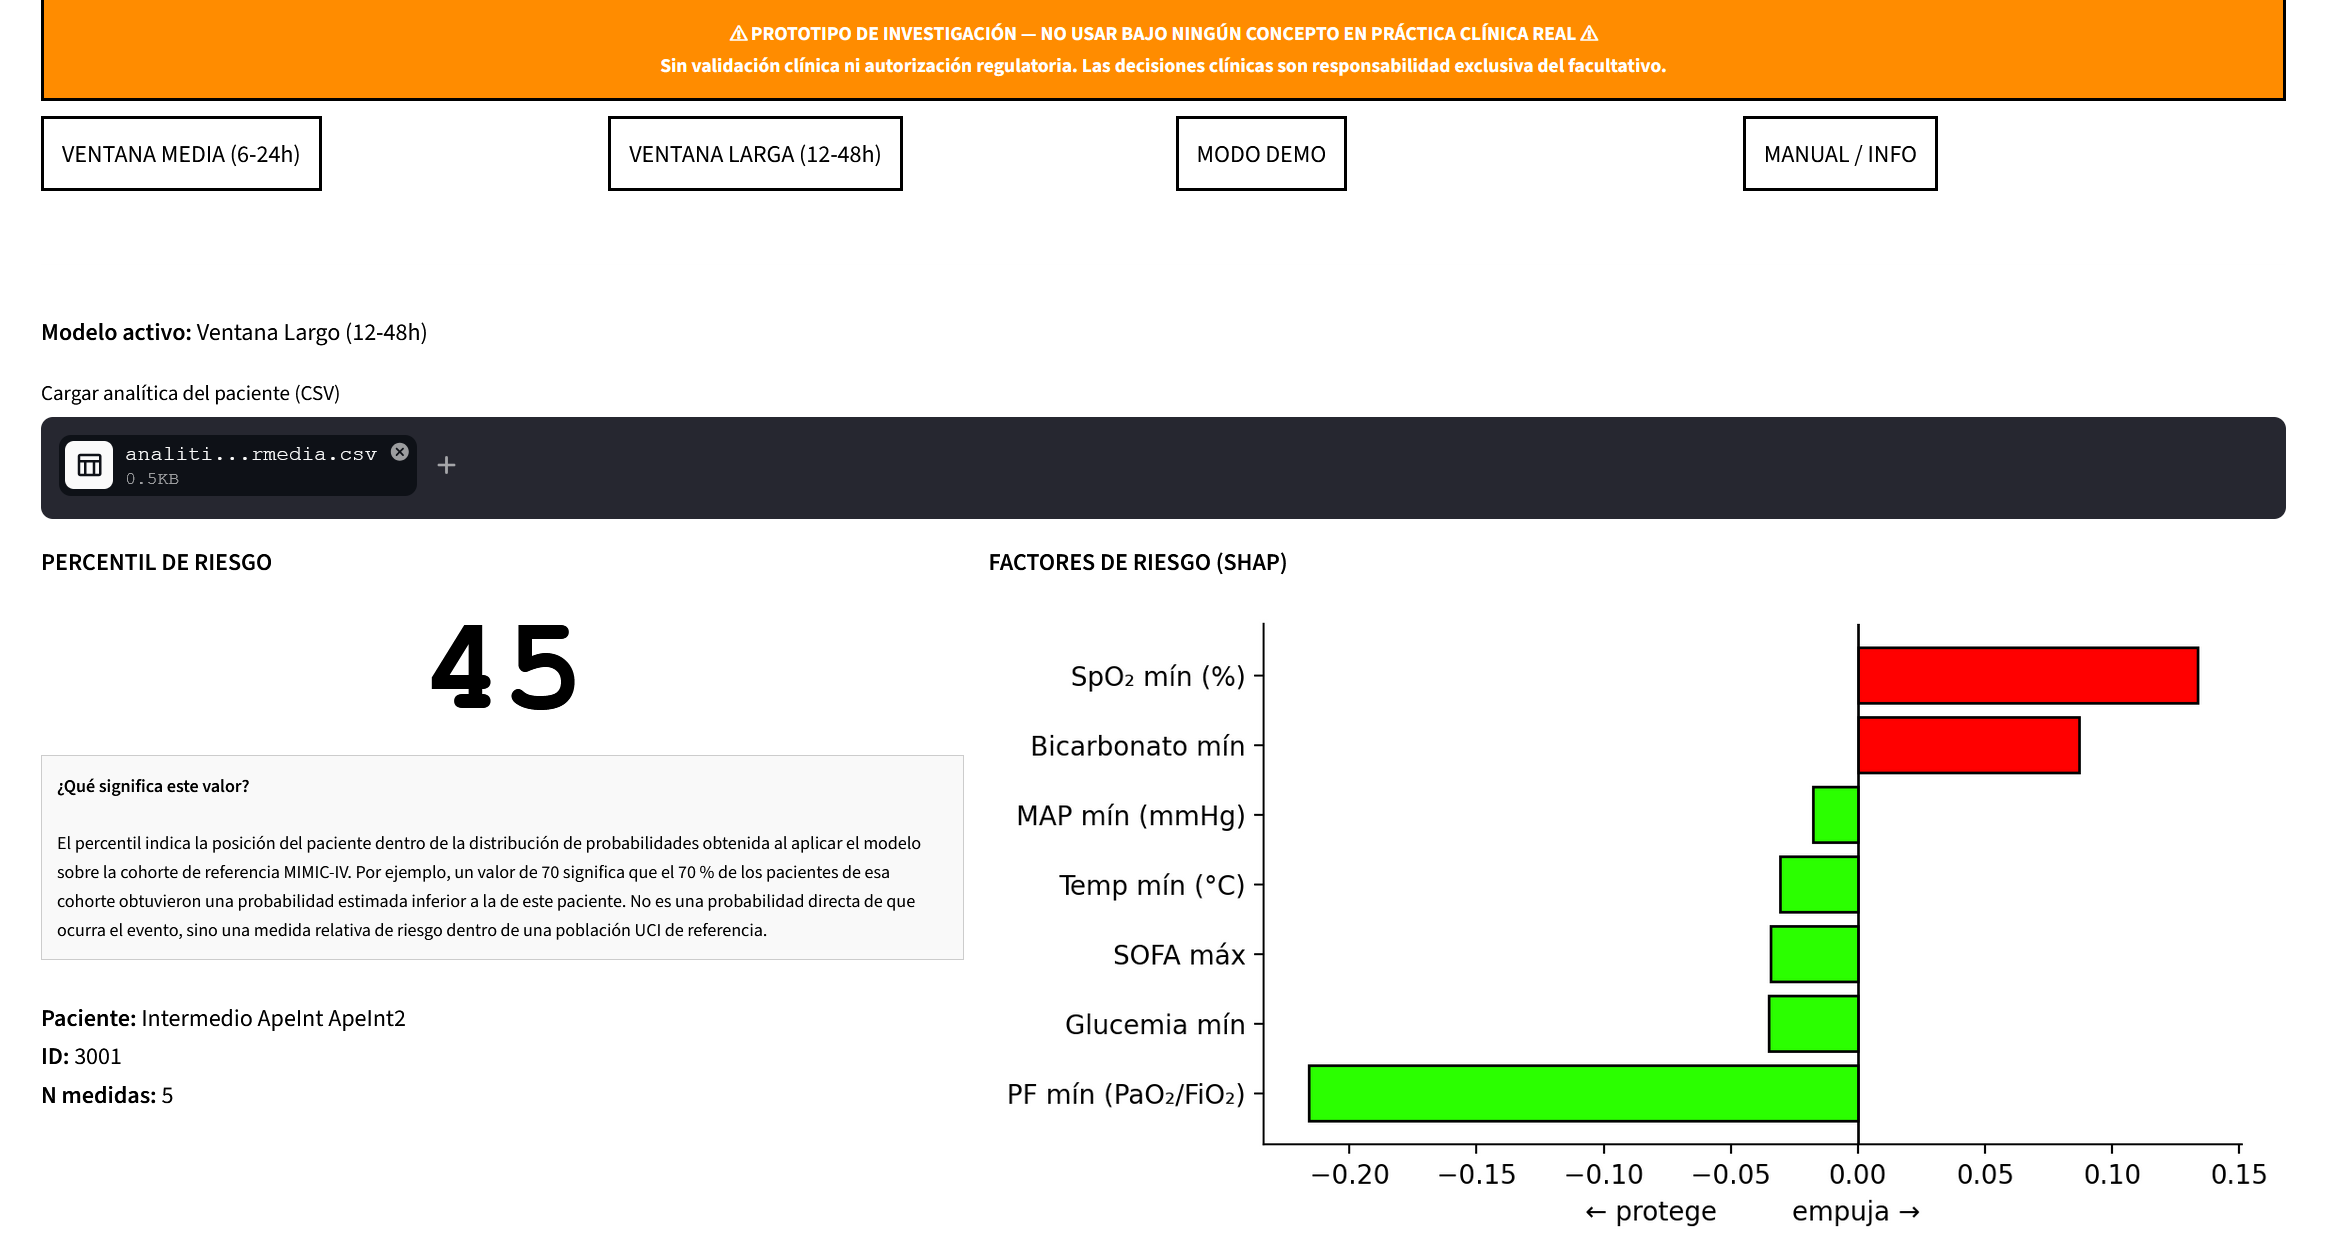
\includegraphics[width=\textwidth]{dashboard.png}
  \caption{Vista principal tras cargar los datos de un caso ficticio en la ventana larga (12--48\,h). A la izquierda se muestra el percentil de riesgo acompañado de su explicación textual y de los datos del caso; a la derecha, los factores individuales según los valores SHAP, donde las barras rojas empujan el riesgo al alza y las verdes lo reducen.}
  \label{fig:dash-principal}
\end{figure}

\begin{figure}[H]
  \centering
  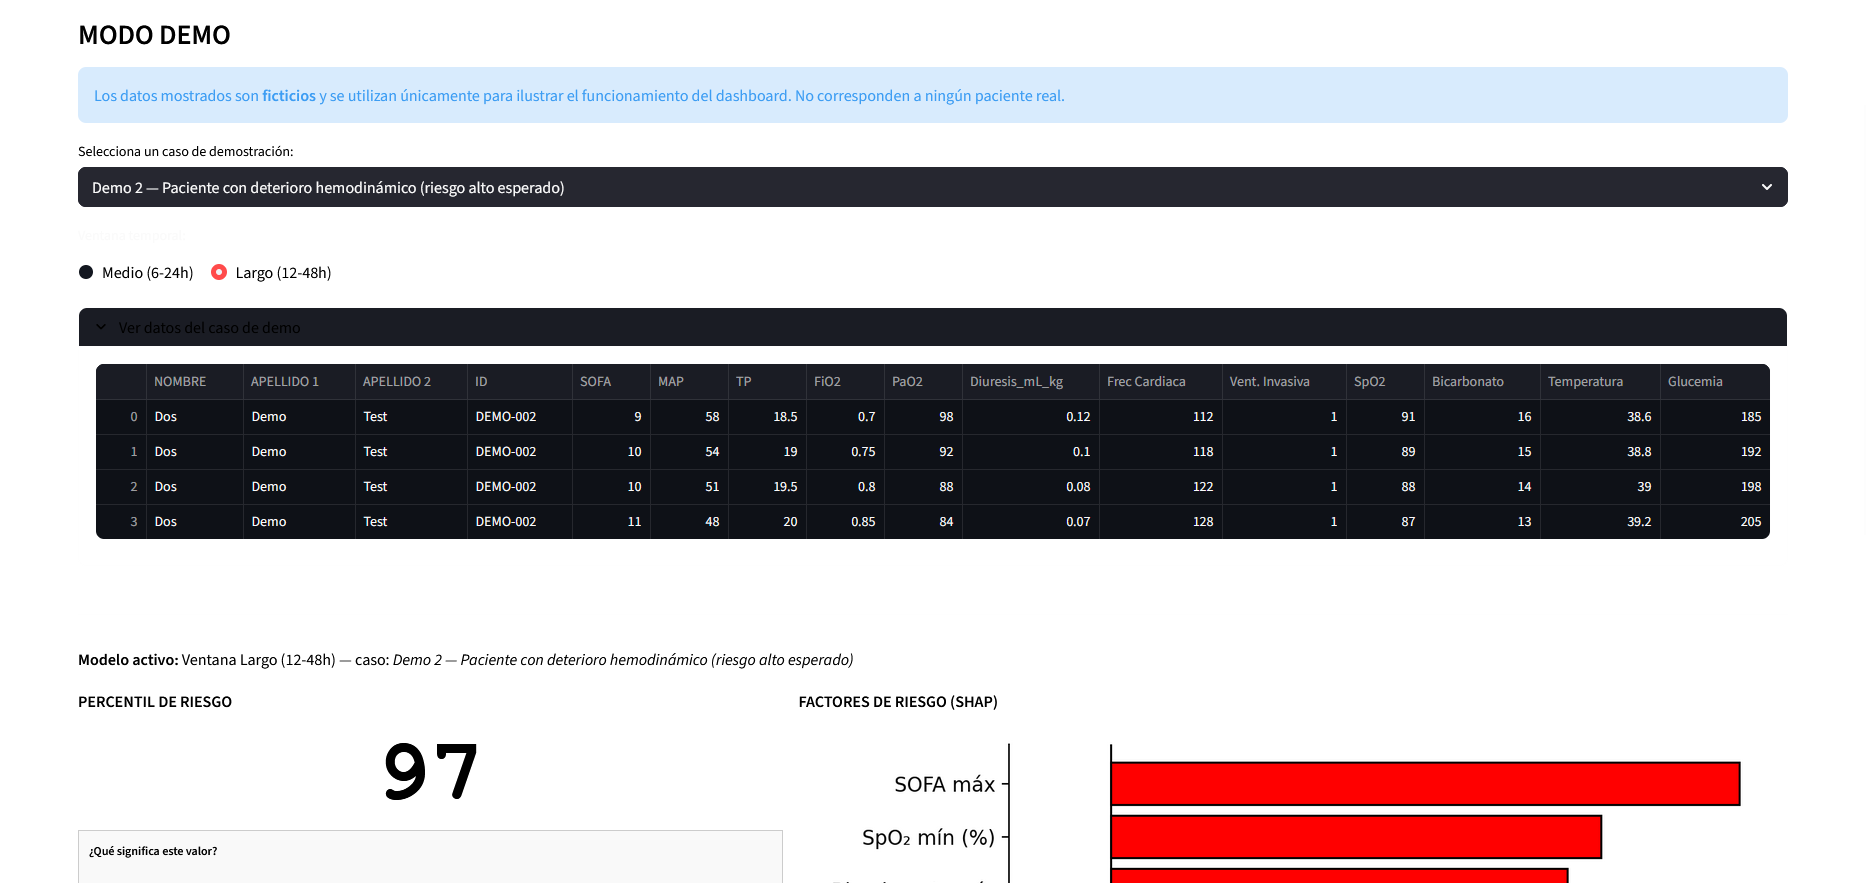
\includegraphics[width=\textwidth]{dashboard_demo.png}
  \caption{Modo demostración. Permite explorar el funcionamiento del \textit{dashboard} con casos ficticios, sin necesidad de cargar un CSV propio. Se muestra un caso de paciente con deterioro hemodinámico.}
  \label{fig:dash-demo}
\end{figure}

\begin{figure}[H]
  \centering
  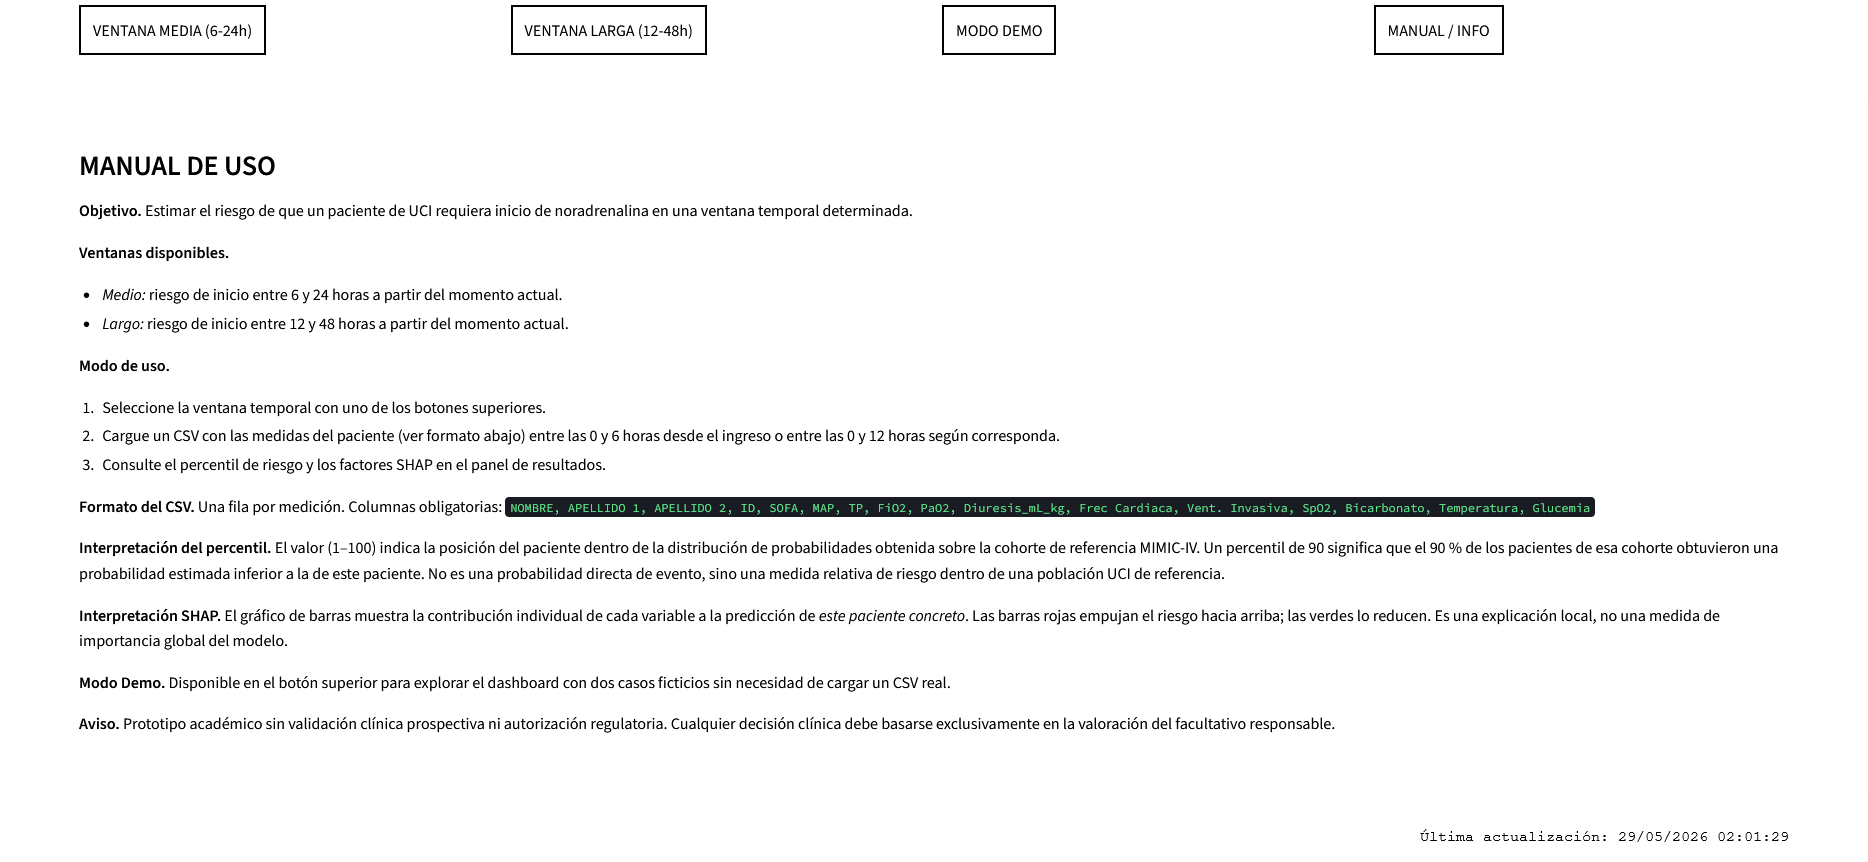
\includegraphics[width=\textwidth]{dashboard_manual.png}
  \caption{Manual de uso integrado, accesible desde la propia interfaz. Documenta las ventanas temporales disponibles, el modo de uso, el formato esperado del CSV de entrada y la interpretación del percentil de riesgo y de los valores SHAP.}
  \label{fig:dash-manual}
\end{figure}

%% ══════════════════════════════════════════════════════
%%  APÉNDICE D – Manual de Usuario
%% ══════════════════════════════════════════════════════
\apendice{Documentación de usuario}

\section{Requisitos previos}

Este manual está dirigido al uso del prototipo de \textit{dashboard} por parte de personal clínico o técnico del hospital. La aplicación permite introducir datos clínicos de un paciente o caso 
de ejemplo y visualizar una estimación relativa del riesgo de inicio de noradrenalina, junto con una explicación individual mediante valores SHAP.

El usuario final previsto es un facultativo o profesional sanitario que consulta la interfaz ya en ejecución. La instalación inicial, en cambio, debería ser realizada por personal 
técnico o por una persona con conocimientos básicos de Python, ya que requiere preparar un entorno local y ejecutar una aplicación Streamlit.

La ejecución del \textit{dashboard} no requiere descargar ni acceder directamente a las bases de datos MIMIC-IV o eICU-CRD. Los modelos ya han sido entrenados previamente y se distribuyen como 
ficheros serializados en formato \texttt{.pkl}. Por tanto, el uso descrito en este manual corresponde exclusivamente a la fase de inferencia y visualización, no al reentrenamiento completo 
del sistema.

\subsection*{Requisitos de hardware}

Para ejecutar el prototipo se recomienda disponer de:

\begin{itemize}
  \item un ordenador personal o equipo hospitalario con sistema operativo Windows, Linux o macOS;
  \item al menos 4\,GB de memoria RAM;
  \item aproximadamente 1\,GB de espacio libre para el entorno de Python, dependencias y archivos del \textit{dashboard};
  \item no se requiere tarjeta gráfica dedicada, ya que la inferencia se ejecuta en CPU.
\end{itemize}

\subsection*{Requisitos de software}

El equipo debe disponer de:

\begin{itemize}
  \item Python 3.12 o una versión compatible;
  \item un navegador web actualizado;
  \item acceso local a la carpeta \texttt{Dashboard} del repositorio;
  \item las bibliotecas necesarias para ejecutar la aplicación: \texttt{streamlit}, \texttt{pandas}, \texttt{numpy}, \texttt{scikit-learn}, \texttt{xgboost}, \texttt{shap}, \texttt{matplotlib} y \texttt{joblib}.
\end{itemize}

La carpeta \texttt{Dashboard} debe contener los siguientes archivos:

\begin{itemize}
  \item \texttt{pruebas\_dashboard.py};
  \item \texttt{modelo\_Medio\_6\_24\_XGB\_calibrado.pkl};
  \item \texttt{modelo\_Largo\_12\_48\_XGB.pkl};
  \item \texttt{referencia\_percentiles\_medio.npy};
  \item \texttt{referencia\_percentiles\_largo.npy}.
\end{itemize}

Si alguno de estos archivos falta o se mueve a otra ubicación, la aplicación puede no cargar correctamente los modelos o las referencias utilizadas para calcular los percentiles de riesgo.

\section{Instalación y puesta en marcha}

La instalación debe realizarse una única vez en el equipo donde vaya a ejecutarse la aplicación. En un contexto hospitalario real, este paso correspondería al personal técnico. El facultativo no tendría que ejecutar comandos, sino acceder a la interfaz ya abierta en el navegador.

\subsection*{Instalación en un equipo local}

Los pasos recomendados son los siguientes:

\begin{enumerate}
  \item Descargar o clonar el repositorio del proyecto desde GitHub.

\begin{verbatim}
git clone [URL del repositorio]
\end{verbatim}

  \item Entrar en la carpeta del repositorio.

\begin{verbatim}
cd Estimacion-temprana-*
\end{verbatim}

  \item Crear un entorno virtual de Python (opcional).

\begin{verbatim}
python -m venv .venv
\end{verbatim}

  \item Activar el entorno virtual. En Windows:

\begin{verbatim}
.venv\Scripts\activate
\end{verbatim}

  En Linux o macOS:

\begin{verbatim}
source .venv/bin/activate
\end{verbatim}

  \item Instalar las dependencias principales de la aplicación.

\begin{verbatim}
pip install streamlit pandas numpy
pip install scikit-learn xgboost shap
pip install matplotlib joblib
\end{verbatim}

  \item Entrar en la carpeta del \textit{dashboard}.

\begin{verbatim}
cd Dashboard
\end{verbatim}

  \item Ejecutar la aplicación.

\begin{verbatim}
streamlit run pruebas_dashboard.py
\end{verbatim}

  \item Abrir en el navegador la dirección indicada por Streamlit. Habitualmente será:

\begin{verbatim}
http://localhost:8501
\end{verbatim}
\end{enumerate}

Una vez abierta la aplicación, el usuario clínico puede utilizarla desde el navegador sin interactuar con la terminal.

\subsection*{Comprobación inicial}

Antes de entregar la aplicación al usuario final, se recomienda que el personal técnico compruebe que:

\begin{itemize}
  \item la pantalla principal se abre correctamente;
  \item aparecen los botones de selección de ventana temporal;
  \item el botón \emph{Modo Demo} funciona;
  \item el botón \emph{Manual / Info} muestra las instrucciones integradas;
  \item los modelos de ventana media y larga cargan sin error;
  \item los ficheros \texttt{.pkl} y \texttt{.npy} permanecen en la carpeta \texttt{Dashboard}.
\end{itemize}

\section{Manual de uso}

Al iniciar el \textit{dashboard}, el usuario visualiza una pantalla de portada con el título del proyecto, los botones principales y un aviso de alcance del prototipo. Esta pantalla se muestra 
en la Figura~\ref{fig:dash-portada} del Apéndice~C.

La aplicación ofrece tres acciones principales:

\begin{itemize}
  \item seleccionar una ventana temporal de predicción;
  \item cargar un CSV con mediciones clínicas;
  \item utilizar el modo demostración con casos ficticios.
\end{itemize}

\subsection*{Paso 1: seleccionar la ventana temporal}

El usuario debe elegir una de las dos ventanas disponibles:

\begin{itemize}
  \item \textbf{Ventana media (6--24\,h):} estima el riesgo relativo de inicio de noradrenalina en el intervalo comprendido entre las 6 y las 24 horas.
  \item \textbf{Ventana larga (12--48\,h):} estima el riesgo relativo de inicio de noradrenalina en el intervalo comprendido entre las 12 y las 48 horas.
\end{itemize}

La selección de la ventana determina qué modelo se carga internamente. El prototipo final del \textit{dashboard} no incluye la ventana corta.

\subsection*{Paso 2: preparar el CSV}

El fichero de entrada debe estar en formato CSV y contener una fila por medición temporal. El objetivo es que el usuario introduzca datos clínicos ordinarios, no las variables agregadas finales utilizadas por el modelo. La aplicación calcula después los mínimos, máximos, medias o sumas necesarios según la ventana seleccionada.

Las columnas esperadas son:

\begin{verbatim}
NOMBRE, APELLIDO 1, APELLIDO 2, ID, SOFA, MAP, TP, FiO2, PaO2,
Diuresis_mL_kg, Frec Cardiaca, Vent. Invasiva, SpO2, Bicarbonato,
Temperatura, Glucemia
\end{verbatim}

El significado práctico de las columnas principales es:

\begin{itemize}
  \item \texttt{SOFA}: puntuación SOFA registrada en la medición.
  \item \texttt{MAP}: presión arterial media.
  \item \texttt{TP}: tiempo de protrombina.
  \item \texttt{FiO2}: fracción inspirada de oxígeno, introducida en escala decimal.
  \item \texttt{PaO2}: presión arterial de oxígeno.
  \item \texttt{Diuresis\_mL\_kg}: diuresis normalizada por peso.
  \item \texttt{Frec Cardiaca}: frecuencia cardiaca.
  \item \texttt{Vent. Invasiva}: indicador binario de ventilación mecánica invasiva.
  \item \texttt{SpO2}: saturación periférica de oxígeno.
  \item \texttt{Bicarbonato}: bicarbonato sérico.
  \item \texttt{Temperatura}: temperatura corporal.
  \item \texttt{Glucemia}: glucemia.
\end{itemize}

Las columnas \texttt{NOMBRE}, \texttt{APELLIDO 1}, \texttt{APELLIDO 2} e \texttt{ID} se muestran únicamente como identificación visual del caso dentro de la interfaz. En un contexto real, deberían emplearse datos debidamente autorizados o identificadores seudonimizados, de acuerdo con las normas del centro.

\subsection*{Paso 3: cargar el CSV}

Una vez seleccionada la ventana temporal, el usuario debe pulsar el botón de carga de archivo y seleccionar el CSV correspondiente al caso evaluado.

Si el archivo se carga correctamente, la aplicación calcula automáticamente las variables agregadas necesarias para el modelo. Si faltan columnas esperadas o se produce un error durante el procesamiento, la interfaz muestra un aviso. Estos controles son básicos y no constituyen una validación clínica exhaustiva de la calidad del dato.

\subsection*{Paso 4: consultar el resultado}

Tras procesar el CSV, la pantalla principal muestra dos bloques, como se observa en la Figura~\ref{fig:dash-principal} del Apéndice~C:

\begin{itemize}
  \item a la izquierda, el percentil de riesgo y un resumen del caso evaluado;
  \item a la derecha, los factores individuales asociados a la predicción mediante valores SHAP.
\end{itemize}

El resultado no debe interpretarse como una orden clínica ni como una recomendación terapéutica. La aplicación no indica si debe iniciarse noradrenalina, no propone dosis y no sustituye la valoración del facultativo responsable.

\subsection*{Interpretación del percentil de riesgo}

El percentil indica la posición del caso evaluado dentro de la distribución de probabilidades estimadas en la cohorte de referencia MIMIC-IV.

Por ejemplo, un percentil de 90 significa que el 90\,\% de los pacientes de la cohorte de referencia obtuvieron una probabilidad estimada inferior a la del caso evaluado. No significa que el paciente tenga un 90\,\% de probabilidad directa de iniciar noradrenalina. Es una medida relativa de riesgo respecto a una población de referencia.

\subsection*{Interpretación de los valores SHAP}

El gráfico SHAP muestra cómo contribuye cada variable a la predicción individual de ese caso concreto.

\begin{itemize}
  \item Las barras rojas empujan la estimación hacia mayor riesgo.
  \item Las barras verdes reducen la estimación de riesgo.
  \item La longitud de cada barra representa la magnitud de la contribución.
\end{itemize}

Esta explicación es local: describe el resultado del caso cargado, no la importancia global de las variables en todo el modelo.

\section{Modo demostración}

El botón \emph{Modo Demo} permite explorar el funcionamiento de la aplicación con casos ficticios, sin cargar un CSV propio. Esta opción está pensada para formación, demostración y comprobación inicial del sistema.

El modo demostración permite seleccionar entre casos simulados y elegir la ventana temporal. A continuación, el \textit{dashboard} muestra la tabla de datos del caso, el percentil de riesgo y la explicación SHAP correspondiente. Un ejemplo de esta pantalla se recoge en la Figura~\ref{fig:dash-demo} del Apéndice~C.

Este modo no utiliza datos reales y no debe interpretarse como una evaluación clínica.

\section{Manual integrado}

La aplicación incluye un botón \emph{Manual / Info}, accesible desde la pantalla principal. Este apartado integrado resume:

\begin{itemize}
  \item el objetivo del \textit{dashboard};
  \item las ventanas temporales disponibles;
  \item el formato esperado del CSV;
  \item la interpretación del percentil de riesgo;
  \item la interpretación de los valores SHAP;
  \item el modo demostración;
  \item las advertencias de uso.
\end{itemize}

La pantalla del manual integrado se muestra en la Figura~\ref{fig:dash-manual} del Apéndice~C.

\section{Advertencias de uso}

El \textit{dashboard} desarrollado es un prototipo académico y experimental. No está validado prospectivamente, no dispone de autorización regulatoria y no debe emplearse para tomar decisiones clínicas reales.

La aplicación no recomienda iniciar noradrenalina, no propone dosis, no genera alarmas clínicas y no sustituye la valoración médica. Su finalidad es demostrar la viabilidad técnica de integrar un modelo predictivo interpretable en una interfaz de visualización.

Cualquier uso futuro con datos reales de pacientes requeriría validación clínica, autorización ética y revisión por parte del centro sanitario correspondiente.

%% ══════════════════════════════════════════════════════
%%  APÉNDICE E – Manual del Desarrollador
%% ══════════════════════════════════════════════════════
\apendice{Manual del programador}

\section{Estructura de directorios}

El repositorio se organiza separando la documentación académica, el prototipo de \textit{dashboard}, el flujo experimental de modelado, la validación externa y las 
pruebas históricas. La estructura general entregada es la siguiente:

\begin{verbatim}
.
+-- Archivo/
|   +-- Pruebas preliminares/
+-- Dashboard/
+-- Memoria/
|   +-- img/
|   +-- qmd/
+-- Pipeline/
|   +-- Experimentos/
|   +-- FINAL/
+-- Validacion_externa/
|   +-- eICU/
\end{verbatim}

La carpeta \ruta{Archivo/} contiene pruebas preliminares y versiones antiguas del desarrollo. Se conserva por trazabilidad histórica, pero no constituye la referencia 
principal para reproducir los resultados finales.

La carpeta \ruta{Dashboard/} contiene el prototipo de aplicación desarrollado en Streamlit. Incluye el script principal \ruta{pruebas\_dashboard.py}, los modelos finales 
serializados en formato \ruta{.pkl} y los ficheros \ruta{.npy} utilizados como referencia para calcular los percentiles de riesgo. Esta carpeta es la unidad mínima 
necesaria para ejecutar el prototipo de inferencia una vez instaladas las dependencias.

La carpeta \ruta{Memoria/} contiene la documentación académica del TFG. En \ruta{Memoria/qmd/} se almacenan los ficheros fuente en Quarto/Markdown, mientras que 
\ruta{Memoria/img/} contiene las imágenes, diagramas y capturas empleadas en la memoria y los anexos.

La carpeta \ruta{Pipeline/Experimentos/} recoge versiones intermedias del desarrollo experimental. Estas carpetas documentan la evolución metodológica del proyecto, 
incluyendo construcción de cohortes, selección de variables, reducción de predictores, análisis de significancia, comprobación de dirección del efecto y refinamiento 
progresivo de los modelos.

La carpeta \ruta{Pipeline/FINAL/} contiene la versión final del flujo experimental utilizada para generar los resultados incluidos en la memoria. En ella se almacenan los 
scripts principales, modelos entrenados, tablas de métricas, figuras de validación interna, figuras de calibración, análisis SHAP y comparaciones finales entre modelos 
o calibradores. Debe considerarse la carpeta de referencia para consultar los resultados consolidados del modelado.

La carpeta \ruta{Validacion\_externa/eICU/} contiene el material asociado a la validación externa sobre eICU-CRD: consultas SQL, scripts de adaptación, tablas, figuras y 
resultados derivados de aplicar los modelos entrenados en MIMIC-IV sobre una cohorte externa independiente.

En términos funcionales, la relación entre carpetas puede resumirse como:

\begin{itemize}
  \item \ruta{Pipeline/Experimentos/}: trazabilidad metodológica y versiones intermedias.
  \item \ruta{Pipeline/FINAL/}: entrenamiento final, calibración, modelos, métricas y SHAP.
  \item \ruta{Validacion\_externa/eICU/}: validación externa sobre eICU-CRD.
  \item \ruta{Dashboard/}: inferencia y visualización mediante Streamlit.
  \item \ruta{Memoria/}: documentación académica.
  \item \ruta{Archivo/}: pruebas históricas no necesarias para el flujo final.
\end{itemize}

\section{Compilación y ejecución}

Este proyecto no se compila en el sentido clásico de una aplicación cerrada. El código se ejecuta mediante scripts de Python y la interfaz de usuario se lanza como una 
aplicación Streamlit. Deben distinguirse dos niveles de ejecución: el uso del \textit{dashboard}, descrito anteriormente, y la reproducción del flujo experimental.

\subsection*{Reproducción del flujo experimental}

La reproducción completa del flujo experimental requiere disponer de acceso autorizado a las bases de datos originales MIMIC-IV y eICU-CRD.

A nivel general, la reproducción sigue esta secuencia:

\begin{enumerate}
  \item Ejecutar las consultas SQL de extracción de cohortes sobre MIMIC-IV y eICU-CRD.
  \item Generar los CSV definitivos por ventana temporal.
  \item Aplicar el preprocesamiento y la selección de variables.
  \item Ejecutar los scripts finales de entrenamiento y validación interna en \ruta{Pipeline/FINAL/}.
  \item Evaluar calibración y generar figuras de validación.
  \item Calcular explicaciones SHAP.
  \item Aplicar los modelos entrenados sobre eICU-CRD en \ruta{Validacion\_externa/eICU/}.
  \item Serializar los modelos finales y referencias de percentiles para su uso en \ruta{Dashboard/}.
\end{enumerate}

La carpeta \ruta{Pipeline/FINAL/} contiene los scripts y salidas finales del modelado. Las carpetas de \ruta{Pipeline/Experimentos/} permiten reconstruir las decisiones metodológicas previas, pero no sustituyen a \ruta{Pipeline/FINAL/} como salida consolidada.

\subsection*{Compilación de la documentación}

La memoria y los anexos se encuentran en la carpeta \ruta{Memoria/}. La compilación se realiza mediante Quarto, utilizando los ficheros \ruta{.qmd} y las imágenes almacenadas en \ruta{Memoria/img/}. Desde la carpeta correspondiente puede ejecutarse:

\begin{verbatim}
quarto render anexos.qmd
\end{verbatim}

o, para la memoria principal:

\begin{verbatim}
quarto render memoria.qmd
\end{verbatim}

La compilación requiere tener instalado Quarto, una distribución LaTeX compatible y las dependencias de R/Python utilizadas por los bloques ejecutables, en caso de que el documento los incluya.

\section{Pruebas del sistema}

Al tratarse de un trabajo de investigación de carácter experimental, no se desarrolló una batería completa de pruebas unitarias, pruebas de integración o integración 
continua propia de un software de producción. La validación del sistema se abordó desde dos perspectivas: validación metodológica de los modelos y comprobación funcional 
básica del prototipo de \textit{dashboard}.

Desde el punto de vista metodológico, se aplicaron las siguientes estrategias:

\begin{itemize}
  \item \textbf{Validación interna} mediante validación cruzada anidada (5$\times$3) con agrupamiento por paciente, para evitar fugas de información entre particiones.
  \item \textbf{Validación externa} sobre la cohorte independiente y multicéntrica eICU-CRD.
  \item \textbf{Análisis por subgrupos} según presencia de sepsis, para evaluar la estabilidad del rendimiento en MIMIC-IV.
  \item \textbf{Comparación frente a SOFA} como referencia clínica de gravedad.
  \item \textbf{Evaluación de calibración} mediante ECE, Brier Score y Brier Skill Score.
  \item \textbf{Auditoría de interpretabilidad} mediante valores SHAP, comprobando la coherencia clínica de las variables con mayor contribución.
  \item \textbf{Evaluación exploratoria de usabilidad} del \textit{dashboard} mediante una encuesta a ocho facultativos del servicio de Medicina Intensiva del HUBU.
\end{itemize}

Además, para el prototipo de \textit{dashboard} se realizaron comprobaciones funcionales básicas:

\begin{itemize}
  \item apertura correcta de la aplicación en Streamlit;
  \item carga de los modelos serializados en formato \ruta{.pkl};
  \item carga de los ficheros de referencia de percentiles en formato \ruta{.npy};
  \item selección de las ventanas media y larga;
  \item ejecución del modo demostración;
  \item carga de CSV con el formato esperado;
  \item cálculo de las variables agregadas requeridas por cada modelo;
  \item visualización del percentil de riesgo;
  \item generación de la explicación individual mediante SHAP;
  \item visualización del manual integrado;
  \item aparición de avisos cuando faltan columnas o se produce un error durante el procesamiento.
\end{itemize}

Estas comprobaciones no sustituyen a una validación clínica prospectiva ni a una certificación del software como producto sanitario. Su objetivo fue verificar la coherencia
técnica del prototipo dentro del alcance académico del TFG.

Los resultados cuantitativos de la validación interna, la validación externa, la calibración, la comparación frente a SOFA y la encuesta de usabilidad se recogen en los 
capítulos de Resultados y Discusión de la memoria.

\section{Instrucciones para la modificación o mejora del proyecto}

Para facilitar futuras ampliaciones, se ofrecen las siguientes recomendaciones:

\subsection*{Validación externa pendiente con datos del HUBU}

Una ampliación prioritaria del proyecto sería realizar una validación externa local con datos del Hospital Universitario de Burgos. A diferencia del reentrenamiento, esta
 validación debería aplicar los modelos ya entrenados sobre MIMIC-IV a una cohorte independiente del HUBU, sin reajustar los parámetros del modelo, con el objetivo de
  evaluar su transportabilidad al entorno clínico local.

Para llevar a cabo esta validación sería necesario:

\begin{itemize}
  \item obtener la autorización ética y administrativa correspondiente para el uso secundario de los datos clínicos locales;
  \item definir una cohorte de pacientes de UCI equivalente a la empleada en MIMIC-IV;
  \item adaptar las consultas de extracción al sistema de información hospitalario disponible;
  \item reconstruir las mismas ventanas temporales de observación y predicción;
  \item calcular la variable objetivo de inicio de noradrenalina con la misma definición temporal;
  \item armonizar las unidades, nombres de variables y criterios de completitud con los empleados en el entrenamiento;
  \item aplicar los modelos entrenados sin reentrenamiento sobre la cohorte HUBU;
  \item comparar el rendimiento frente a SOFA y frente a los resultados obtenidos en MIMIC-IV y eICU-CRD;
  \item evaluar discriminación, calibración, rendimiento probabilístico e interpretabilidad mediante SHAP;
  \item analizar posibles desplazamientos de distribución entre MIMIC-IV, eICU-CRD y HUBU.
\end{itemize}

Esta validación local permitiría comprobar si el comportamiento observado en bases de datos internacionales se mantiene en el contexto asistencial del hospital. En caso de 
observarse una pérdida relevante de rendimiento o problemas de calibración, podría plantearse posteriormente una recalibración local o un reentrenamiento parcial, siempre 
manteniendo una separación clara entre validación externa y ajuste del modelo.

\subsection*{Reentrenamiento con una nueva cohorte}

Reentrenar los modelos con una cohorte nueva requiere reproducir el flujo completo de extracción, preprocesamiento, selección de variables, entrenamiento, calibración e 
interpretación. Esta opción sería posterior a una validación externa local y solo estaría justificada si el rendimiento de los modelos originales no resultase adecuado en 
la nueva cohorte.

\begin{itemize}
  \item adaptar las consultas SQL al esquema de la nueva fuente de datos;
  \item reconstruir las ventanas temporales de observación y predicción;
  \item recalcular la variable objetivo de inicio de noradrenalina;
  \item aplicar los mismos criterios de exclusión y control de fugas temporales;
  \item repetir la selección de variables;
  \item reentrenar los modelos;
  \item recalibrar las probabilidades si fuera necesario;
  \item generar nuevos ficheros de referencia de percentiles;
  \item serializar los modelos finales con \texttt{joblib};
  \item actualizar el \textit{dashboard} para que cargue los nuevos modelos.
\end{itemize}

Los nuevos modelos podrían sustituir a los actuales en la carpeta \ruta{Dashboard/}, siempre que se mantuviera la compatibilidad entre las variables esperadas por el 
modelo y las variables calculadas por la aplicación.

\subsection*{Añadir una nueva ventana temporal}

Añadir una nueva ventana temporal implica replicar la lógica de etiquetado y agregación para el nuevo horizonte. No basta con entrenar un nuevo modelo: también habría que actualizar el \textit{dashboard} para que reconozca la nueva ventana y cargue los ficheros correspondientes.

Los cambios mínimos serían:

\begin{itemize}
  \item Definir la nueva ventana de observación y el nuevo horizonte de predicción;
  \item Generar la cohorte correspondiente;
  \item Entrenar y validar el modelo específico de esa ventana;
  \item Guardar el modelo serializado en formato \ruta{.pkl};
  \item Guardar la referencia de percentiles en formato \ruta{.npy};
  \item Añadir un nuevo botón o selector de ventana en el \textit{dashboard};
  \item Registrar las variables esperadas por el nuevo modelo;
  \item Implementar la lógica de agregación asociada a la nueva ventana;
  \item Actualizar el manual de usuario y las capturas de interfaz.
\end{itemize}

\subsection*{Modificar las variables de entrada}

Si se incorporan nuevas variables clínicas, deben actualizarse de forma coordinada las consultas de extracción, el preprocesamiento, el entrenamiento y el 
\textit{dashboard}. La modificación aislada de una sola parte del flujo puede provocar incompatibilidades entre los datos cargados y las variables esperadas por el 
modelo.

En particular, habría que revisar:

\begin{itemize}
  \item Nombres de columnas;
  \item Unidades de medida;
  \item Rangos fisiológicos esperados;
  \item Tratamiento de valores ausentes;
  \item Estadísticos agregados calculados por ventana;
  \item Etiquetas clínicas mostradas en la interfaz;
  \item Referencias de percentiles;
  \item Explicación SHAP asociada a las nuevas variables.
\end{itemize}

\subsection*{Mejoras recomendadas del \textit{dashboard}}

Como mejoras de mantenibilidad y robustez del prototipo se recomienda:

\begin{itemize}
  \item Añadir una función explícita de validación del CSV de entrada, comprobando columnas obligatorias, tipos numéricos, escala de FiO2 y rangos fisiológicamente plausibles;
  \item Separar la lógica de carga de modelos, procesamiento del CSV, cálculo de percentiles y visualización SHAP en módulos independientes;
  \item Sustituir rutas absolutas por rutas relativas basadas en la ubicación del script;
  \item Fijar versiones exactas de dependencias en un fichero de entorno reproducible;
  \item Añadir pruebas funcionales simples para comprobar que el modo demostración, la carga de CSV y la generación de SHAP no fallan tras modificar el código;
  \item Documentar en un fichero específico el formato esperado del CSV de entrada.
\end{itemize}

\subsection*{Evolución metodológica futura}

Como líneas de evolución del proyecto podrían explorarse modelos temporales, como LSTM o Transformers, o enfoques de análisis de supervivencia. Estas alternativas 
requerirían rediseñar la representación de los datos y seleccionar los registros que lo permitan, ya que el flujo actual se basa en estadísticos agregados por ventana temporal.

También podría plantearse la integración del \textit{dashboard} en sistemas de información hospitalaria. Esta evolución requeriría validación clínica prospectiva, 
autorización ética, revisión de seguridad, control de accesos, auditoría de datos y adaptación a la infraestructura tecnológica del centro sanitario.

%% ══════════════════════════════════════════════════════
%%  APÉNDICE F – Descripción de datos
%% ══════════════════════════════════════════════════════
\apendice{Descripción de adquisición y tratamiento de datos}

\section{Descripción formal de los datos (El Contenedor)}

Los datos utilizados en este trabajo proceden de dos bases de datos clínicas de cuidados críticos: \textbf{MIMIC-IV}~\cite{johnson2023} (\textit{Medical Information Mart for Intensive Care}), empleada para el entrenamiento y la evaluación interna de los modelos, y \textbf{eICU-CRD}~\cite{pollard2018} (\textit{eICU Collaborative Research Database}), empleada para la validación externa. Ambas están alojadas en PhysioNet~\cite{physionet} y su acceso requirió completar el curso de formación CITI Program~\cite{citiprogram}, registrar el proyecto y firmar el acuerdo de uso de datos correspondiente.
 
Las consultas de extracción se ejecutaron directamente sobre las tablas originales de cada base de datos, alojadas en un servidor PostgreSQL local, y los resultados se exportaron en formato CSV tras winsorizarse con la estrategia seguida por \cite{gupta2022mimic}. No se utilizó ningún otro formato de fichero. Cada fila de los CSV resultantes representa una única estancia en UCI (\texttt{stay\_id}), y cada columna una variable clínica o administrativa calculada sobre la ventana de observación correspondiente.
 
\subsection*{Estructura de ficheros generados}
 
El proceso de extracción y preprocesado produjo seis conjuntos de datos definitivos, uno por cada combinación de base de datos y ventana temporal. La tabla~\ref{tab:inventario-ficheros} los enumera junto con sus dimensiones.
 
\begin{table}[htbp]
  \centering
  \caption{Inventario de los ficheros CSV definitivos.}
  \label{tab:inventario-ficheros}
  \resizebox{\textwidth}{!}{%
  \begin{tabular}{lllrrr}
    \toprule
    Fichero & Base & Ventana obs. & Horizonte pred. & Observaciones & Variables \\
    \midrule
    \texttt{definitivo\_v4p.csv}   & MIMIC-IV & 0--3\,h  & 3--12\,h  & 1\,667 & 82 \\
    \texttt{definitivo\_v4.csv}     & MIMIC-IV & 0--6\,h  & 6--24\,h  & 3\,282 & 82 \\
    \texttt{definitivo\_v4l.csv}   & MIMIC-IV & 0--12\,h & 12--48\,h & 4\,088 & 82 \\
    \texttt{eICU\_3\_12\_definitivo.csv}   & eICU-CRD & 0--3\,h  & 3--12\,h  &    789 & 12 \\
    \texttt{eICU\_6\_24\_definitivo.csv}   & eICU-CRD & 0--6\,h  & 6--24\,h  & 1\,396 & 16 \\
    \texttt{eICU\_12\_48\_definitivo.csv}  & eICU-CRD & 0--12\,h & 12--48\,h & 2\,030 & 17 \\
    \bottomrule
  \end{tabular}%
  }
\end{table}
 
Las diferencias de tamaño entre ventanas de la misma base responden a los criterios de inclusión: la ventana larga exige una duración de estancia superior a 48\,h, las ventanas corta y media requieren únicamente más de 24\,h, pero las variables calculadas sobre apenas 3\,h de observación implican mayor presencia de datos ausentes en analíticas con baja frecuencia de extracción, lo que reduce la cohorte elegible. El menor número de variables en los CSV de eICU refleja que la validación externa se realizó únicamente con las variables seleccionadas por los modelos finales, no con el conjunto completo de 82 predictores candidatos de MIMIC-IV.
 
\subsection*{Variables incluidas en los conjuntos MIMIC-IV}
 
Cada uno de los tres ficheros MIMIC contiene exactamente 82 columnas, distribuidas en los grupos descritos en la tabla~\ref{tab:grupos-variables}.

La diferencia entre las 82 columnas totales y las 76 variables predictoras iniciales descritas en la memoria se debe a que los ficheros incluyen también identificadores, variables administrativas y columnas auxiliares de etiquetado. El análisis de correlación y selección de variables se realizó únicamente sobre el subconjunto de predictores clínicos candidatos.
 
\begin{table}[htbp]
  \centering
  \caption{Grupos de variables en los conjuntos MIMIC-IV (82 columnas totales).}
  \label{tab:grupos-variables}
  \resizebox{\textwidth}{!}{%
  \begin{tabular}{l r p{8.5cm}}
    \toprule
    Grupo & N.º columnas & Ejemplos representativos \\
    \midrule
    Identificadores                     &   3 & \texttt{subject\_id}, \texttt{hadm\_id}, \texttt{stay\_id} \\
    Demográficas y administrativas      &   4 & \texttt{anchor\_age}, \texttt{gender}, \texttt{peso\_kg}, \texttt{contador\_estancia\_uci} \\
    Clínico-proceso                     &   4 & \texttt{tiene\_sepsis}, \texttt{ventilacion\_invasiva\_*h}, \texttt{diuresis\_volumen}, \texttt{diuresis\_ml\_kg} \\
    Constantes vitales (x3 estadísticos)& 15 & FC, FR, temperatura, SpO$_2$, PAM \\
    Gasometría y respiratorio (x3)      & 15 & PaO$_2$, PaCO$_2$, pH, FiO$_2$, PaO$_2$/FiO$_2$ \\
    Analítica de laboratorio (x3)       & 33 & lactato, creatinina, plaquetas, bilirrubina, TP, GPT, GOT, leucocitos, hemoglobina, bicarbonato, glucemia \\
    Neurológica y de gravedad (x3)      &   6 & GCS, SOFA \\
    Variable objetivo                   &   2 & \texttt{etiqueta\_norad\_*}, \texttt{horas\_hasta\_norad} \\
    \midrule
    \textbf{Total}                      & \textbf{82} & \\
    \bottomrule
  \end{tabular}%
  }
\end{table}
 
Las 23 variables clínicas cuantitativas continuas se representan con tres estadísticos calculados sobre la ventana de observación: valor mínimo (\texttt{\_min}), media (\texttt{\_media}) y valor máximo (\texttt{\_max}). Esta triple representación captura tanto el valor central como la variabilidad y los extremos del parámetro durante el periodo de observación, lo que resulta especialmente relevante para variables con alta fluctuación intraindividual como la frecuencia cardíaca, la glucemia o el lactato.

\section{Descripción clínica de los datos}

Con el objetivo de dotar a las variables predictoras de contexto médico, se detalla a continuación el significado fisiopatológico e interpretación clínica de los parámetros de mayor impacto en los modelos predictivos desarrollados:

\begin{itemize}
  \item \textbf{Presión Arterial Media (PAM) mínima (\texttt{map\_min}):} Representa la fuerza motriz de perfusión orgánica. En situaciones de shock distributivo o hipovolémico, un descenso sostenido de la PAM por debajo de 65\,mmHg sobrepasa la capacidad de autorregulación vascular de órganos críticos (como el cerebro, los riñones y el corazón), provocando isquemia tisular. Su monitorización e intervención inmediata con noradrenalina es crucial para asegurar la supervivencia celular \cite{evans2021,vincent2013,hubu2025}.
  
  \item \textbf{Lactato máximo (\texttt{lactate\_max}):} El lactato es el subproducto metabólico derivado de la glucólisis anaerobia. Cuando existe hipoperfusión sistémica e hipoxia celular, la célula se ve obligada a desviar su metabolismo fuera de la cadena respiratoria mitocondrial. Un lactato elevado ($> 2,0$\,mmol/L) es el indicador analítico de cabecera más sensible de deuda de oxígeno tisular y disfunción microcirculatoria \cite{singer2016,evans2021,hubu2025}.
  
  \item \textbf{Índice de Kirby o relación PaO$_2$/FiO$_2$ mínima (\texttt{pao2\_fio2\_min}):} Evalúa la integridad del intercambio gaseoso en la membrana alveolocapilar. En pacientes sépticos, la cascada inflamatoria daña la microcirculación pulmonar, provocando edema alveolar y distrés respiratorio (SDRA). La consiguiente caída de este índice por debajo de 300\,mmHg refleja un fallo respiratorio agudo que asocia un sobreesfuerzo cardiaco que desestabiliza la hemodinámica \cite{singer2016,hubu2025}.
  
  \item \textbf{Creatinina máxima (\texttt{creatinine\_max}) e índice de filtrado:} La creatinina es el metabolito muscular depurado por filtración renal. En estados de inestabilidad hemodinámica, el riñón sufre precozmente por la vasoconstricción compensatoria que prioriza el flujo hacia el cerebro y el corazón. El incremento de la creatinina es la manifestación analítica del Fracaso Renal Agudo (IRA) inducido por hipoperfusión \cite{singer2016,hubu2025}.
  
  \item \textbf{Recuento de plaquetas mínimo (\texttt{platelets\_min}):} La trombocitopenia en el paciente crítico refleja un estado procoagulante destructivo. La disfunción endotelial masiva activa de forma anómala la cascada de coagulación, consumiendo plaquetas en la microvasculatura (coagulación intravascular diseminada, CID), lo que perpetúa la hipoxia microvascular y el fallo orgánico múltiple \cite{singer2016,hubu2025}.
\end{itemize}
 
\subsection*{Variables incluidas en los conjuntos eICU-CRD}
 
Los conjuntos eICU contienen exclusivamente las variables retenidas por los modelos finales tras la selección de características en MIMIC-IV: entre 12 y 17 columnas según la ventana temporal (tabla~\ref{tab:inventario-ficheros}). En todos los casos se incluyen los identificadores (\texttt{subject\_id}, \texttt{stay\_id}), las variables demográficas básicas (\texttt{anchor\_age}, \texttt{gender}, \texttt{peso\_kg}, \texttt{contador\_estancia\_uci}), la variable objetivo, y el subconjunto de predictores seleccionados, que son en todos los casos un subconjunto de los disponibles en MIMIC-IV.
 
\subsection*{Variable objetivo}
 
La variable objetivo binaria (\texttt{etiqueta\_norad\_*}) toma el valor 1 cuando el paciente recibió su primera dosis de noradrenalina dentro del horizonte de predicción definido para esa ventana, y 0 en caso contrario. La tabla~\ref{tab:distribucion-etiqueta} muestra la distribución en los seis conjuntos.
 
\begin{table}[htbp]
  \centering
  \caption{Distribución de la variable objetivo en los seis conjuntos definitivos.}
  \label{tab:distribucion-etiqueta}
  \resizebox{0.9\textwidth}{!}{%
  \begin{tabular}{lrrrr}
    \toprule
    Conjunto & Total & Positivos & Negativos & \% positivos \\
    \midrule
    MIMIC-IV 3 h   & 1\,667 &   172 & 1\,495 & 10,3\% \\
    MIMIC-IV 6 h   & 3\,282 &   338 & 2\,944 & 10,3\% \\
    MIMIC-IV 12 h  & 4\,088 &   456 & 3\,632 & 11,2\% \\
    eICU-CRD 3 h   &    789 &   114 &    675 & 14,4\% \\
    eICU-CRD 6 h   & 1\,396 &   166 & 1\,230 & 11,9\% \\
    eICU-CRD 12 h  & 2\,030 &   199 & 1\,831 &  9,8\% \\
    \bottomrule
  \end{tabular}%
  }
\end{table}
 
La proporción de positivos oscila entre el 9,8\% y el 14,4\%, lo que indica un desbalanceo moderado consistente con la prevalencia real del evento en UCI \cite{firzli2023}. El conjunto eICU de 3\,h presenta la mayor proporción de positivos (14,4\%). La columna \texttt{horas\_hasta\_norad} registra el tiempo transcurrido entre el inicio de la ventana de observación y la primera administración de noradrenalina; esta columna es \texttt{NA} para todos los pacientes con etiqueta 0, ya que el evento no tuvo lugar.
 
\subsection*{Valores perdidos y estrategia de no-imputación}

Es fundamental destacar que, bajo esta decisión metodológica y con el fin de preservar la fidelidad fisiológica de los datos reales, \textbf{en ningún momento se aplicaron técnicas de imputación artificial de datos faltantes}. En su lugar, se adoptó un enfoque de caso completo(\textit{complete-case analysis}), en el que únicamente se conservaron y analizaron aquellas estancias de UCI que presentaban la totalidad de sus variables clínicas y demográficas perfectamente pobladas.

Como consecuencia de este diseño, la única columna que presenta valores perdidos de carácter estructural en los conjuntos de datos definitivos de MIMIC-IV es \texttt{horas\_hasta\_norad} (ausente por definición clínica en los casos negativos). Las restantes 80 columnas de variables se encuentran completamente cubiertas. En los conjuntos de validación de eICU-CRD la situación es análoga: la variable \texttt{horas\_hasta\_norad} toma el valor \texttt{NA} para los casos negativos.

\subsection*{Análisis exploratorio comparativo de las cohortes}

Para caracterizar los datos más allá de su descripción formal se realizó
un análisis exploratorio sobre los seis conjuntos definitivos. Dado que
MIMIC-IV actúa como cohorte de desarrollo y eICU-CRD como cohorte de
validación externa, el análisis se orienta a cuantificar las diferencias
estructurales entre ambas, ya que estas condicionan la interpretación
del rendimiento obtenido en la validación externa. Todas las tablas y
figuras que siguen se calculan directamente sobre los ficheros
definitivos en tiempo de compilación.

\begin{Shaded}
\begin{Highlighting}[]
\FunctionTok{library}\NormalTok{(dplyr)}
\FunctionTok{library}\NormalTok{(tidyr)}
\FunctionTok{library}\NormalTok{(ggplot2)}
\FunctionTok{library}\NormalTok{(knitr)}

\NormalTok{ruta\_datos }\OtherTok{\textless{}{-}} \StringTok{"C:/Users/danie/OneDrive/Escritorio/DATA"}

\NormalTok{cargar\_conjunto }\OtherTok{\textless{}{-}} \ControlFlowTok{function}\NormalTok{(fichero, col\_etiqueta,}
\NormalTok{                            base, ventana) \{}
\NormalTok{  marco }\OtherTok{\textless{}{-}} \FunctionTok{read.csv}\NormalTok{(}
    \FunctionTok{file.path}\NormalTok{(ruta\_datos, fichero),}
    \AttributeTok{stringsAsFactors =} \ConstantTok{FALSE}\NormalTok{, }\AttributeTok{check.names =} \ConstantTok{FALSE}
\NormalTok{  )}
  \FunctionTok{names}\NormalTok{(marco)[}\FunctionTok{names}\NormalTok{(marco) }\SpecialCharTok{==}\NormalTok{ col\_etiqueta] }\OtherTok{\textless{}{-}} \StringTok{"etiqueta"}
\NormalTok{  marco }\SpecialCharTok{|\textgreater{}}
    \FunctionTok{mutate}\NormalTok{(}
      \AttributeTok{sexo =} \FunctionTok{case\_when}\NormalTok{(}
\NormalTok{        gender }\SpecialCharTok{\%in\%} \FunctionTok{c}\NormalTok{(}\StringTok{"M"}\NormalTok{, }\StringTok{"Male"}\NormalTok{)   }\SpecialCharTok{\textasciitilde{}} \StringTok{"Hombre"}\NormalTok{,}
\NormalTok{        gender }\SpecialCharTok{\%in\%} \FunctionTok{c}\NormalTok{(}\StringTok{"F"}\NormalTok{, }\StringTok{"Female"}\NormalTok{) }\SpecialCharTok{\textasciitilde{}} \StringTok{"Mujer"}
\NormalTok{      ),}
      \AttributeTok{base =}\NormalTok{ base,}
      \AttributeTok{ventana =}\NormalTok{ ventana}
\NormalTok{    )}
\NormalTok{\}}

\NormalTok{mimic\_corta }\OtherTok{\textless{}{-}} \FunctionTok{cargar\_conjunto}\NormalTok{(}
  \StringTok{"definitivo\_v4p.csv"}\NormalTok{, }\StringTok{"etiqueta\_norad\_3\_12"}\NormalTok{, }\StringTok{"MIMIC{-}IV"}\NormalTok{, }\StringTok{"3 h"}
\NormalTok{)}
\NormalTok{mimic\_media }\OtherTok{\textless{}{-}} \FunctionTok{cargar\_conjunto}\NormalTok{(}
  \StringTok{"definitivo\_v4.csv"}\NormalTok{, }\StringTok{"etiqueta\_norad\_6\_24"}\NormalTok{, }\StringTok{"MIMIC{-}IV"}\NormalTok{, }\StringTok{"6 h"}
\NormalTok{)}
\NormalTok{mimic\_larga }\OtherTok{\textless{}{-}} \FunctionTok{cargar\_conjunto}\NormalTok{(}
  \StringTok{"definitivo\_v4l.csv"}\NormalTok{, }\StringTok{"etiqueta\_norad\_12\_48"}\NormalTok{,}
  \StringTok{"MIMIC{-}IV"}\NormalTok{, }\StringTok{"12 h"}
\NormalTok{)}
\NormalTok{eicu\_corta }\OtherTok{\textless{}{-}} \FunctionTok{cargar\_conjunto}\NormalTok{(}
  \StringTok{"eICU\_3\_12\_definitivo.csv"}\NormalTok{, }\StringTok{"etiqueta\_norad\_3\_12"}\NormalTok{,}
  \StringTok{"eICU{-}CRD"}\NormalTok{, }\StringTok{"3 h"}
\NormalTok{)}
\NormalTok{eicu\_media }\OtherTok{\textless{}{-}} \FunctionTok{cargar\_conjunto}\NormalTok{(}
  \StringTok{"eICU\_6\_24\_definitivo.csv"}\NormalTok{, }\StringTok{"etiqueta\_norad\_6\_24"}\NormalTok{,}
  \StringTok{"eICU{-}CRD"}\NormalTok{, }\StringTok{"6 h"}
\NormalTok{)}
\NormalTok{eicu\_larga }\OtherTok{\textless{}{-}} \FunctionTok{cargar\_conjunto}\NormalTok{(}
  \StringTok{"eICU\_12\_48\_definitivo.csv"}\NormalTok{, }\StringTok{"etiqueta\_norad\_12\_48"}\NormalTok{,}
  \StringTok{"eICU{-}CRD"}\NormalTok{, }\StringTok{"12 h"}
\NormalTok{)}
\end{Highlighting}
\end{Shaded}

La tabla \ref{tab:comparacion-cohortes} resume las características
basales de las seis cohortes. Las dos bases presentan una edad y una
distribución por sexo similares (en torno a 60 años, con leve predominio
masculino).

\begin{table}[htbp]
\centering
\caption{Características de las cohortes de desarrollo (MIMIC-IV) y de validación externa (eICU-CRD) en las tres ventanas temporales.}
\label{tab:comparacion-cohortes}
\resizebox{\textwidth}{!}{%

\begin{tabular}{lrrrrrr}
\toprule
Conjunto & N & Edad (años) & Hombres & Peso (kg) & Noradrenalina & SOFA máx\\
\midrule
MIMIC-IV 3 h & 1667 & 58.8 ± 16.6 & 59.7 \% & 83.4 ± 22.4 & 10.3 \% & 4 [2–6]\\
MIMIC-IV 6 h & 3282 & 60.2 ± 16.7 & 60.1 \% & 83.3 ± 22.4 & 10.3 \% & 4 [2–6]\\
MIMIC-IV 12 h & 4088 & 60.7 ± 16.7 & 59.8 \% & 83.9 ± 23.0 & 11.2 \% & 5 [3–7]\\
eICU-CRD 3 h & 789 & 60.8 ± 17.3 & 56.9 \% & 87.1 ± 35.3 & 14.4 \% & 7 [5–9]\\
eICU-CRD 6 h & 1396 & 59.5 ± 17.3 & 56.9 \% & 86.7 ± 27.3 & 11.9 \% & 7 [5–9]\\
\addlinespace
eICU-CRD 12 h & 2030 & 60.5 ± 16.6 & NA \% & 87.4 ± 27.6 & 9.8 \% & 7 [6–9]\\
\bottomrule
\end{tabular}
}
\end{table}

El contraste se confirma al examinar los predictores compartidos por
ambas bases en la ventana media (tabla
\ref{tab:predictores-comparados}): eICU-CRD presenta una PAM mínima más
baja y un SOFA máximo más alto, mientras que el cociente PaO2/FiO2
mínimo es mayor; en conjunto, un perfil hemodinámico más comprometido
pero con mejor oxigenación basal. Estas diferencias no invalidan la
validación externa, sino que delimitan el grado de extrapolación exigido
a los modelos.

\begin{table}[htbp]
\centering
\caption{Distribución de las variables predictoras compartidas por MIMIC-IV y eICU-CRD en la ventana media (observación 0--6 h). Mediana [P25--P75].}
\label{tab:predictores-comparados}

\begin{tabular}{lcc}
\toprule
Variable & MIMIC-IV (n = 3282) & eICU-CRD (n = 1396)\\
\midrule
PAM mín (mmHg) & 67.0 [59.0–76.0] & 62.0 [53.8–72.0]\\
PaO2/FiO2 mín & 130.0 [78.0–249.6] & 191.2 [108.3–299.2]\\
SOFA máx & 4.0 [2.0–6.0] & 7.0 [5.0–9.0]\\
FC media (lpm) & 88.9 [75.3–103.3] & 90.4 [78.1–103.7]\\
FR máx (rpm) & 24.0 [20.0–29.0] & 26.0 [22.0–32.0]\\
\addlinespace
Glucemia mín (mg/dL) & 140.0 [111.0–188.0] & 139.0 [111.0–180.0]\\
Diuresis (mL/kg/6 h) & 4.9 [2.4–8.6] & 5.4 [2.8–10.3]\\
\bottomrule
\end{tabular}
\end{table}

Las distribuciones de la Figura~\ref{fig-densidades-comparadas} hacen
visible ese desplazamiento de dominio: las densidades de eICU-CRD
aparecen desplazadas respecto a las de MIMIC-IV en la mayoría de los
predictores, de forma más acusada en el SOFA máximo y en el cociente
PaO2/FiO2 mínimo.

\begin{Shaded}
\begin{Highlighting}[]
\NormalTok{variables\_densidad }\OtherTok{\textless{}{-}} \FunctionTok{c}\NormalTok{(}
  \StringTok{"map\_min"}\NormalTok{, }\StringTok{"pf\_min"}\NormalTok{, }\StringTok{"hr\_media"}\NormalTok{,}
  \StringTok{"rr\_max"}\NormalTok{, }\StringTok{"glucemia\_min"}\NormalTok{, }\StringTok{"sofa\_max"}
\NormalTok{)}
\NormalTok{etiquetas\_densidad }\OtherTok{\textless{}{-}} \FunctionTok{c}\NormalTok{(}
  \StringTok{"PAM mín (mmHg)"}\NormalTok{, }\StringTok{"PaO2/FiO2 mín"}\NormalTok{, }\StringTok{"FC media (lpm)"}\NormalTok{,}
  \StringTok{"FR máx (rpm)"}\NormalTok{, }\StringTok{"Glucemia mín (mg/dL)"}\NormalTok{, }\StringTok{"SOFA máx"}
\NormalTok{)}

\NormalTok{datos\_densidad }\OtherTok{\textless{}{-}} \FunctionTok{bind\_rows}\NormalTok{(}
\NormalTok{  mimic\_media }\SpecialCharTok{|\textgreater{}} \FunctionTok{select}\NormalTok{(base, }\FunctionTok{all\_of}\NormalTok{(variables\_densidad)),}
\NormalTok{  eicu\_media  }\SpecialCharTok{|\textgreater{}} \FunctionTok{select}\NormalTok{(base, }\FunctionTok{all\_of}\NormalTok{(variables\_densidad))}
\NormalTok{) }\SpecialCharTok{|\textgreater{}}
  \FunctionTok{pivot\_longer}\NormalTok{(}
    \FunctionTok{all\_of}\NormalTok{(variables\_densidad),}
    \AttributeTok{names\_to =} \StringTok{"variable"}\NormalTok{, }\AttributeTok{values\_to =} \StringTok{"valor"}
\NormalTok{  ) }\SpecialCharTok{|\textgreater{}}
  \FunctionTok{mutate}\NormalTok{(}
    \AttributeTok{variable =} \FunctionTok{factor}\NormalTok{(}
\NormalTok{      variable, }\AttributeTok{levels =}\NormalTok{ variables\_densidad,}
      \AttributeTok{labels =}\NormalTok{ etiquetas\_densidad}
\NormalTok{    )}
\NormalTok{  )}

\FunctionTok{ggplot}\NormalTok{(datos\_densidad, }\FunctionTok{aes}\NormalTok{(}\AttributeTok{x =}\NormalTok{ valor, }\AttributeTok{fill =}\NormalTok{ base)) }\SpecialCharTok{+}
  \FunctionTok{geom\_density}\NormalTok{(}\AttributeTok{alpha =} \FloatTok{0.55}\NormalTok{, }\AttributeTok{color =} \ConstantTok{NA}\NormalTok{) }\SpecialCharTok{+}
  \FunctionTok{facet\_wrap}\NormalTok{(}\SpecialCharTok{\textasciitilde{}}\NormalTok{ variable, }\AttributeTok{scales =} \StringTok{"free"}\NormalTok{, }\AttributeTok{ncol =} \DecValTok{3}\NormalTok{) }\SpecialCharTok{+}
  \FunctionTok{scale\_fill\_manual}\NormalTok{(}
    \AttributeTok{values =} \FunctionTok{c}\NormalTok{(}\StringTok{"MIMIC{-}IV"} \OtherTok{=} \StringTok{"\#3B6EA5"}\NormalTok{, }\StringTok{"eICU{-}CRD"} \OtherTok{=} \StringTok{"\#E07B39"}\NormalTok{)}
\NormalTok{  ) }\SpecialCharTok{+}
  \FunctionTok{labs}\NormalTok{(}\AttributeTok{x =} \ConstantTok{NULL}\NormalTok{, }\AttributeTok{y =} \StringTok{"Densidad"}\NormalTok{, }\AttributeTok{fill =} \StringTok{"Base de datos"}\NormalTok{) }\SpecialCharTok{+}
  \FunctionTok{theme\_minimal}\NormalTok{(}\AttributeTok{base\_size =} \DecValTok{10}\NormalTok{) }\SpecialCharTok{+}
  \FunctionTok{theme}\NormalTok{(}\AttributeTok{legend.position =} \StringTok{"bottom"}\NormalTok{)}
\end{Highlighting}
\end{Shaded}

\begin{figure}[!h]

\centering{

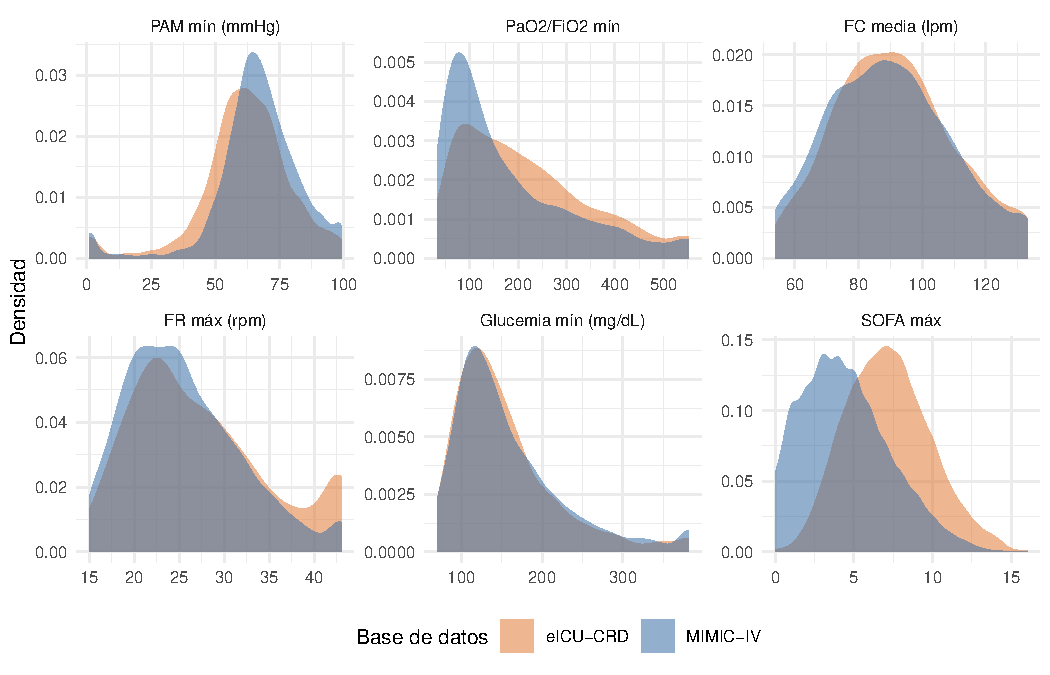
\includegraphics[width=0.9\linewidth,height=\textheight,keepaspectratio]{anexos_files/figure-pdf/fig-densidades-comparadas-1.pdf}

}

\caption{\label{fig-densidades-comparadas}Distribuciones comparadas de
las variables predictoras compartidas entre MIMIC-IV y eICU-CRD (ventana
de observación 0--6 h). Las diferencias de forma reflejan el
desplazamiento de dominio entre la cohorte de desarrollo y la de
validación externa.}

\end{figure}%

Pese a esas diferencias de partida, la dirección de la asociación con el
desenlace se conserva entre cohortes
(Figura~\ref{fig-predictores-desenlace}): tanto en MIMIC-IV como en
eICU-CRD, los pacientes que recibieron noradrenalina presentan una PAM
mínima y un cociente PaO2/FiO2 mínimo inferiores y un SOFA máximo
superior. Esta coherencia en el sentido del efecto es lo que hace
plausible la transferencia de los modelos a la cohorte externa.

\begin{Shaded}
\begin{Highlighting}[]
\NormalTok{variables\_desenlace }\OtherTok{\textless{}{-}} \FunctionTok{c}\NormalTok{(}\StringTok{"map\_min"}\NormalTok{, }\StringTok{"pf\_min"}\NormalTok{, }\StringTok{"sofa\_max"}\NormalTok{)}
\NormalTok{etiquetas\_desenlace }\OtherTok{\textless{}{-}} \FunctionTok{c}\NormalTok{(}
  \StringTok{"PAM mín (mmHg)"}\NormalTok{, }\StringTok{"PaO2/FiO2 mín"}\NormalTok{, }\StringTok{"SOFA máx"}
\NormalTok{)}

\NormalTok{datos\_desenlace }\OtherTok{\textless{}{-}} \FunctionTok{bind\_rows}\NormalTok{(}
\NormalTok{  mimic\_media }\SpecialCharTok{|\textgreater{}}
    \FunctionTok{select}\NormalTok{(base, etiqueta, }\FunctionTok{all\_of}\NormalTok{(variables\_desenlace)),}
\NormalTok{  eicu\_media }\SpecialCharTok{|\textgreater{}}
    \FunctionTok{select}\NormalTok{(base, etiqueta, }\FunctionTok{all\_of}\NormalTok{(variables\_desenlace))}
\NormalTok{) }\SpecialCharTok{|\textgreater{}}
  \FunctionTok{pivot\_longer}\NormalTok{(}
    \FunctionTok{all\_of}\NormalTok{(variables\_desenlace),}
    \AttributeTok{names\_to =} \StringTok{"variable"}\NormalTok{, }\AttributeTok{values\_to =} \StringTok{"valor"}
\NormalTok{  ) }\SpecialCharTok{|\textgreater{}}
  \FunctionTok{mutate}\NormalTok{(}
    \AttributeTok{variable =} \FunctionTok{factor}\NormalTok{(}
\NormalTok{      variable, }\AttributeTok{levels =}\NormalTok{ variables\_desenlace,}
      \AttributeTok{labels =}\NormalTok{ etiquetas\_desenlace}
\NormalTok{    ),}
    \AttributeTok{desenlace =} \FunctionTok{factor}\NormalTok{(}
\NormalTok{      etiqueta, }\AttributeTok{levels =} \FunctionTok{c}\NormalTok{(}\DecValTok{0}\NormalTok{, }\DecValTok{1}\NormalTok{),}
      \AttributeTok{labels =} \FunctionTok{c}\NormalTok{(}\StringTok{"No noradrenalina"}\NormalTok{, }\StringTok{"Noradrenalina"}\NormalTok{)}
\NormalTok{    )}
\NormalTok{  )}

\FunctionTok{ggplot}\NormalTok{(datos\_desenlace,}
       \FunctionTok{aes}\NormalTok{(}\AttributeTok{x =}\NormalTok{ base, }\AttributeTok{y =}\NormalTok{ valor, }\AttributeTok{fill =}\NormalTok{ desenlace)) }\SpecialCharTok{+}
  \FunctionTok{geom\_boxplot}\NormalTok{(}\AttributeTok{outlier.size =} \FloatTok{0.4}\NormalTok{, }\AttributeTok{alpha =} \FloatTok{0.85}\NormalTok{, }\AttributeTok{width =} \FloatTok{0.6}\NormalTok{) }\SpecialCharTok{+}
  \FunctionTok{facet\_wrap}\NormalTok{(}\SpecialCharTok{\textasciitilde{}}\NormalTok{ variable, }\AttributeTok{scales =} \StringTok{"free\_y"}\NormalTok{) }\SpecialCharTok{+}
  \FunctionTok{scale\_fill\_manual}\NormalTok{(}
    \AttributeTok{values =} \FunctionTok{c}\NormalTok{(}\StringTok{"No noradrenalina"} \OtherTok{=} \StringTok{"\#7FB069"}\NormalTok{,}
               \StringTok{"Noradrenalina"} \OtherTok{=} \StringTok{"\#D1495B"}\NormalTok{)}
\NormalTok{  ) }\SpecialCharTok{+}
  \FunctionTok{labs}\NormalTok{(}\AttributeTok{x =} \ConstantTok{NULL}\NormalTok{, }\AttributeTok{y =} \StringTok{"Valor"}\NormalTok{, }\AttributeTok{fill =} \StringTok{"Desenlace"}\NormalTok{) }\SpecialCharTok{+}
  \FunctionTok{theme\_minimal}\NormalTok{(}\AttributeTok{base\_size =} \DecValTok{10}\NormalTok{) }\SpecialCharTok{+}
  \FunctionTok{theme}\NormalTok{(}\AttributeTok{legend.position =} \StringTok{"bottom"}\NormalTok{)}
\end{Highlighting}
\end{Shaded}

\begin{figure}[!h]

\centering{

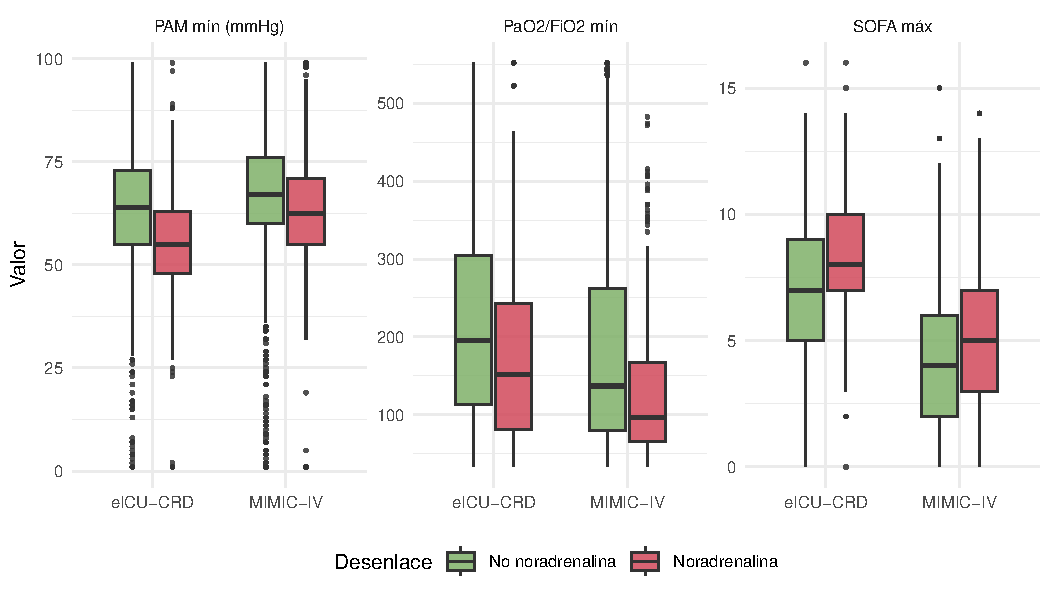
\includegraphics[width=0.9\linewidth,height=\textheight,keepaspectratio]{anexos_files/figure-pdf/fig-predictores-desenlace-1.pdf}

}

\caption{\label{fig-predictores-desenlace}Predictores hemodinámicos y de
gravedad clave según el desenlace (inicio de noradrenalina) en ambas
cohortes (ventana 0--6 h). La dirección de la asociación se mantiene
entre la cohorte de desarrollo y la de validación.}

\end{figure}%

Por último, el tiempo desde el inicio de la ventana de observación hasta
la primera dosis de noradrenalina (Figura~\ref{fig-tiempo-norad}) escala
con el horizonte de predicción. Los valores respetan en todos los casos
los límites inferiores de cada horizonte, lo que confirma la
consistencia del etiquetado entre ambas bases y la ausencia de fugas de
información desde el evento.

\begin{Shaded}
\begin{Highlighting}[]
\NormalTok{seleccionar\_tiempo }\OtherTok{\textless{}{-}} \ControlFlowTok{function}\NormalTok{(marco) \{}
  \FunctionTok{select}\NormalTok{(marco, base, ventana, etiqueta, horas\_hasta\_norad)}
\NormalTok{\}}

\NormalTok{datos\_tiempo }\OtherTok{\textless{}{-}} \FunctionTok{bind\_rows}\NormalTok{(}
  \FunctionTok{seleccionar\_tiempo}\NormalTok{(mimic\_corta),}
  \FunctionTok{seleccionar\_tiempo}\NormalTok{(mimic\_media),}
  \FunctionTok{seleccionar\_tiempo}\NormalTok{(mimic\_larga),}
  \FunctionTok{seleccionar\_tiempo}\NormalTok{(eicu\_corta),}
  \FunctionTok{seleccionar\_tiempo}\NormalTok{(eicu\_media),}
  \FunctionTok{seleccionar\_tiempo}\NormalTok{(eicu\_larga)}
\NormalTok{) }\SpecialCharTok{|\textgreater{}}
  \FunctionTok{filter}\NormalTok{(etiqueta }\SpecialCharTok{==} \DecValTok{1}\NormalTok{, }\SpecialCharTok{!}\FunctionTok{is.na}\NormalTok{(horas\_hasta\_norad)) }\SpecialCharTok{|\textgreater{}}
  \FunctionTok{mutate}\NormalTok{(}
    \AttributeTok{ventana =} \FunctionTok{factor}\NormalTok{(ventana, }\AttributeTok{levels =} \FunctionTok{c}\NormalTok{(}\StringTok{"3 h"}\NormalTok{, }\StringTok{"6 h"}\NormalTok{, }\StringTok{"12 h"}\NormalTok{),}
                     \AttributeTok{labels =} \FunctionTok{c}\NormalTok{(}\StringTok{"Ventana corta (3–12 h)"}\NormalTok{,}
                                \StringTok{"Ventana media (6–24 h)"}\NormalTok{,}
                                \StringTok{"Ventana larga (12–48 h)"}\NormalTok{))}
\NormalTok{  )}

\FunctionTok{ggplot}\NormalTok{(datos\_tiempo,}
       \FunctionTok{aes}\NormalTok{(}\AttributeTok{x =}\NormalTok{ horas\_hasta\_norad, }\AttributeTok{fill =}\NormalTok{ base)) }\SpecialCharTok{+}
  \FunctionTok{geom\_histogram}\NormalTok{(}\AttributeTok{bins =} \DecValTok{25}\NormalTok{, }\AttributeTok{position =} \StringTok{"identity"}\NormalTok{,}
                 \AttributeTok{alpha =} \FloatTok{0.6}\NormalTok{, }\AttributeTok{color =} \StringTok{"white"}\NormalTok{) }\SpecialCharTok{+}
  \FunctionTok{facet\_wrap}\NormalTok{(}\SpecialCharTok{\textasciitilde{}}\NormalTok{ ventana, }\AttributeTok{scales =} \StringTok{"free"}\NormalTok{, }\AttributeTok{ncol =} \DecValTok{3}\NormalTok{) }\SpecialCharTok{+}
  \FunctionTok{scale\_fill\_manual}\NormalTok{(}
    \AttributeTok{values =} \FunctionTok{c}\NormalTok{(}\StringTok{"MIMIC{-}IV"} \OtherTok{=} \StringTok{"\#3B6EA5"}\NormalTok{, }\StringTok{"eICU{-}CRD"} \OtherTok{=} \StringTok{"\#E07B39"}\NormalTok{)}
\NormalTok{  ) }\SpecialCharTok{+}
  \FunctionTok{labs}\NormalTok{(}\AttributeTok{x =} \StringTok{"Horas hasta noradrenalina"}\NormalTok{,}
       \AttributeTok{y =} \StringTok{"Número de pacientes"}\NormalTok{, }\AttributeTok{fill =} \StringTok{"Base de datos"}\NormalTok{) }\SpecialCharTok{+}
  \FunctionTok{theme\_minimal}\NormalTok{(}\AttributeTok{base\_size =} \DecValTok{10}\NormalTok{) }\SpecialCharTok{+}
  \FunctionTok{theme}\NormalTok{(}\AttributeTok{legend.position =} \StringTok{"bottom"}\NormalTok{)}
\end{Highlighting}
\end{Shaded}

\begin{figure}[!h]

\centering{

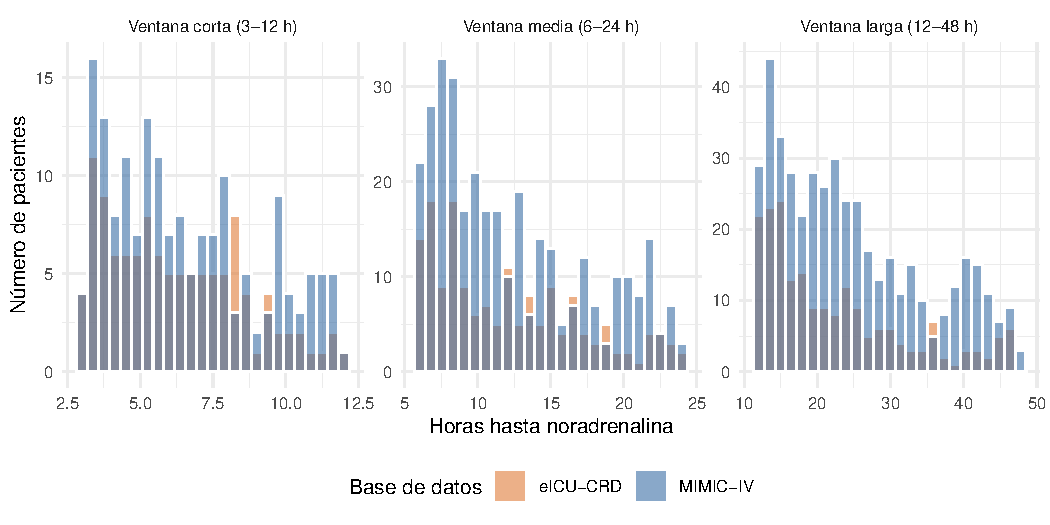
\includegraphics[width=0.9\linewidth,height=\textheight,keepaspectratio]{anexos_files/figure-pdf/fig-tiempo-norad-1.pdf}

}

\caption{\label{fig-tiempo-norad}Tiempo desde el inicio de la ventana de
observación hasta la primera administración de noradrenalina, en los
pacientes con desenlace positivo. Los valores respetan los límites de
cada horizonte de predicción y son consistentes entre ambas bases.}

\end{figure}%

%% ══════════════════════════════════════════════════════
%%  APÉNDICE G – Estudio experimental
%% ══════════════════════════════════════════════════════
\apendice{Estudio experimental}

\section{Cuaderno de trabajo}

El desarrollo de este trabajo no siguió un único experimento cerrado, sino un proceso experimental e iterativo organizado por versiones, en el que
cada fase refinó la definición de la cohorte, el esquema de validación, el conjunto de variables predictoras o el tratamiento de las probabilidades en
función de los resultados de la fase anterior. El repositorio del proyecto conserva esta traza completa: cada carpeta \ruta{Pruebas\ldots} corresponde a
una etapa del cuaderno de trabajo, e incluye tanto los scripts como las salidas (ficheros \texttt{salida\_*.txt}, tablas y figuras) que respaldan las
decisiones tomadas.

Antes de enumerar las fases conviene una advertencia metodológica: las cifras de AUC-ROC no son directamente comparables entre fases tempranas y
finales. A lo largo del proyecto cambiaron simultáneamente la cohorte (prevalencia, criterios de inclusión), el esquema de validación (de una
partición simple a validación cruzada anidada y agrupada por paciente) y el número de variables. Por ello, los descensos de AUC observados al avanzar de
versión no reflejan un empeoramiento del modelo, sino la progresiva eliminación de fuentes de optimismo y la adopción de un protocolo de
evaluación más honesto \cite{kamran2024,rockenschaub2025}.

\begin{table}[htbp]
  \centering
  \caption{Resumen cronológico de las fases experimentales y su correspondencia con el repositorio.}
  \label{tab:cuaderno-fases}
  \resizebox{\textwidth}{!}{%
  \scriptsize
  \begin{tabular}{p{2.0cm} p{3.4cm} p{4.6cm} p{4.6cm}}
    \toprule
    Fase & Carpeta(s) en el repositorio & Foco metodológico & Resultado principal / decisión \\
    \midrule
    I. Cohorte general (6\,h) &
    \ruta{Pruebas cohorte general I} &
    Primeros \textit{baselines} de 5 modelos; partición simple 80/20 y validación cruzada estratificada \emph{no} agrupada; comparación imputación KNN ($k{=}3,5$) frente a caso completo &
    AUC test $\approx 0{,}75$--$0{,}79$; la imputación KNN no aportó mejora. Se descarta KNN. \\
    \addlinespace
    II. Caso completo &
    \ruta{Pruebas cohorte general II}, \ruta{\ldots II SIN MISSINGS} &
    Adopción del análisis de caso completo (sin imputación); reevaluación con KNN $k{=}3,5$ como contraste &
    Diferencias de la imputación frente a no imputar sistemáticamente negativas. Se consolida el enfoque sin imputación. \\
    \addlinespace
    III. Cohorte general ampliada &
    \ruta{Pruebas cohorte general III} &
    Validación cruzada anidada $5\times3$ agrupada por paciente (6 modelos); incorporación de diuresis y nuevas variables &
    AUC $\approx 0{,}68$--$0{,}71$ (CatBoost mejor). Estimación más realista al agrupar por paciente. \\
    \addlinespace
    III-b. Restricción de ventana &
    \ruta{\ldots III restrict ventana} &
    Exigencia de estancia mínima ($>24$\,h) para garantizar que el horizonte de predicción quede cubierto &
    Se evitan falsos negativos por estancias breves (postoperatorios, derivaciones rápidas). \\
    \addlinespace
    IV. Tres ventanas y sepsis &
    \ruta{Pruebas cohorte sepsis IV}, \ruta{\ldots IV ventana 3\_12}, \ruta{\ldots ventana\_12\_48} &
    Construcción definitiva de las cohortes en ventana corta, media y larga; etiquetado de sepsis (Sepsis-3) como variable de subgrupo &
    Cohortes definitivas por ventana; sepsis reservada al análisis diferencial, no como predictor. \\
    \addlinespace
    IV.2. Selección de variables &
    \ruta{Pruebas\_v4\_2}, \ruta{\_corta}, \ruta{\_larga} &
    Correlación de Spearman, agrupamiento jerárquico y eliminación de predictores solapados &
    Reducción de 76 a 25 variables candidatas; correlación residual máxima $|\rho|<0{,}52$. \\
    \addlinespace
    IV.3. Significancia y dirección del efecto &
    \ruta{Pruebas\_v4\_3}, \ruta{\_corta}, \ruta{\_larga} &
    Importancia por permutación, significancia univariante (Mann-Whitney/$\chi^2$ con corrección FDR) y \emph{odds ratio} multivariante &
    Exclusión de variables con dirección de efecto incoherente (p.\,ej. \texttt{gpt\_max} en las tres ventanas). \\
    \addlinespace
    IV.4. Entrenamiento final &
    \ruta{Pruebas\_v4\_4} &
    Validación anidada $5\times3$ de los 6 modelos por ventana, calibración, SHAP y serialización de modelos &
    Selección de modelos candidatos; recalibración efectiva solo de XGBoost (media). \\
    \addlinespace
    V. Validación externa &
    \ruta{Validacion\_externa}, \ruta{eICU} &
    Evaluación en eICU-CRD con IC95\,\% por \textit{bootstrap} y prueba de DeLong aproximada &
    Modelos comparados frente a SOFA; superioridad significativa solo en la ventana larga. \\
    \addlinespace
    VI. Prototipo &
    \ruta{Dashboard} &
    Integración de los modelos en una interfaz Streamlit interpretable &
    Se integran únicamente las ventanas media y larga (XGBoost). \\
    \bottomrule
  \end{tabular}%
  }
\end{table}

\subsection*{Experimentos satisfactorios}

\begin{itemize}
  \item \textbf{Transición a validación anidada agrupada por paciente.} Las primeras fases empleaban una partición simple 80/20 y validación cruzada
  estratificada sin agrupar, lo que permitía que distintas estancias de un mismo paciente cayeran a la vez en entrenamiento y prueba. La adopción de
  \texttt{StratifiedGroupKFold} (bucle externo de 5 particiones, interno de 3) evitó esa fuga de información y produjo estimaciones más honestas, a costa de
  un AUC aparente más bajo \cite{kamran2024}.

  \item \textbf{Restricción de estancia mínima.} Exigir más de 24\,h de estancia (más de 48\,h en la ventana larga) garantizó que el horizonte de
  predicción quedara contenido en el seguimiento disponible, eliminando falsos negativos derivados de estancias demasiado cortas.

  \item \textbf{Reducción del espacio de variables.} El análisis de correlación y agrupamiento jerárquico permitió pasar de 76 a 25 variables
  candidatas conservando la coherencia fisiopatológica y reduciendo la multicolinealidad (correlación residual máxima $|\rho| = 0{,}514$ en la
  ventana corta, $0{,}473$ en la media y $0{,}516$ en la larga).

  \item \textbf{Recalibración de probabilidades.} La evaluación conjunta de curvas \textit{out-of-fold}, ECE y BSS identificó a XGBoost en la ventana
  media como el único modelo que requería recalibración efectiva, resuelta mediante \emph{Platt} regularizado.

  \item \textbf{Validación externa en eICU-CRD.} La transferencia a una cohorte multicéntrica independiente confirmó una discriminación robusta y, en la ventana larga, una mejora estadísticamente
   significativa frente a SOFA \cite{pollard2018,rockenschaub2025}.
\end{itemize}

\subsection*{Experimentos y vías no exitosas}

La inclusión de los resultados negativos es deliberada, ya que orientaron
decisiones de diseño tan relevantes como las positivas:

\begin{itemize}
  \item \textbf{Imputación de datos faltantes mediante KNN.} Probada con $k=3$ y $k=5$ en las fases I y II, no mejoró el rendimiento respecto al
  análisis de caso completo (diferencias sistemáticamente negativas), por lo que se descartó no solo por esto, sino por la dificultad de ordenar 
  el dataset según cada variable para que KNN fuese efectivo, porque había colunas que inicialmene tenían una tasa de,asiado elevada de missings, y finalmente para preservar la fidelidad 
  fisiológica de los datos.

  \item \textbf{Cohorte propia del HUBU.} La heterogeneidad en las estructuras de registro y las barreras de extracción impidieron consolidar la validación
  externa sobre datos del Hospital Universitario de Burgos, que fue sustituida por eICU-CRD \cite{pollard2018}.

  \item \textbf{Reconstrucción de sepsis en eICU-CRD.} No fue posible obtener un indicador de sepsis equivalente al de MIMIC-IV (tabla \texttt{microLab}
  poco poblada y codificación diagnóstica manual no equivalente), de modo que el análisis por subgrupos de sepsis se limitó a MIMIC-IV.

  \item \textbf{Ventana corta en el dashboard.} CatBoost en la ventana corta no superó a SOFA en validación externa, por lo que se excluyó del prototipo,
  que integra solo las ventanas media y larga.

  \item \textbf{Variables con dirección de efecto incoherente.} Se eliminaron
  \texttt{creatinina\_max} y \texttt{gpt\_max} en la ventana corta;
  \texttt{creatinina\_max}, \texttt{ph\_min} y \texttt{gpt\_max} en la media; y
  \texttt{ph\_min}, \texttt{lactato\_max} y \texttt{gpt\_max} en la larga, esta
  última por comportamiento incoherente repetido en las tres ventanas.

  \item \textbf{Regresión logística en la ventana corta.} Tras la selección no conservó variables estadísticamente significativas según la importancia por
  permutación, por lo que no se reportó en esa ventana.
\end{itemize}

\section{Configuración y parametrización de las técnicas}

\subsection*{Esquema de validación}

El rendimiento interno se estimó mediante validación cruzada anidada $5\times3$. El bucle externo dividió las estancias en cinco particiones con
\texttt{StratifiedGroupKFold}, manteniendo la proporción de clases y agrupando todas las estancias de un mismo paciente (\texttt{subject\_id}) en el mismo
\emph{fold} para evitar fuga de información \cite{kamran2024}. El bucle interno (tres particiones) realizó la búsqueda de hiperparámetros con \texttt{GridSearchCV},
optimizando AUC-ROC y con \texttt{refit=True}. Todas las particiones usaron \texttt{shuffle=True} y \texttt{random\_state=42} para reproducibilidad.

\subsection*{Manejo del desbalanceo, escalado y valores extremos}

Con una prevalencia del 10--11\,\% (desbalanceo moderado) se aplicó \texttt{class\_weight='balanced'} en regresión logística, Random Forest y
LightGBM (con \texttt{balanced\_subsample} adicional en Random Forest) y \texttt{scale\_pos\_weight} en XGBoost; CatBoost y Naive Bayes no incorporaron
parámetro de balanceo. El escalado mediante \texttt{RobustScaler} se aplicó únicamente a regresión logística y Naive Bayes, integrado en el
\texttt{Pipeline} para ajustarse exclusivamente sobre el entrenamiento de cada \emph{fold}; los modelos basados en árboles no lo requieren por ser invariantes
a transformaciones monótonas. Los valores extremos se trataron con winsorización al percentil 2 y 98 sobre los estadísticos agregados por estancia \cite{gupta2022mimic}.

\subsection*{Rejillas de hiperparámetros}

La tabla~\ref{tab:rejillas} recoge el espacio de búsqueda explorado para cada algoritmo. Se priorizaron implementaciones maduras y de uso extendido en
problemas clínicos tabulares, interpretables mediante SHAP \cite{lundberg2017}.

\begin{table}[htbp]
  \centering
  \caption{Espacio de hiperparámetros explorado por modelo mediante \texttt{GridSearchCV}.}
  \label{tab:rejillas}
  \resizebox{\textwidth}{!}{%
  \scriptsize
  \begin{tabular}{l p{11.5cm}}
    \toprule
    Modelo & Rejilla de búsqueda (parámetros fijos entre paréntesis) \\
    \midrule
    Regresión logística &
    \texttt{C} $\in\{10^{-4}, 5{\cdot}10^{-4}, 10^{-3}, 5{\cdot}10^{-3}, 10^{-2}, 5{\cdot}10^{-2}, 0{,}1, 0{,}5, 1, 5, 10, 50\}$
    (\texttt{solver=liblinear}, \texttt{class\_weight=balanced}, \texttt{max\_iter=5000}) \\
    \addlinespace
    Random Forest &
    \texttt{n\_estimators} $\in\{300,400,500,600,700,850,1000\}$;
    \texttt{max\_depth} $\in\{$None$,5,10,20,30\}$;
    \texttt{min\_samples\_leaf} $\in\{1,2,5\}$;
    \texttt{max\_features} $\in\{$sqrt$,0{,}3,0{,}5\}$;
    \texttt{class\_weight} $\in\{$balanced, balanced\_subsample$\}$ \\
    \addlinespace
    XGBoost &
    \texttt{n\_estimators} $\in\{300,400,500,600,750,900\}$;
    \texttt{max\_depth} $\in\{3,5,7\}$;
    \texttt{learning\_rate} $\in\{0{,}005,0{,}01,0{,}03,0{,}1\}$;
    \texttt{subsample} $\in\{0{,}6,0{,}8,1{,}0\}$;
    \texttt{colsample\_bytree} $\in\{0{,}6,0{,}8,1{,}0\}$;
    \texttt{reg\_lambda} $\in\{0{,}1,1,10\}$;
    \texttt{scale\_pos\_weight} $\in\{1,5,9\}$
    (\texttt{tree\_method=hist}, \texttt{eval\_metric=auc}) \\
    \addlinespace
    LightGBM &
    \texttt{n\_estimators} $\in\{300,600,1000\}$;
    \texttt{num\_leaves} $\in\{15,31,63\}$;
    \texttt{learning\_rate} $\in\{0{,}005,0{,}01,0{,}03,0{,}1\}$;
    \texttt{min\_child\_samples} $\in\{10,30,60\}$;
    \texttt{reg\_lambda} $\in\{0{,}1,1,10\}$;
    \texttt{subsample} $\in\{0{,}6,0{,}8,1{,}0\}$;
    \texttt{class\_weight} $\in\{$balanced, None$\}$ \\
    \addlinespace
    CatBoost &
    \texttt{iterations} $\in\{500,1000\}$;
    \texttt{depth} $\in\{4,5,6,7\}$;
    \texttt{learning\_rate} $\in\{0{,}01,0{,}03,0{,}05,0{,}1\}$;
    \texttt{l2\_leaf\_reg} $\in\{1,5,15\}$;
    \texttt{bagging\_temperature} $\in\{0,0{,}5,1\}$ \\
    \addlinespace
    Naive Bayes (gaussiano) &
    \texttt{var\_smoothing}: 30 valores en escala logarítmica entre $10^{-12}$ y $10^{-2}$ \\
    \bottomrule
  \end{tabular}%
  }
\end{table}

Como la validación anidada entrena un modelo distinto por \emph{fold}, tras completarla se seleccionó para cada hiperparámetro el \textbf{valor más
frecuente} entre los cinco \emph{folds} externos y se reentrenó el \texttt{Pipeline} sobre el 100\,\% de MIMIC-IV, serializando los modelos en
\texttt{.pkl} con \texttt{joblib} para su reutilización en validación externa y en el dashboard.

\subsection*{Calibración de probabilidades}

Sobre las probabilidades \textit{out-of-fold} se evaluaron tres estrategias de recalibración, entrenando cada calibrador dentro de los \emph{folds} externos para no introducir fuga de información \cite{kamran2024}:

\begin{itemize}
  \item \textbf{Platt sin regularización}: regresión logística con \texttt{C}$=10^{10}$ (sigmoide libre).
  \item \textbf{Platt regularizado}: \texttt{LogisticRegressionCV} con \texttt{Cs=10}, validación interna de 3 particiones y criterio \texttt{neg\_brier\_score}.
  \item \textbf{Regresión isotónica}: ajuste monótono no paramétrico (\texttt{IsotonicRegression} con \texttt{out\_of\_bounds='clip'}).
\end{itemize}

El calibrador final se eligió priorizando el menor ECE entre los métodos con BSS positivo, evitando comprimir las probabilidades hacia la prevalencia;
cuando ningún método cumplía el criterio, se conservó el modelo sin calibrar.

\subsection*{Interpretabilidad y métricas}

La interpretabilidad \emph{post-hoc} se abordó con valores SHAP \cite{lundberg2017}, empleando \texttt{TreeExplainer} en los modelos de
árboles, \texttt{LinearExplainer} en la regresión logística y \texttt{KernelExplainer} en Naive Bayes, con visualización mediante diagramas
\textit{beeswarm}. SHAP no se empleó para seleccionar variables, sino como capa de auditoría de la coherencia fisiopatológica.

La evaluación combinó discriminación (AUC-ROC y AUC-PR), rendimiento probabilístico (\textit{Brier score}, \textit{Brier Skill Score} y
\textit{LogLoss}) y calibración (\textit{Expected Calibration Error}, ECE, con 10 intervalos). El BSS se define respecto a un modelo nulo que predice siempre
la prevalencia:
\[
  \mathrm{BSS} = 1 - \frac{\mathrm{Brier}_{\text{modelo}}}{\mathrm{Brier}_{\text{nulo}}},
\]
de modo que un BSS positivo indica mejora sobre la predicción trivial. La
significancia univariante empleó la corrección de Benjamini-Hochberg
($\mathrm{FDR}\ q<0{,}05$) \cite{benjamini1995}.

\section{Detalle de resultados}

\subsection*{Variables retenidas por cada modelo y ventana}

La tabla~\ref{tab:vars-finales} recoge el subconjunto de predictores seleccionado para cada combinación de modelo y ventana, resultado del proceso de selección descrito en la sección anterior.

\begin{table}[htbp]
  \centering
  \caption{Variables predictoras retenidas por cada modelo en cada ventana temporal.}
  \label{tab:vars-finales}
  \resizebox{\textwidth}{!}{%
  \scriptsize
  \begin{tabular}{l l p{10.5cm}}
    \toprule
    Ventana & Modelo & Variables \\
    \midrule
    \multirow{5}{*}{Corta (3--12\,h)}
      & RF   & \texttt{temp\_min}, \texttt{rr\_max} \\
      & XGB  & \texttt{pf\_min}, \texttt{map\_min}, \texttt{diuresis\_ml\_kg\_3h}, \texttt{sofa\_max} \\
      & LGBM & \texttt{map\_min}, \texttt{pf\_min}, \texttt{sofa\_max} \\
      & CAT  & \texttt{map\_min}, \texttt{pf\_min}, \texttt{sofa\_max}, \texttt{tp\_max} \\
      & NB   & \texttt{map\_min}, \texttt{temp\_min}, \texttt{spo2\_min} \\
    \midrule
    \multirow{6}{*}{Media (6--24\,h)}
      & LR   & \texttt{pf\_min}, \texttt{diuresis\_ml\_kg\_6h}, \texttt{rr\_max}, \texttt{sofa\_max}, \texttt{hr\_media}, \texttt{ventilacion\_invasiva\_6h} \\
      & RF   & \texttt{pf\_min}, \texttt{map\_min}, \texttt{diuresis\_ml\_kg\_6h}, \texttt{rr\_max}, \texttt{spo2\_min}, \texttt{hr\_media}, \texttt{glucemia\_min}, \texttt{ventilacion\_invasiva\_6h} \\
      & XGB  & \texttt{pf\_min}, \texttt{map\_min}, \texttt{diuresis\_ml\_kg\_6h}, \texttt{hr\_media}, \texttt{sofa\_max}, \texttt{ventilacion\_invasiva\_6h} \\
      & LGBM & \texttt{map\_min}, \texttt{pf\_min}, \texttt{diuresis\_ml\_kg\_6h}, \texttt{spo2\_min}, \texttt{ventilacion\_invasiva\_6h} \\
      & CAT  & \texttt{map\_min}, \texttt{pf\_min}, \texttt{diuresis\_ml\_kg\_6h}, \texttt{hr\_media}, \texttt{rr\_max}, \texttt{glucemia\_min}, \texttt{ventilacion\_invasiva\_6h} \\
      & NB   & \texttt{pf\_min}, \texttt{diuresis\_ml\_kg\_6h}, \texttt{rr\_max}, \texttt{lactato\_max}, \texttt{sofa\_max}, \texttt{hr\_media}, \texttt{ventilacion\_invasiva\_6h} \\
    \midrule
    \multirow{6}{*}{Larga (12--48\,h)}
      & LR   & \texttt{temp\_min}, \texttt{pf\_min}, \texttt{spo2\_min}, \texttt{bicarbonato\_min}, \texttt{rr\_max}, \texttt{map\_min} \\
      & RF   & \texttt{temp\_min}, \texttt{spo2\_min}, \texttt{bicarbonato\_min}, \texttt{rr\_max}, \texttt{map\_min}, \texttt{glucemia\_min}, \texttt{sofa\_max}, \texttt{diuresis\_ml\_kg\_12h}, \texttt{bilirrubina\_media} \\
      & XGB  & \texttt{temp\_min}, \texttt{pf\_min}, \texttt{spo2\_min}, \texttt{bicarbonato\_min}, \texttt{map\_min}, \texttt{glucemia\_min}, \texttt{sofa\_max} \\
      & LGBM & \texttt{temp\_min}, \texttt{spo2\_min}, \texttt{bicarbonato\_min}, \texttt{rr\_max}, \texttt{glucemia\_min}, \texttt{sofa\_max}, \texttt{diuresis\_ml\_kg\_12h}, \texttt{map\_min}, \texttt{pf\_min} \\
      & CAT  & \texttt{pf\_min}, \texttt{temp\_min}, \texttt{diuresis\_ml\_kg\_12h}, \texttt{bicarbonato\_min}, \texttt{rr\_max}, \texttt{glucemia\_min} \\
      & NB   & \texttt{temp\_min}, \texttt{pf\_min}, \texttt{spo2\_min}, \texttt{rr\_max}, \texttt{map\_min} \\
    \bottomrule
  \end{tabular}%
  }
\end{table}

\subsection*{Validación interna completa (MIMIC-IV)}

La tabla~\ref{tab:interna-completa} recoge el rendimiento de los dieciocho modelos evaluados mediante validación cruzada anidada (media $\pm$ desviación
estándar entre \emph{folds} externos). En la ventana corta no aparece la regresión logística por no conservar variables significativas; en XGBoost de la
ventana media, el BSS y el ECE no se reportan en su versión sin calibrar por inestabilidad numérica de la calibración previa al ajuste.

\begin{table}[htbp]
  \centering
  \caption{Rendimiento interno de todos los modelos en MIMIC-IV (validación cruzada anidada).}
  \label{tab:interna-completa}
  \resizebox{\textwidth}{!}{%
  \scriptsize
  \setlength{\tabcolsep}{4pt}
  \begin{tabular}{l l c c c c c c c}
    \toprule
    Vent. & Modelo & Vars & AUC-ROC & AUC-PR & Brier & BSS & ECE & LogLoss \\
    \midrule
    Corta & RF   & 2 & $0{,}592 \pm 0{,}054$ & $0{,}177 \pm 0{,}051$ & $0{,}194 \pm 0{,}008$ & $-1{,}097 \pm 0{,}099$ & $0{,}308 \pm 0{,}007$ & $0{,}577 \pm 0{,}016$ \\
    Corta & XGB  & 4 & $0{,}623 \pm 0{,}035$ & $0{,}164 \pm 0{,}019$ & $0{,}104 \pm 0{,}026$ & $-0{,}127 \pm 0{,}283$ & $0{,}065 \pm 0{,}095$ & $0{,}359 \pm 0{,}068$ \\
    Corta & LGBM & 3 & $0{,}570 \pm 0{,}044$ & $0{,}125 \pm 0{,}015$ & $0{,}146 \pm 0{,}063$ & $-0{,}580 \pm 0{,}695$ & $0{,}159 \pm 0{,}151$ & $0{,}456 \pm 0{,}144$ \\
    Corta & CAT  & 4 & $0{,}623 \pm 0{,}043$ & $0{,}166 \pm 0{,}012$ & $0{,}091 \pm 0{,}001$ & $0{,}012 \pm 0{,}010$ & $0{,}020 \pm 0{,}006$ & $0{,}325 \pm 0{,}005$ \\
    Corta & NB   & 3 & $0{,}640 \pm 0{,}037$ & $0{,}181 \pm 0{,}025$ & $0{,}095 \pm 0{,}003$ & $-0{,}024 \pm 0{,}025$ & $0{,}032 \pm 0{,}004$ & $0{,}332 \pm 0{,}010$ \\
    \midrule
    Media & LR        & 6 & $0{,}688 \pm 0{,}010$ & $0{,}222 \pm 0{,}031$ & $0{,}224 \pm 0{,}005$ & $-1{,}421 \pm 0{,}049$ & $0{,}353 \pm 0{,}003$ & $0{,}636 \pm 0{,}010$ \\
    Media & RF        & 8 & $0{,}690 \pm 0{,}023$ & $0{,}225 \pm 0{,}022$ & $0{,}180 \pm 0{,}004$ & $-0{,}946 \pm 0{,}042$ & $0{,}295 \pm 0{,}004$ & $0{,}543 \pm 0{,}008$ \\
    Media & XGB       & 6 & $0{,}678 \pm 0{,}011$ & $0{,}215 \pm 0{,}029$ & $0{,}160 \pm 0{,}058$ & --- & --- & $0{,}488 \pm 0{,}141$ \\
    Media & XGB cal.  & 6 & $0{,}683 \pm 0{,}010$ & $0{,}217 \pm 0{,}029$ & $0{,}090 \pm 0{,}002$ & $0{,}026 \pm 0{,}023$ & $0{,}036 \pm 0{,}005$ & $0{,}320 \pm 0{,}004$ \\
    Media & LGBM      & 5 & $0{,}660 \pm 0{,}015$ & $0{,}193 \pm 0{,}025$ & $0{,}131 \pm 0{,}051$ & $-0{,}420 \pm 0{,}547$ & $0{,}130 \pm 0{,}140$ & $0{,}418 \pm 0{,}124$ \\
    Media & CAT       & 7 & $0{,}696 \pm 0{,}015$ & $0{,}223 \pm 0{,}030$ & $0{,}088 \pm 0{,}001$ & $0{,}050 \pm 0{,}014$ & $0{,}017 \pm 0{,}011$ & $0{,}309 \pm 0{,}003$ \\
    Media & NB        & 7 & $0{,}676 \pm 0{,}018$ & $0{,}193 \pm 0{,}029$ & $0{,}105 \pm 0{,}006$ & $-0{,}136 \pm 0{,}072$ & $0{,}056 \pm 0{,}010$ & $0{,}363 \pm 0{,}023$ \\
    \midrule
    Larga & LR   & 6 & $0{,}642 \pm 0{,}035$ & $0{,}185 \pm 0{,}025$ & $0{,}240 \pm 0{,}003$ & $-1{,}421 \pm 0{,}030$ & $0{,}373 \pm 0{,}008$ & $0{,}673 \pm 0{,}006$ \\
    Larga & RF   & 9 & $0{,}632 \pm 0{,}018$ & $0{,}196 \pm 0{,}011$ & $0{,}165 \pm 0{,}043$ & $-0{,}668 \pm 0{,}437$ & $0{,}238 \pm 0{,}099$ & $0{,}508 \pm 0{,}102$ \\
    Larga & XGB  & 7 & $0{,}648 \pm 0{,}042$ & $0{,}187 \pm 0{,}033$ & $0{,}109 \pm 0{,}025$ & $-0{,}103 \pm 0{,}251$ & $0{,}064 \pm 0{,}090$ & $0{,}371 \pm 0{,}065$ \\
    Larga & LGBM & 9 & $0{,}632 \pm 0{,}031$ & $0{,}185 \pm 0{,}037$ & $0{,}143 \pm 0{,}056$ & $-0{,}444 \pm 0{,}562$ & $0{,}141 \pm 0{,}156$ & $0{,}450 \pm 0{,}132$ \\
    Larga & CAT  & 6 & $0{,}645 \pm 0{,}030$ & $0{,}201 \pm 0{,}021$ & $0{,}096 \pm 0{,}001$ & $0{,}028 \pm 0{,}012$ & $0{,}014 \pm 0{,}008$ & $0{,}337 \pm 0{,}005$ \\
    Larga & NB   & 5 & $0{,}624 \pm 0{,}034$ & $0{,}170 \pm 0{,}020$ & $0{,}104 \pm 0{,}005$ & $-0{,}052 \pm 0{,}053$ & $0{,}036 \pm 0{,}012$ & $0{,}361 \pm 0{,}018$ \\
    \bottomrule
  \end{tabular}%
  }
\end{table}

\subsection*{Hiperparámetros finales de los modelos principales}

La tabla~\ref{tab:hiperparametros-finales} documenta los hiperparámetros efectivamente serializados para los modelos seleccionados como principales en cada ventana, obtenidos por el 
procedimiento de valor más frecuente entre \emph{folds} y reentrenamiento sobre la cohorte interna completa.

\begin{table}[htbp]
  \centering
  \caption{Hiperparámetros finales de los modelos principales por ventana.}
  \label{tab:hiperparametros-finales}
  \resizebox{\textwidth}{!}{%
  \scriptsize
  \begin{tabular}{l l p{9.5cm}}
    \toprule
    Ventana & Modelo & Hiperparámetros \\
    \midrule
    Corta (3--12\,h) & CatBoost &
    \texttt{iterations}=500, \texttt{depth}=4, \texttt{learning\_rate}=0{,}01, \texttt{l2\_leaf\_reg}=15, \texttt{bagging\_temperature}=0 \\
    \addlinespace
    Media (6--24\,h) & XGBoost (base del calibrado) &
    \texttt{n\_estimators}=300, \texttt{max\_depth}=3, \texttt{learning\_rate}=0{,}01, \texttt{subsample}=0{,}6, \texttt{colsample\_bytree}=1{,}0, \texttt{reg\_lambda}=10, \texttt{scale\_pos\_weight}=9 \\
    \addlinespace
    Media (6--24\,h) & CatBoost &
    \texttt{iterations}=500, \texttt{depth}=4, \texttt{learning\_rate}=0{,}01, \texttt{l2\_leaf\_reg}=5, \texttt{bagging\_temperature}=0 \\
    \addlinespace
    Larga (12--48\,h) & XGBoost &
    \texttt{n\_estimators}=300, \texttt{max\_depth}=3, \texttt{learning\_rate}=0{,}005, \texttt{subsample}=0{,}6, \texttt{colsample\_bytree}=0{,}8, \texttt{reg\_lambda}=10, \texttt{scale\_pos\_weight}=1 \\
    \addlinespace
    Larga (12--48\,h) & CatBoost &
    \texttt{iterations}=500, \texttt{depth}=4, \texttt{learning\_rate}=0{,}01, \texttt{l2\_leaf\_reg}=15, \texttt{bagging\_temperature}=0 \\
    \bottomrule
  \end{tabular}%
  }
\end{table}

El modelo de la ventana media se recalibró mediante \emph{Platt} regularizado sobre la salida de XGBoost; el resto de modelos principales se conservó sin recalibración por no cumplir el criterio
de mejora (BSS positivo con menor ECE).

\subsection*{Análisis por subgrupos según presencia de sepsis (MIMIC-IV)}

La tabla~\ref{tab:subgrupos-sepsis} recoge el rendimiento de los modelos seleccionados por ventana, estratificado en cohorte global, pacientes con sepsis (Sepsis-3) y sin sepsis, calculado 
mediante predicciones \textit{out-of-fold} y empleando SOFA como referencia clínica de comparación \cite{singer2016}.

\begin{table}[htbp]
  \centering
  \caption{Rendimiento por subgrupos de sepsis en MIMIC-IV (predicciones \textit{out-of-fold}).}
  \label{tab:subgrupos-sepsis}
  \resizebox{\textwidth}{!}{%
  \scriptsize
  \begin{tabular}{l l c c c c c}
    \toprule
    Ventana & Subgrupo / modelo & $N$ & AUC-ROC & AUC-PR & BSS & ECE \\
    \midrule
    \multirow{4}{*}{Corta (CatBoost)}
      & Global       & 1667 & $0{,}617$ & $0{,}151$ & $+0{,}012$ & $0{,}009$ \\
      & Sépticos     &  461 & $0{,}622$ & $0{,}173$ & $+0{,}004$ & $0{,}021$ \\
      & No sépticos  & 1206 & $0{,}605$ & $0{,}152$ & $+0{,}013$ & $0{,}012$ \\
      & SOFA (global)& 1667 & $0{,}581$ & $0{,}132$ & --- & --- \\
    \midrule
    \multirow{4}{*}{Media (XGBoost cal.)}
      & Global       & 3282 & $0{,}680$ & $0{,}208$ & $+0{,}028$ & $0{,}033$ \\
      & Sépticos     &  993 & $0{,}694$ & $0{,}287$ & $+0{,}064$ & $0{,}028$ \\
      & No sépticos  & 2289 & $0{,}667$ & $0{,}173$ & $+0{,}003$ & $0{,}036$ \\
      & SOFA (global)& 3282 & $0{,}606$ & $0{,}147$ & --- & --- \\
    \midrule
    \multirow{4}{*}{Larga (XGBoost)}
      & Global       & 4088 & $0{,}642$ & $0{,}170$ & $+0{,}021$ & $0{,}017$ \\
      & Sépticos     & 1343 & $0{,}650$ & $0{,}209$ & $+0{,}018$ & $0{,}030$ \\
      & No sépticos  & 2745 & $0{,}630$ & $0{,}150$ & $+0{,}017$ & $0{,}011$ \\
      & SOFA (global)& 4088 & $0{,}588$ & $0{,}149$ & --- & --- \\
    \bottomrule
  \end{tabular}%
  }
\end{table}

El rendimiento discriminativo fue sistemáticamente superior en el subgrupo séptico, de forma más marcada en la ventana media (AUC-ROC $0{,}694$ frente a
$0{,}667$ en no sépticos), aunque los modelos mantuvieron capacidad discriminativa por encima del azar también en pacientes sin sospecha de sepsis.

\subsection*{Validación externa sobre eICU-CRD}

Las tablas~\ref{tab:externa-discriminacion} y~\ref{tab:externa-probabilistica} recogen, respectivamente, la discriminación frente a SOFA y las métricas
probabilísticas y de calibración en la cohorte externa, con intervalos de confianza al 95\,\% calculados mediante \textit{bootstrap} (1000 repeticiones)
y diferencia de AUC contrastada mediante una prueba de DeLong aproximada por \textit{bootstrap}.

\begin{table}[htbp]
  \centering
  \caption{Validación externa (eICU-CRD): discriminación de cada modelo frente a SOFA como predictor aislado.}
  \label{tab:externa-discriminacion}
  \resizebox{\textwidth}{!}{%
  \scriptsize
  \begin{tabular}{l c c c c c c c}
    \toprule
    Modelo / ventana & $N$ & Prev. (\%) & AUC modelo & AUC SOFA & $\Delta$AUC & $p$ DeLong & AUC-PR \\
    \midrule
    Corta 3--12\,h (CatBoost)      &  789 & 14{,}4 & $0{,}630$ $[0{,}572$--$0{,}689]$ & $0{,}642$ $[0{,}588$--$0{,}692]$ & $-0{,}010$ & $0{,}698$  & $0{,}240$ $[0{,}187$--$0{,}315]$ \\
    Media 6--24\,h (XGBoost cal.)  & 1396 & 11{,}9 & $0{,}662$ $[0{,}618$--$0{,}708]$ & $0{,}663$ $[0{,}620$--$0{,}706]$ & $-0{,}001$ & $0{,}978$  & $0{,}228$ $[0{,}180$--$0{,}295]$ \\
    Media 6--24\,h (CatBoost)      & 1396 & 11{,}9 & $0{,}669$ $[0{,}627$--$0{,}714]$ & $0{,}663$ $[0{,}620$--$0{,}706]$ & $+0{,}006$ & $0{,}803$  & $0{,}238$ $[0{,}189$--$0{,}311]$ \\
    Larga 12--48\,h (XGBoost)      & 2030 &  9{,}8 & $0{,}658$ $[0{,}620$--$0{,}694]$ & $0{,}590$ $[0{,}548$--$0{,}631]$ & $+0{,}068$ & $<0{,}001$ & $0{,}164$ $[0{,}132$--$0{,}208]$ \\
    Larga 12--48\,h (CatBoost)     & 2030 &  9{,}8 & $0{,}653$ $[0{,}616$--$0{,}691]$ & $0{,}590$ $[0{,}548$--$0{,}631]$ & $+0{,}064$ & $0{,}003$  & $0{,}152$ $[0{,}125$--$0{,}191]$ \\
    \bottomrule
  \end{tabular}%
  }
\end{table}

\begin{table}[htbp]
  \centering
  \caption{Validación externa (eICU-CRD): métricas probabilísticas y de calibración de cada modelo.}
  \label{tab:externa-probabilistica}
  \resizebox{\textwidth}{!}{%
  \scriptsize
  \begin{tabular}{l c c c c c}
    \toprule
    Modelo / ventana & $N$ & Prev. (\%) & Brier & BSS & ECE \\
    \midrule
    Corta 3--12\,h (CatBoost)      &  789 & 14{,}4 & $0{,}121$ $[0{,}102$--$0{,}140]$ & $0{,}025$ $[-0{,}001$--$0{,}049]$ & $0{,}029$ $[0{,}011$--$0{,}058]$ \\
    Media 6--24\,h (XGBoost cal.)  & 1396 & 11{,}9 & $0{,}101$ $[0{,}088$--$0{,}114]$ & $0{,}040$ $[0{,}017$--$0{,}066]$  & $0{,}016$ $[0{,}007$--$0{,}033]$ \\
    Media 6--24\,h (CatBoost)      & 1396 & 11{,}9 & $0{,}100$ $[0{,}087$--$0{,}114]$ & $0{,}046$ $[0{,}020$--$0{,}073]$  & $0{,}017$ $[0{,}009$--$0{,}035]$ \\
    Larga 12--48\,h (XGBoost)      & 2030 &  9{,}8 & $0{,}087$ $[0{,}077$--$0{,}097]$ & $0{,}019$ $[0{,}003$--$0{,}031]$  & $0{,}021$ $[0{,}011$--$0{,}033]$ \\
    Larga 12--48\,h (CatBoost)     & 2030 &  9{,}8 & $0{,}087$ $[0{,}077$--$0{,}098]$ & $0{,}019$ $[0{,}002$--$0{,}034]$  & $0{,}013$ $[0{,}007$--$0{,}027]$ \\
    \bottomrule
  \end{tabular}%
  }
\end{table}

En la ventana larga, XGBoost y CatBoost superaron a SOFA de forma estadísticamente significativa ($\Delta\mathrm{AUC}=+0{,}068$, $p<0{,}001$ y
$+0{,}064$, $p=0{,}003$); en la media igualaron prácticamente a SOFA y en la corta no aportaron ventaja. La degradación entre validación interna y externa
es coherente con lo esperable en modelos clínicos transhospitalarios \cite{rockenschaub2025}.

\subsection*{Encuesta de satisfacción del prototipo}

La encuesta sobre el prototipo de dashboard, cumplimentada por ocho facultativos del servicio de Medicina Intensiva del HUBU en una escala de 1 a
10, arrojó puntuaciones medias de \textbf{8,87} en entendimiento de la interfaz, \textbf{8,50} en explicabilidad y \textbf{8,00} en utilidad clínica
potencial. Estos resultados, exploratorios por el tamaño reducido de la muestra, sugieren que el prototipo se percibió como comprensible y potencialmente útil.

\subsection*{Material gráfico complementario}

La figura~\ref{fig:permutation} resume la importancia por permutación empleada
como filtro de selección
 
\begin{figure}[htbp]
  \centering
  \begin{subfigure}[t]{0.32\textwidth}\centering
    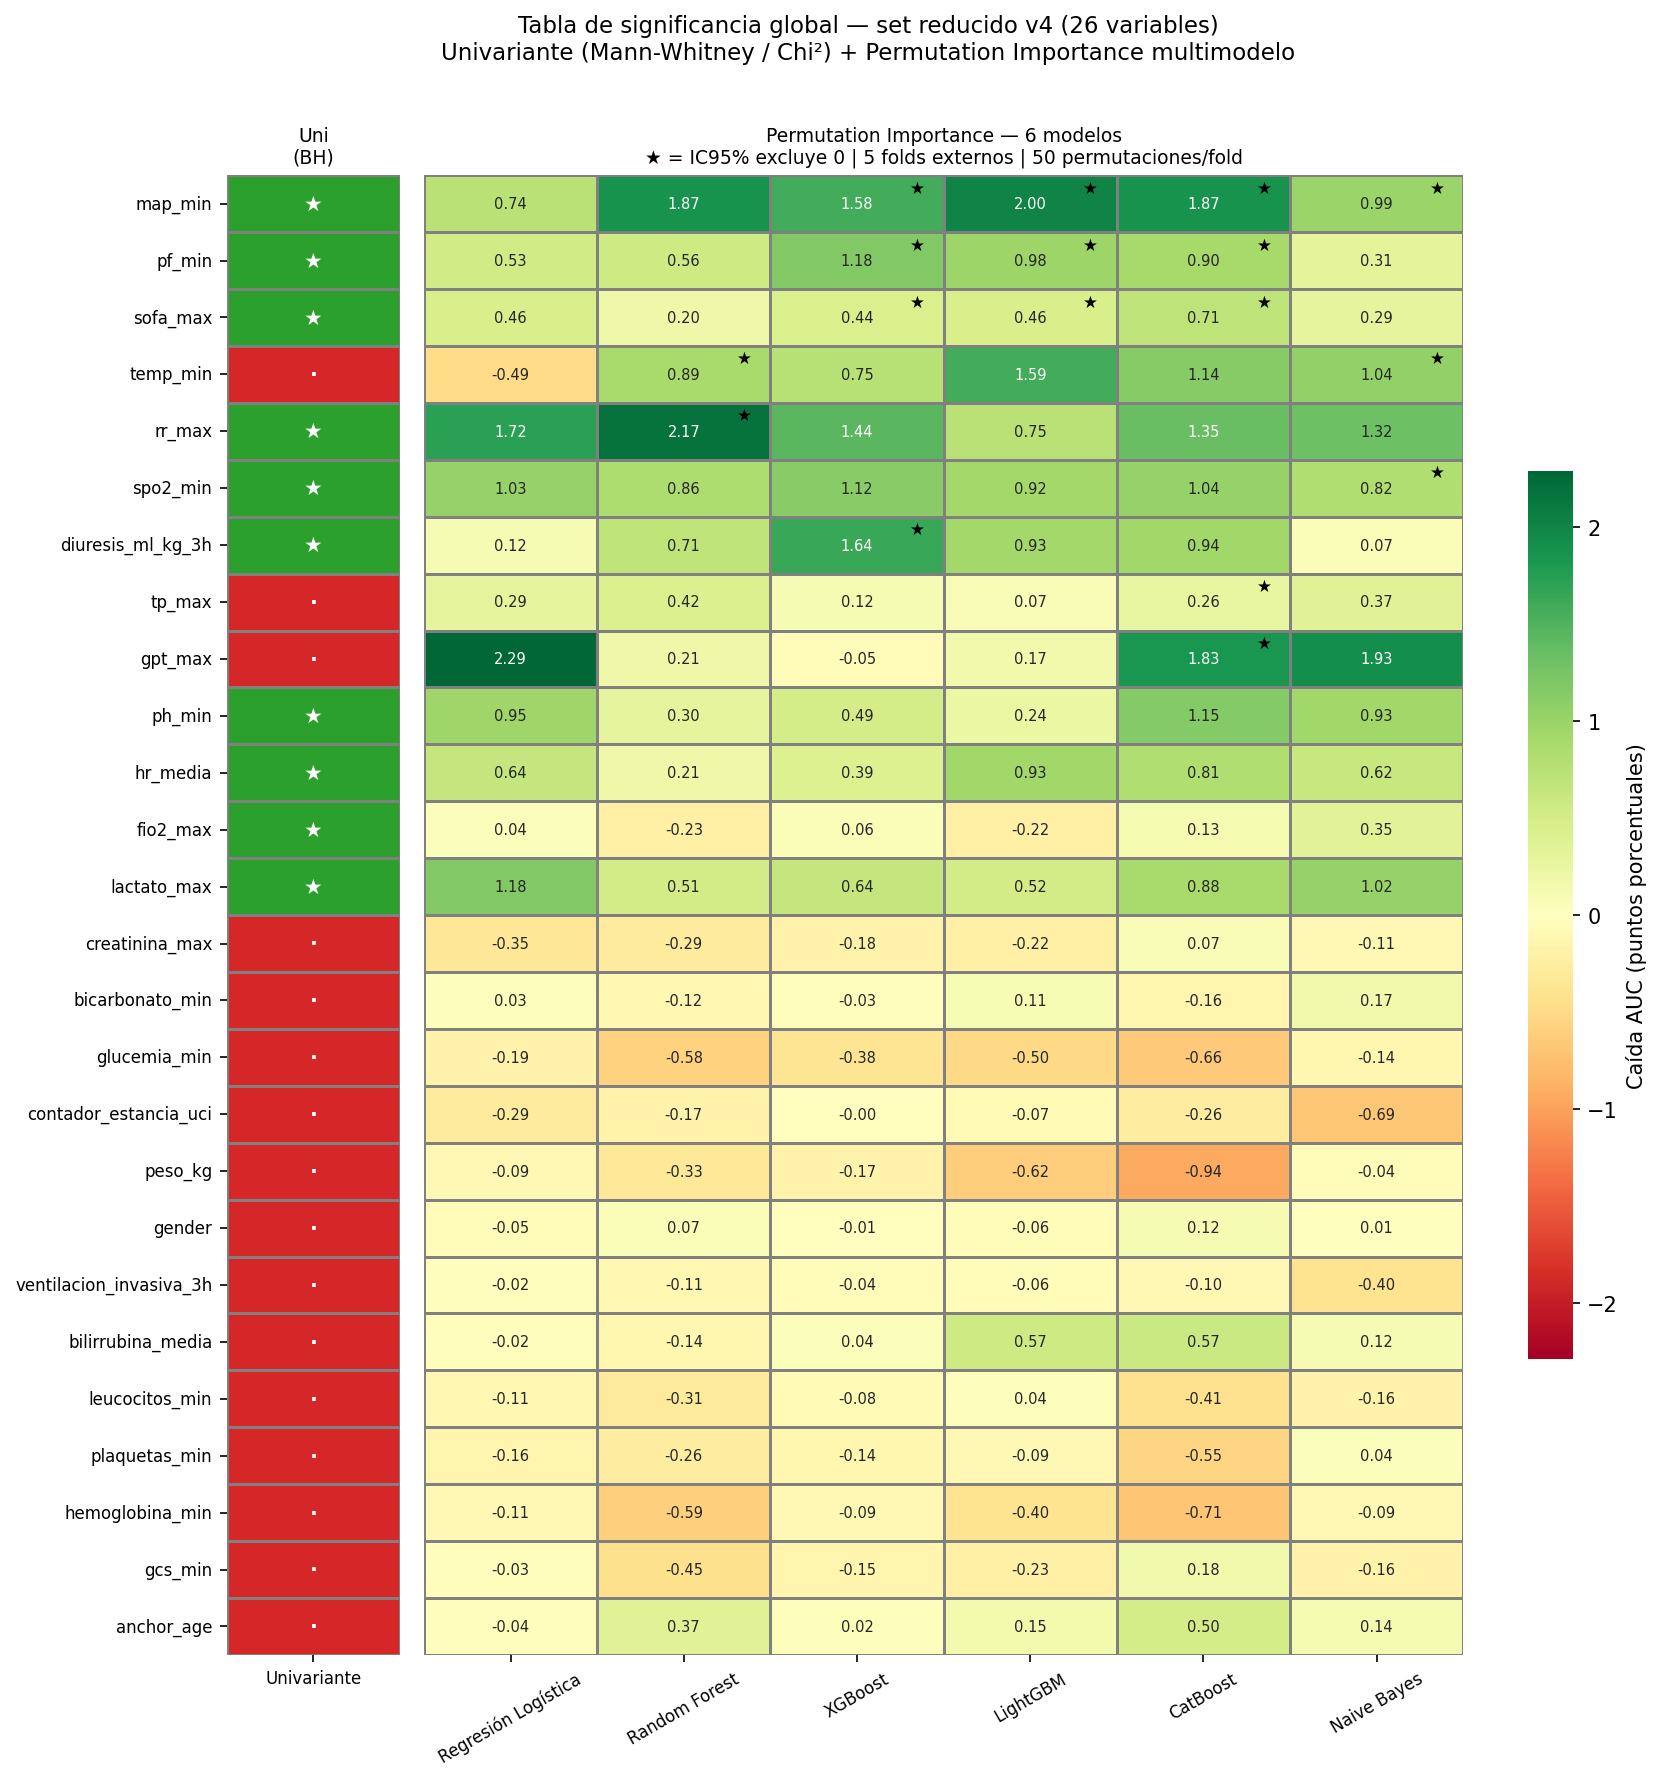
\includegraphics[width=\linewidth]{img/significancia_global_v4p.png}
    \caption{Corta}
  \end{subfigure}\hfill
  \begin{subfigure}[t]{0.32\textwidth}\centering
    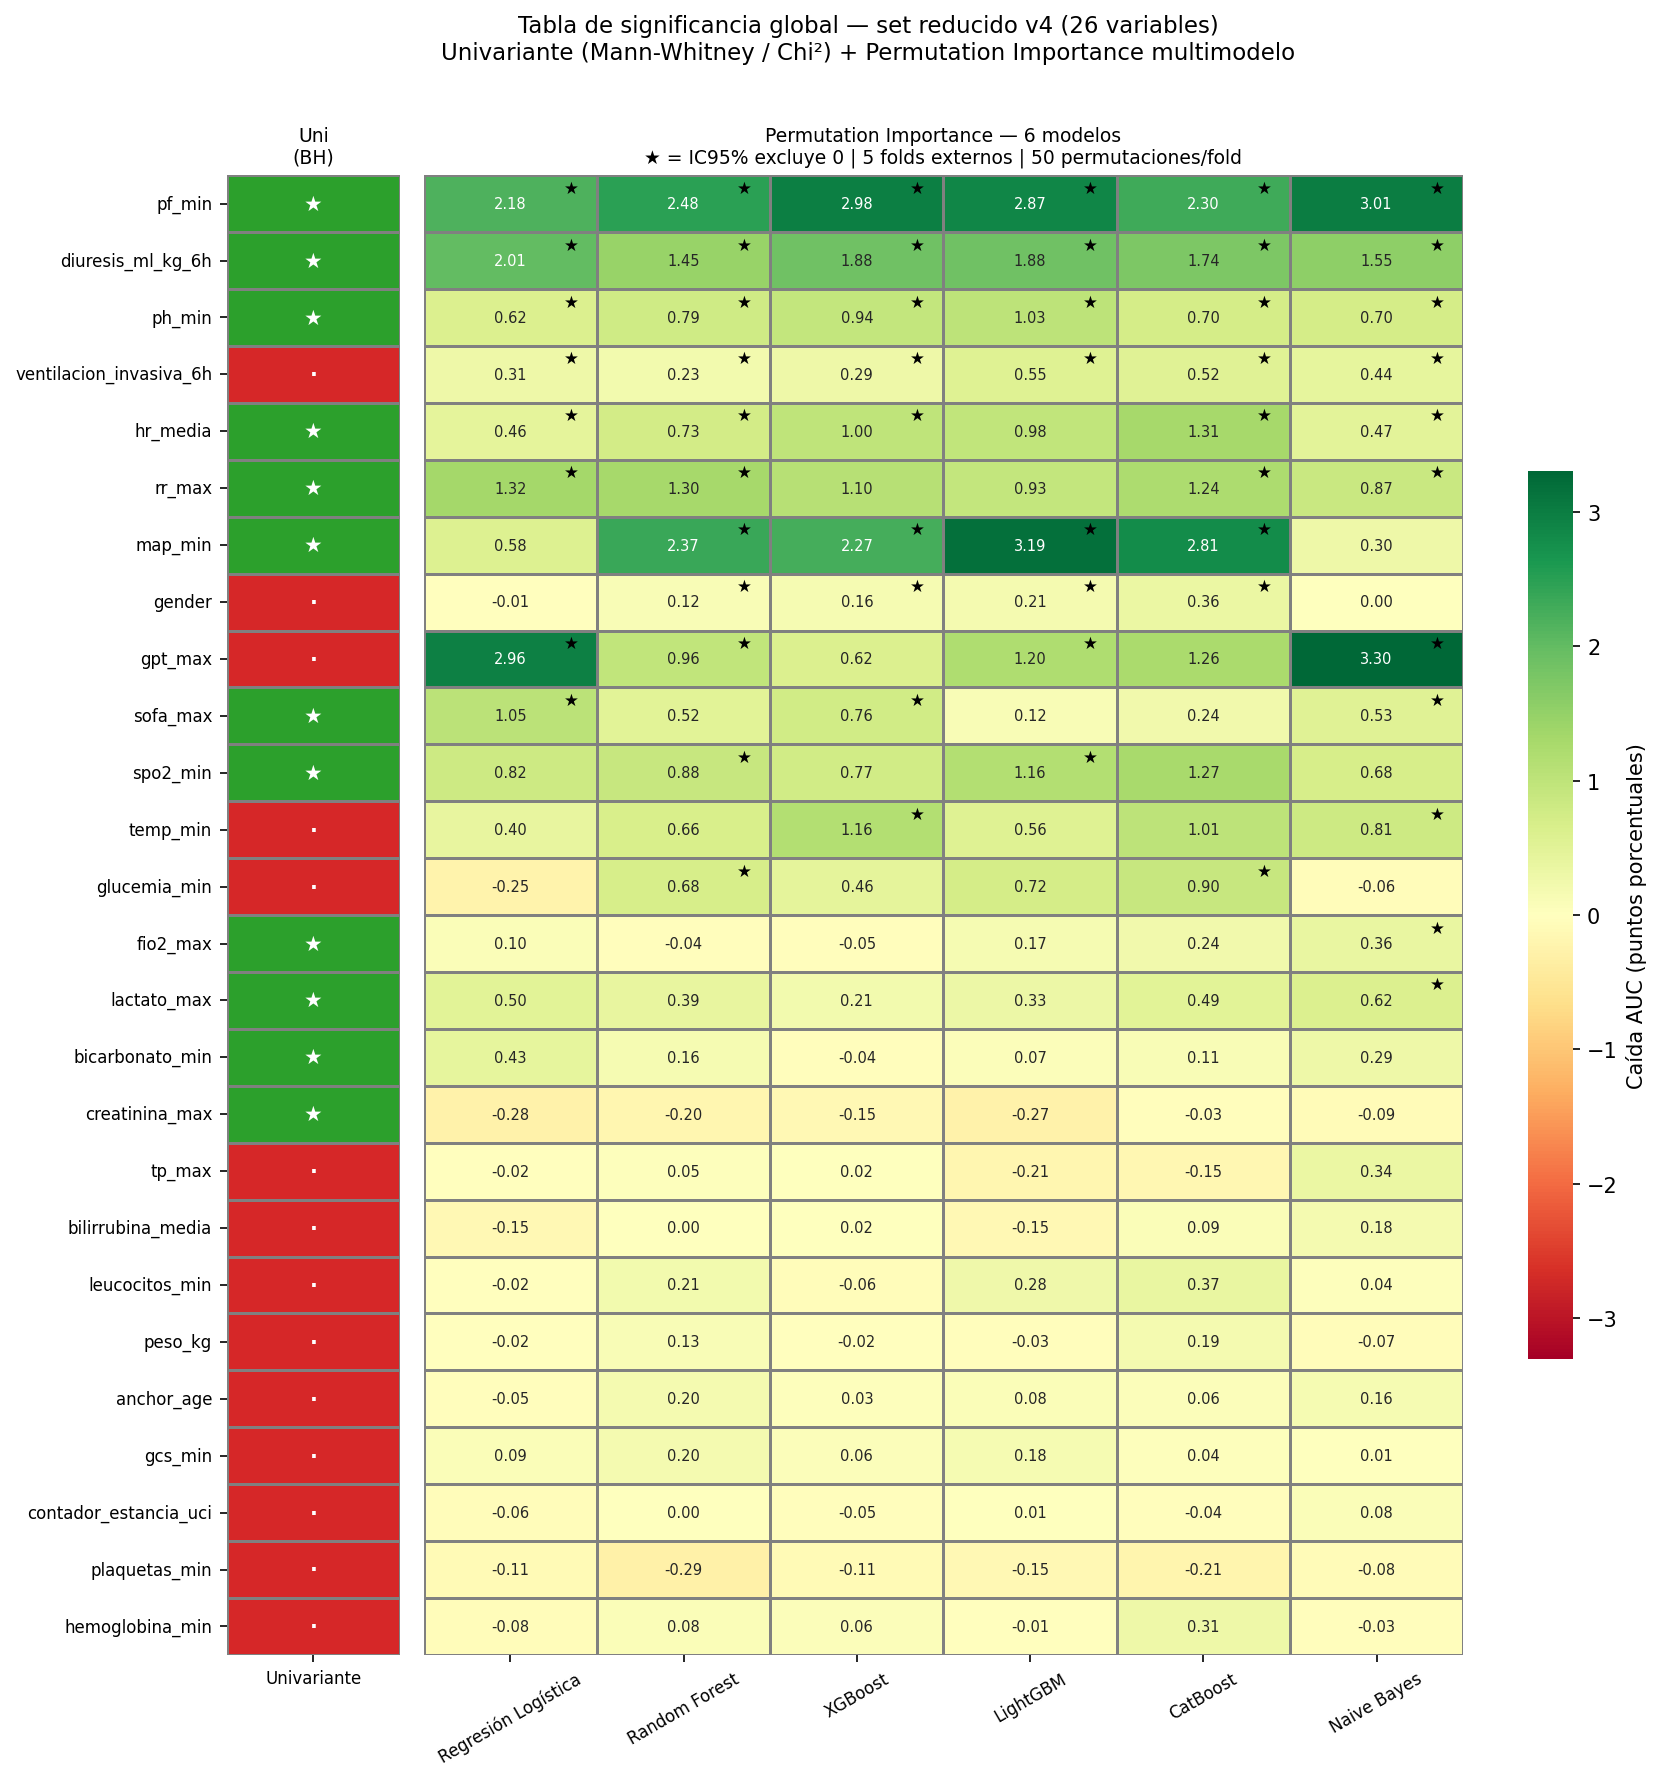
\includegraphics[width=\linewidth]{img/significancia_global_v4.png}
    \caption{Media}
  \end{subfigure}\hfill
  \begin{subfigure}[t]{0.32\textwidth}\centering
    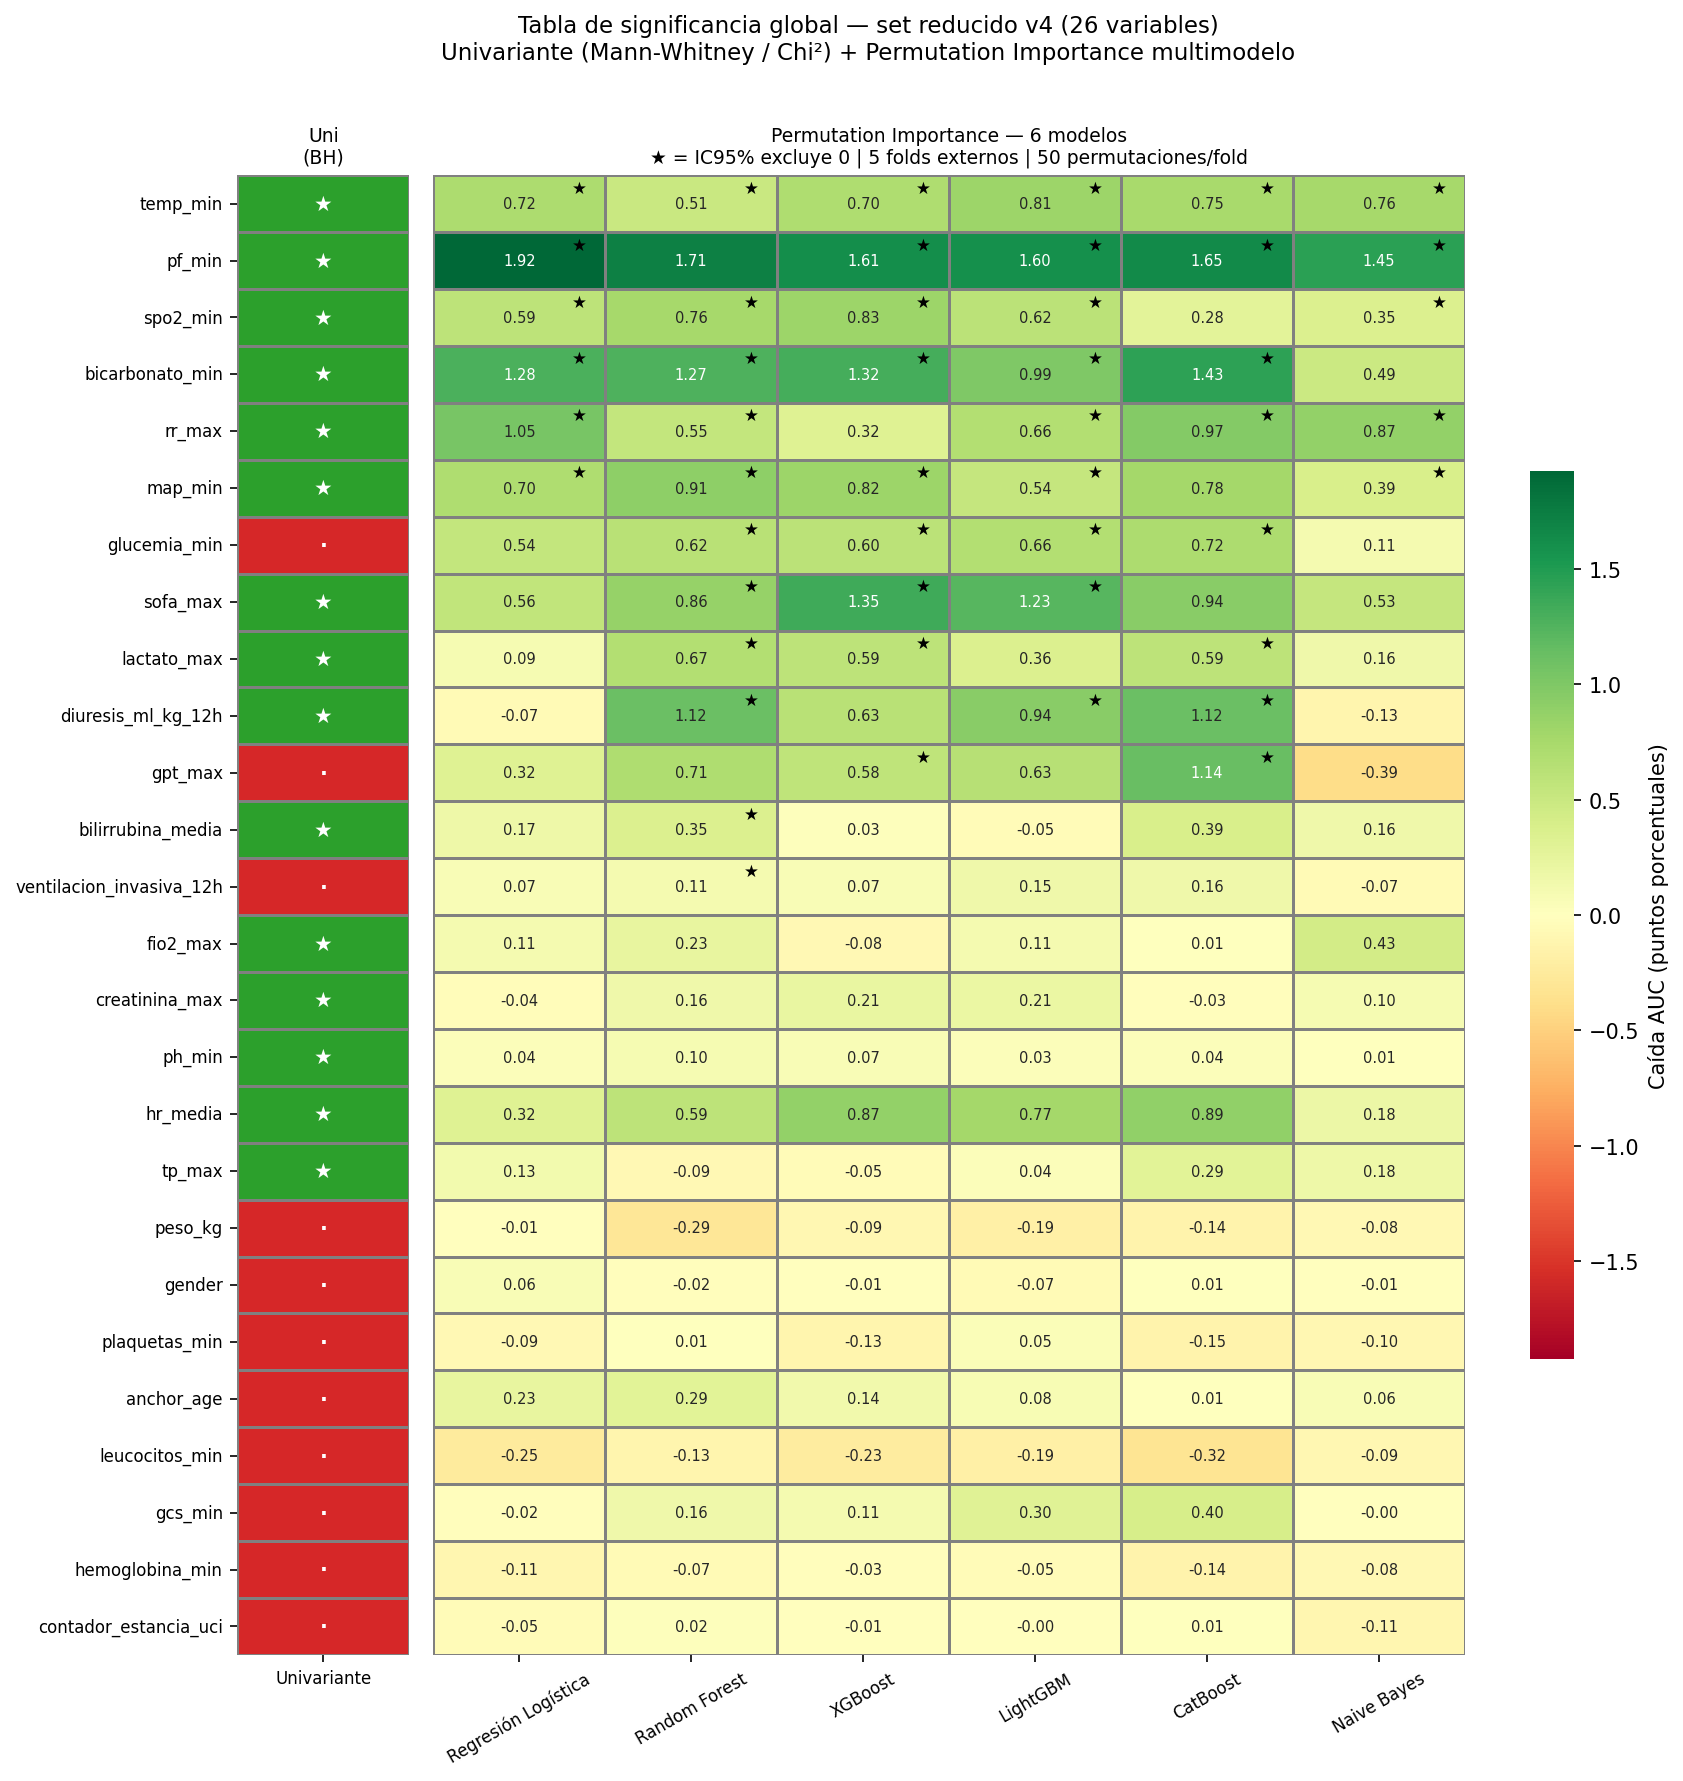
\includegraphics[width=\linewidth]{img/significancia_global_v4l.png}
    \caption{Larga}
  \end{subfigure}
  \caption{Importancia por permutación (caída de AUC al permutar cada variable,
  con IC95\,\%) en las tres ventanas.}
  \label{fig:permutation}
\end{figure}
 
\subsubsection*{Rendimiento \textit{out-of-fold} de la validación interna (MIMIC-IV)}

Las figuras~\ref{fig:oof-corto}--\ref{fig:oof-largo} muestran, para todos los
modelos de cada ventana, las curvas ROC, precisión-recall y de calibración
calculadas sobre las predicciones \textit{out-of-fold} de la validación cruzada
anidada (complemento a la tabla de validación interna).
 
\begin{figure}[htbp]
  \centering
  \begin{subfigure}[t]{0.48\textwidth}\centering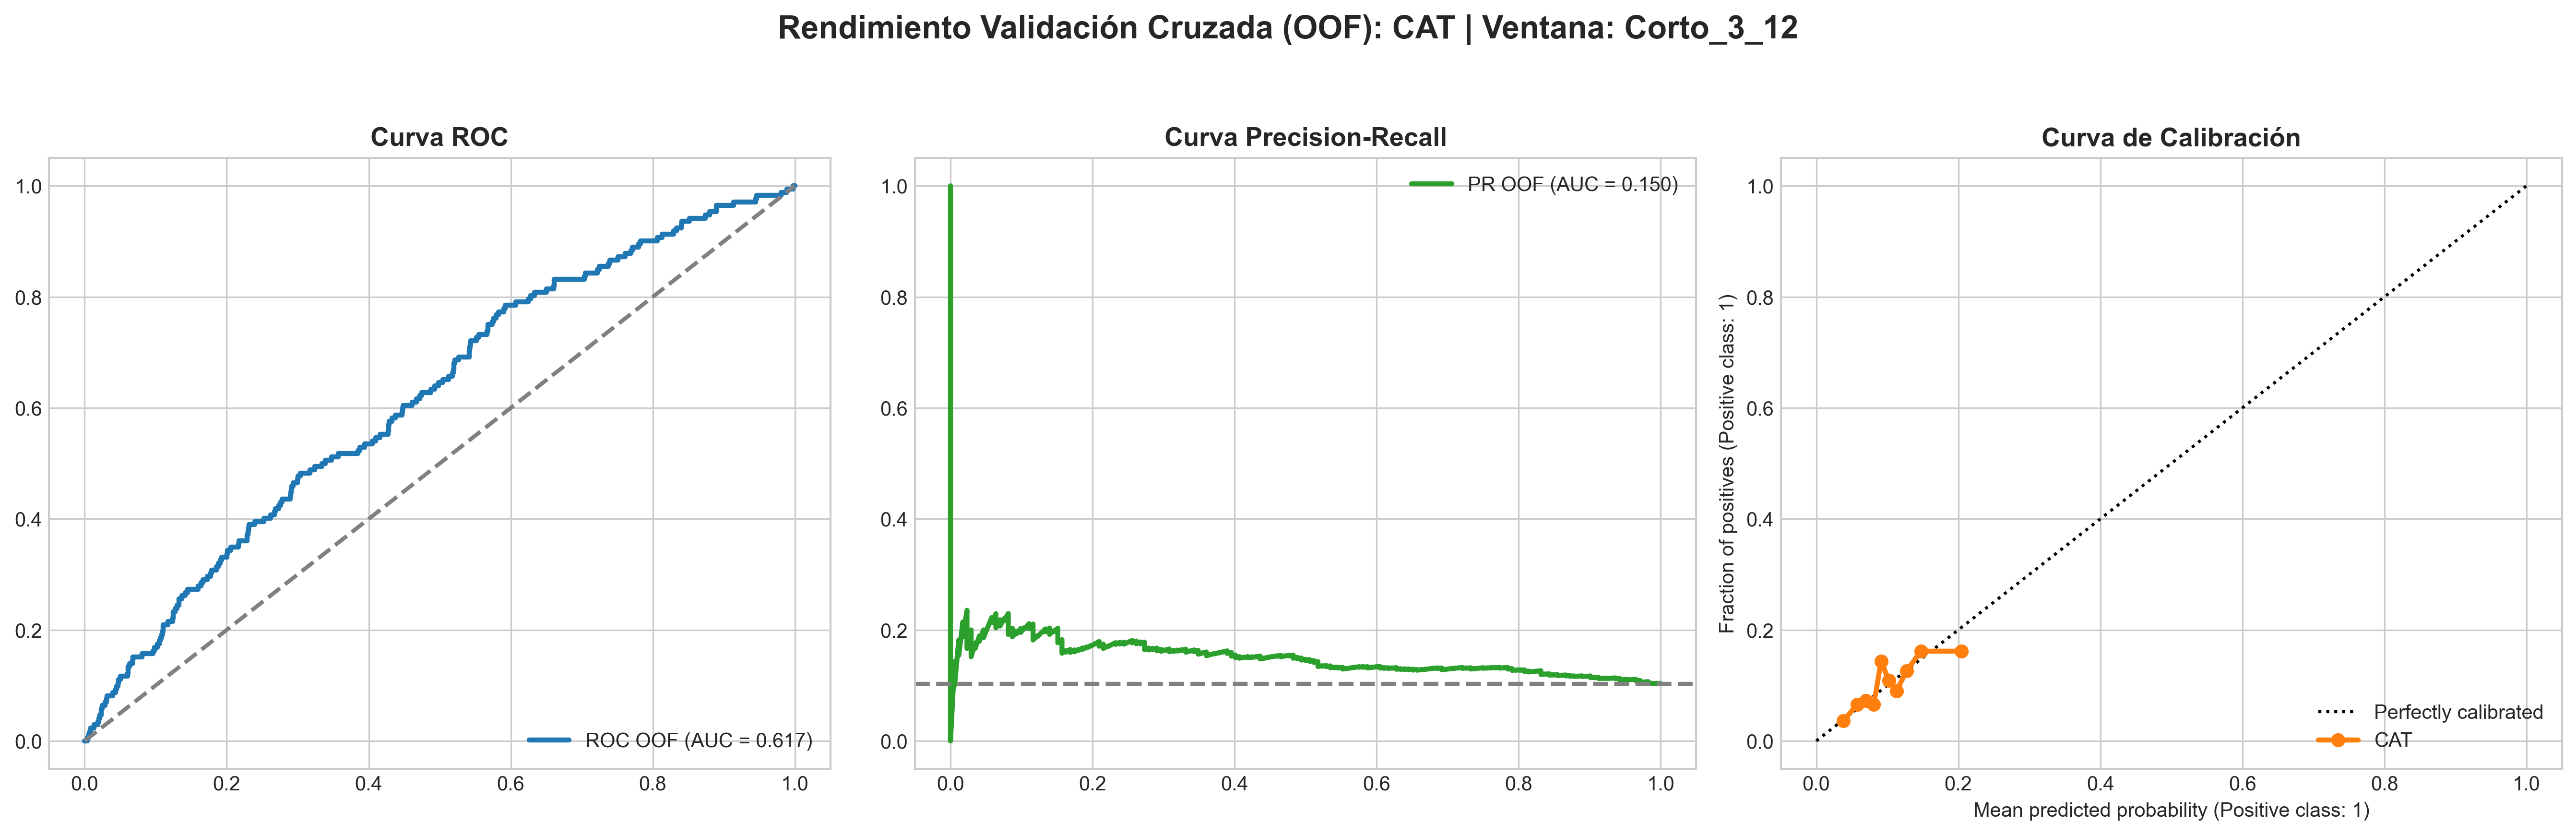
\includegraphics[width=\linewidth]{img/Grafica_OOF_Corto_3_12_CAT.png}\caption{CatBoost}\end{subfigure}\hfill
  \begin{subfigure}[t]{0.48\textwidth}\centering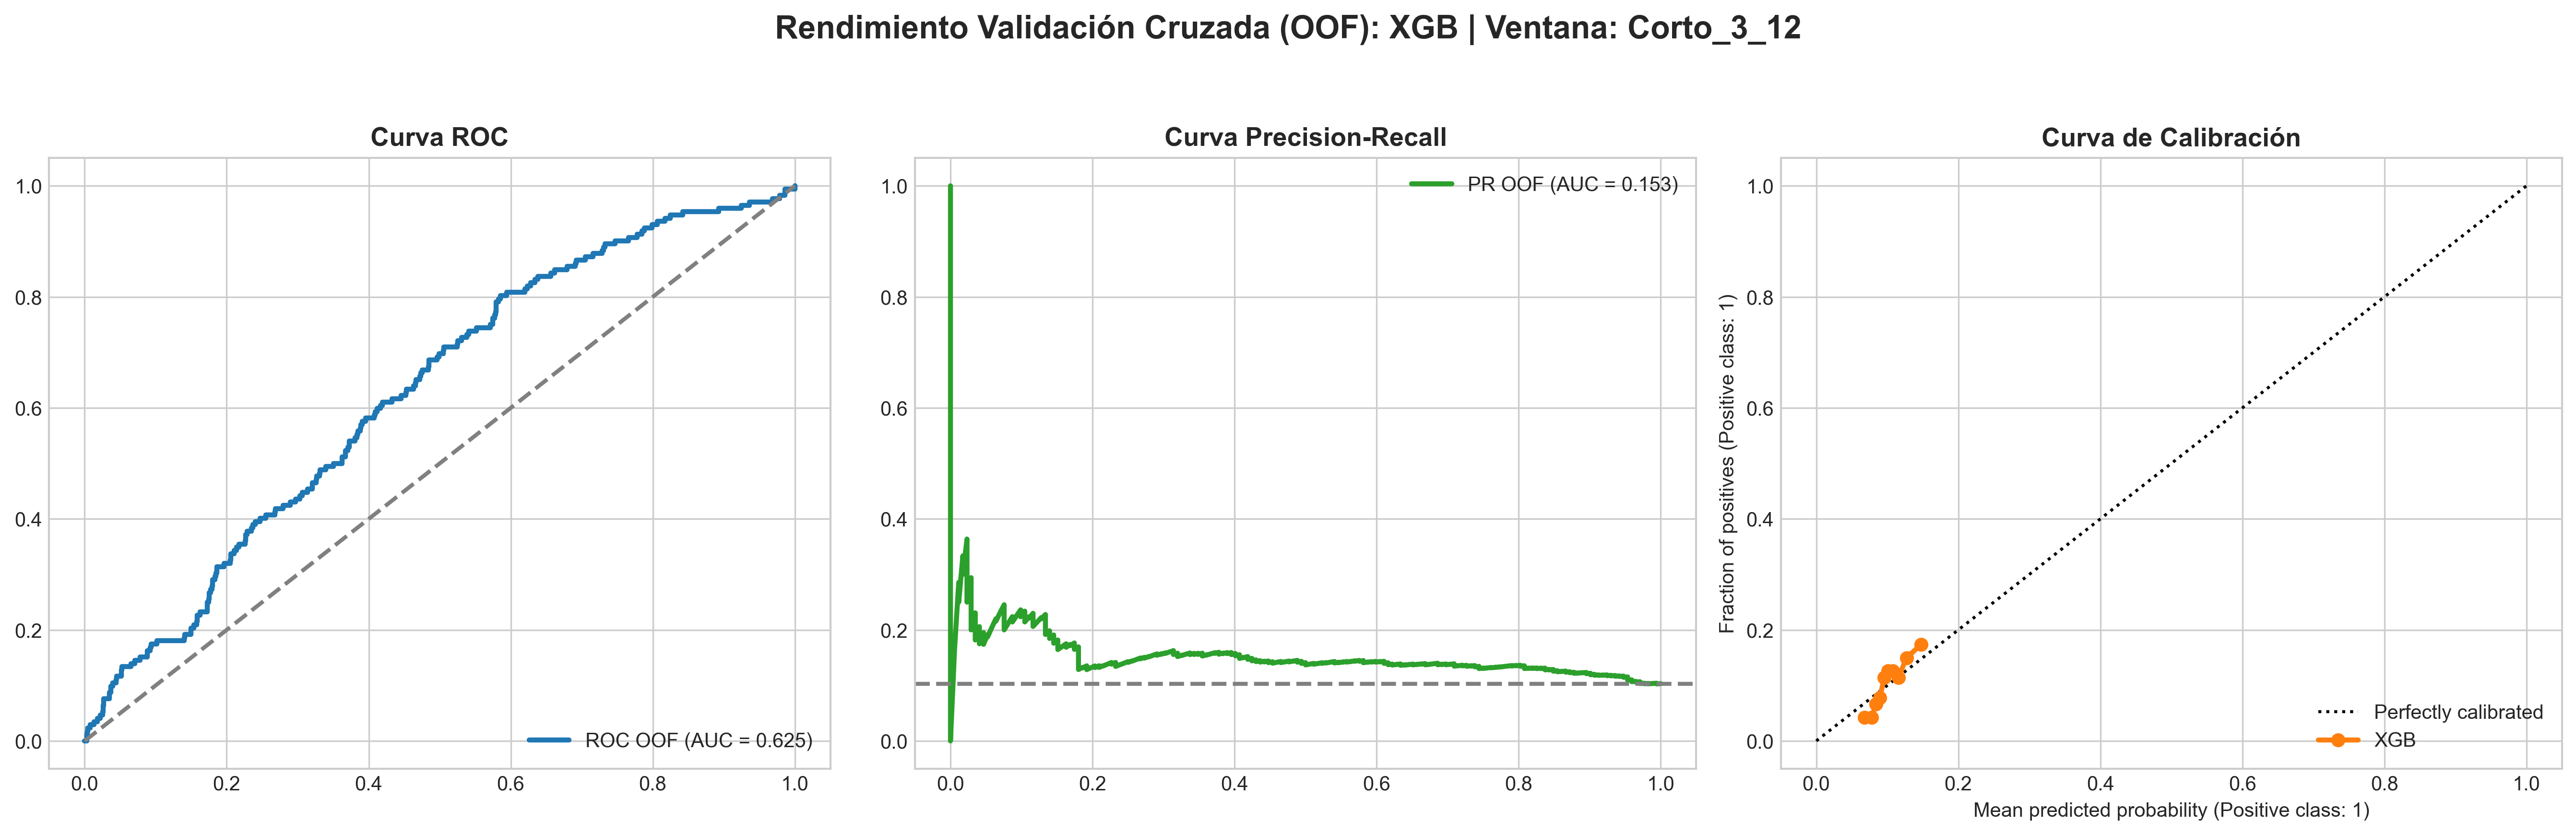
\includegraphics[width=\linewidth]{img/Grafica_OOF_Corto_3_12_XGB.png}\caption{XGBoost}\end{subfigure}\\[6pt]
  \begin{subfigure}[t]{0.48\textwidth}\centering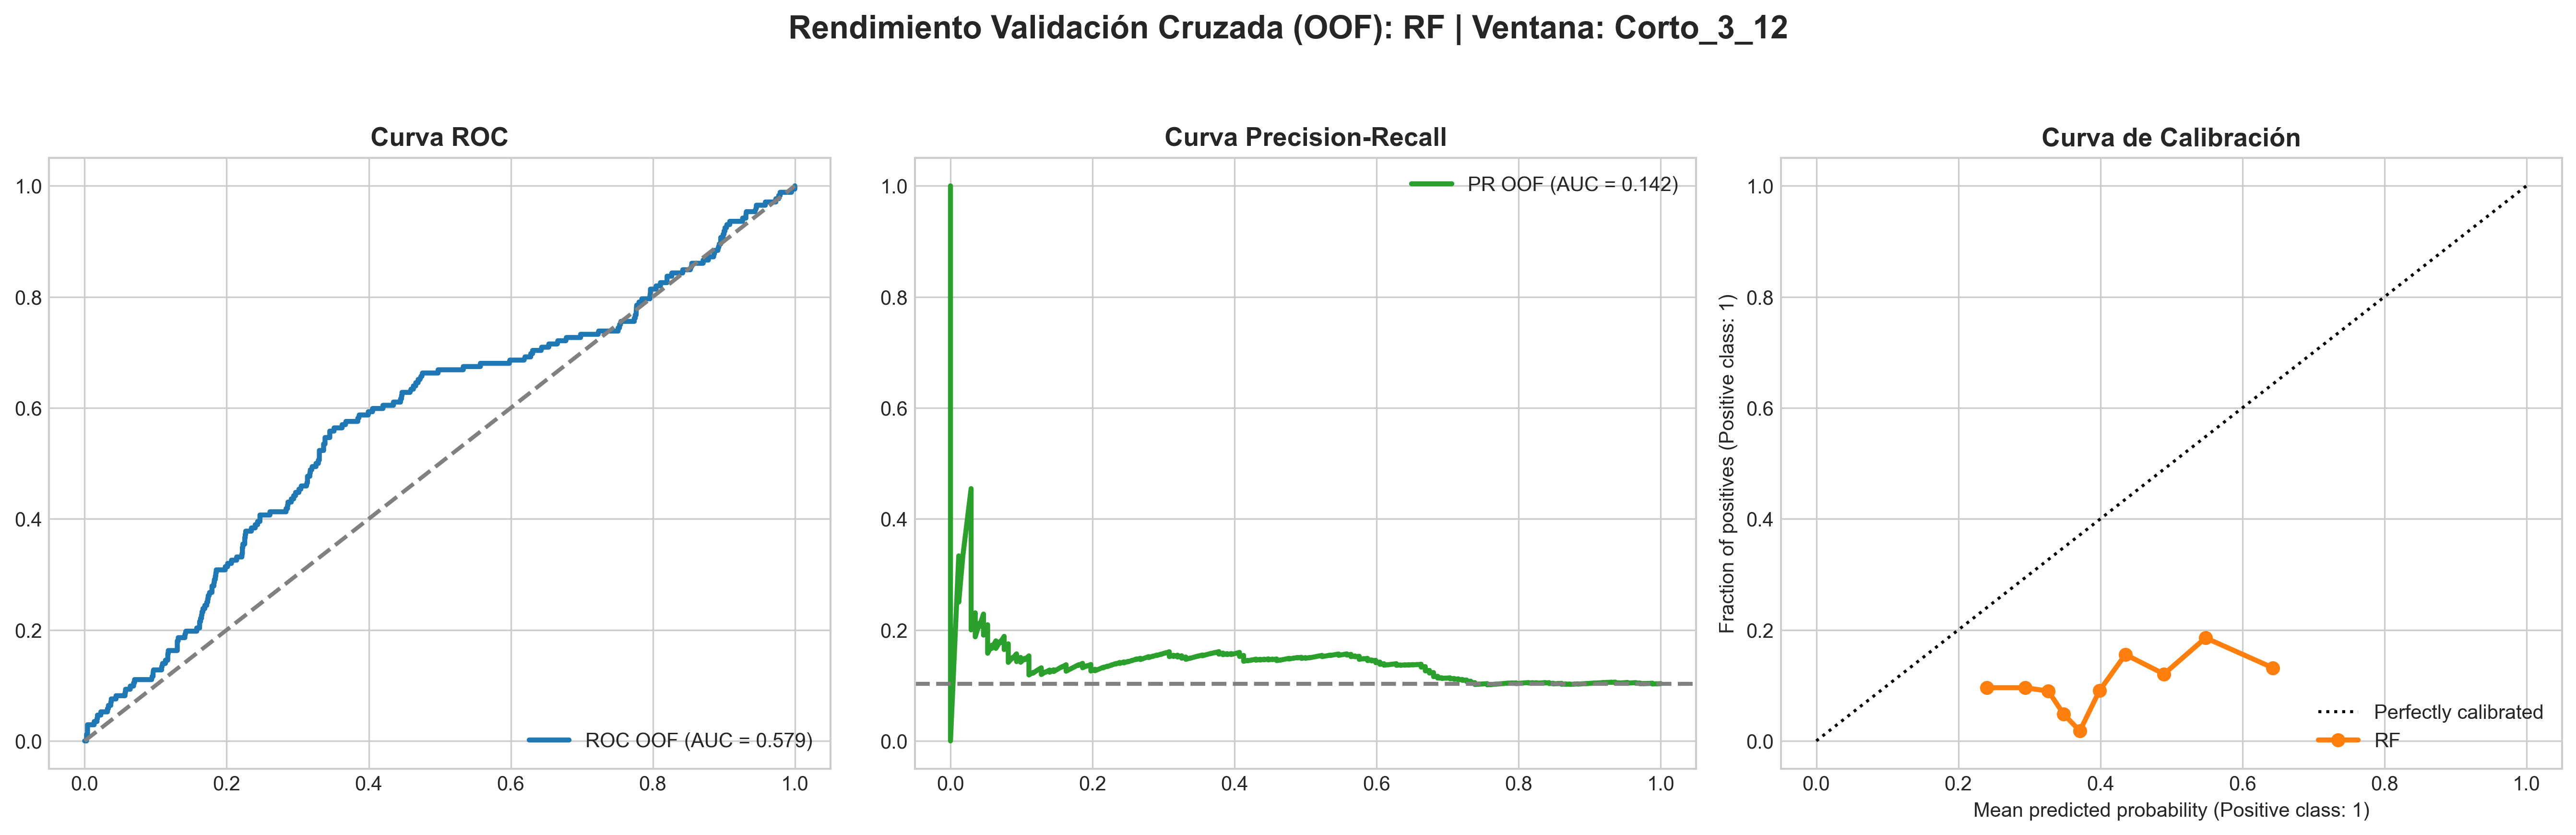
\includegraphics[width=\linewidth]{img/Grafica_OOF_Corto_3_12_RF.png}\caption{Random Forest}\end{subfigure}\hfill
  \begin{subfigure}[t]{0.48\textwidth}\centering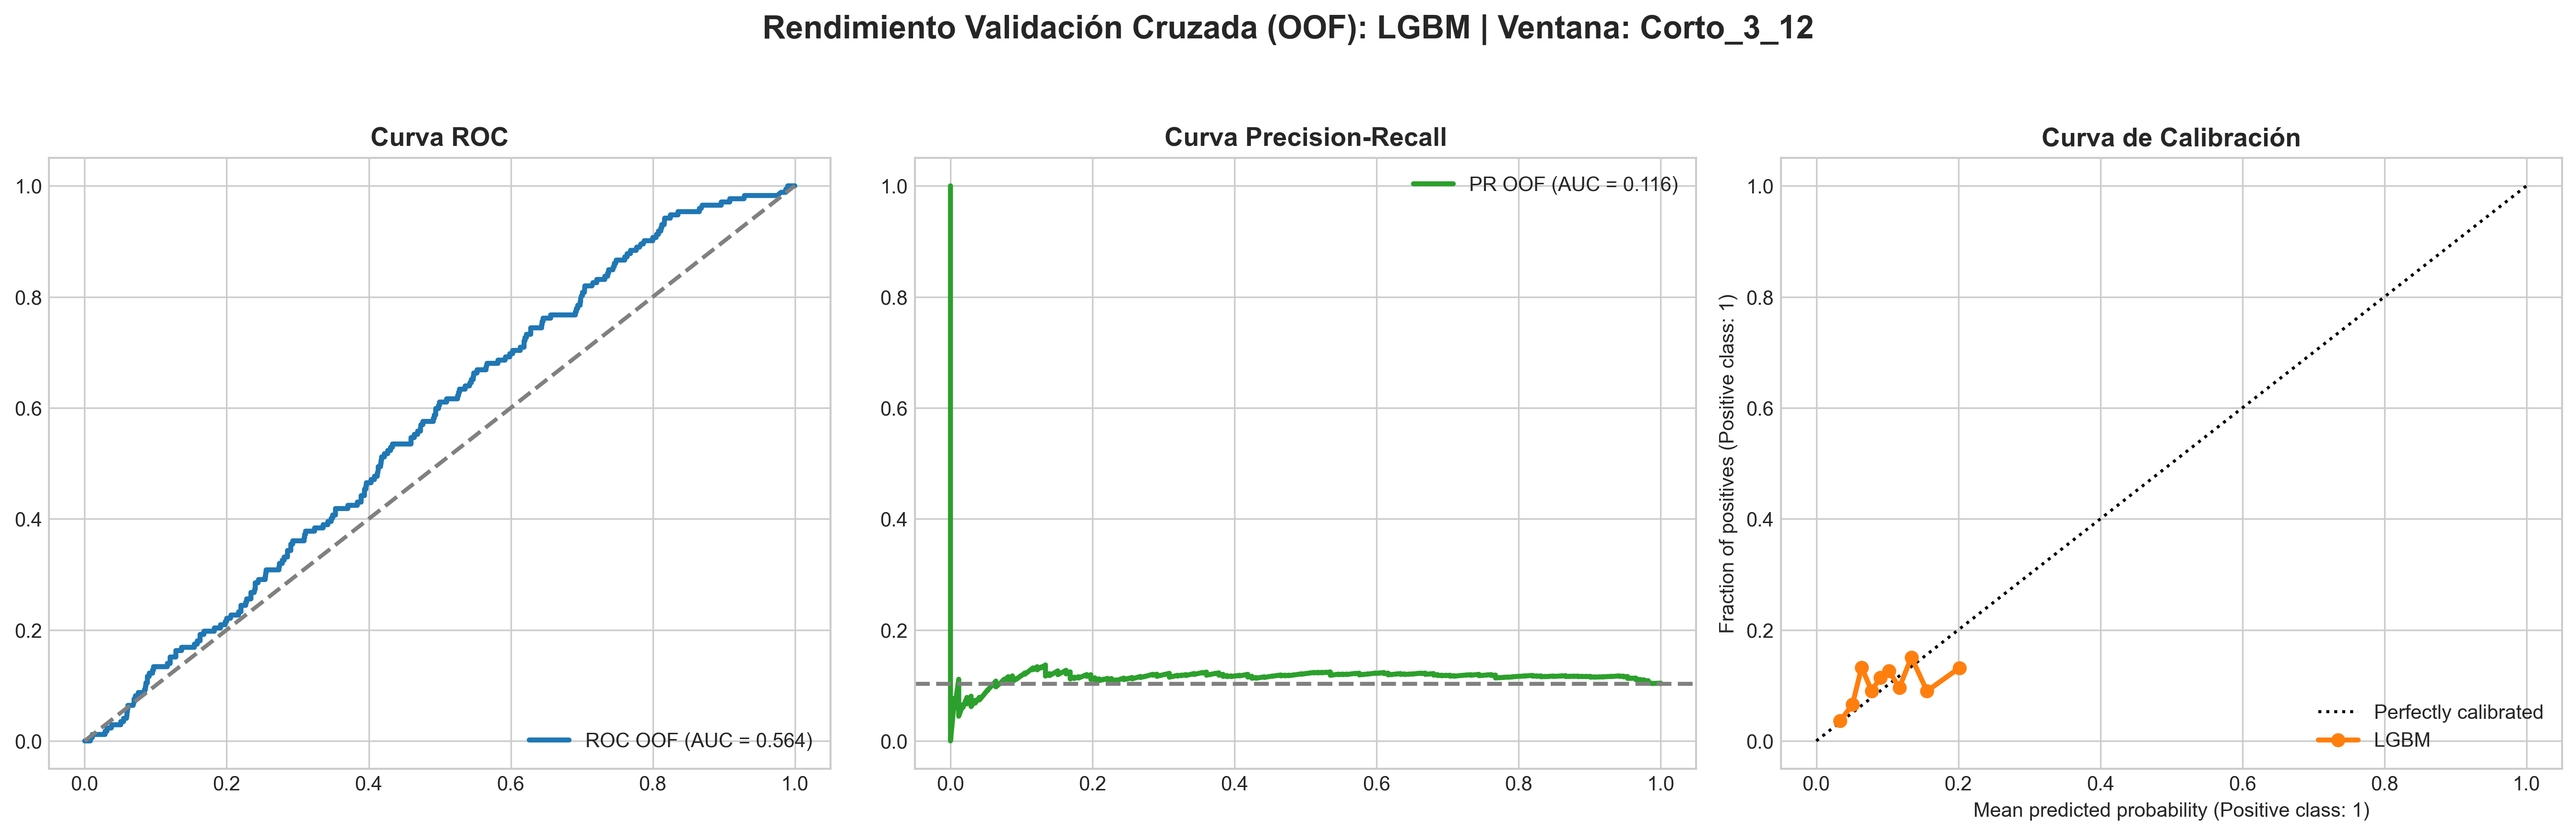
\includegraphics[width=\linewidth]{img/Grafica_OOF_Corto_3_12_LGBM.png}\caption{LightGBM}\end{subfigure}\\[6pt]
  \begin{subfigure}[t]{0.48\textwidth}\centering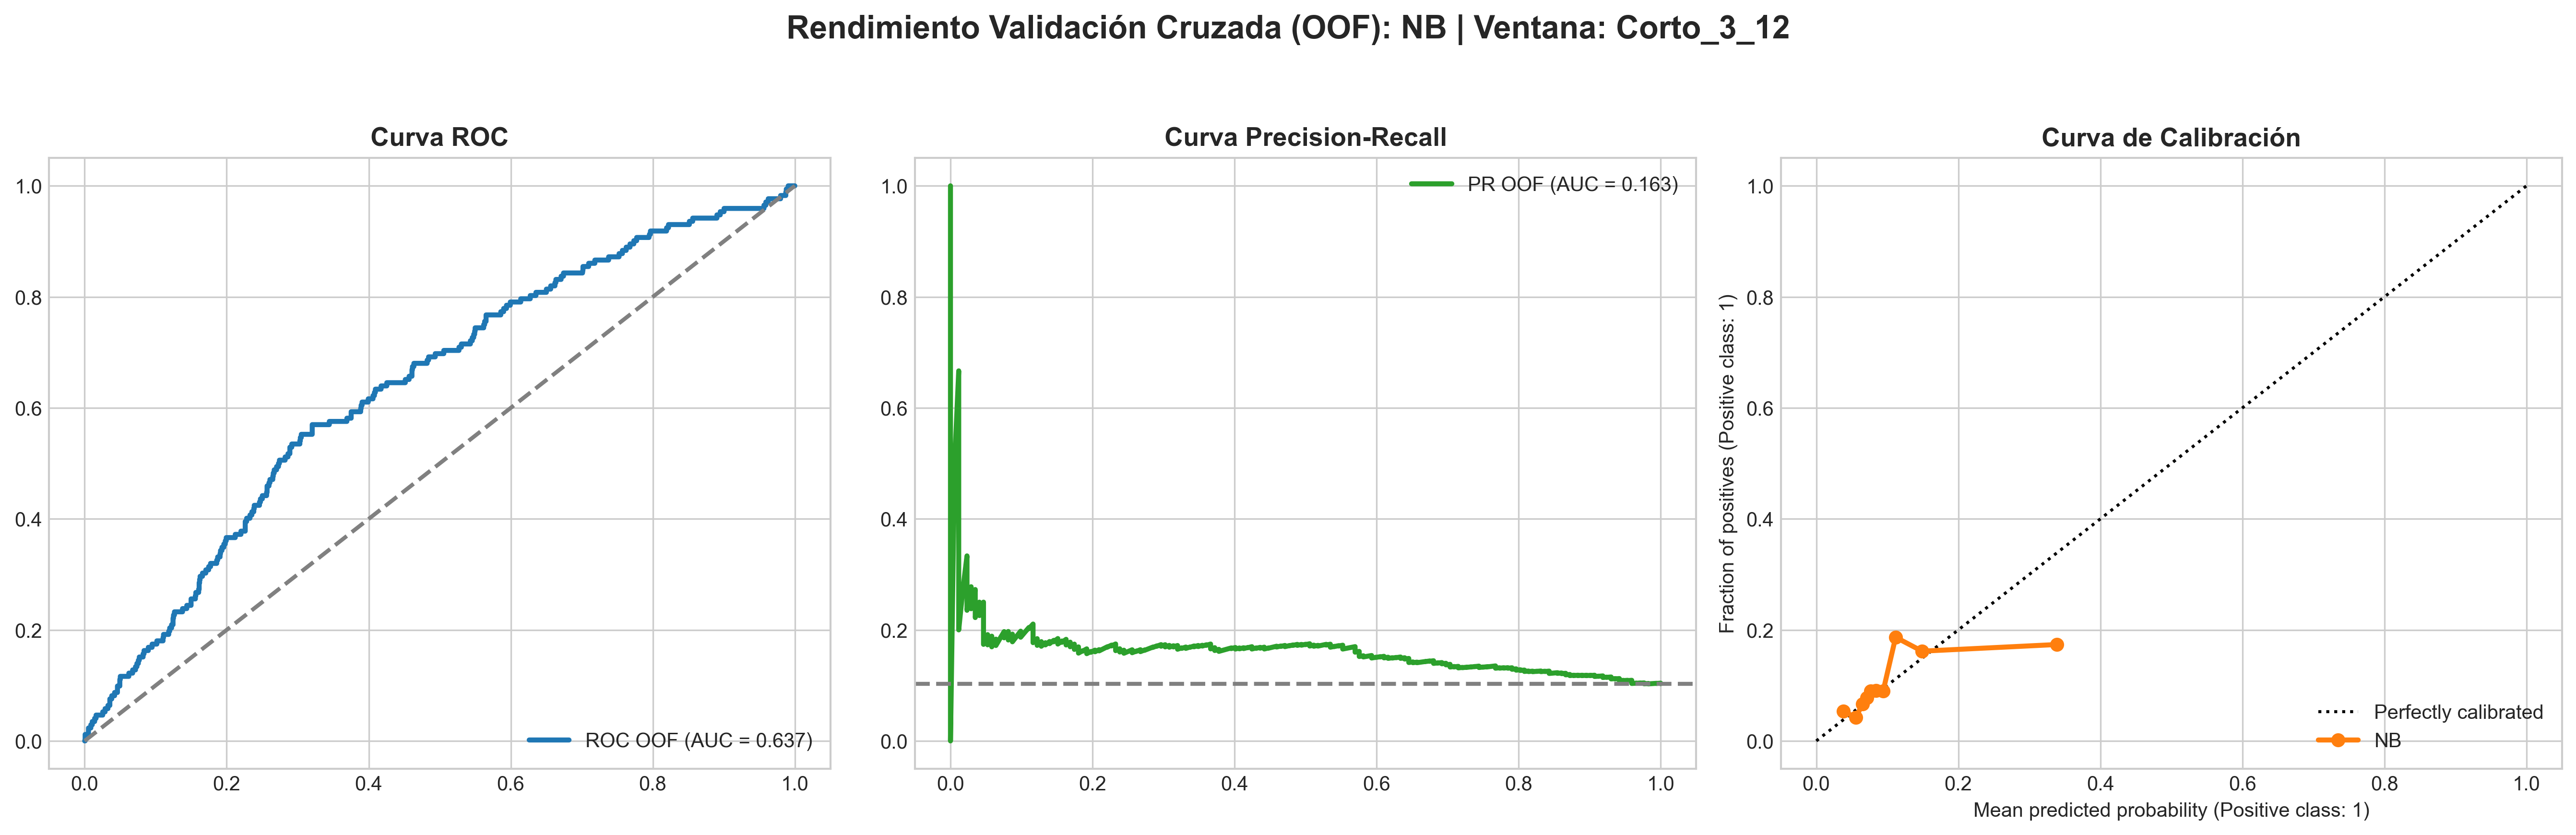
\includegraphics[width=\linewidth]{img/Grafica_OOF_Corto_3_12_NB.png}\caption{Naive Bayes}\end{subfigure}
  \caption{Rendimiento \textit{out-of-fold} de los modelos en la ventana corta (3--12\,h).}
  \label{fig:oof-corto}
\end{figure}
 
\begin{figure}[htbp]
  \centering
  \begin{subfigure}[t]{0.48\textwidth}\centering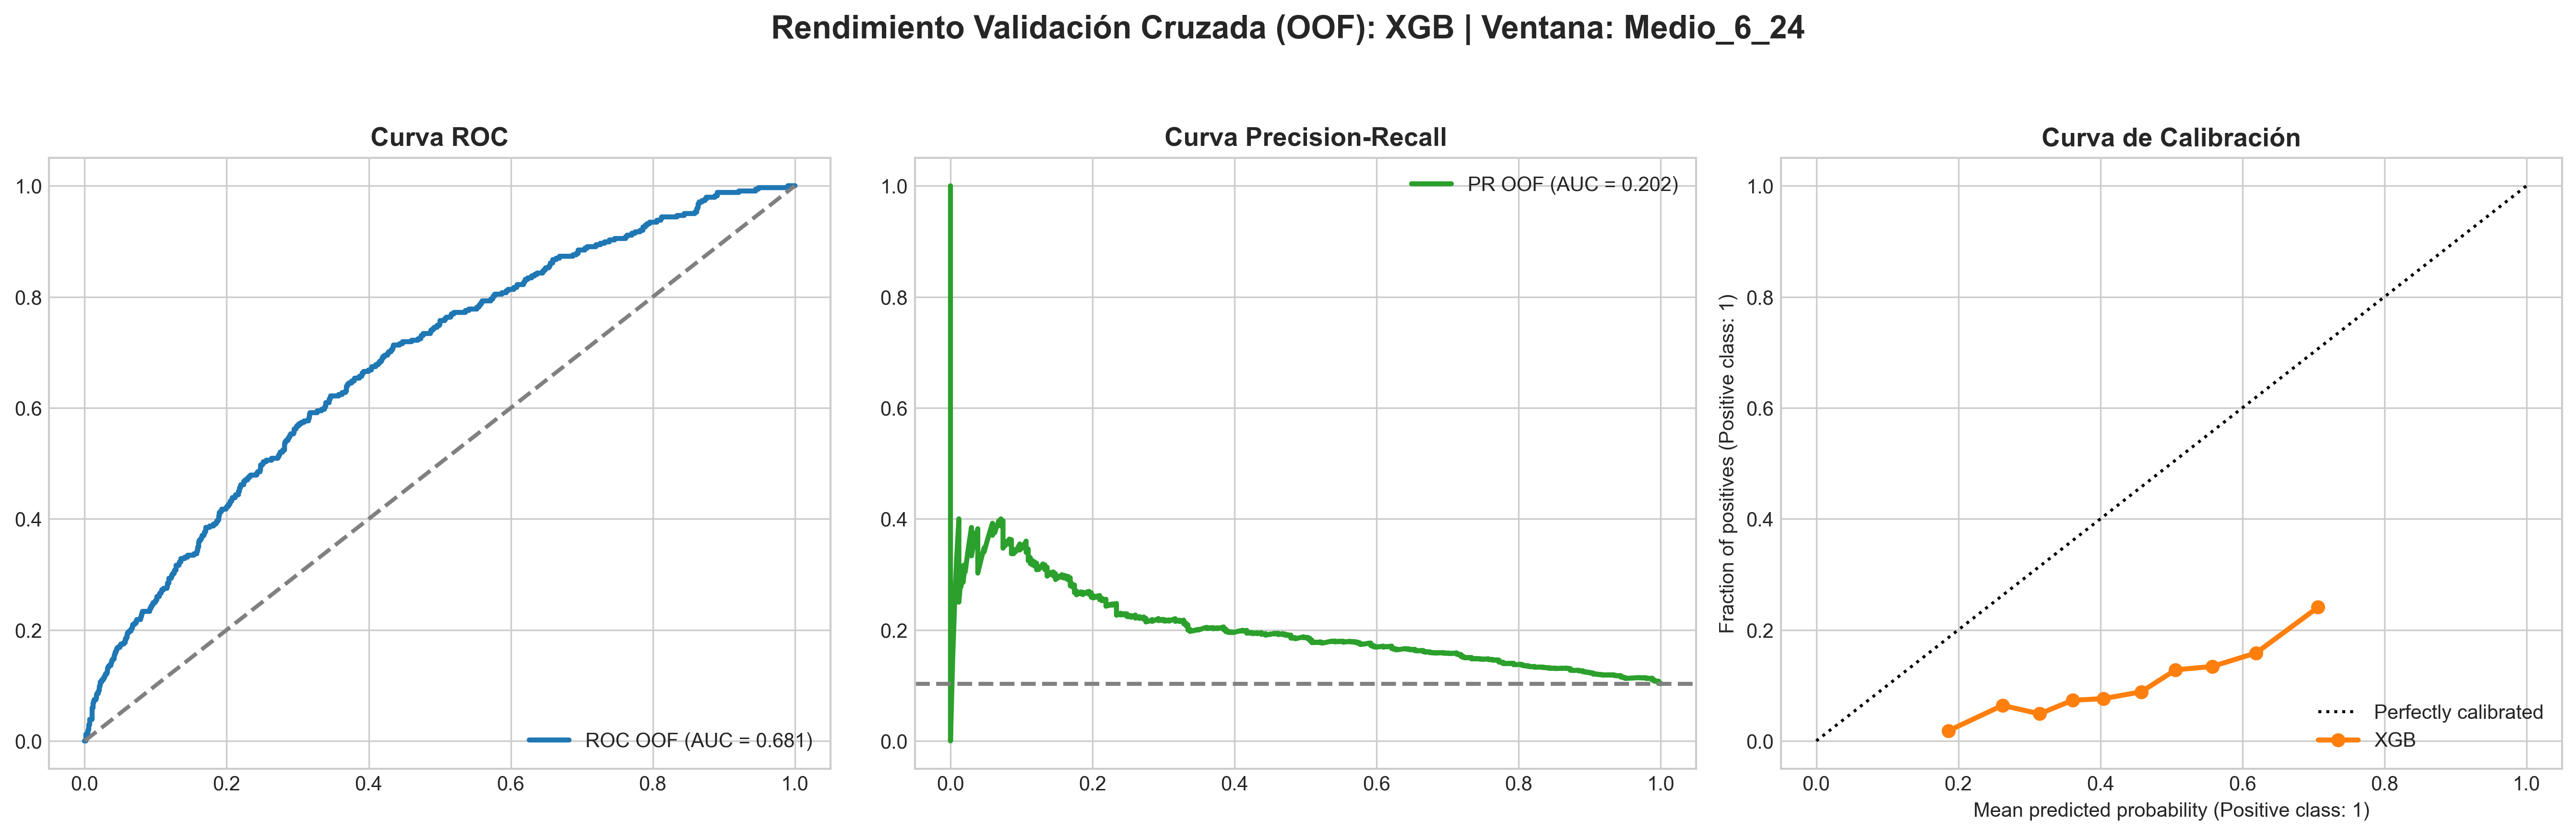
\includegraphics[width=\linewidth]{img/Grafica_OOF_Medio_6_24_XGB.png}\caption{XGBoost}\end{subfigure}\hfill
  \begin{subfigure}[t]{0.48\textwidth}\centering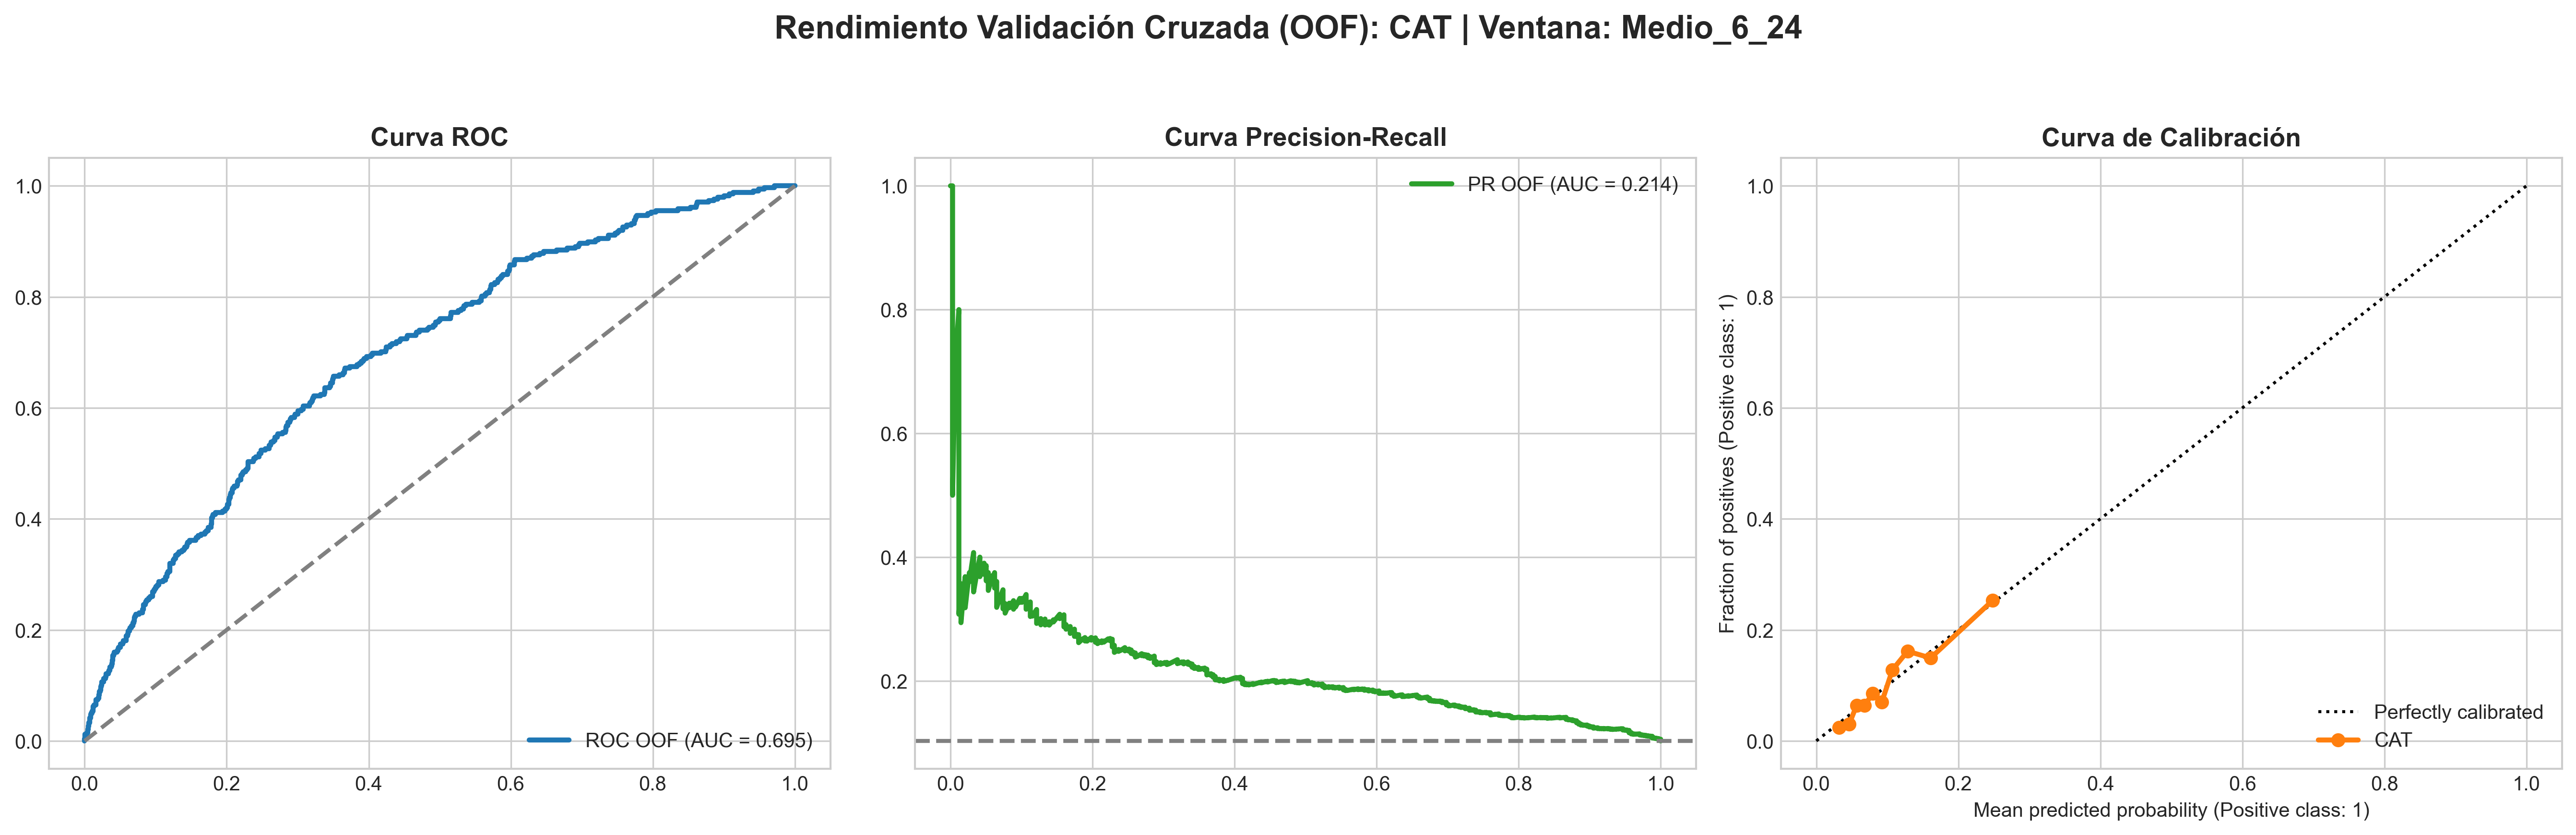
\includegraphics[width=\linewidth]{img/Grafica_OOF_Medio_6_24_CAT.png}\caption{CatBoost}\end{subfigure}\\[6pt]
  \begin{subfigure}[t]{0.48\textwidth}\centering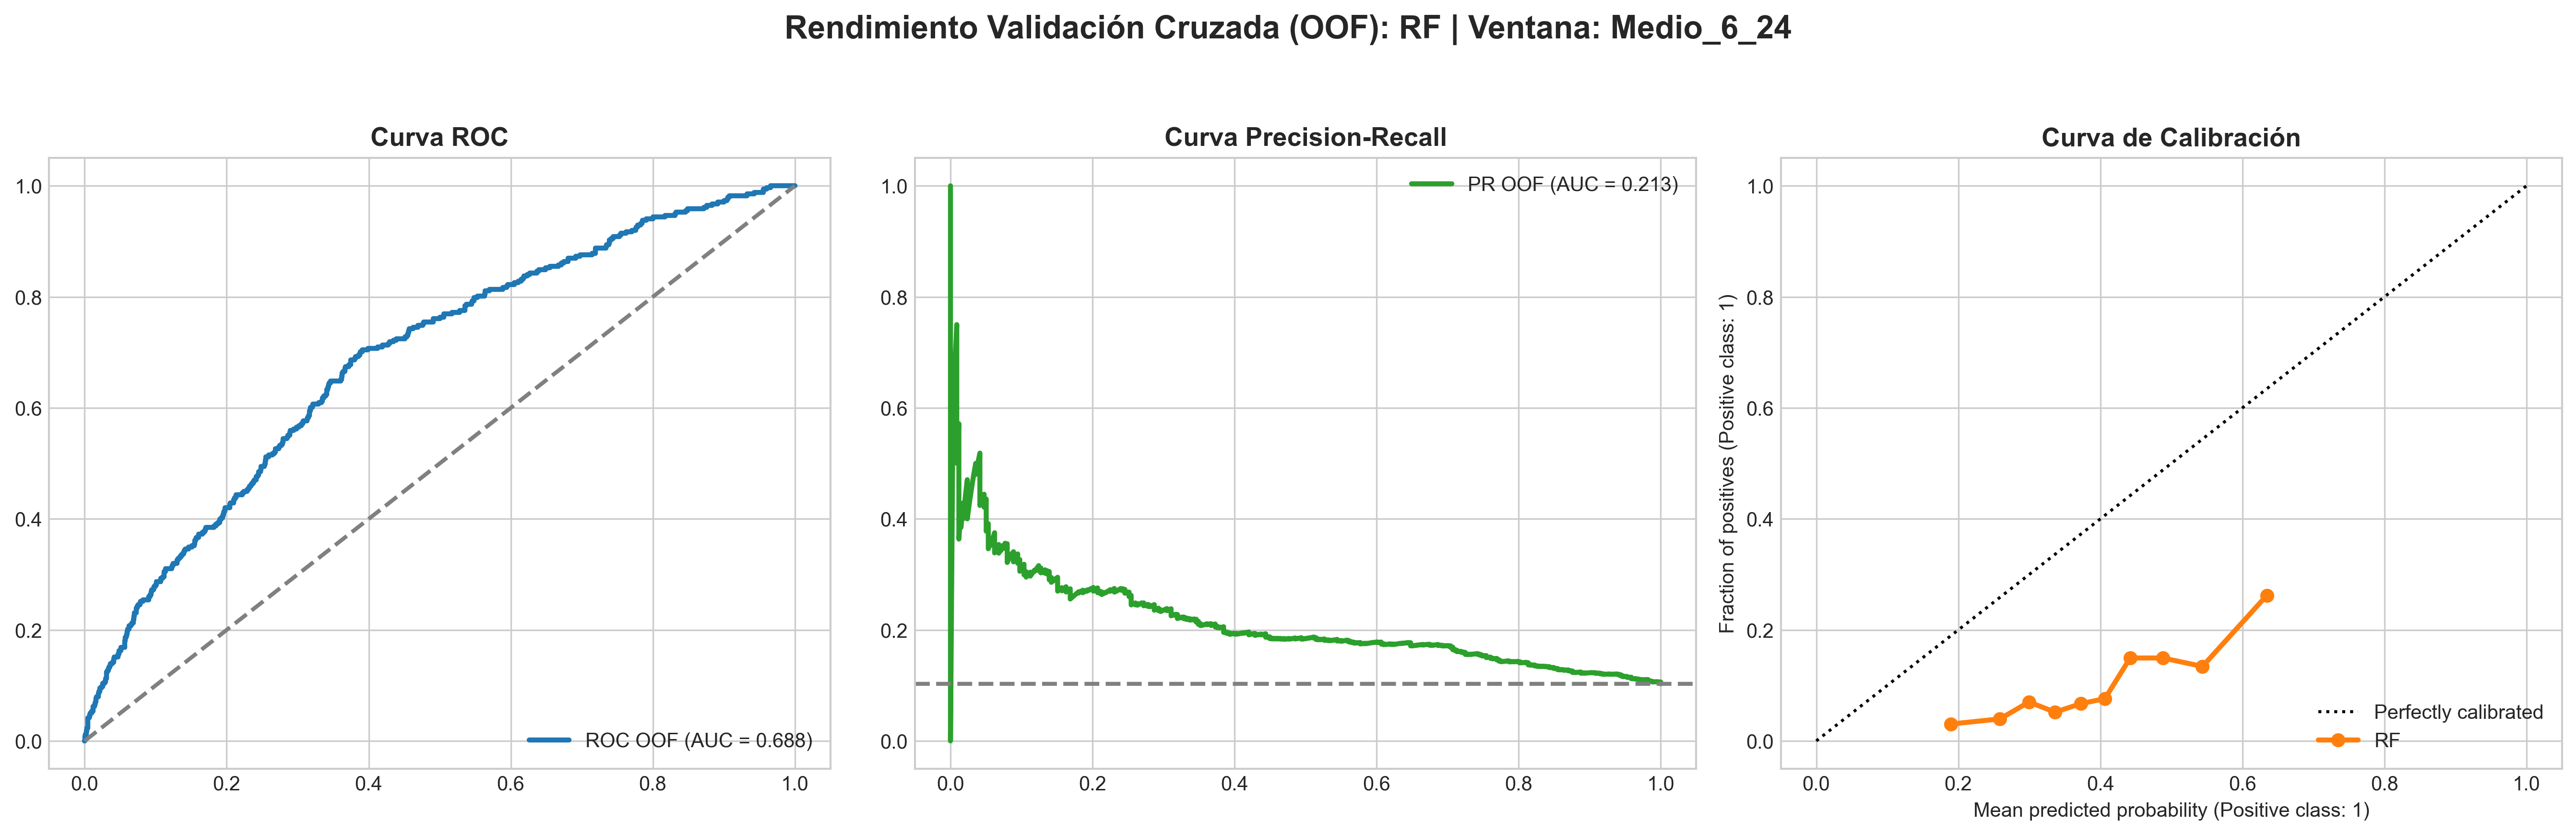
\includegraphics[width=\linewidth]{img/Grafica_OOF_Medio_6_24_RF.png}\caption{Random Forest}\end{subfigure}\hfill
  \begin{subfigure}[t]{0.48\textwidth}\centering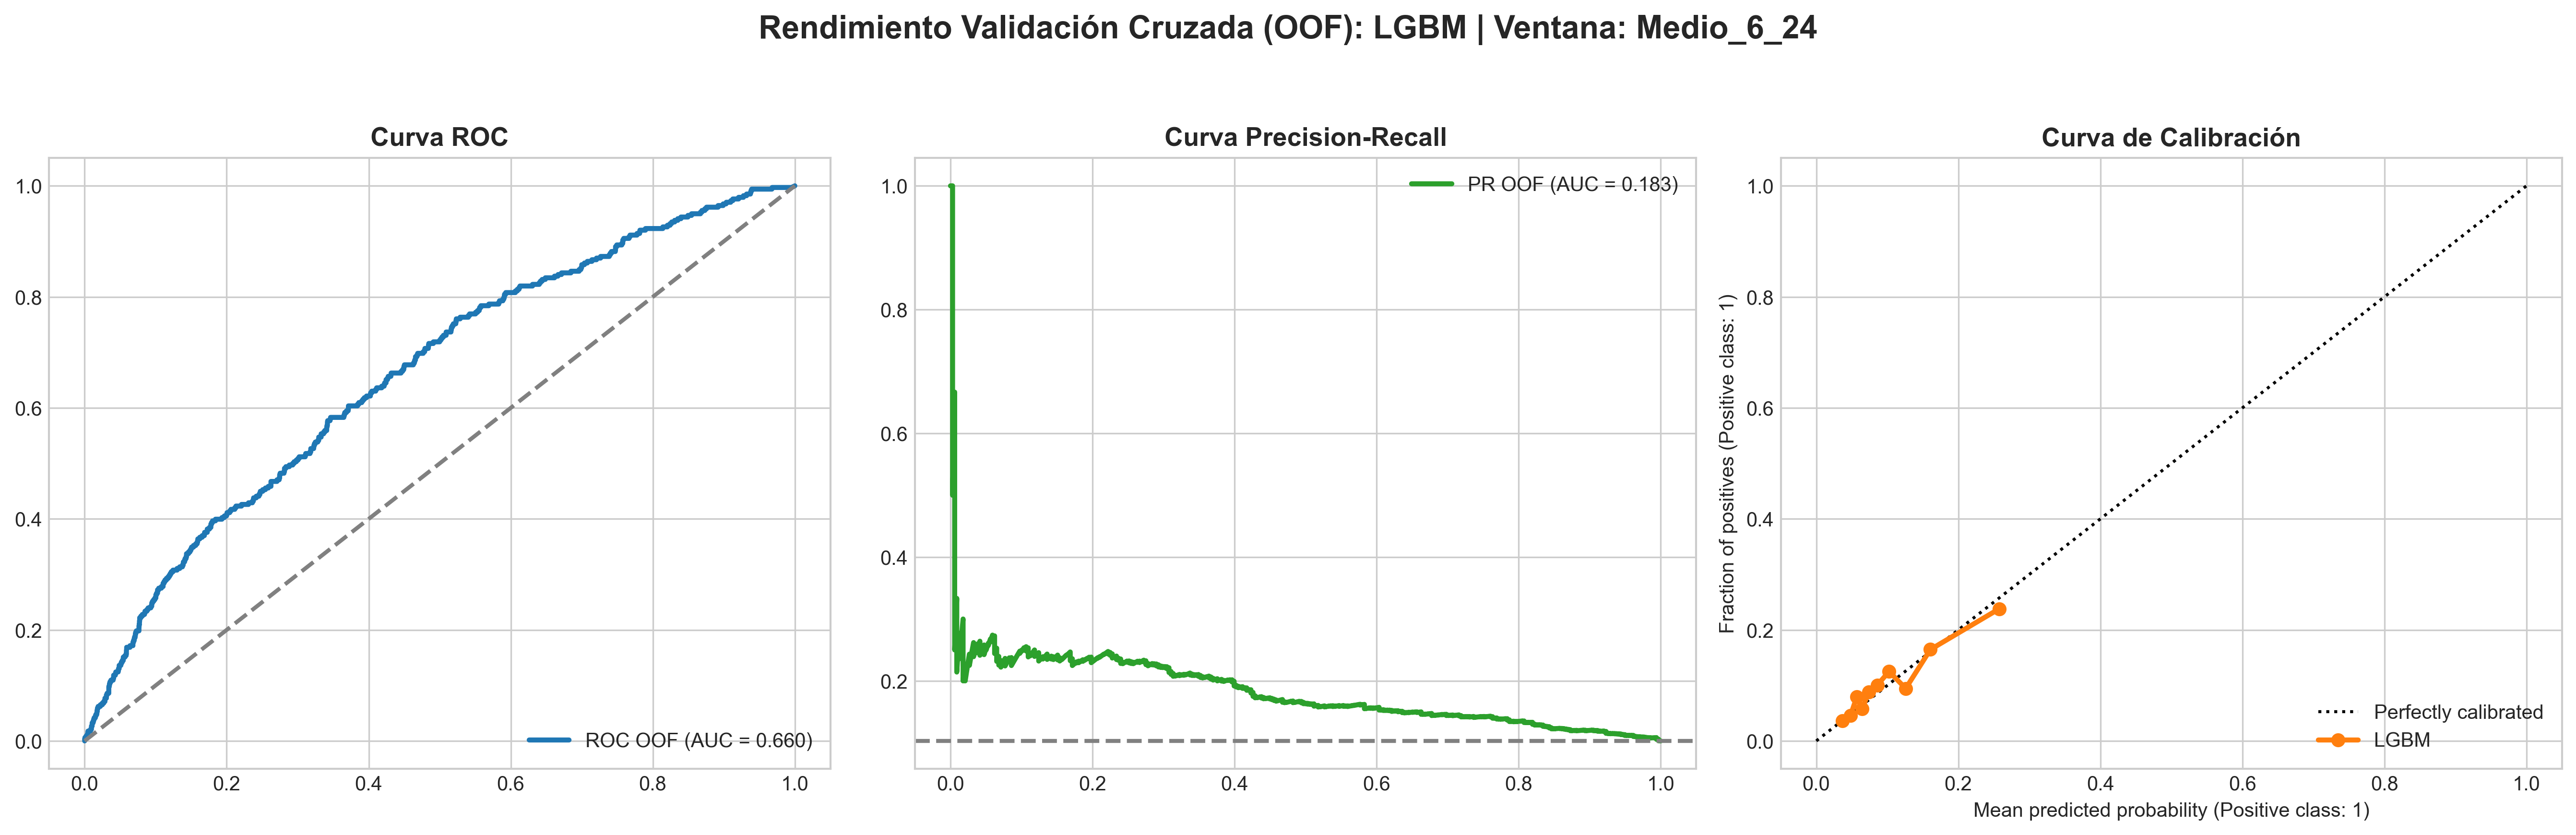
\includegraphics[width=\linewidth]{img/Grafica_OOF_Medio_6_24_LGBM.png}\caption{LightGBM}\end{subfigure}\\[6pt]
  \begin{subfigure}[t]{0.48\textwidth}\centering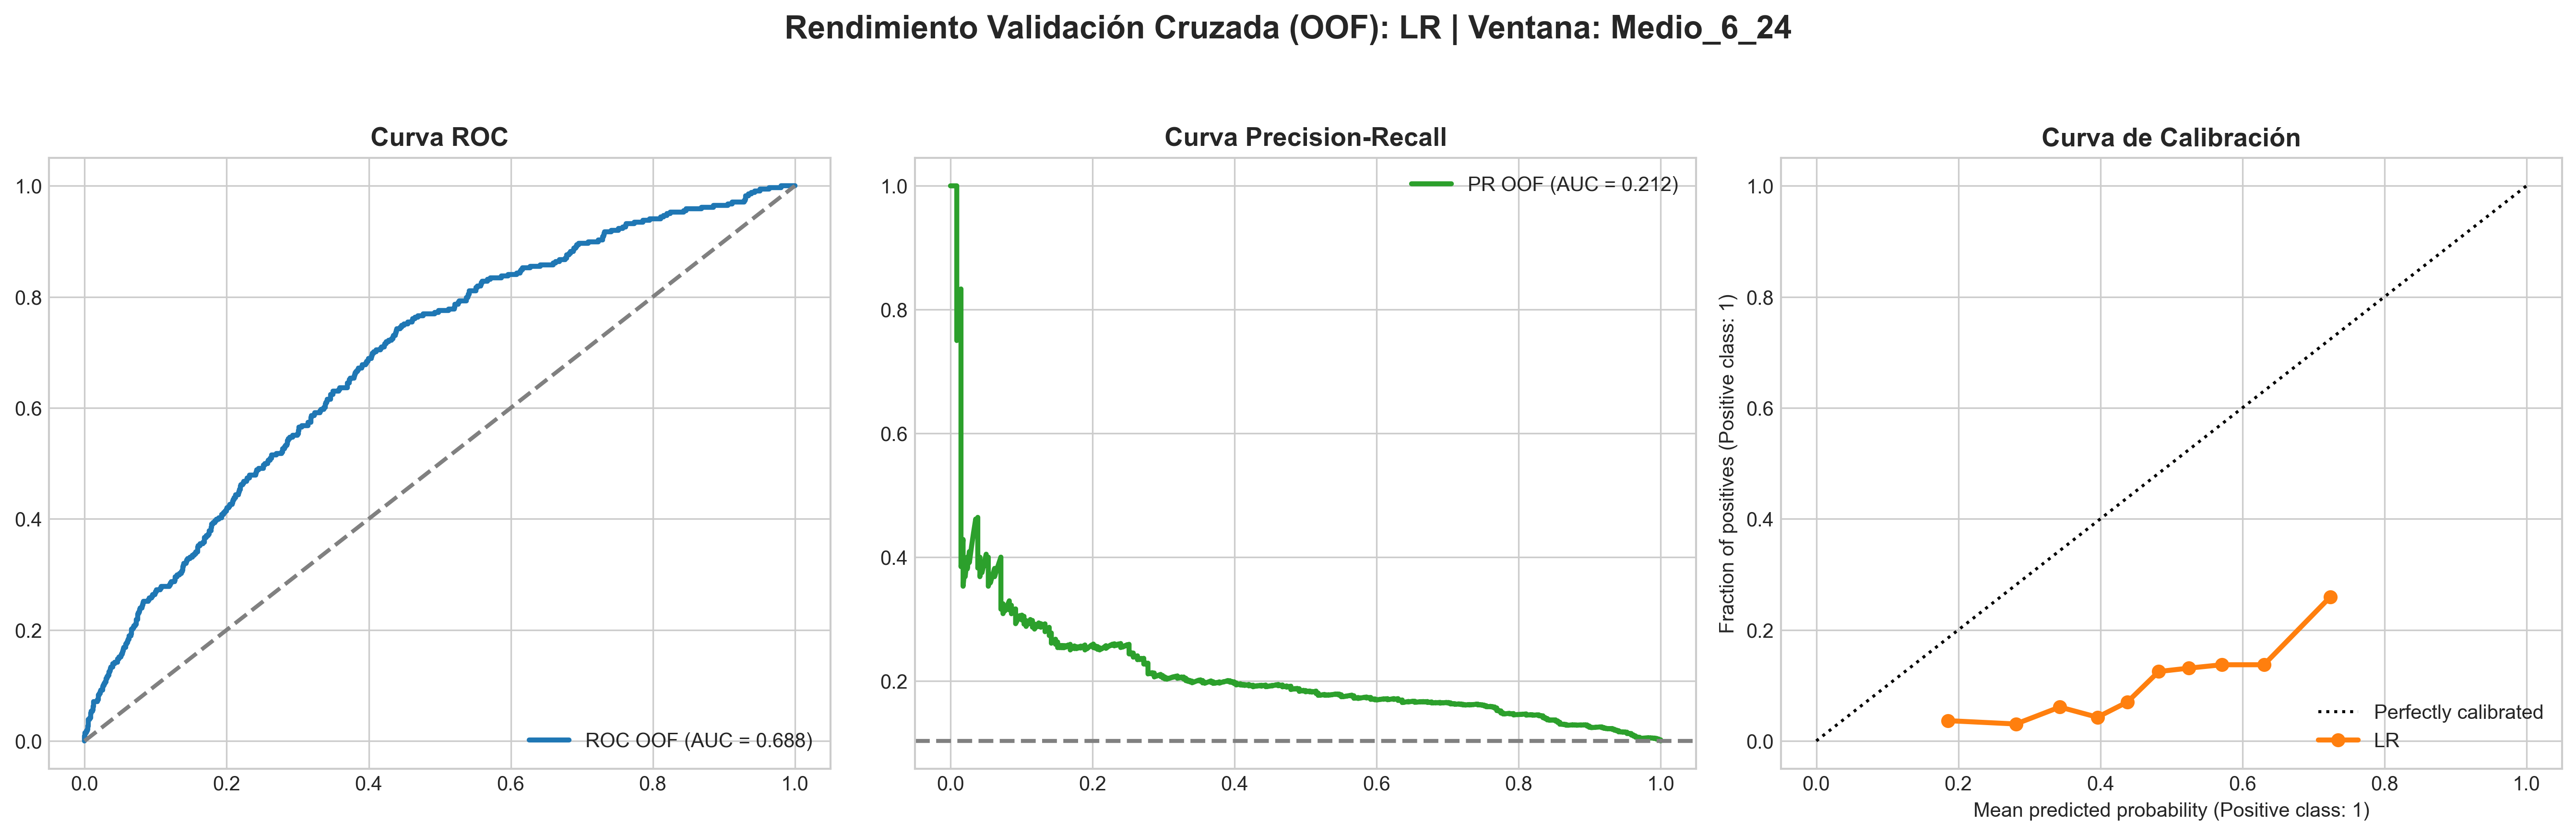
\includegraphics[width=\linewidth]{img/Grafica_OOF_Medio_6_24_LR.png}\caption{Regresión logística}\end{subfigure}\hfill
  \begin{subfigure}[t]{0.48\textwidth}\centering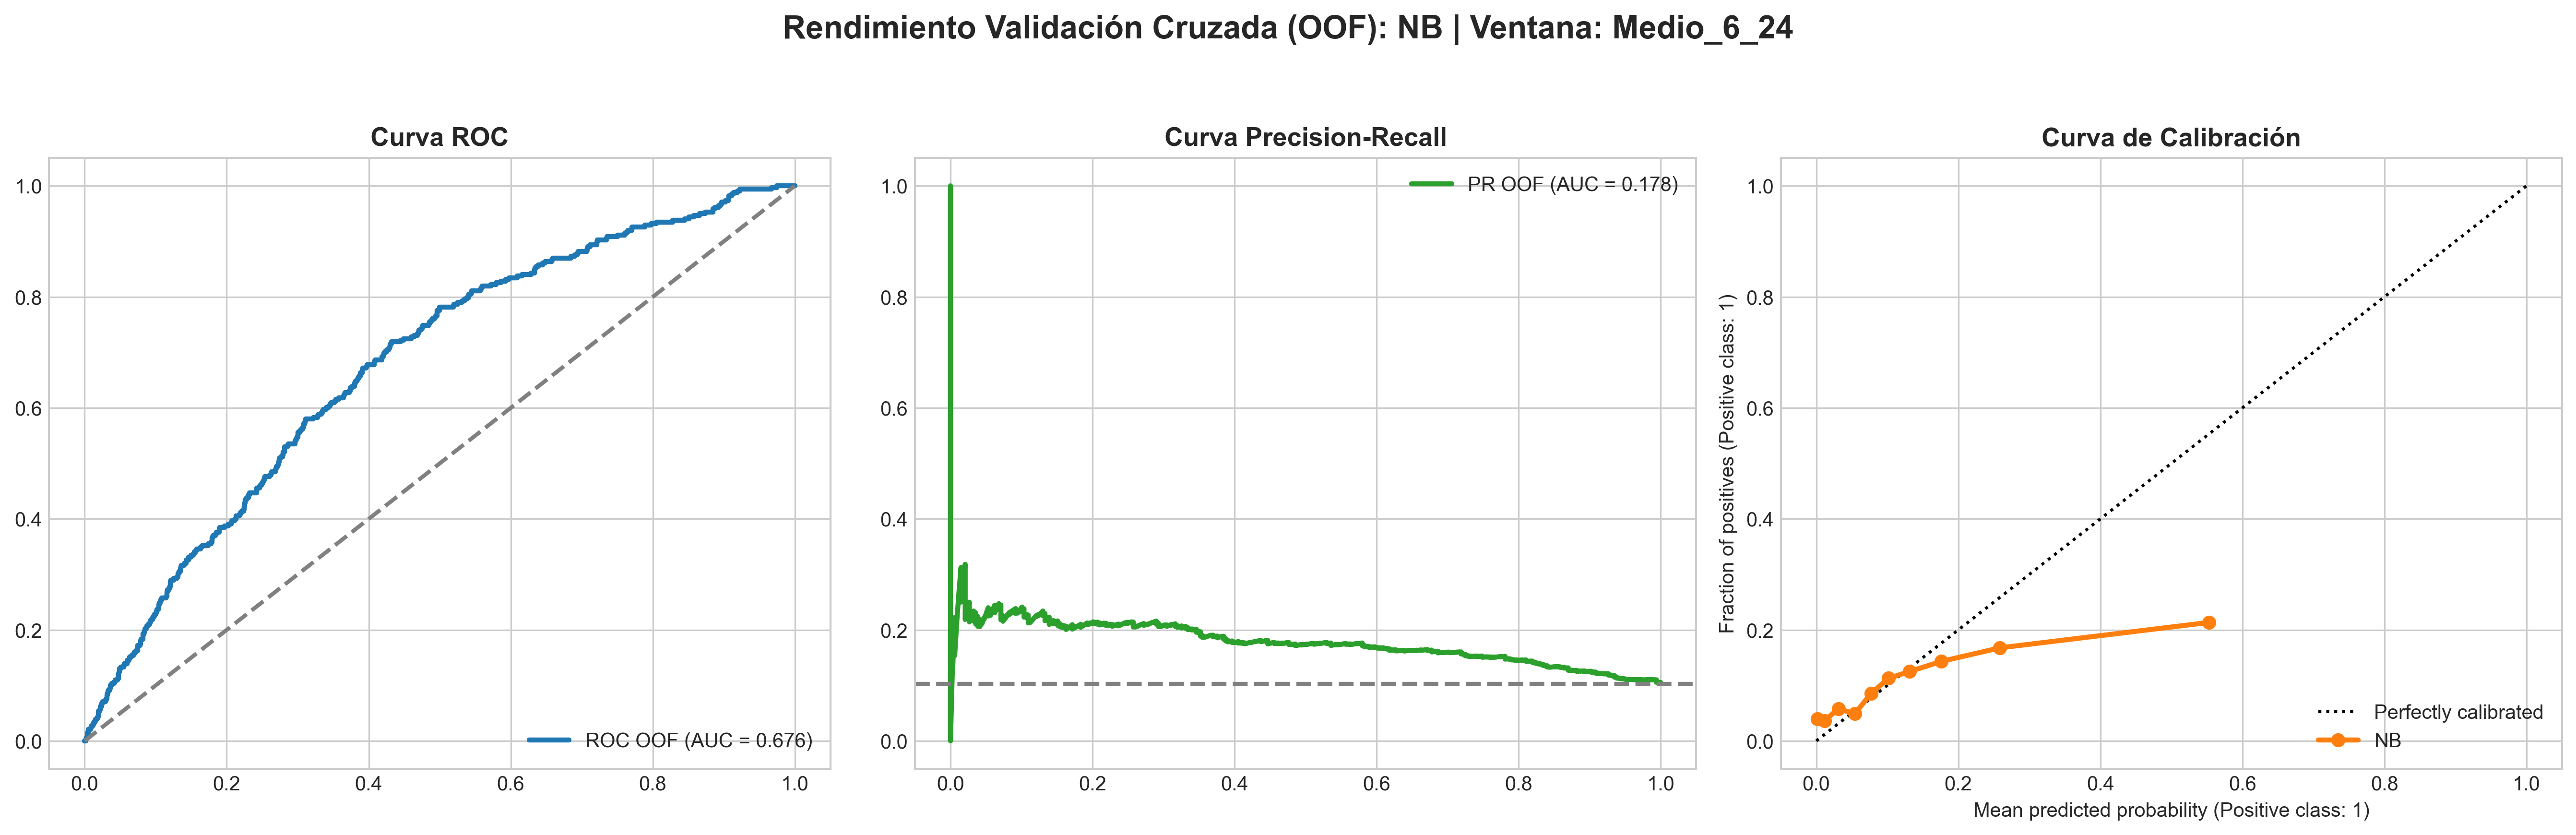
\includegraphics[width=\linewidth]{img/Grafica_OOF_Medio_6_24_NB.png}\caption{Naive Bayes}\end{subfigure}
  \caption{Rendimiento \textit{out-of-fold} de los modelos en la ventana media (6--24\,h).}
  \label{fig:oof-medio}
\end{figure}
 
\begin{figure}[htbp]
  \centering
  \begin{subfigure}[t]{0.48\textwidth}\centering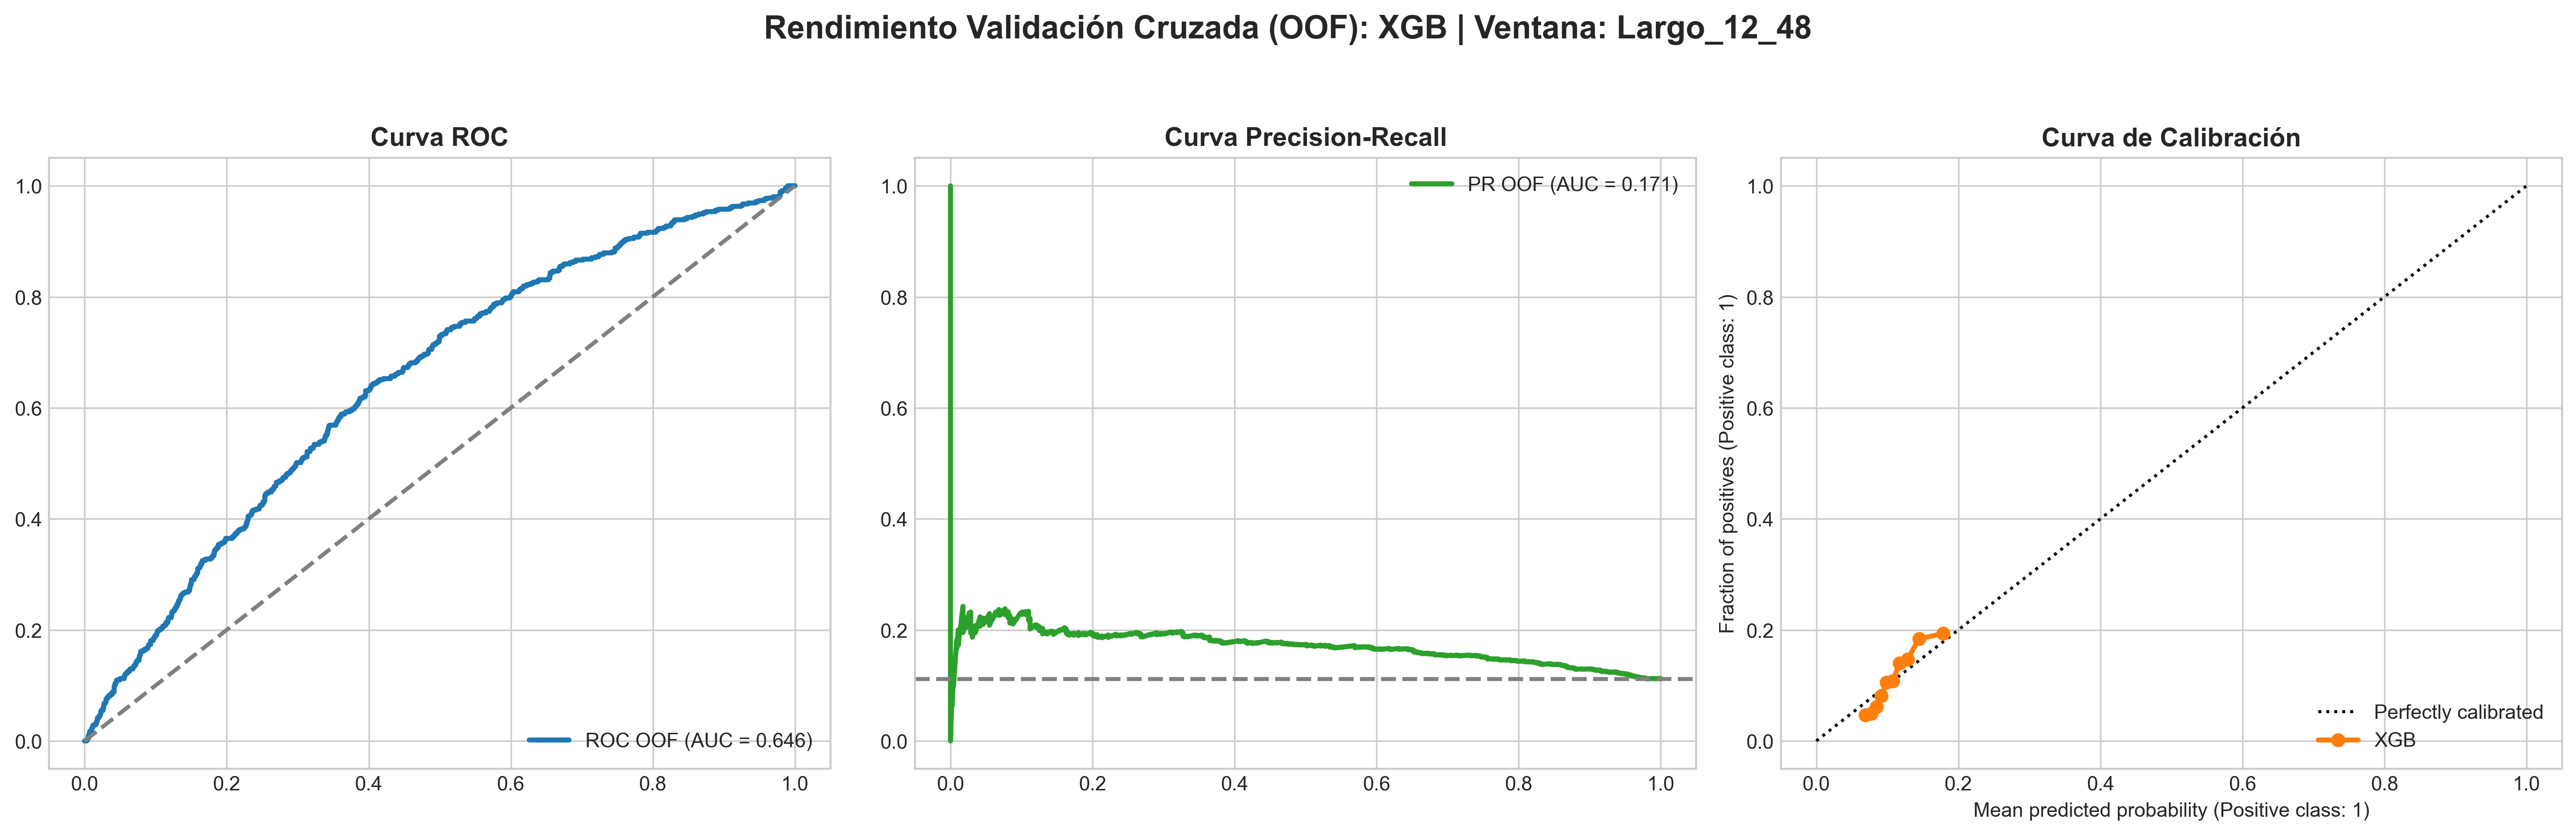
\includegraphics[width=\linewidth]{img/Grafica_OOF_Largo_12_48_XGB.png}\caption{XGBoost}\end{subfigure}\hfill
  \begin{subfigure}[t]{0.48\textwidth}\centering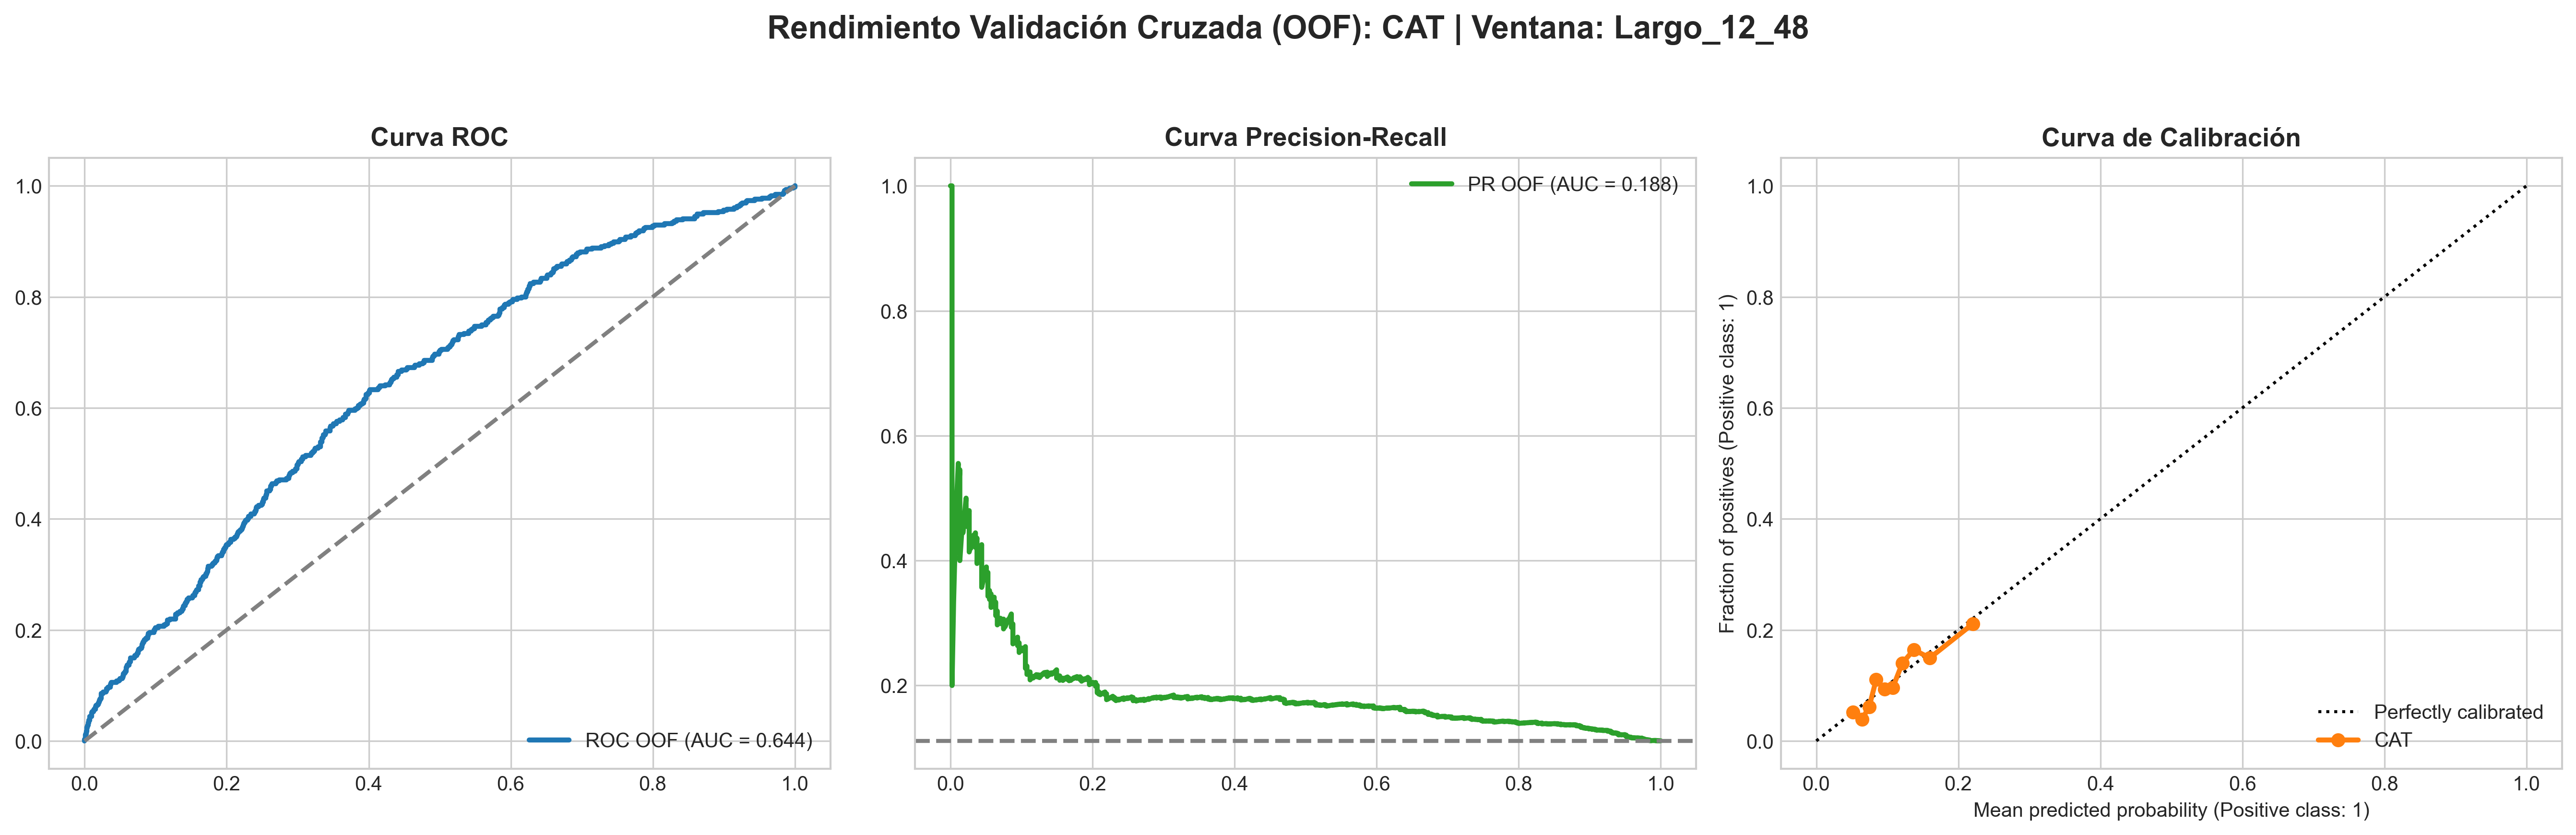
\includegraphics[width=\linewidth]{img/Grafica_OOF_Largo_12_48_CAT.png}\caption{CatBoost}\end{subfigure}\\[6pt]
  \begin{subfigure}[t]{0.48\textwidth}\centering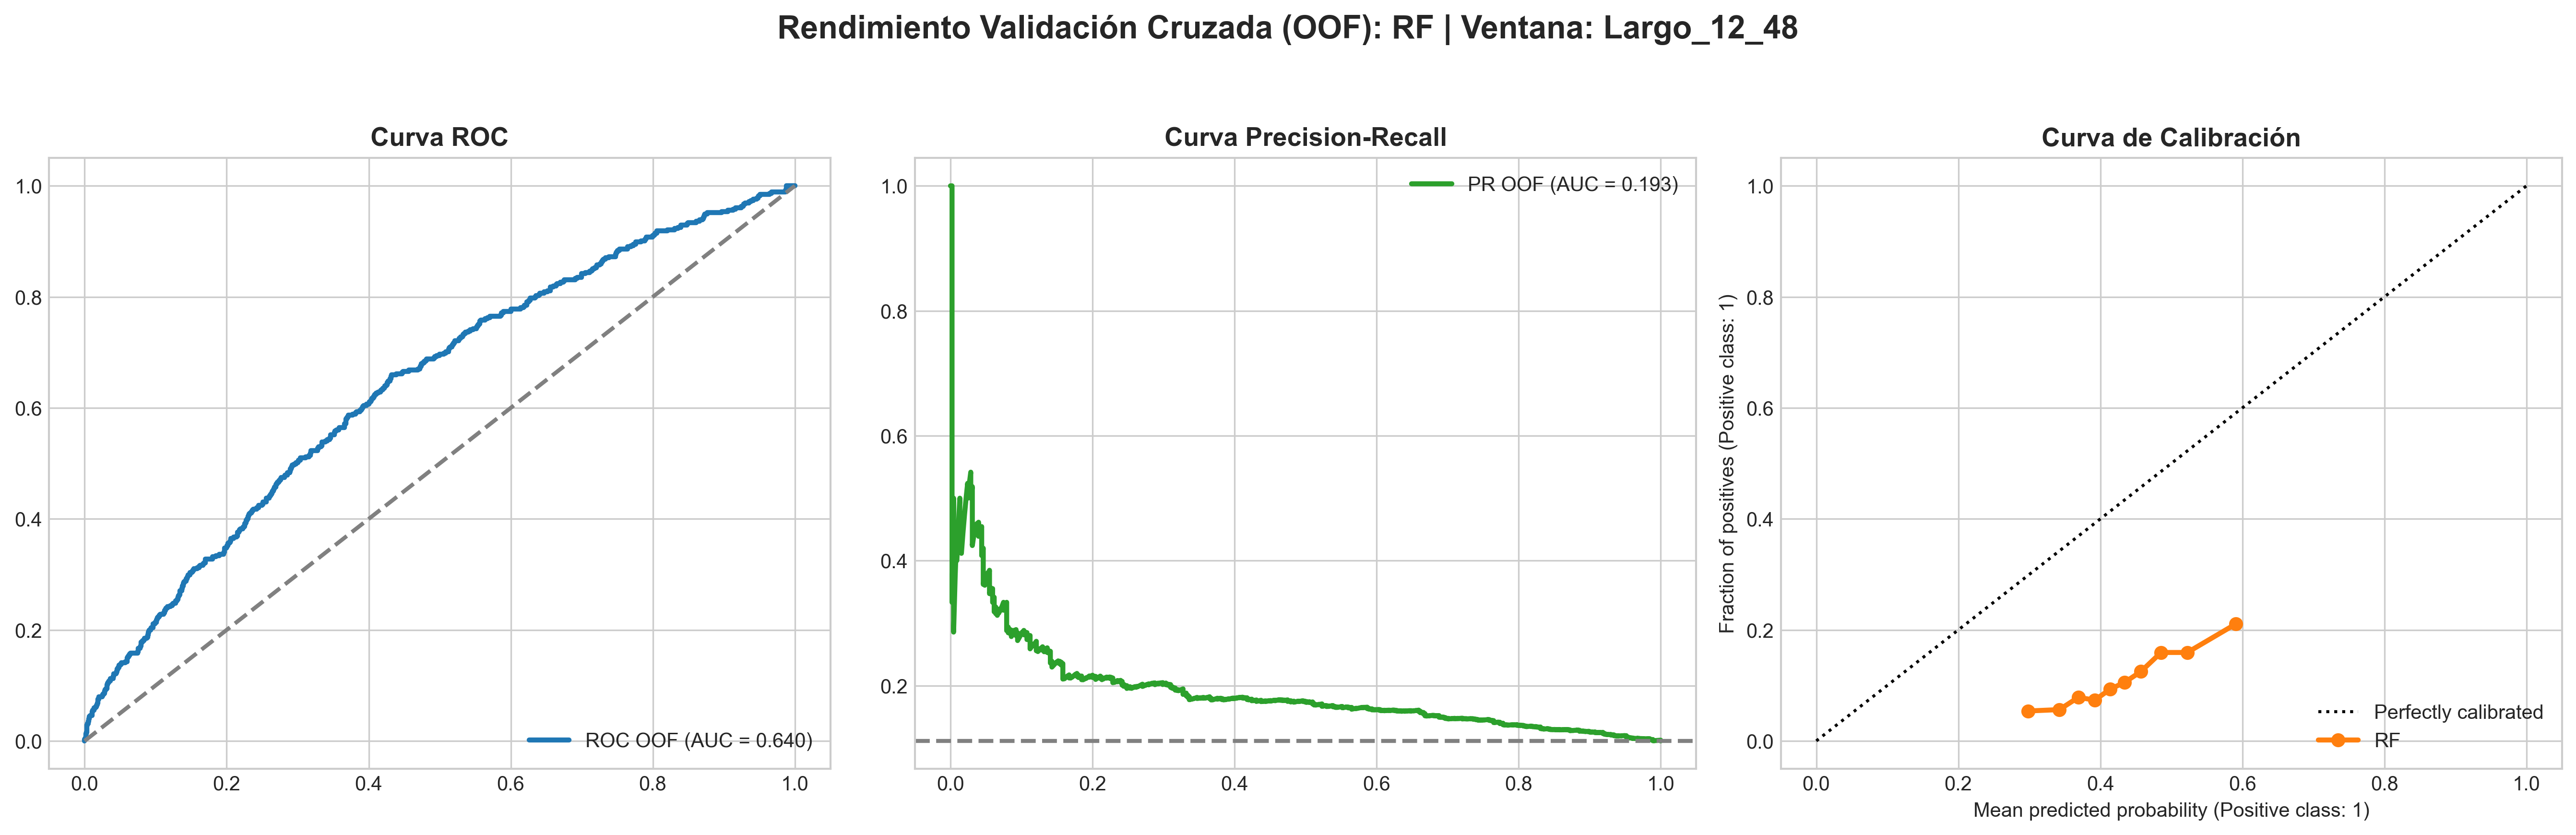
\includegraphics[width=\linewidth]{img/Grafica_OOF_Largo_12_48_RF.png}\caption{Random Forest}\end{subfigure}\hfill
  \begin{subfigure}[t]{0.48\textwidth}\centering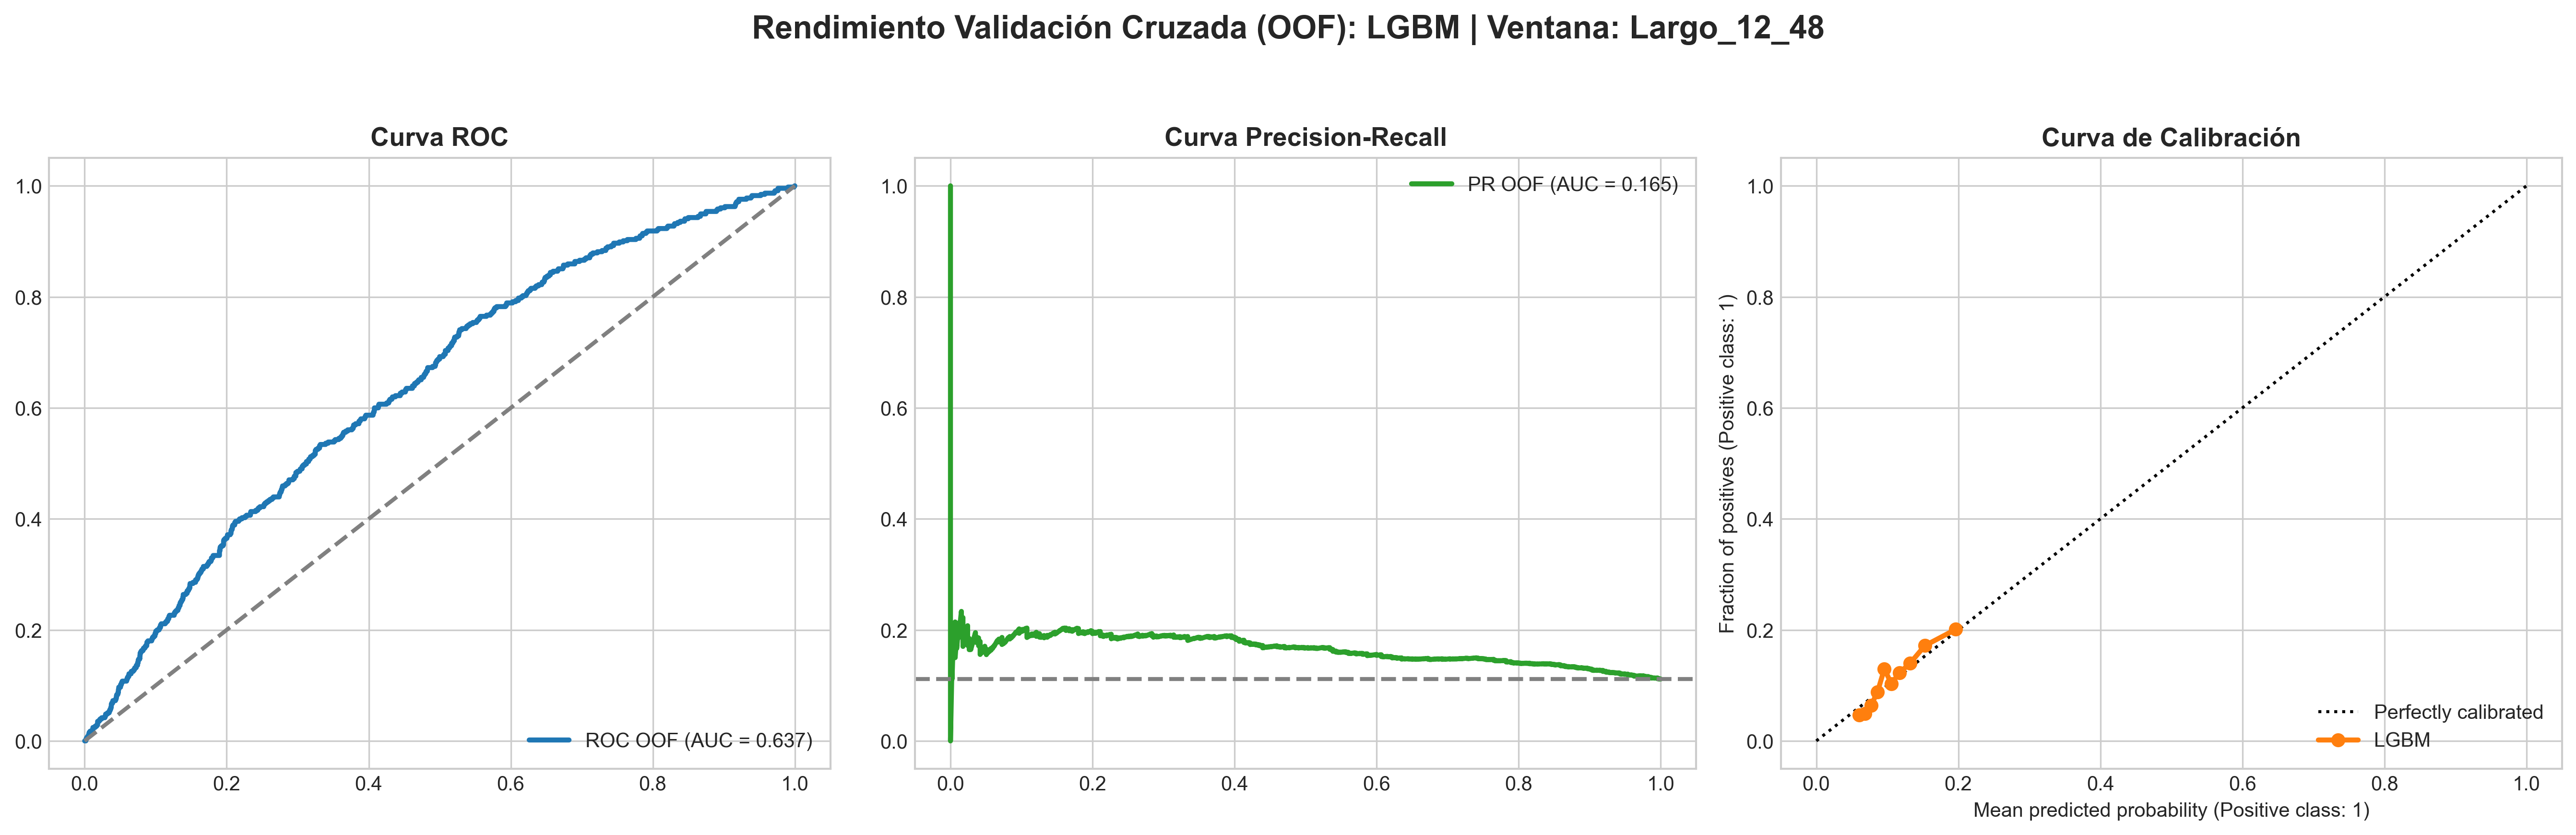
\includegraphics[width=\linewidth]{img/Grafica_OOF_Largo_12_48_LGBM.png}\caption{LightGBM}\end{subfigure}\\[6pt]
  \begin{subfigure}[t]{0.48\textwidth}\centering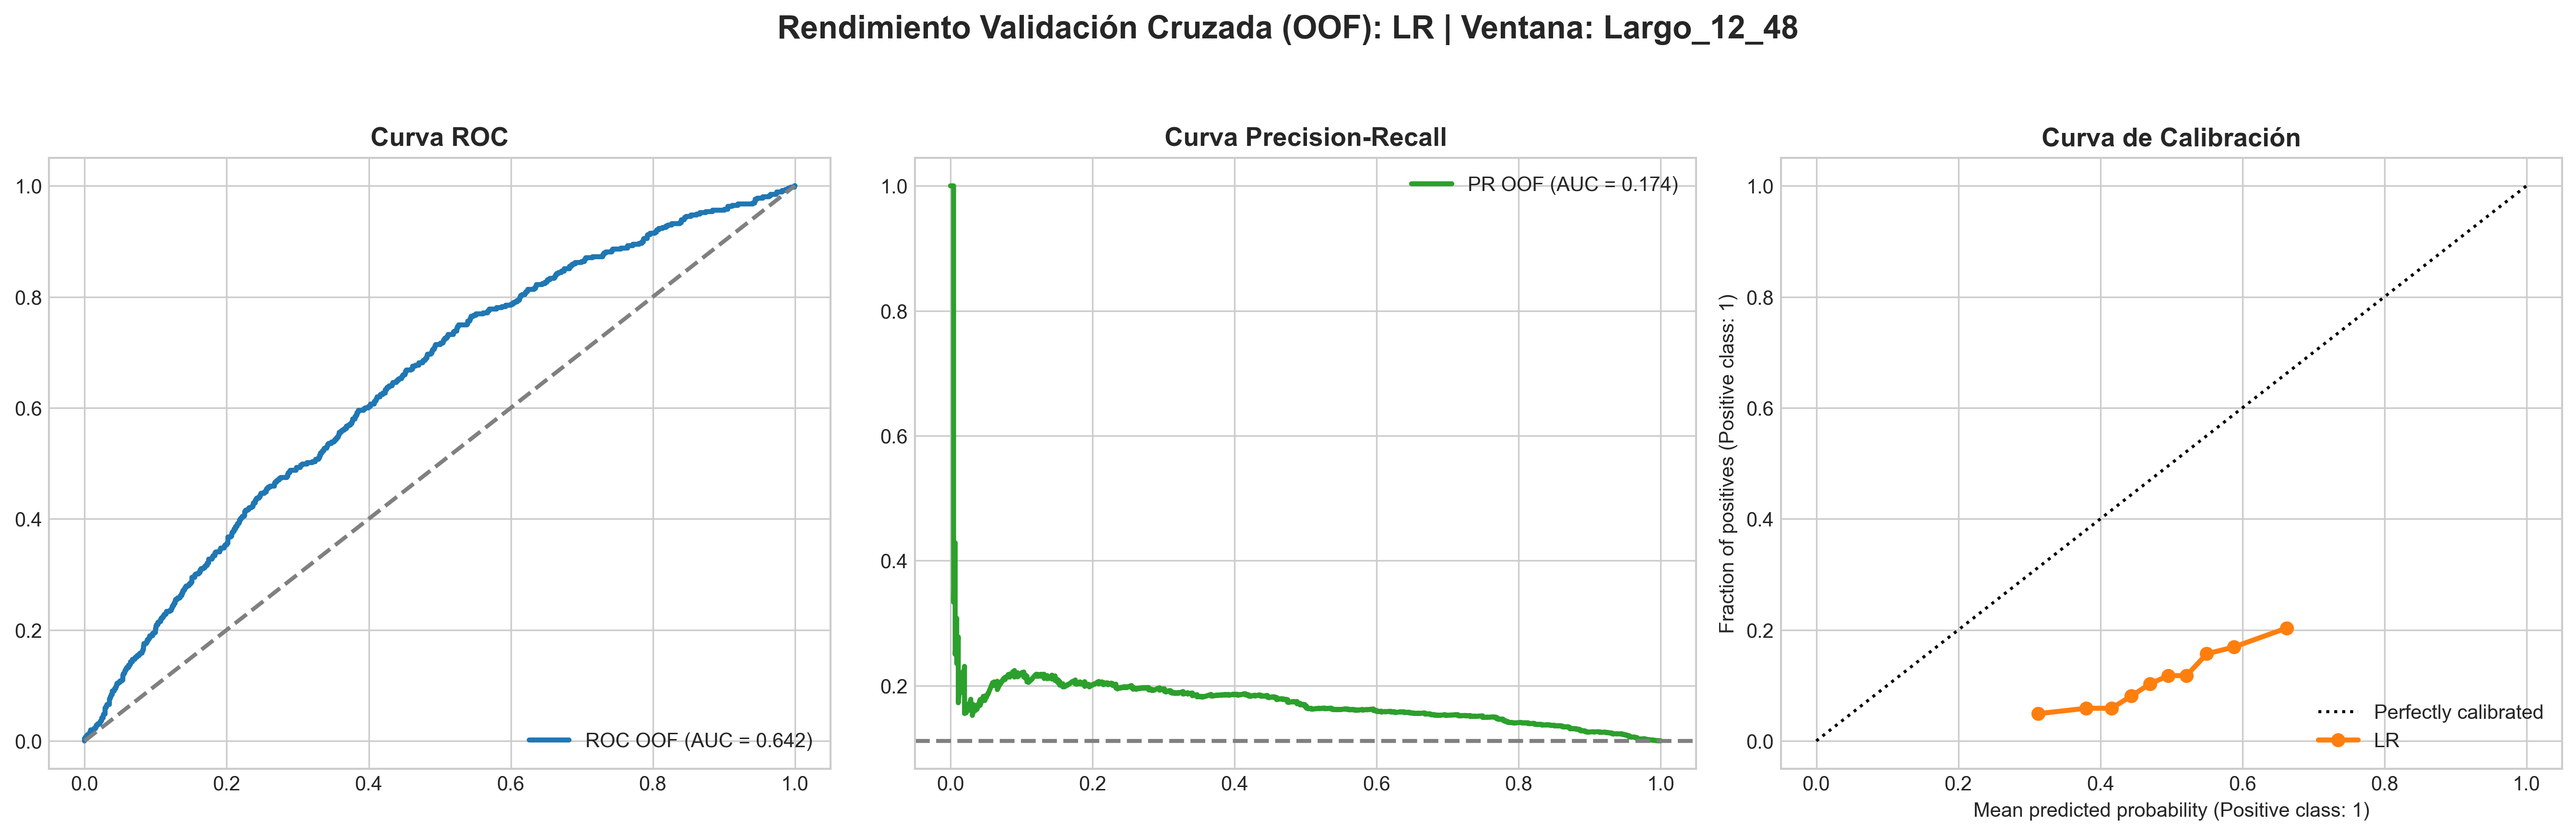
\includegraphics[width=\linewidth]{img/Grafica_OOF_Largo_12_48_LR.png}\caption{Regresión logística}\end{subfigure}\hfill
  \begin{subfigure}[t]{0.48\textwidth}\centering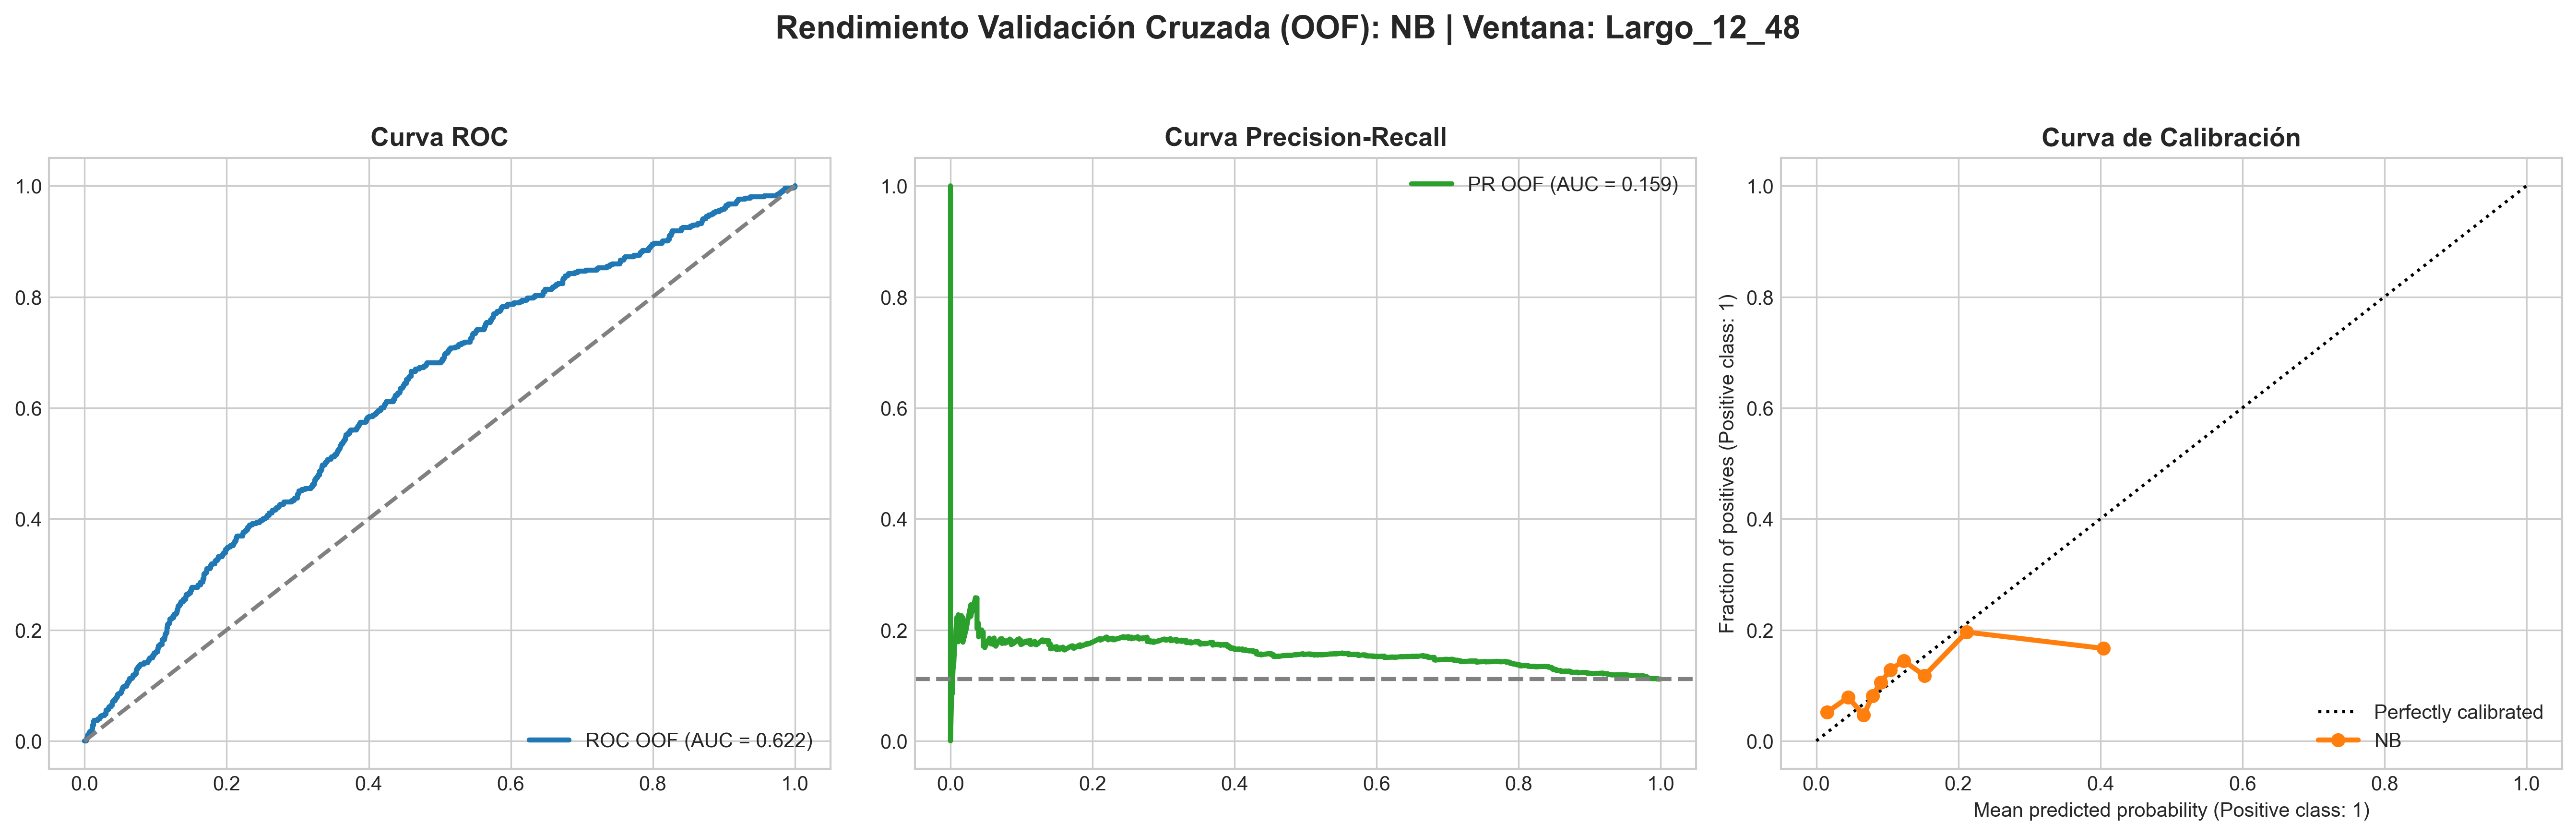
\includegraphics[width=\linewidth]{img/Grafica_OOF_Largo_12_48_NB.png}\caption{Naive Bayes}\end{subfigure}
  \caption{Rendimiento \textit{out-of-fold} de los modelos en la ventana larga (12--48\,h).}
  \label{fig:oof-largo}
\end{figure}
 
\subsubsection*{Comparación empírica de estrategias de calibración}

La figura~\ref{fig:calib} compara, sobre las probabilidades \textit{out-of-fold},
las tres estrategias de recalibración (sin calibrar, \textit{Platt} e isotónica)
mediante curvas de calibración, ECE y BSS. Solo el XGBoost de la ventana media
cumplió el criterio de mejora (menor ECE conservando BSS positivo) y fue
recalibrado; en el resto se conservó el modelo sin calibrar.
 
\begin{figure}[htbp]
  \centering
  \begin{subfigure}[t]{0.48\textwidth}\centering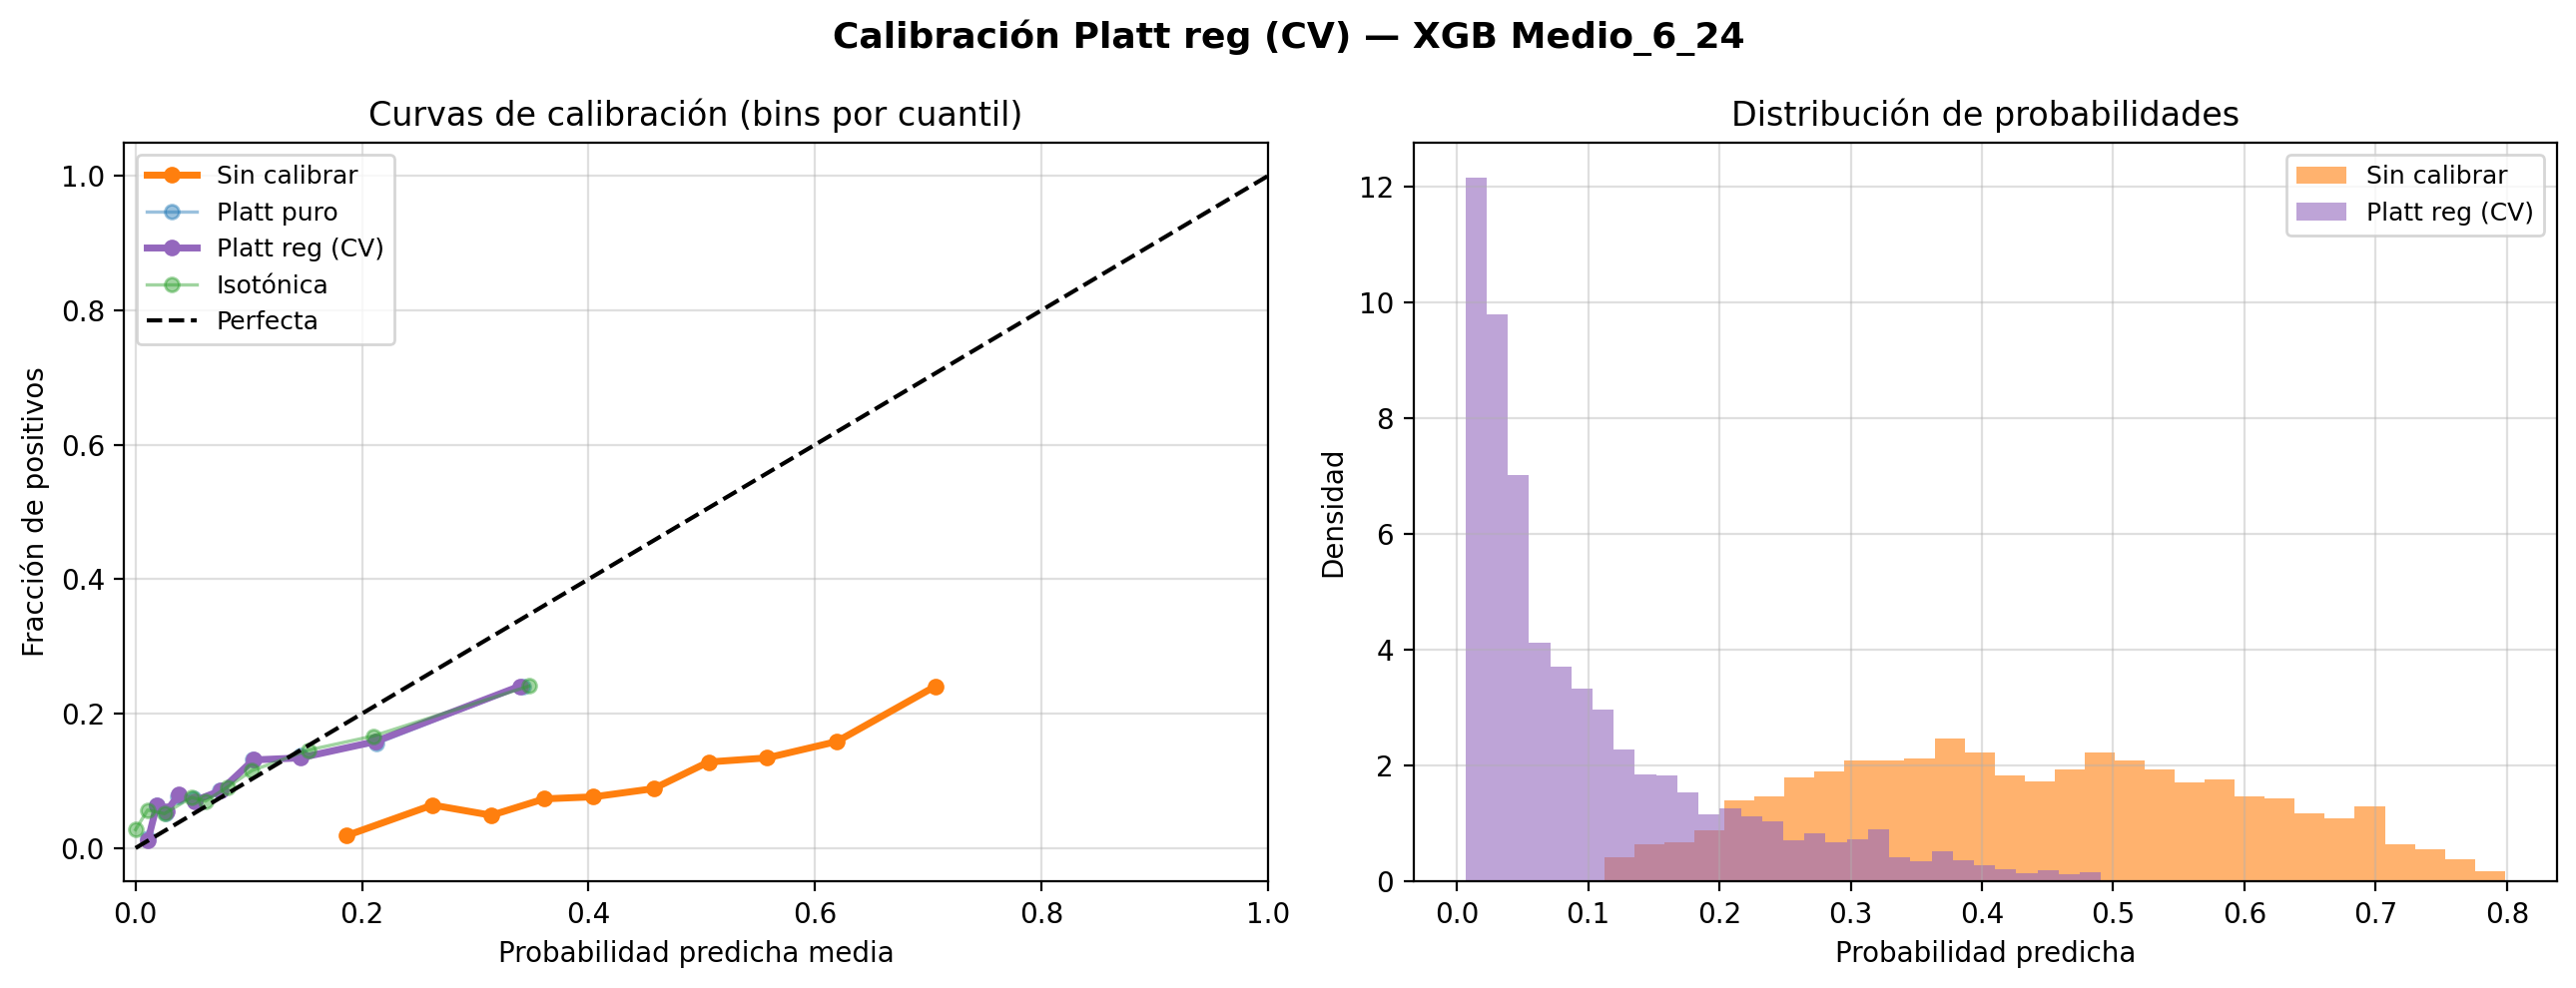
\includegraphics[width=\linewidth]{img/verificacion_calibracion_medio_xgb.png}\caption{XGBoost medio (recalibrado, Platt)}\end{subfigure}\hfill
  \begin{subfigure}[t]{0.48\textwidth}\centering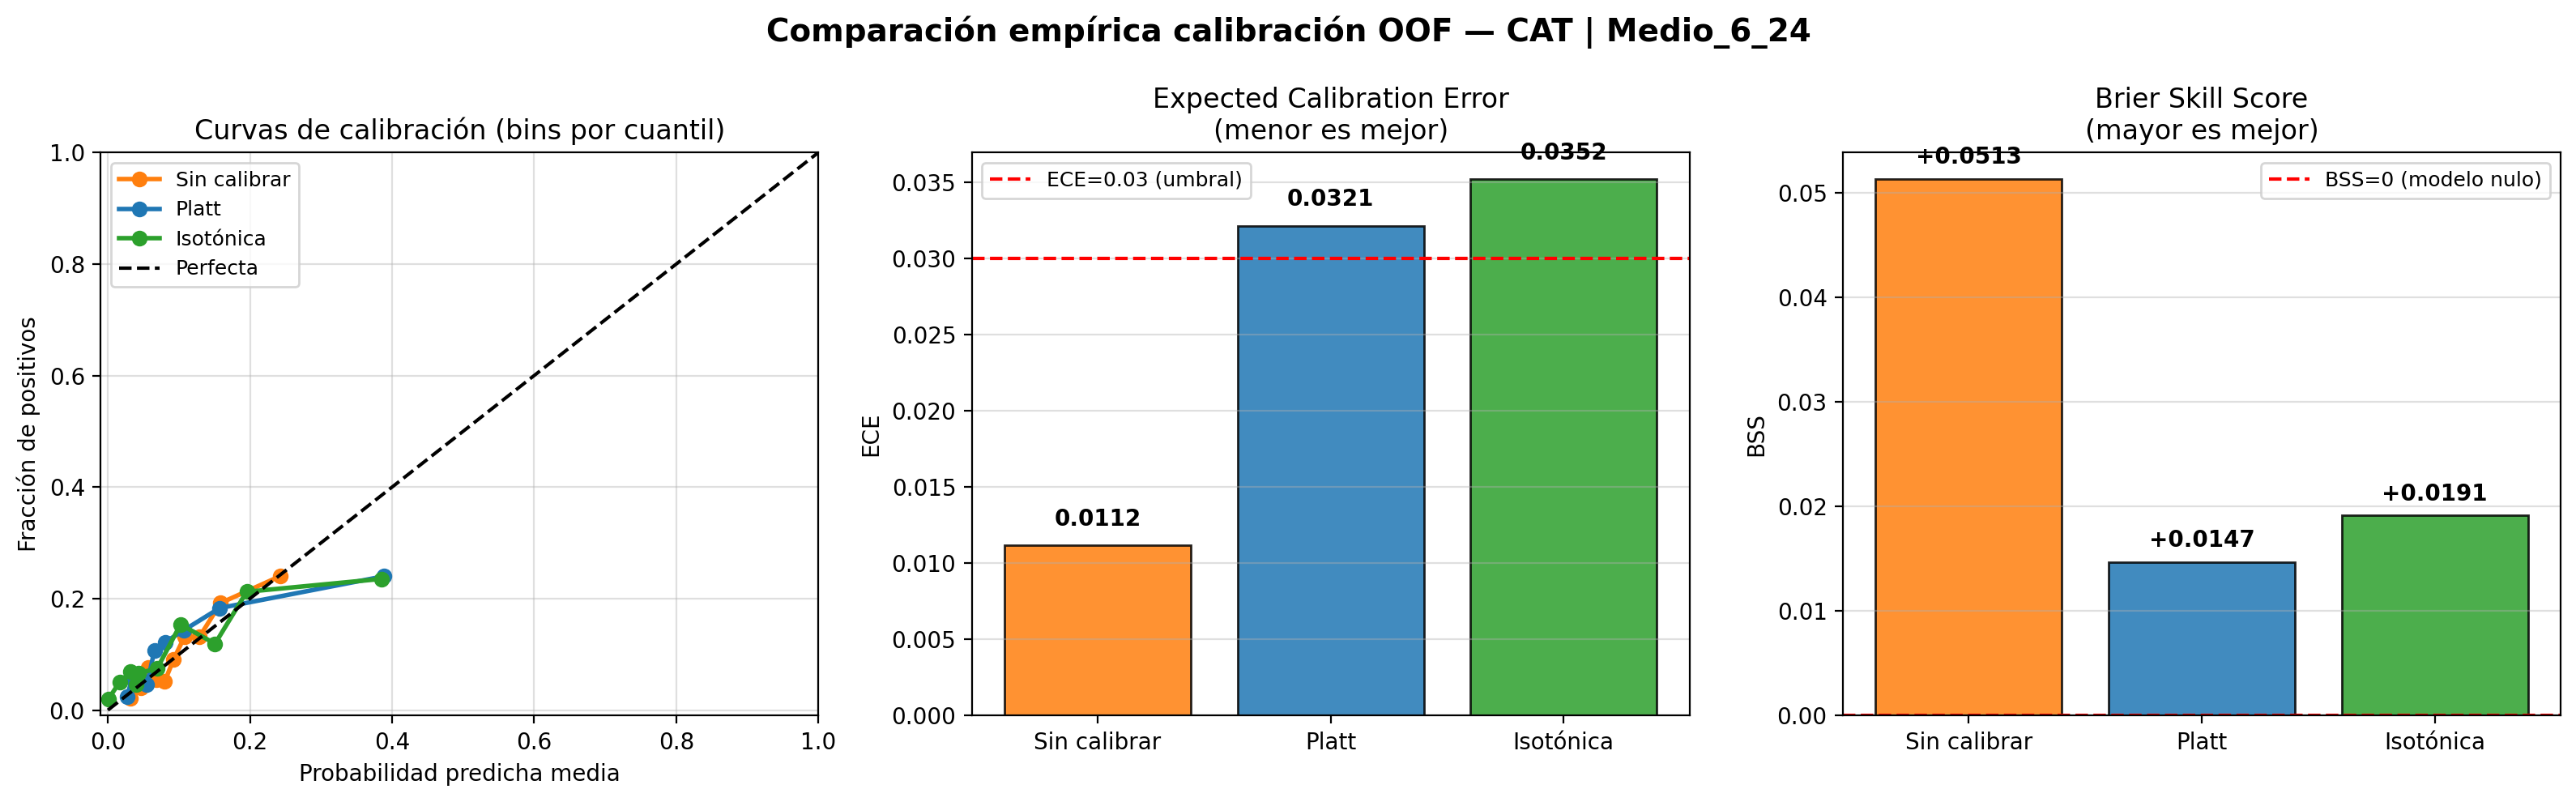
\includegraphics[width=\linewidth]{img/calibracion_comparativa_medio_cat.png}\caption{CatBoost medio (sin calibrar)}\end{subfigure}\\[6pt]
  \begin{subfigure}[t]{0.48\textwidth}\centering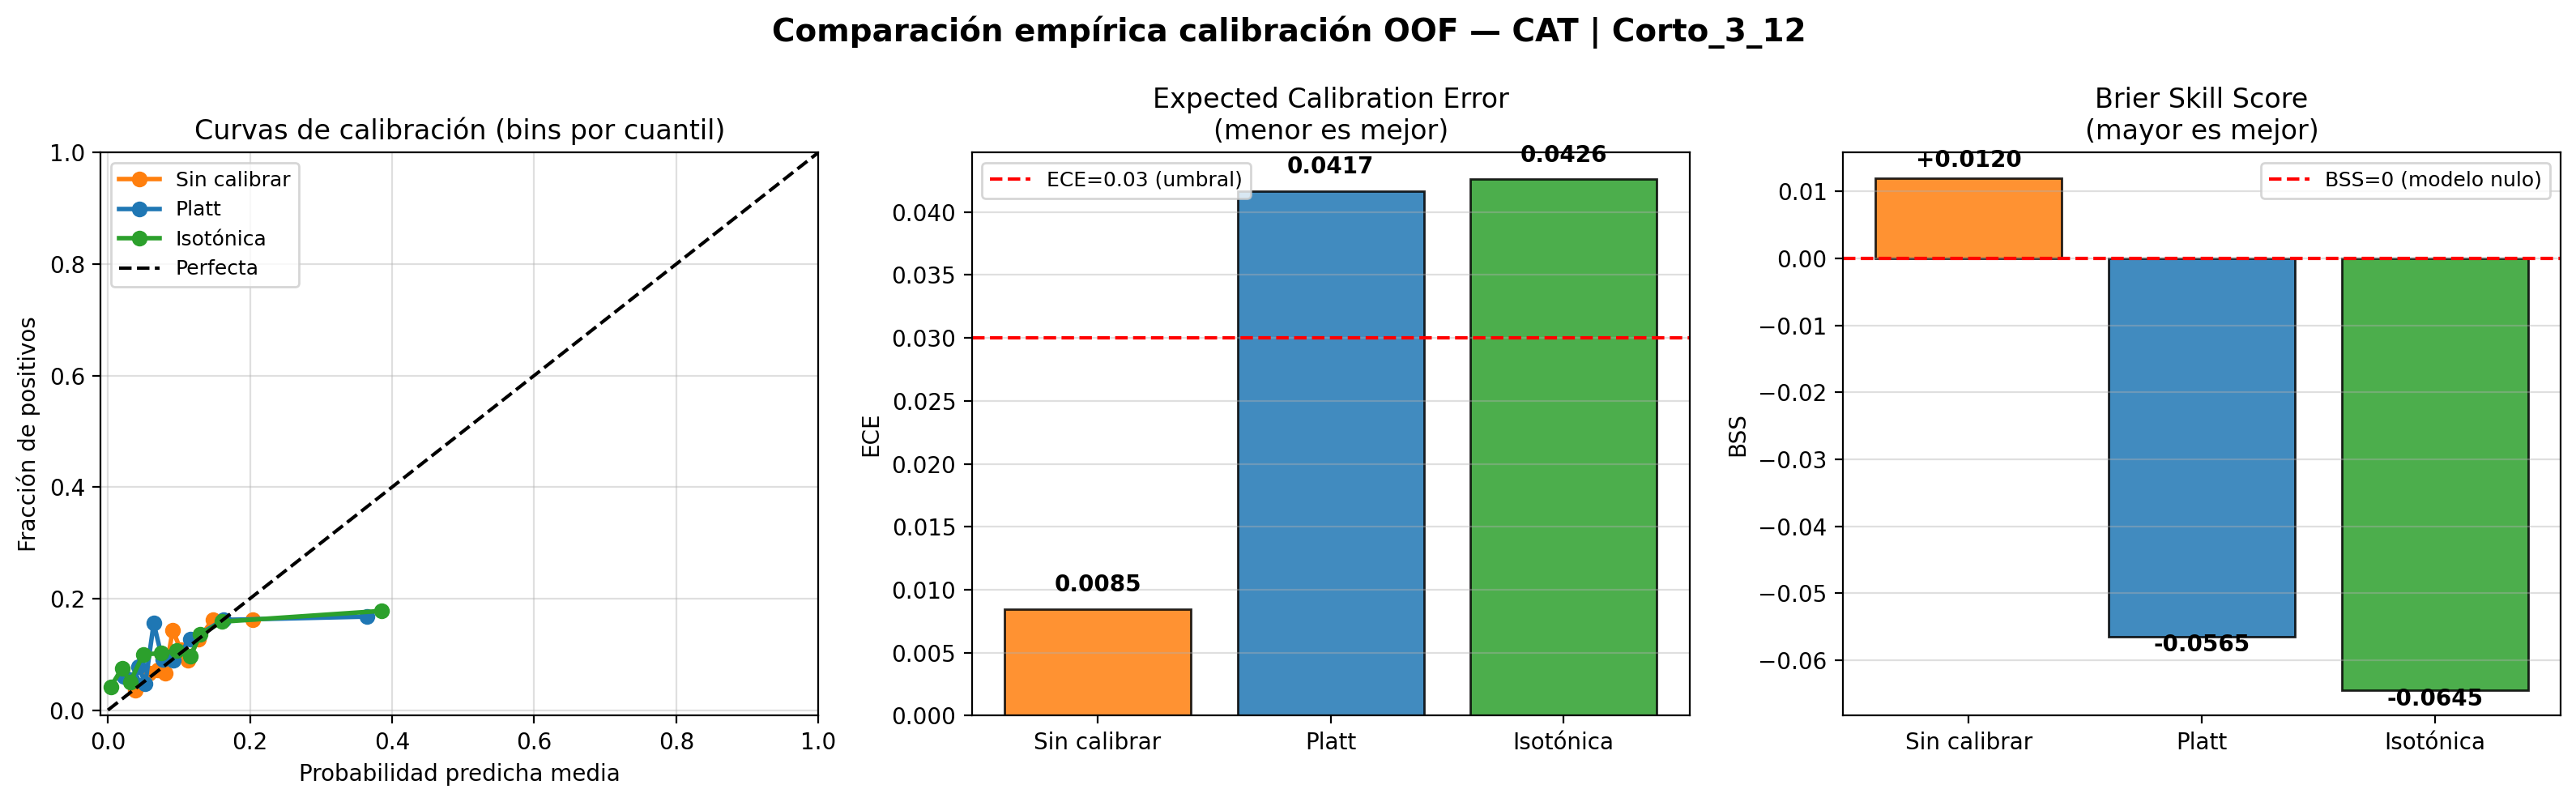
\includegraphics[width=\linewidth]{img/calibracion_comparativa_corto_cat.png}\caption{CatBoost corto (sin calibrar)}\end{subfigure}\hfill
  \begin{subfigure}[t]{0.48\textwidth}\centering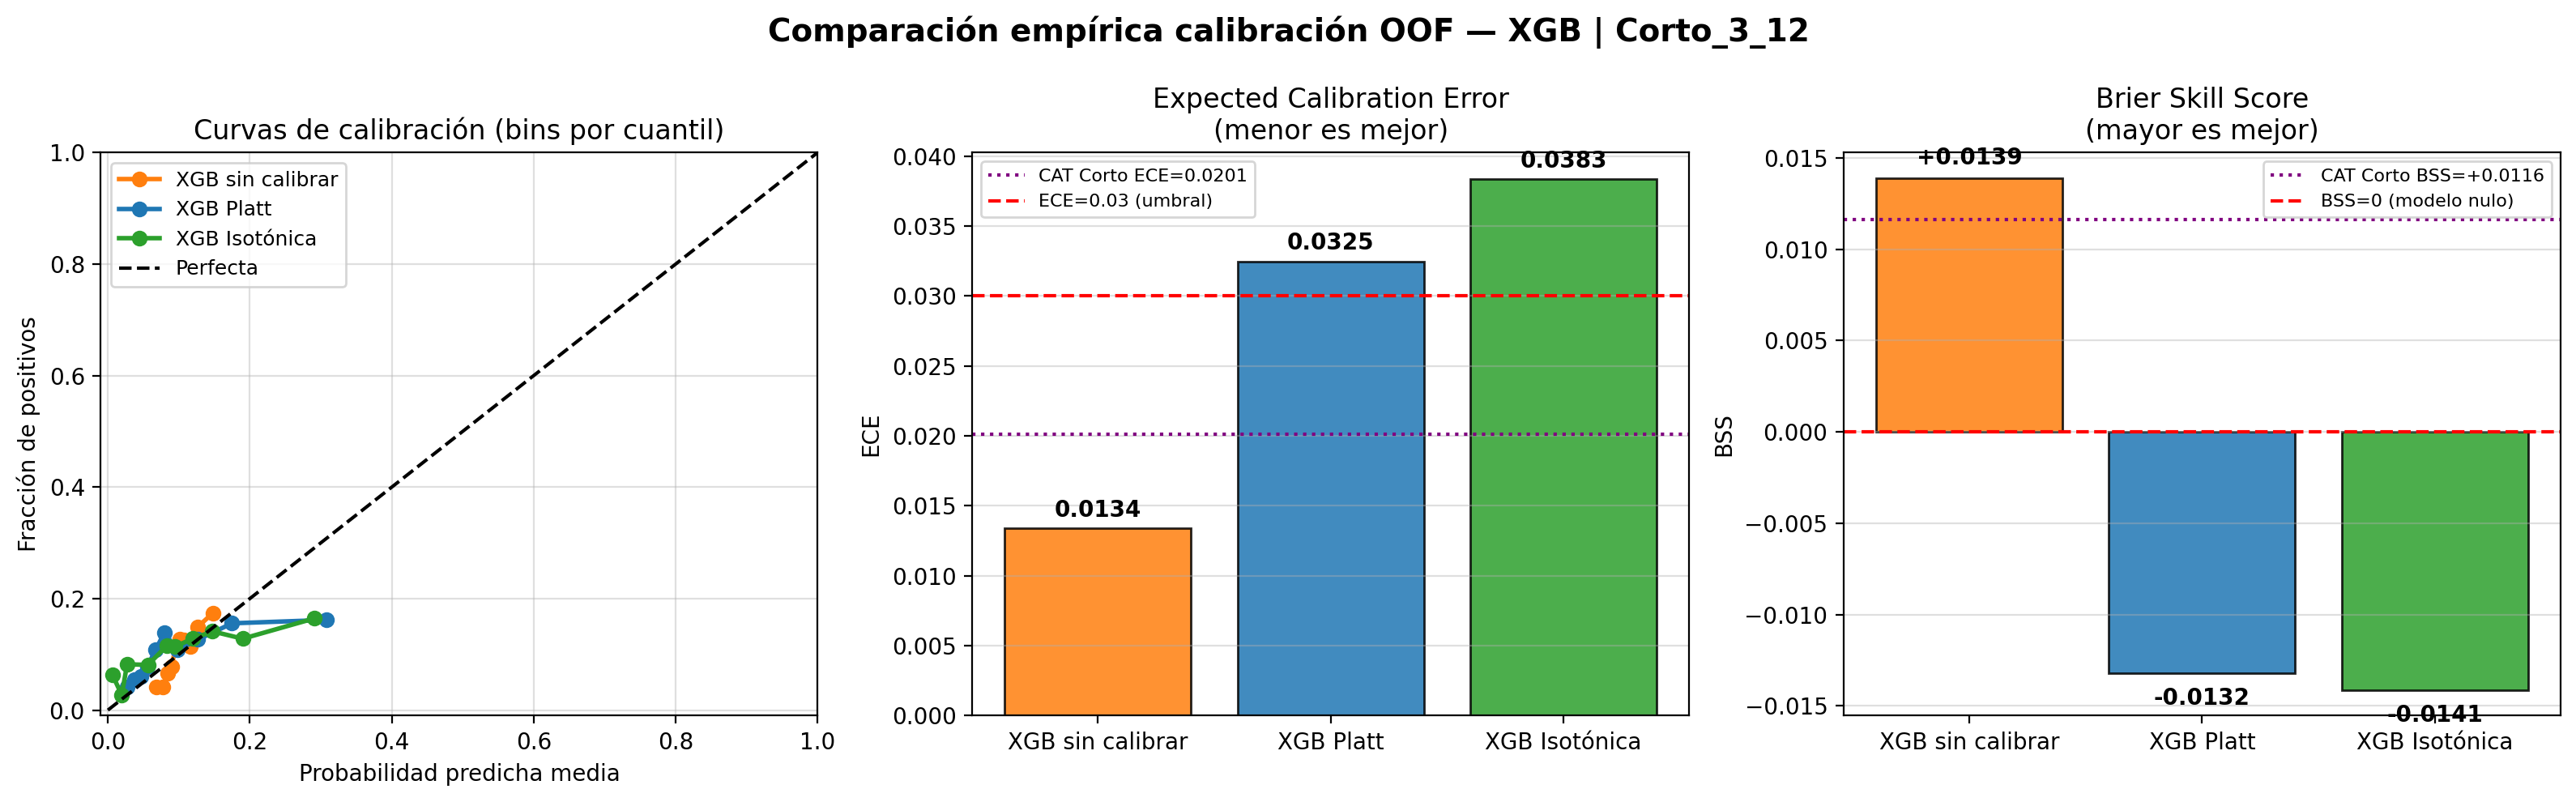
\includegraphics[width=\linewidth]{img/calibracion_comparativa_corto_xgb.png}\caption{XGBoost corto (sin calibrar)}\end{subfigure}\\[6pt]
  \begin{subfigure}[t]{0.48\textwidth}\centering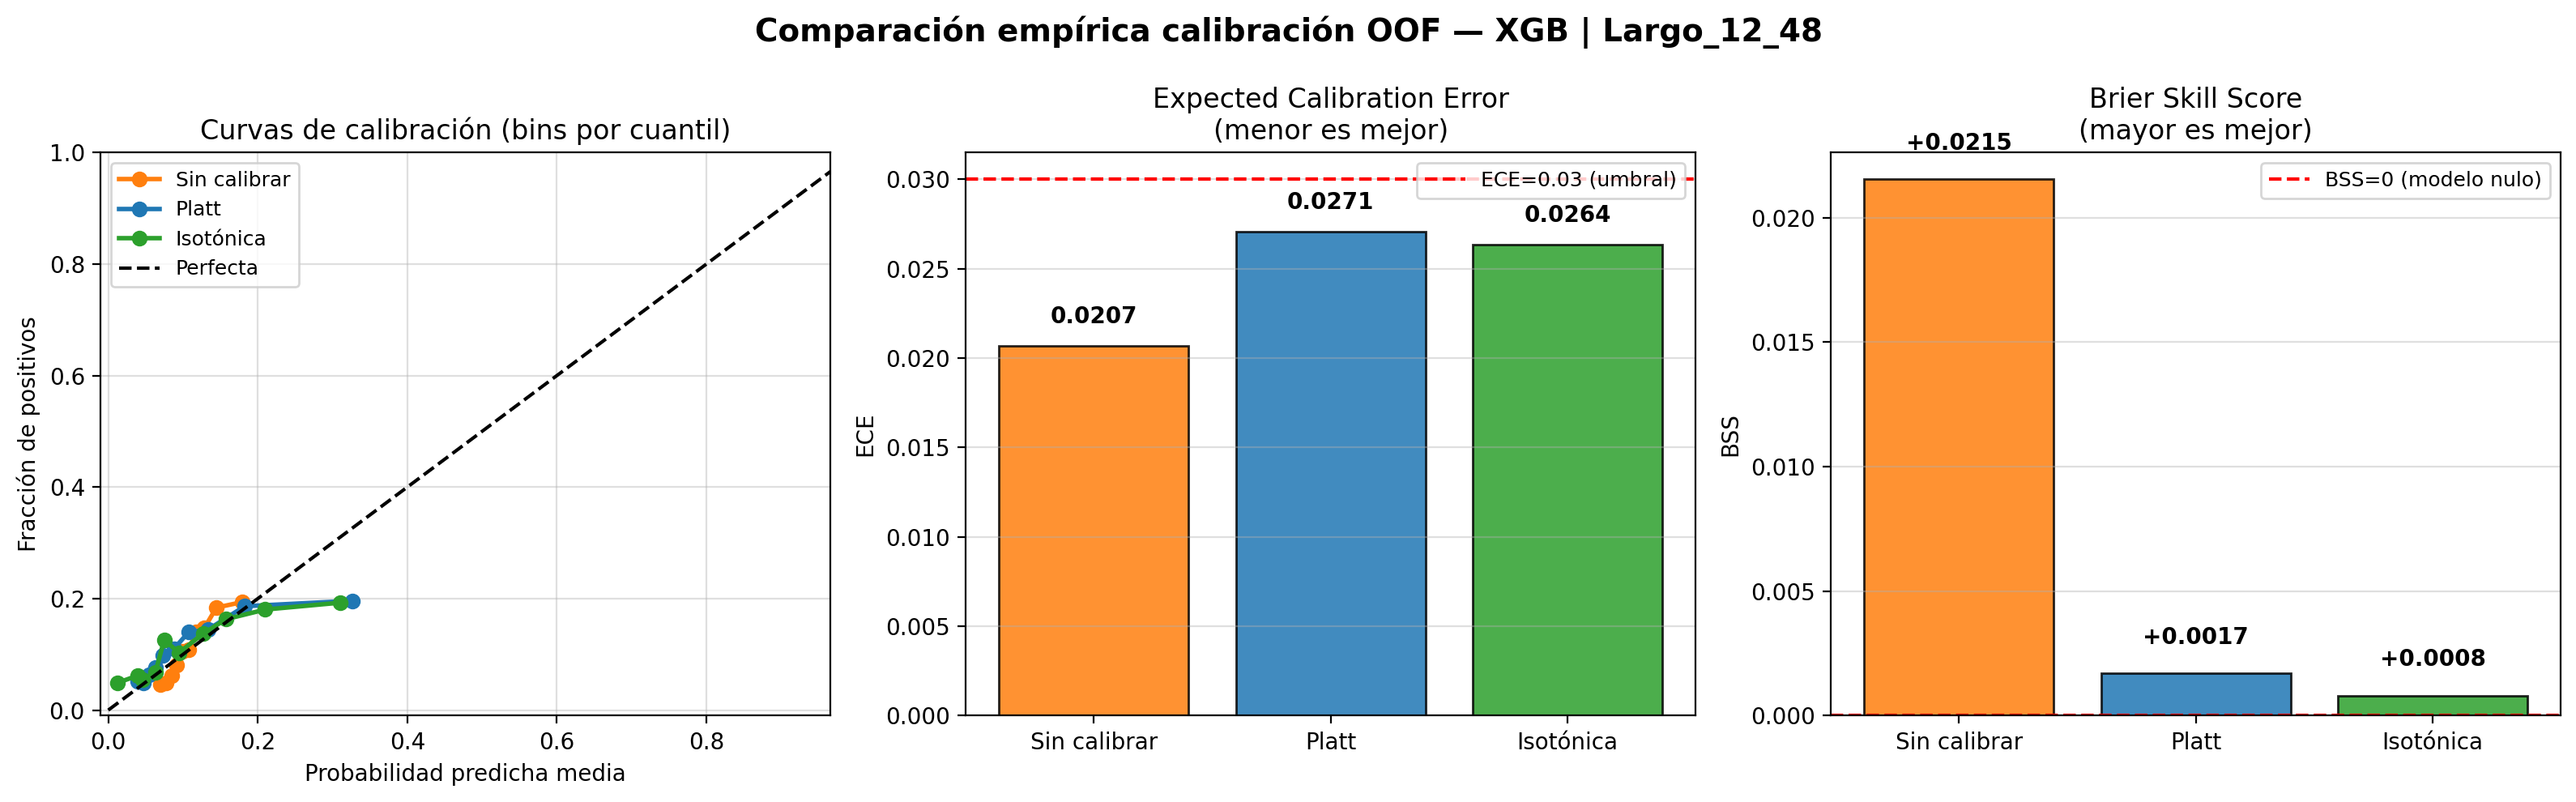
\includegraphics[width=\linewidth]{img/calibracion_comparativa_largo_xgb.png}\caption{XGBoost largo (sin calibrar)}\end{subfigure}
  \caption{Comparación de calibración (sin calibrar / Platt / isotónica) con ECE y BSS por método.}
  \label{fig:calib}
\end{figure}
 
\subsubsection*{Diagramas SHAP internos (MIMIC-IV)}

Las figuras~\ref{fig:shap-corto}--\ref{fig:shap-largo} recogen los diagramas
\textit{beeswarm} de SHAP de todos los modelos por ventana sobre MIMIC-IV,
empleados como capa de auditoría de la coherencia fisiopatológica.
 
\begin{figure}[htbp]
  \centering
  \begin{subfigure}[t]{0.48\textwidth}\centering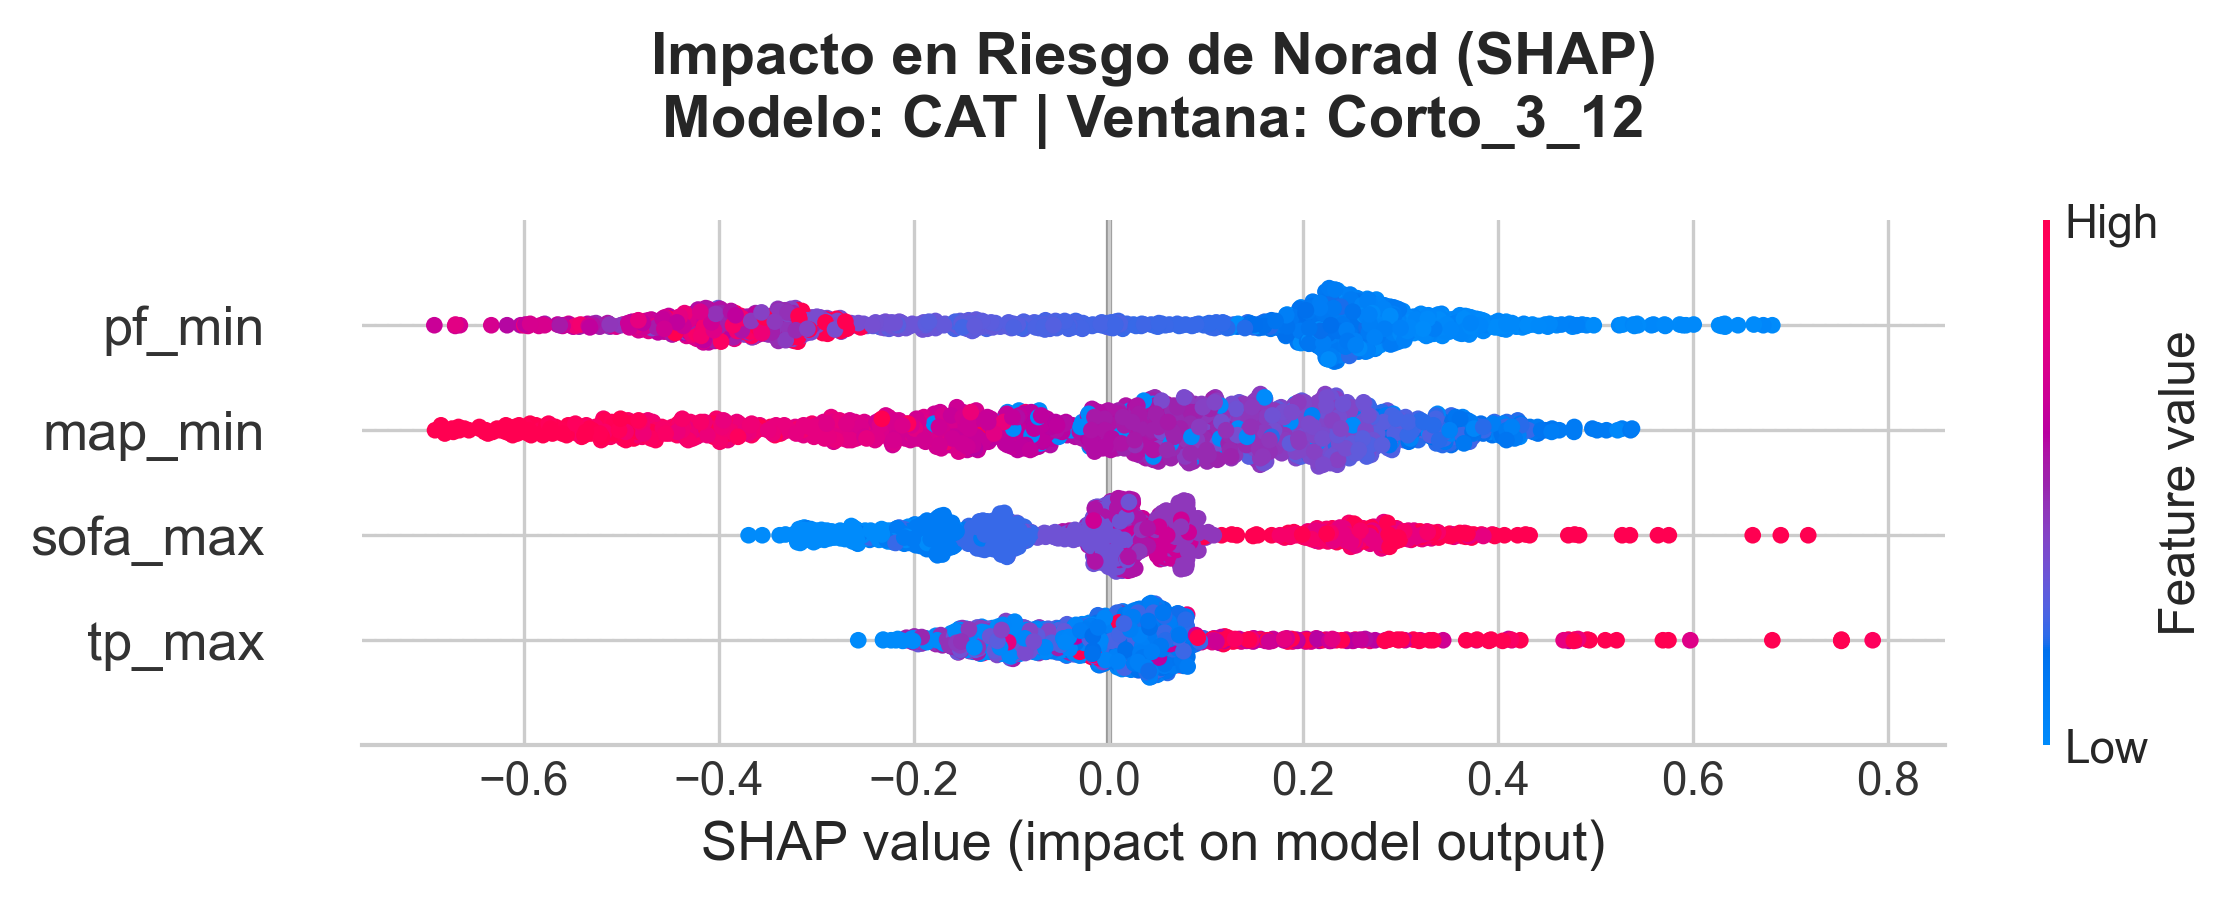
\includegraphics[width=\linewidth]{img/SHAP_Corto_3_12_CAT.png}\caption{CatBoost}\end{subfigure}\hfill
  \begin{subfigure}[t]{0.48\textwidth}\centering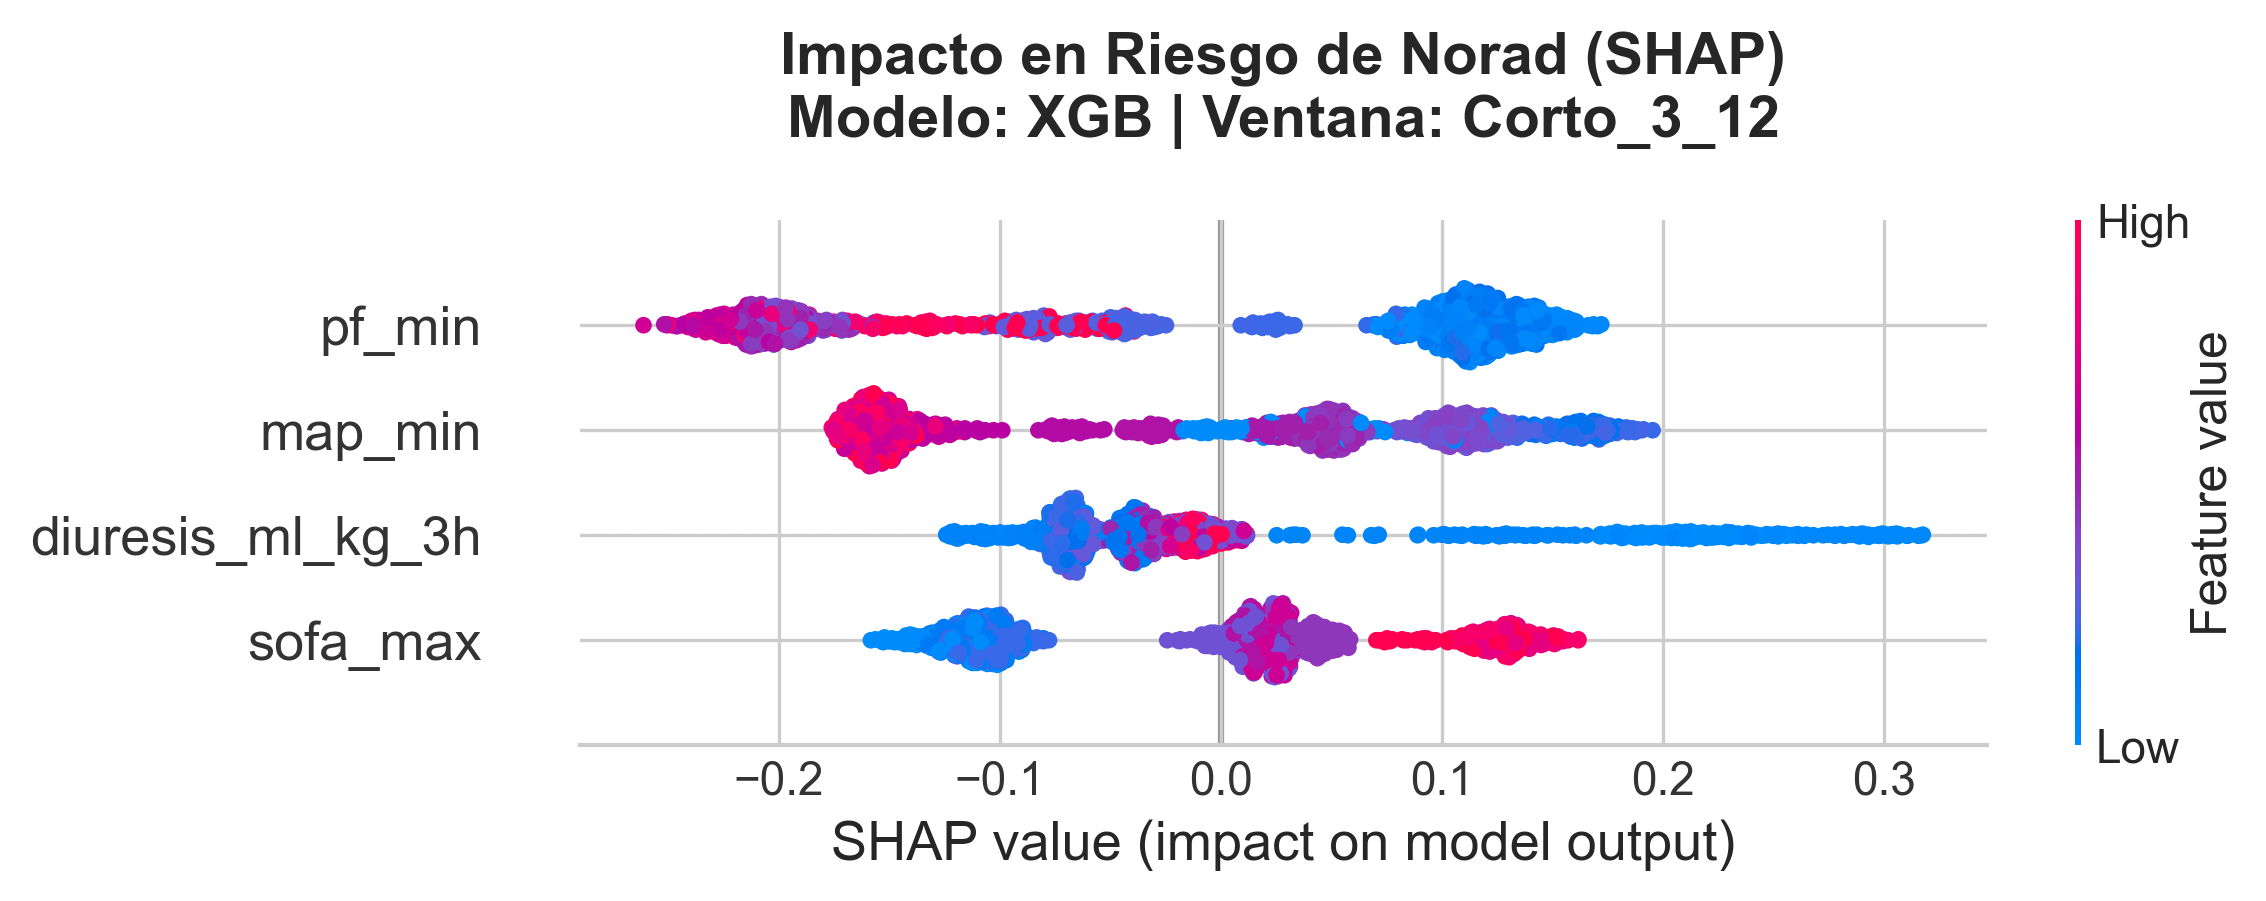
\includegraphics[width=\linewidth]{img/SHAP_Corto_3_12_XGB.png}\caption{XGBoost}\end{subfigure}\\[6pt]
  \begin{subfigure}[t]{0.48\textwidth}\centering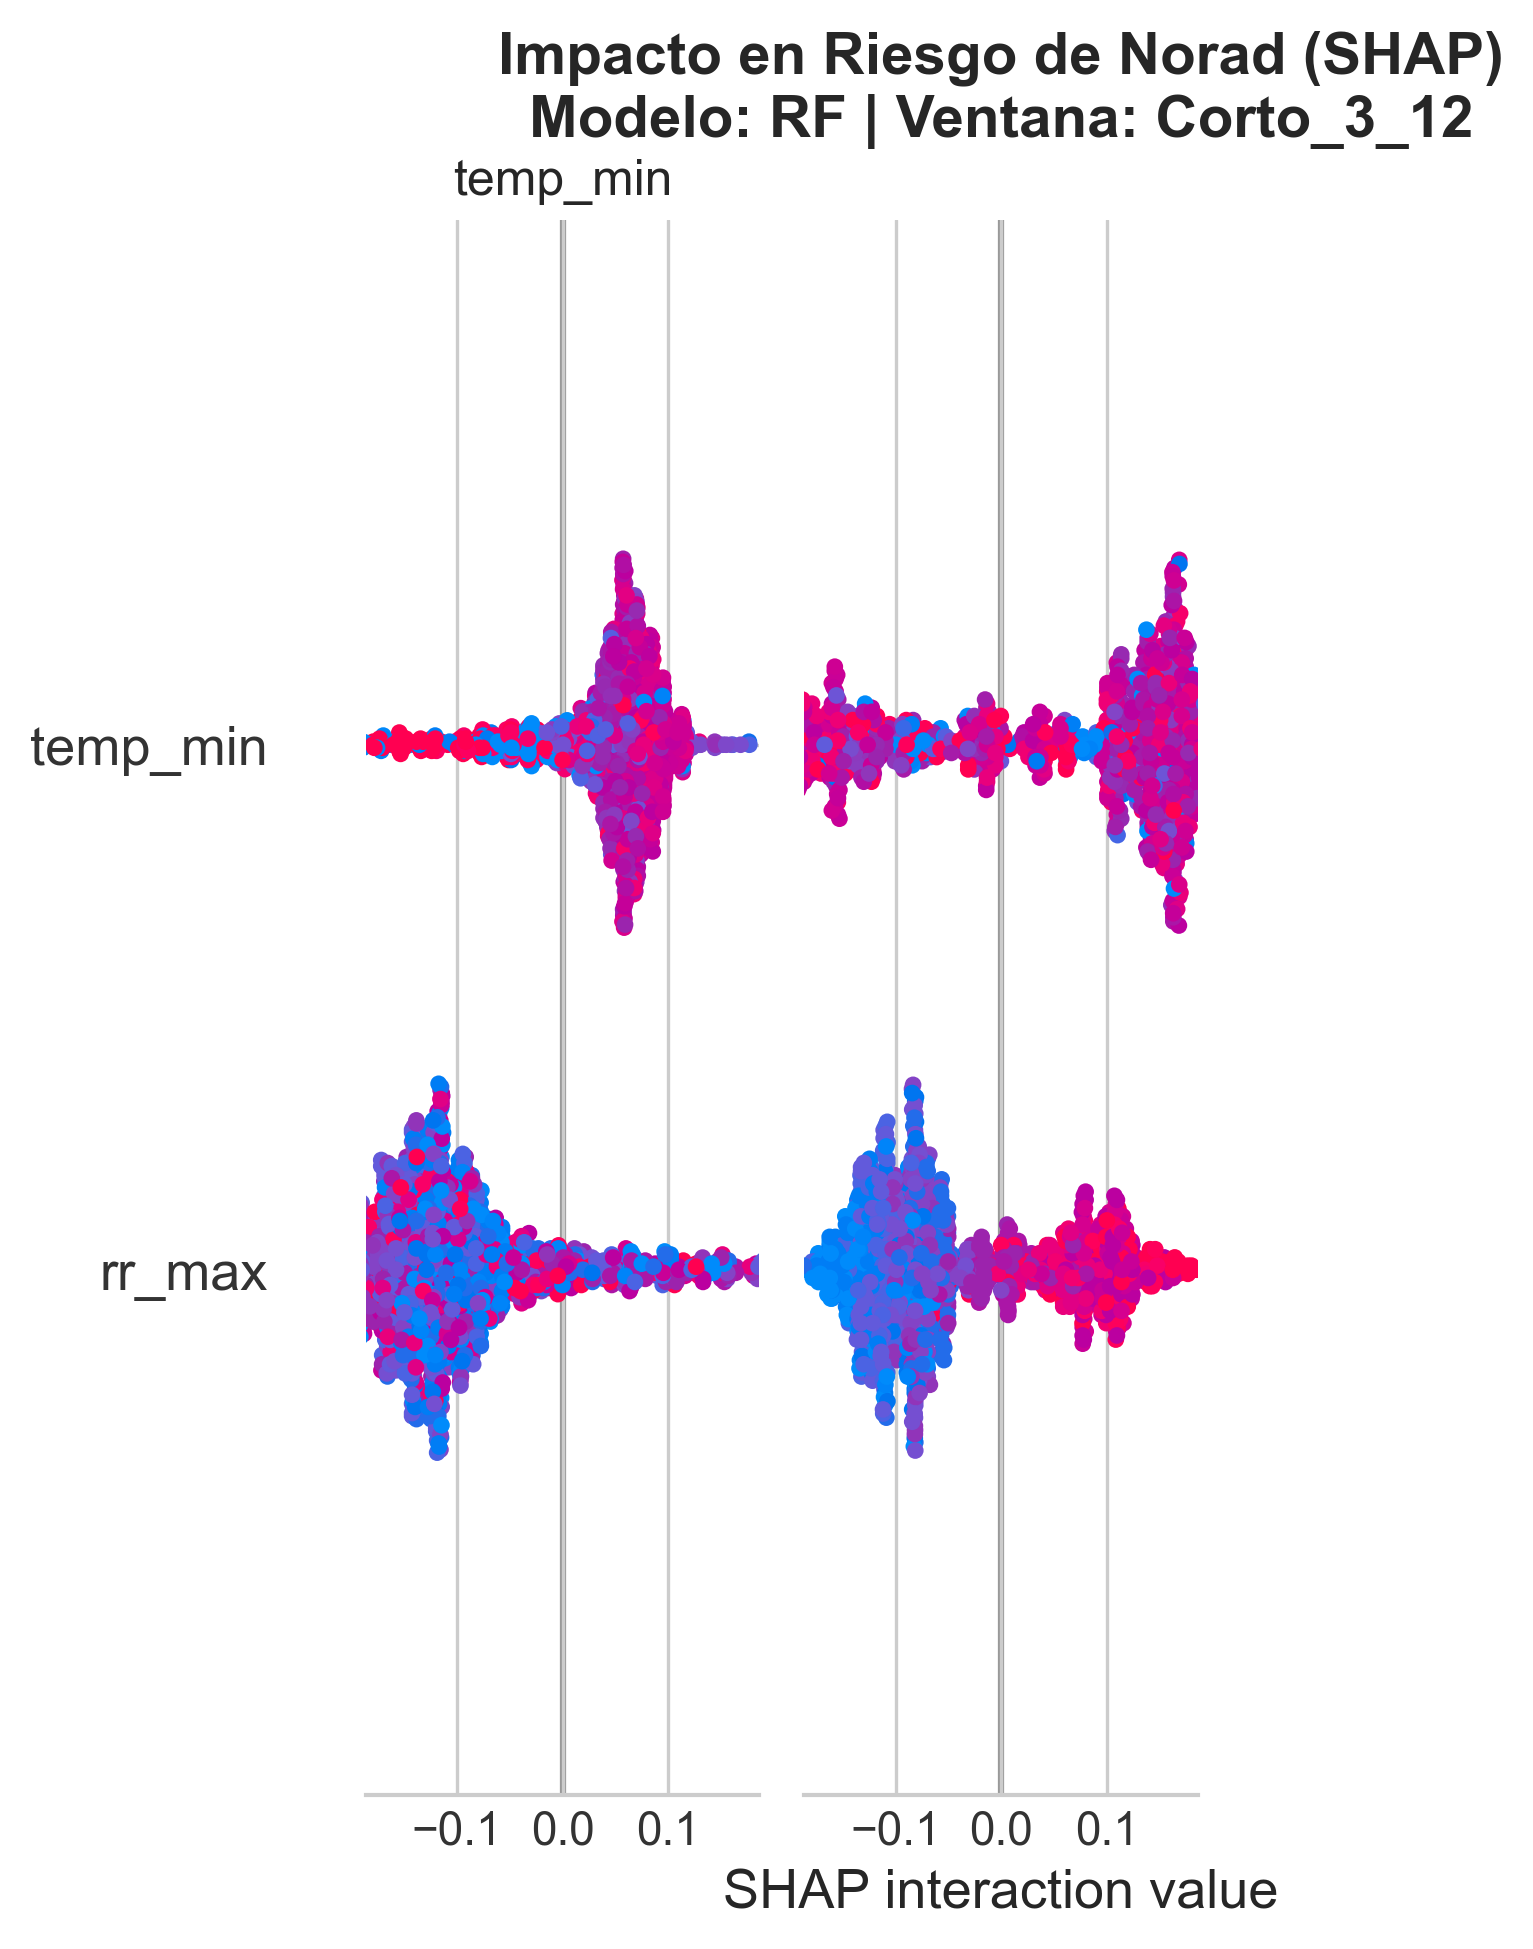
\includegraphics[width=\linewidth]{img/SHAP_Corto_3_12_RF.png}\caption{Random Forest}\end{subfigure}\hfill
  \begin{subfigure}[t]{0.48\textwidth}\centering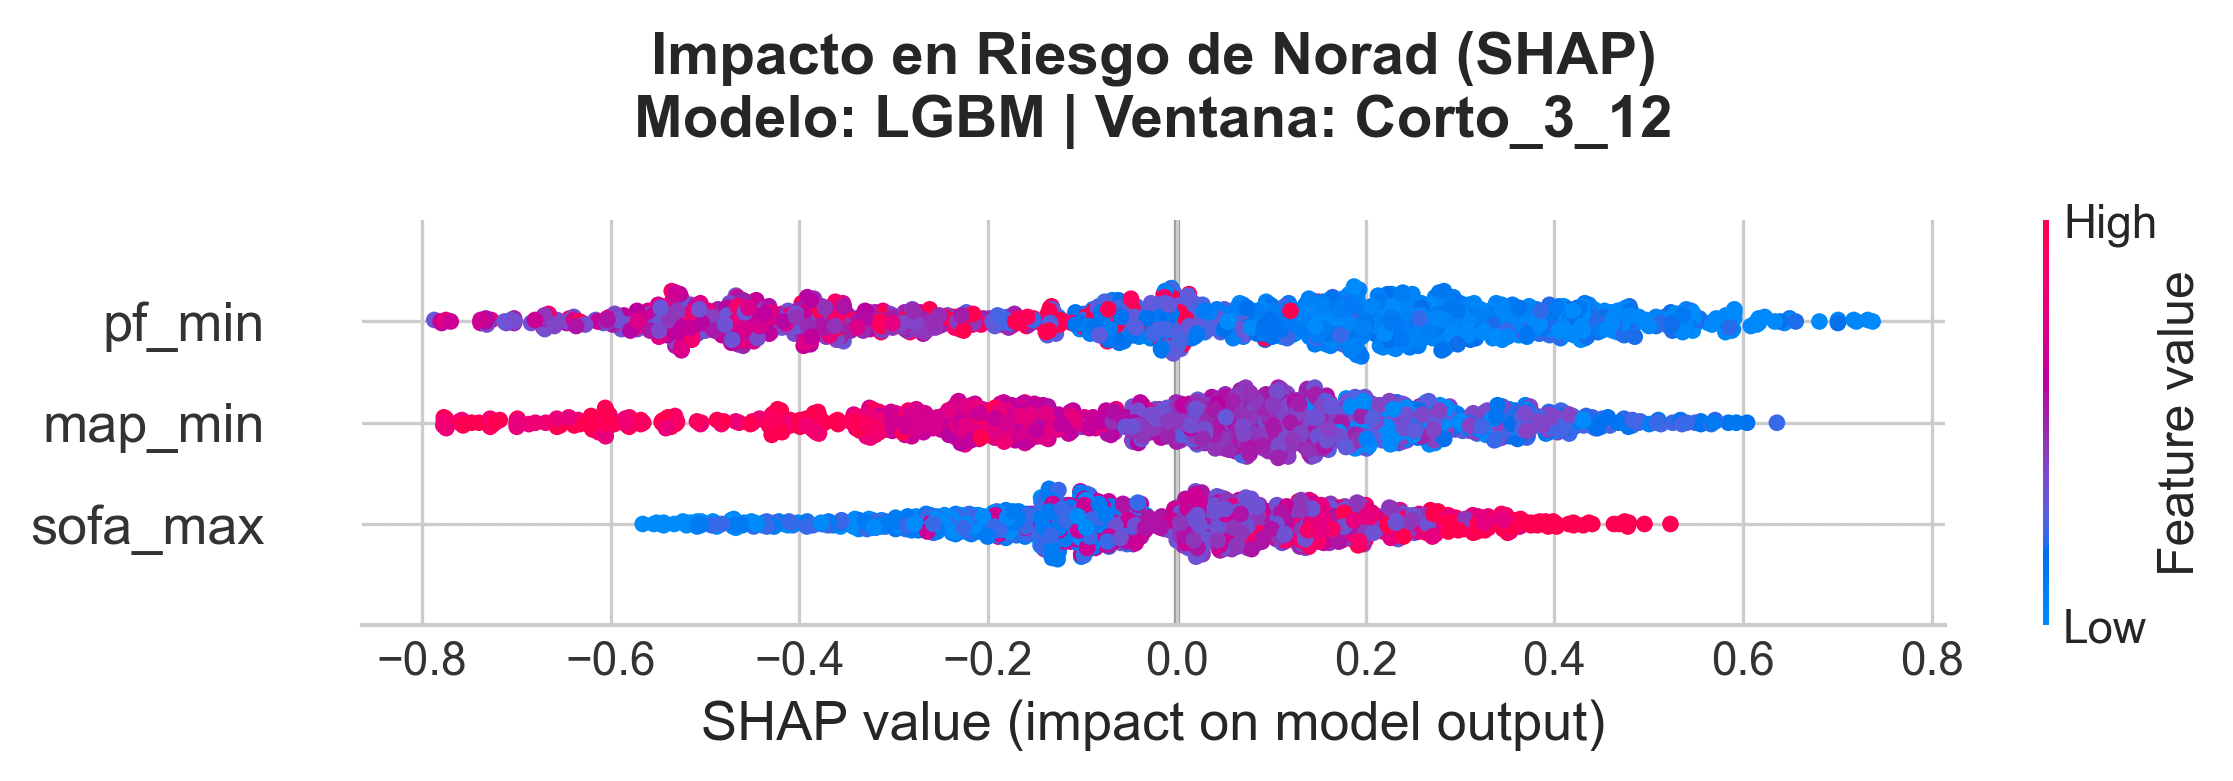
\includegraphics[width=\linewidth]{img/SHAP_Corto_3_12_LGBM.png}\caption{LightGBM}\end{subfigure}\\[6pt]
  \begin{subfigure}[t]{0.48\textwidth}\centering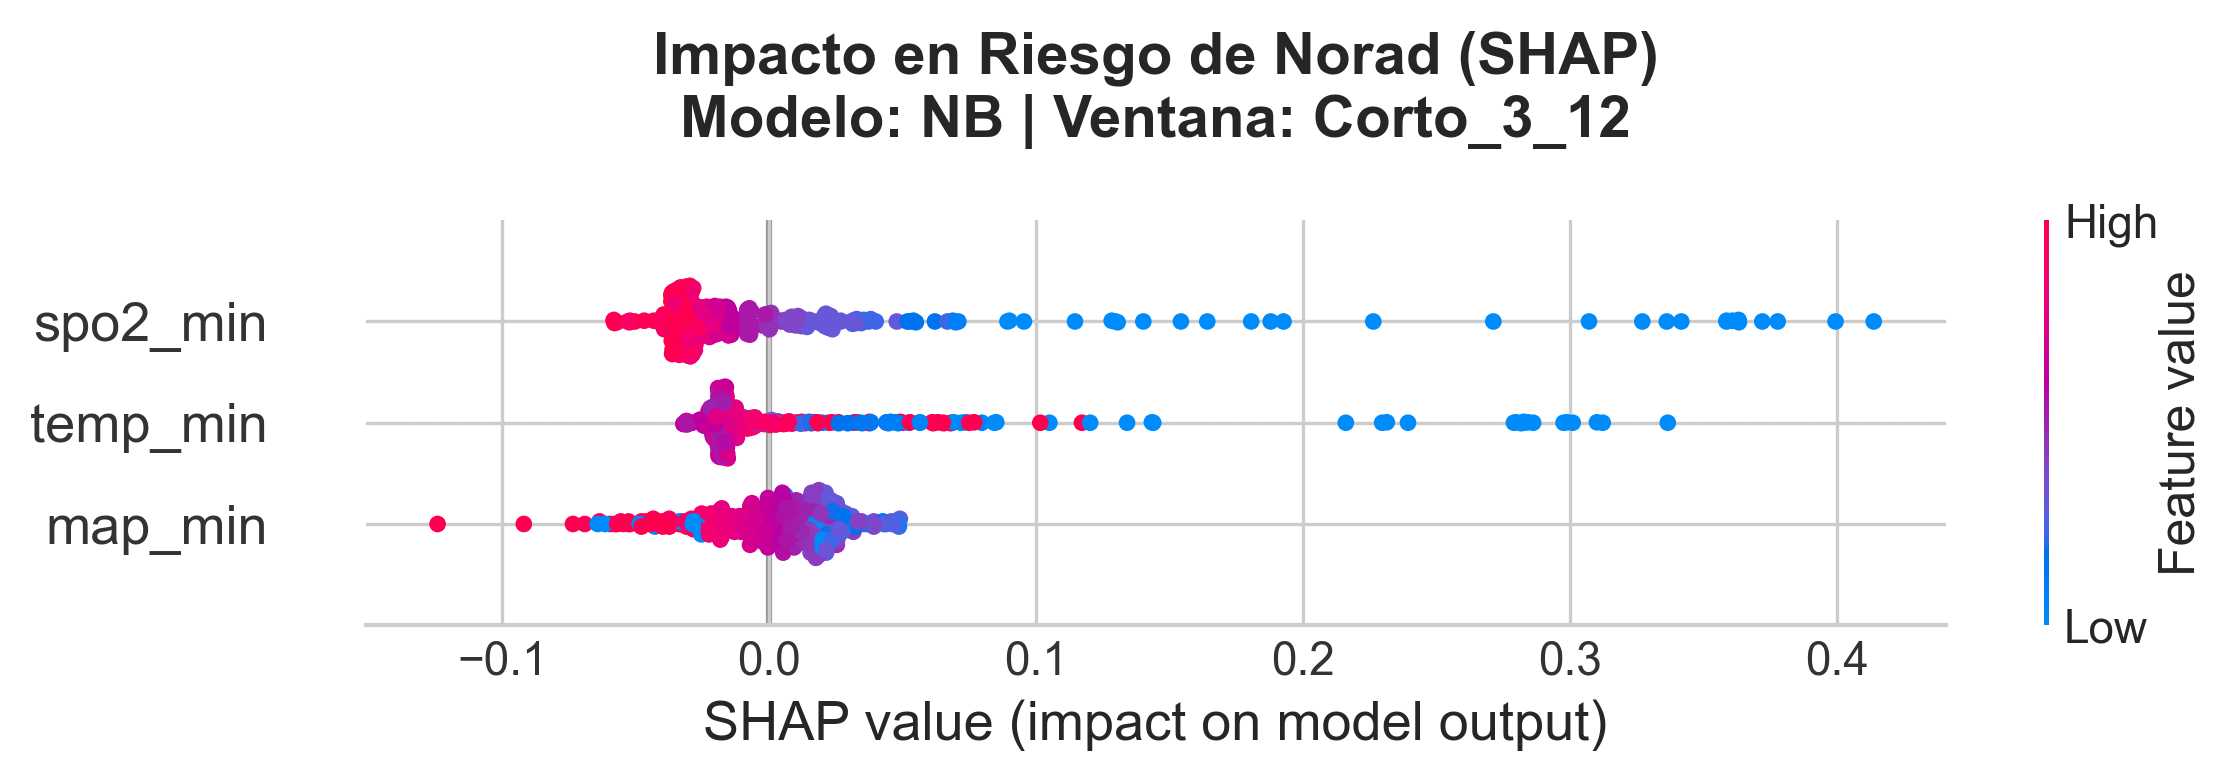
\includegraphics[width=\linewidth]{img/SHAP_Corto_3_12_NB.png}\caption{Naive Bayes}\end{subfigure}
  \caption{Diagramas SHAP de los modelos en la ventana corta (3--12\,h), MIMIC-IV.}
  \label{fig:shap-corto}
\end{figure}
 
\begin{figure}[htbp]
  \centering
  \begin{subfigure}[t]{0.48\textwidth}\centering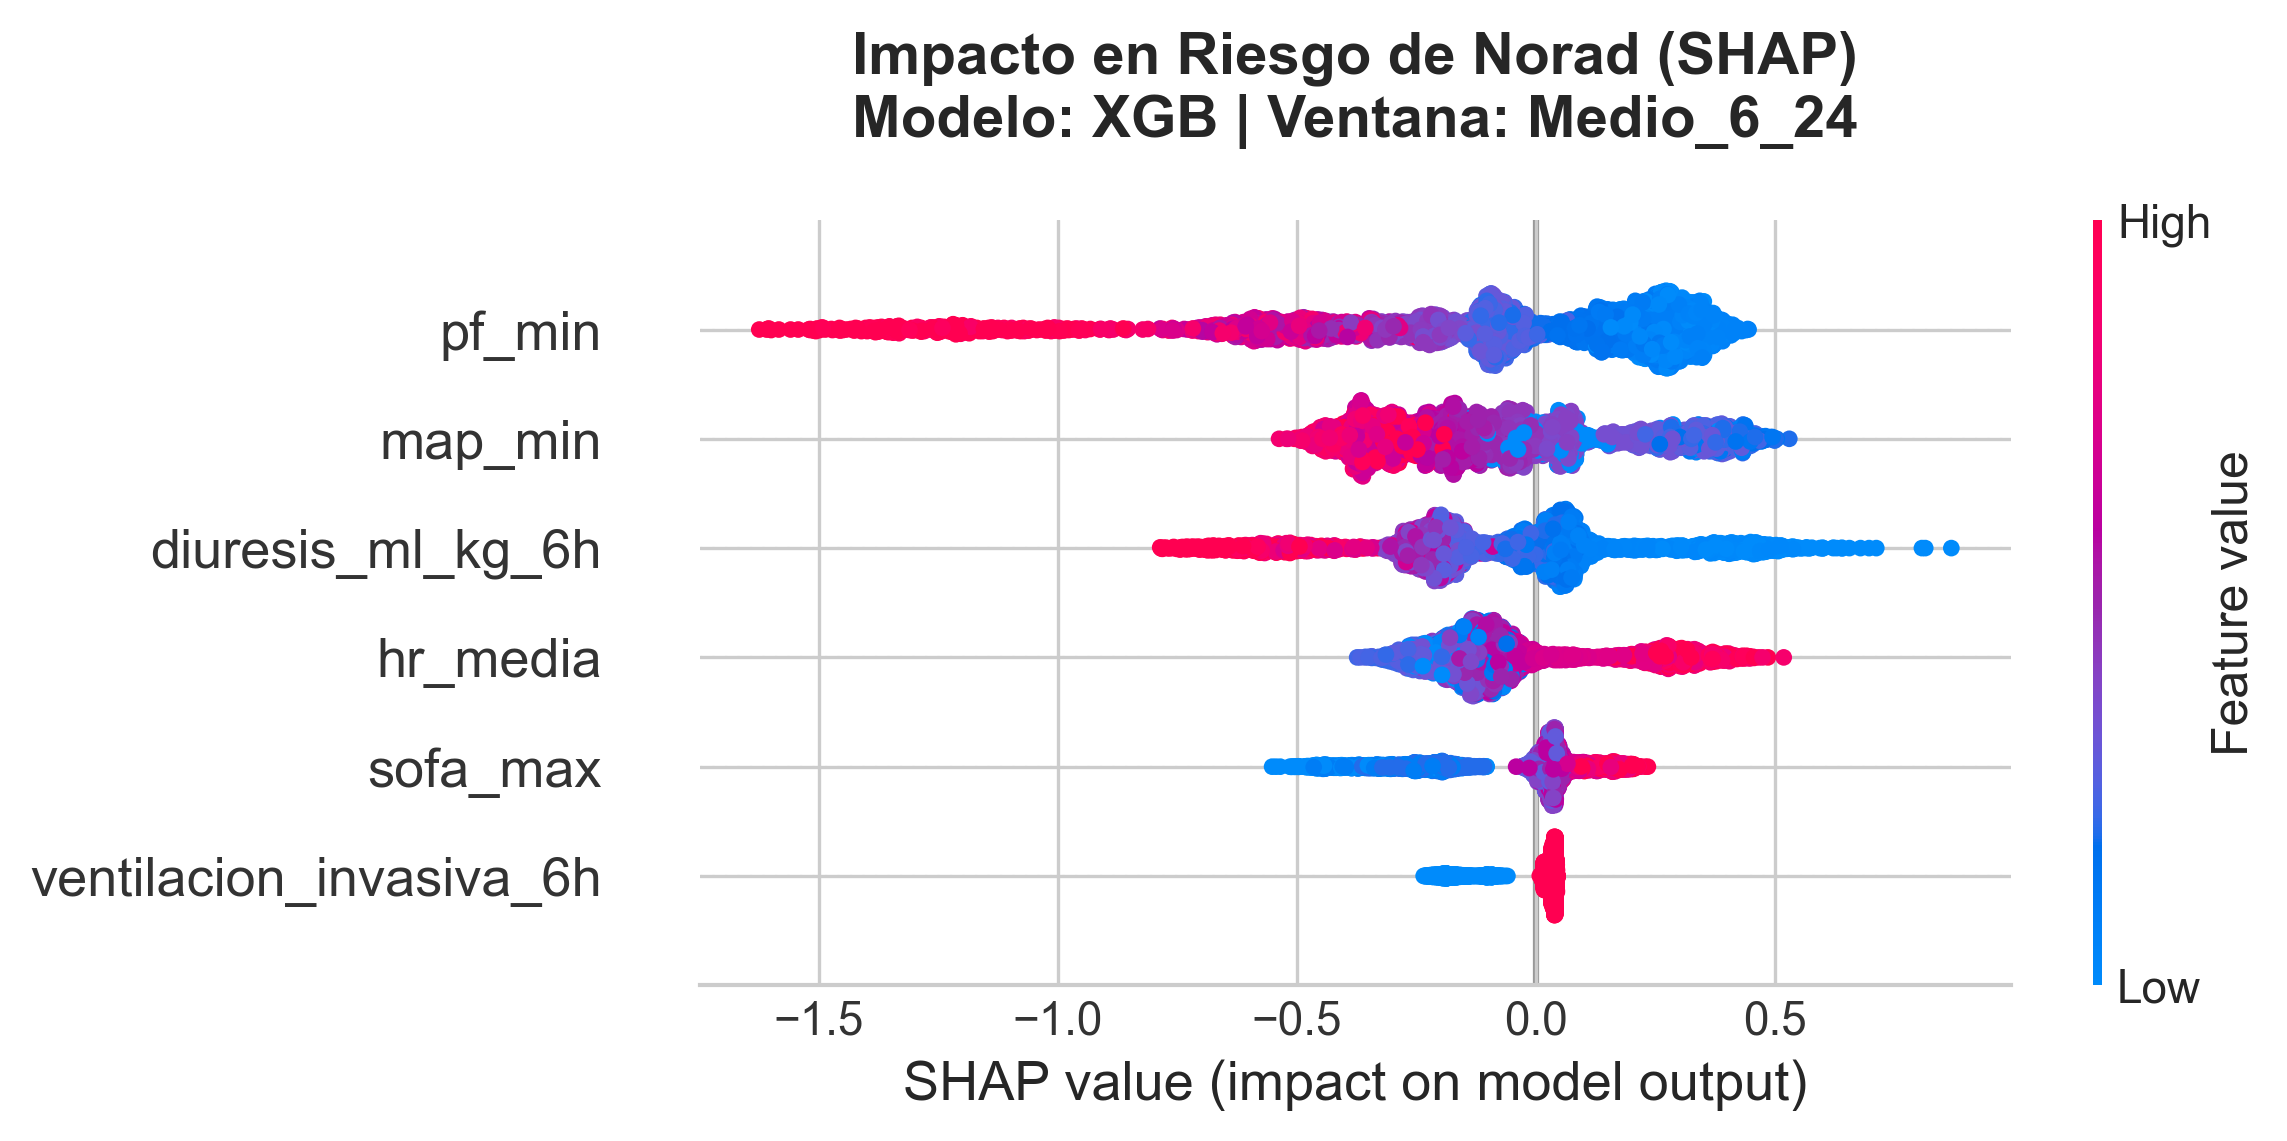
\includegraphics[width=\linewidth]{img/SHAP_Medio_6_24_XGB.png}\caption{XGBoost}\end{subfigure}\hfill
  \begin{subfigure}[t]{0.48\textwidth}\centering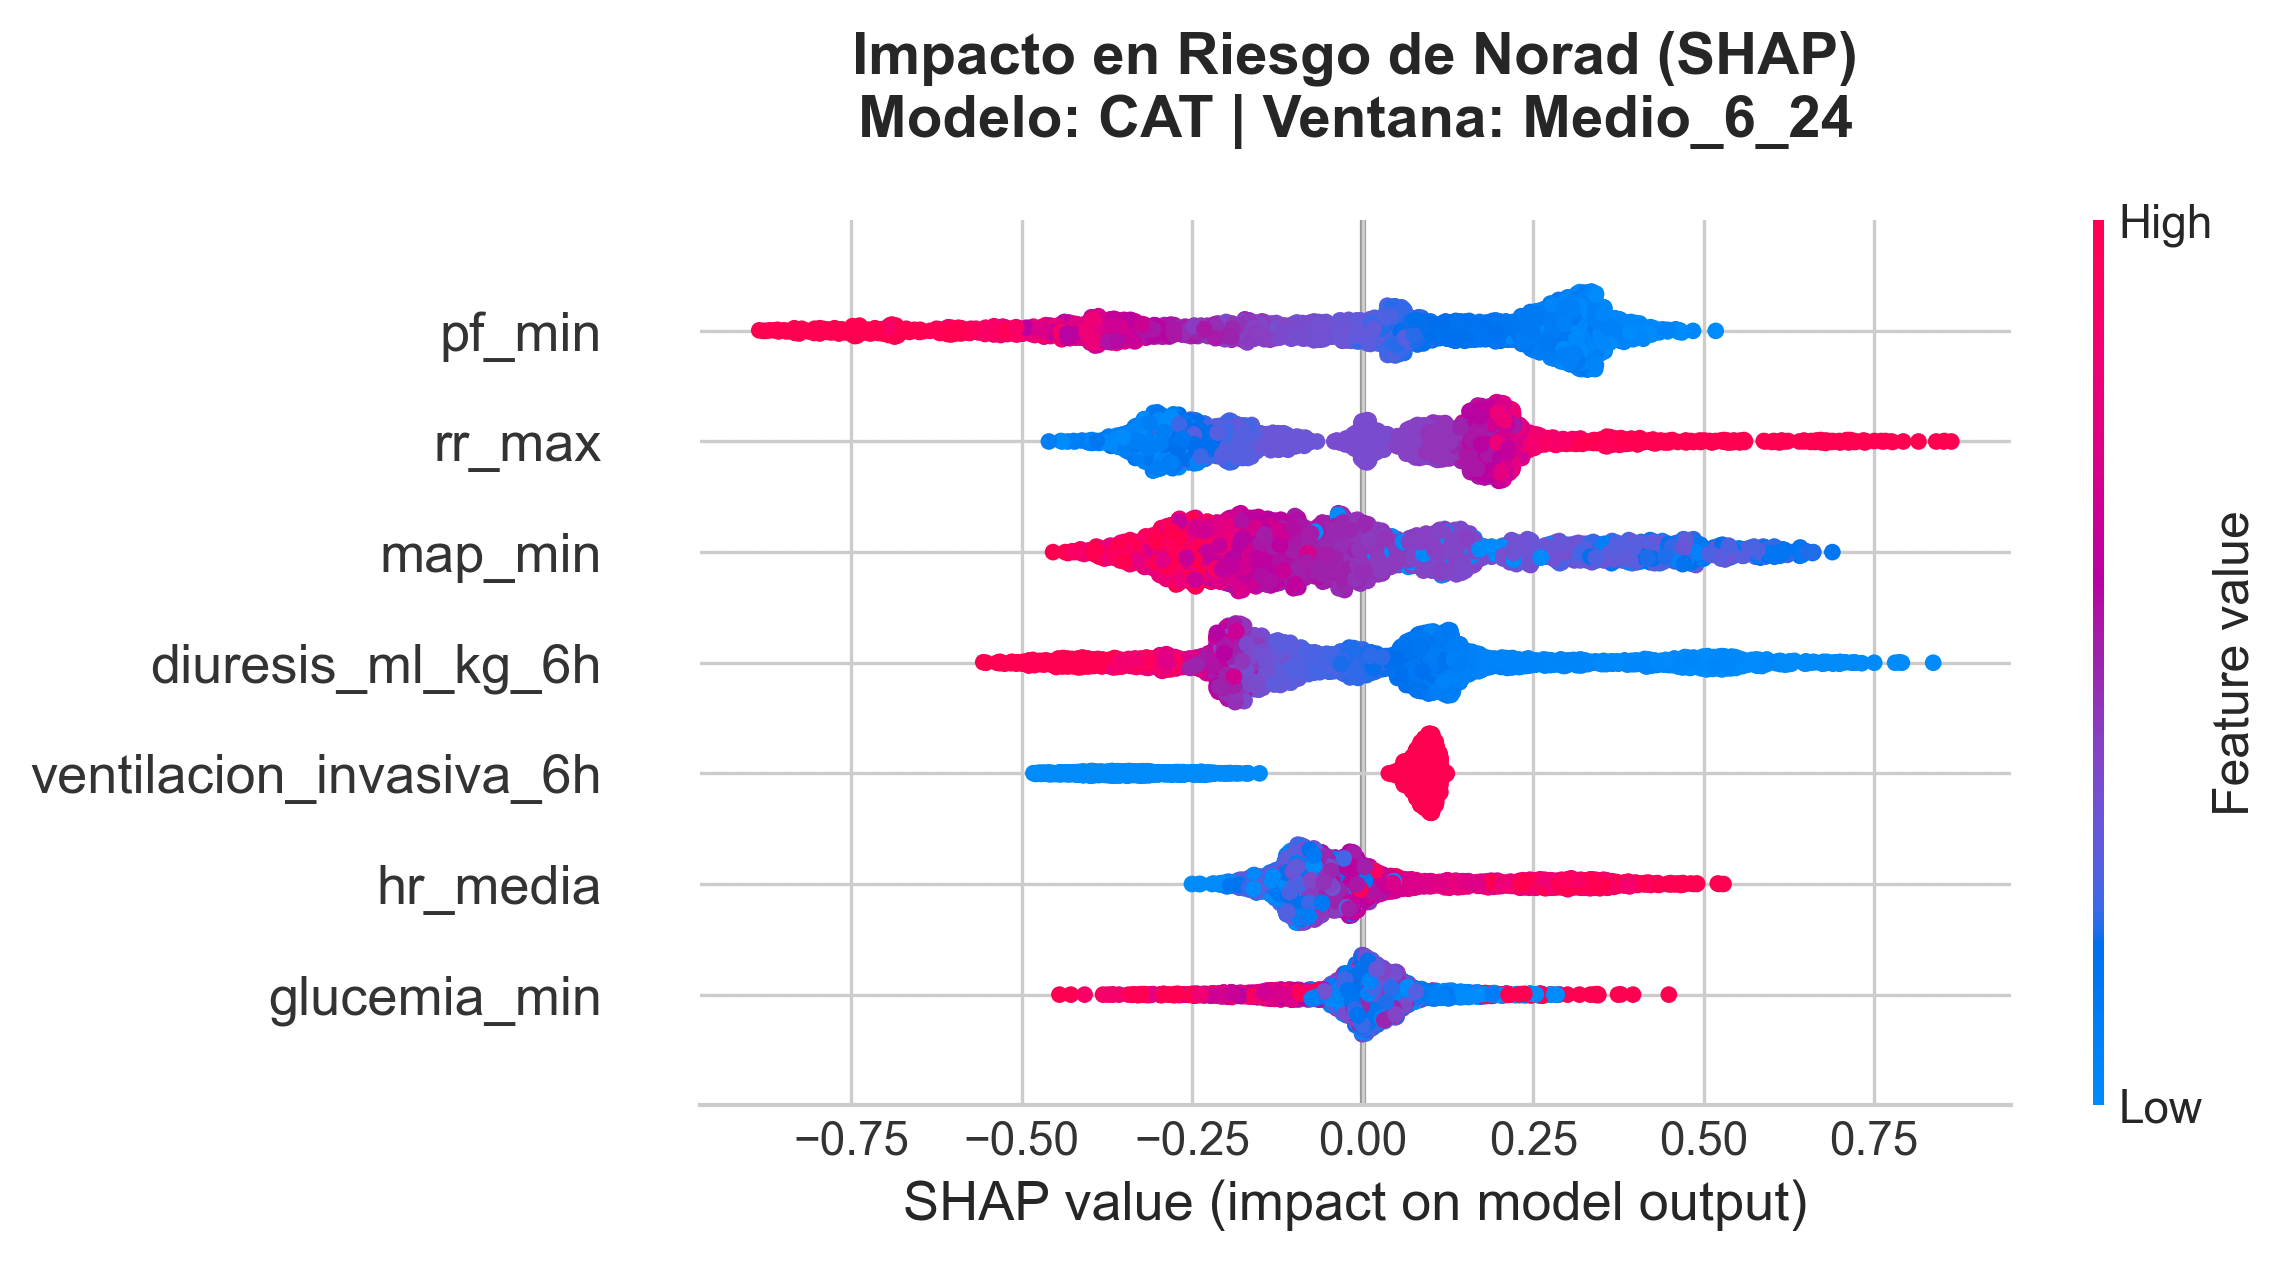
\includegraphics[width=\linewidth]{img/SHAP_Medio_6_24_CAT.png}\caption{CatBoost}\end{subfigure}\\[6pt]
  \begin{subfigure}[t]{0.48\textwidth}\centering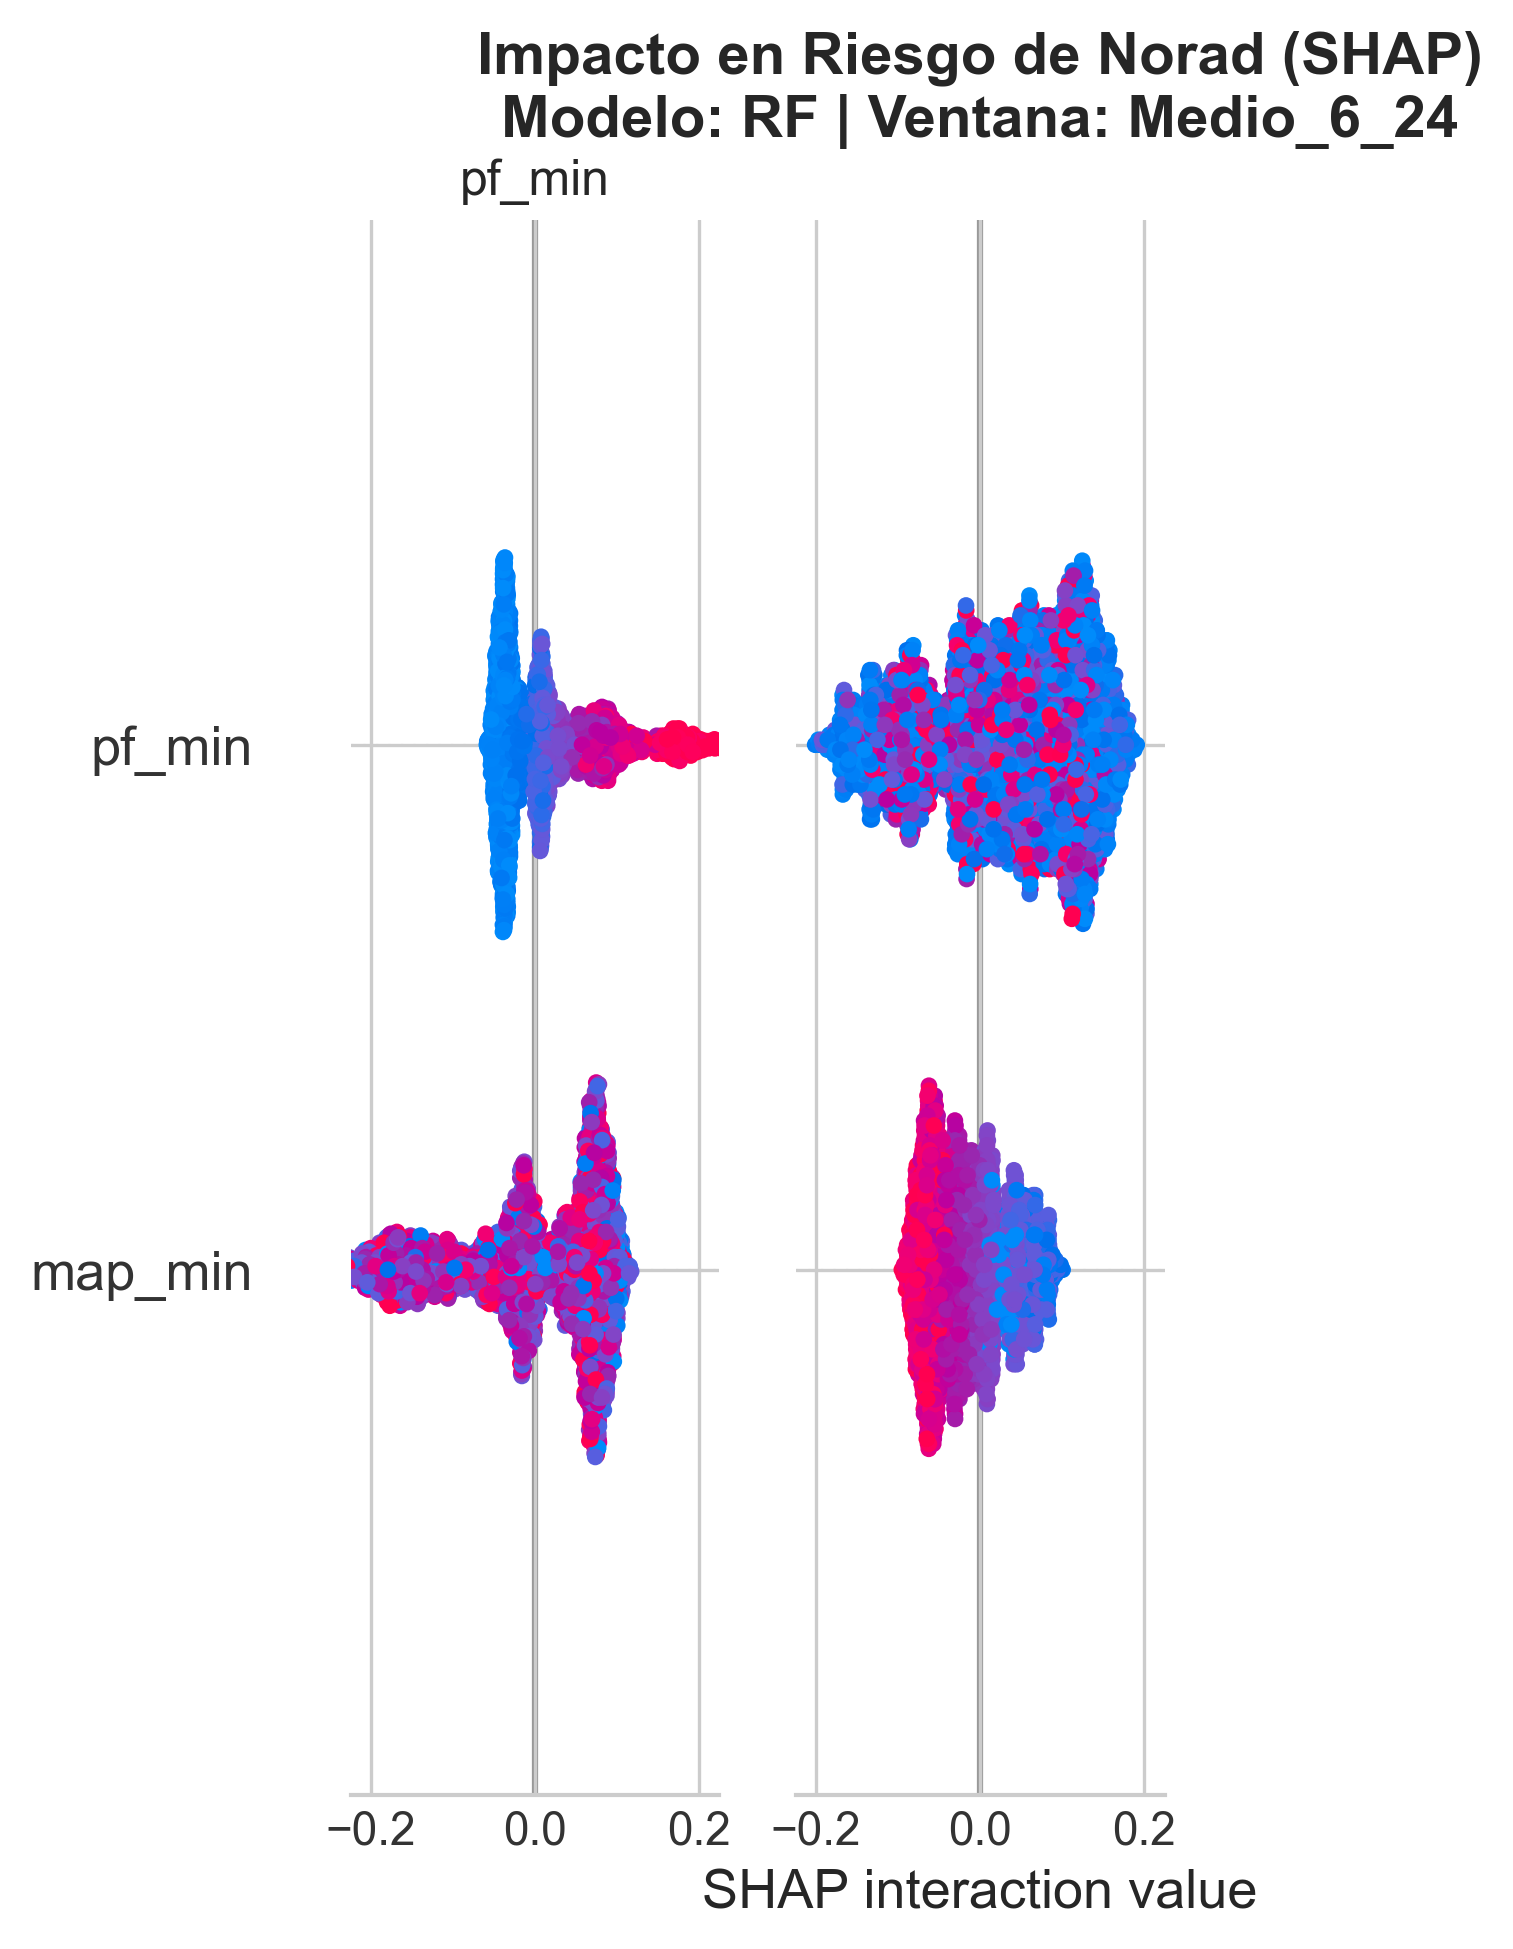
\includegraphics[width=\linewidth]{img/SHAP_Medio_6_24_RF.png}\caption{Random Forest}\end{subfigure}\hfill
  \begin{subfigure}[t]{0.48\textwidth}\centering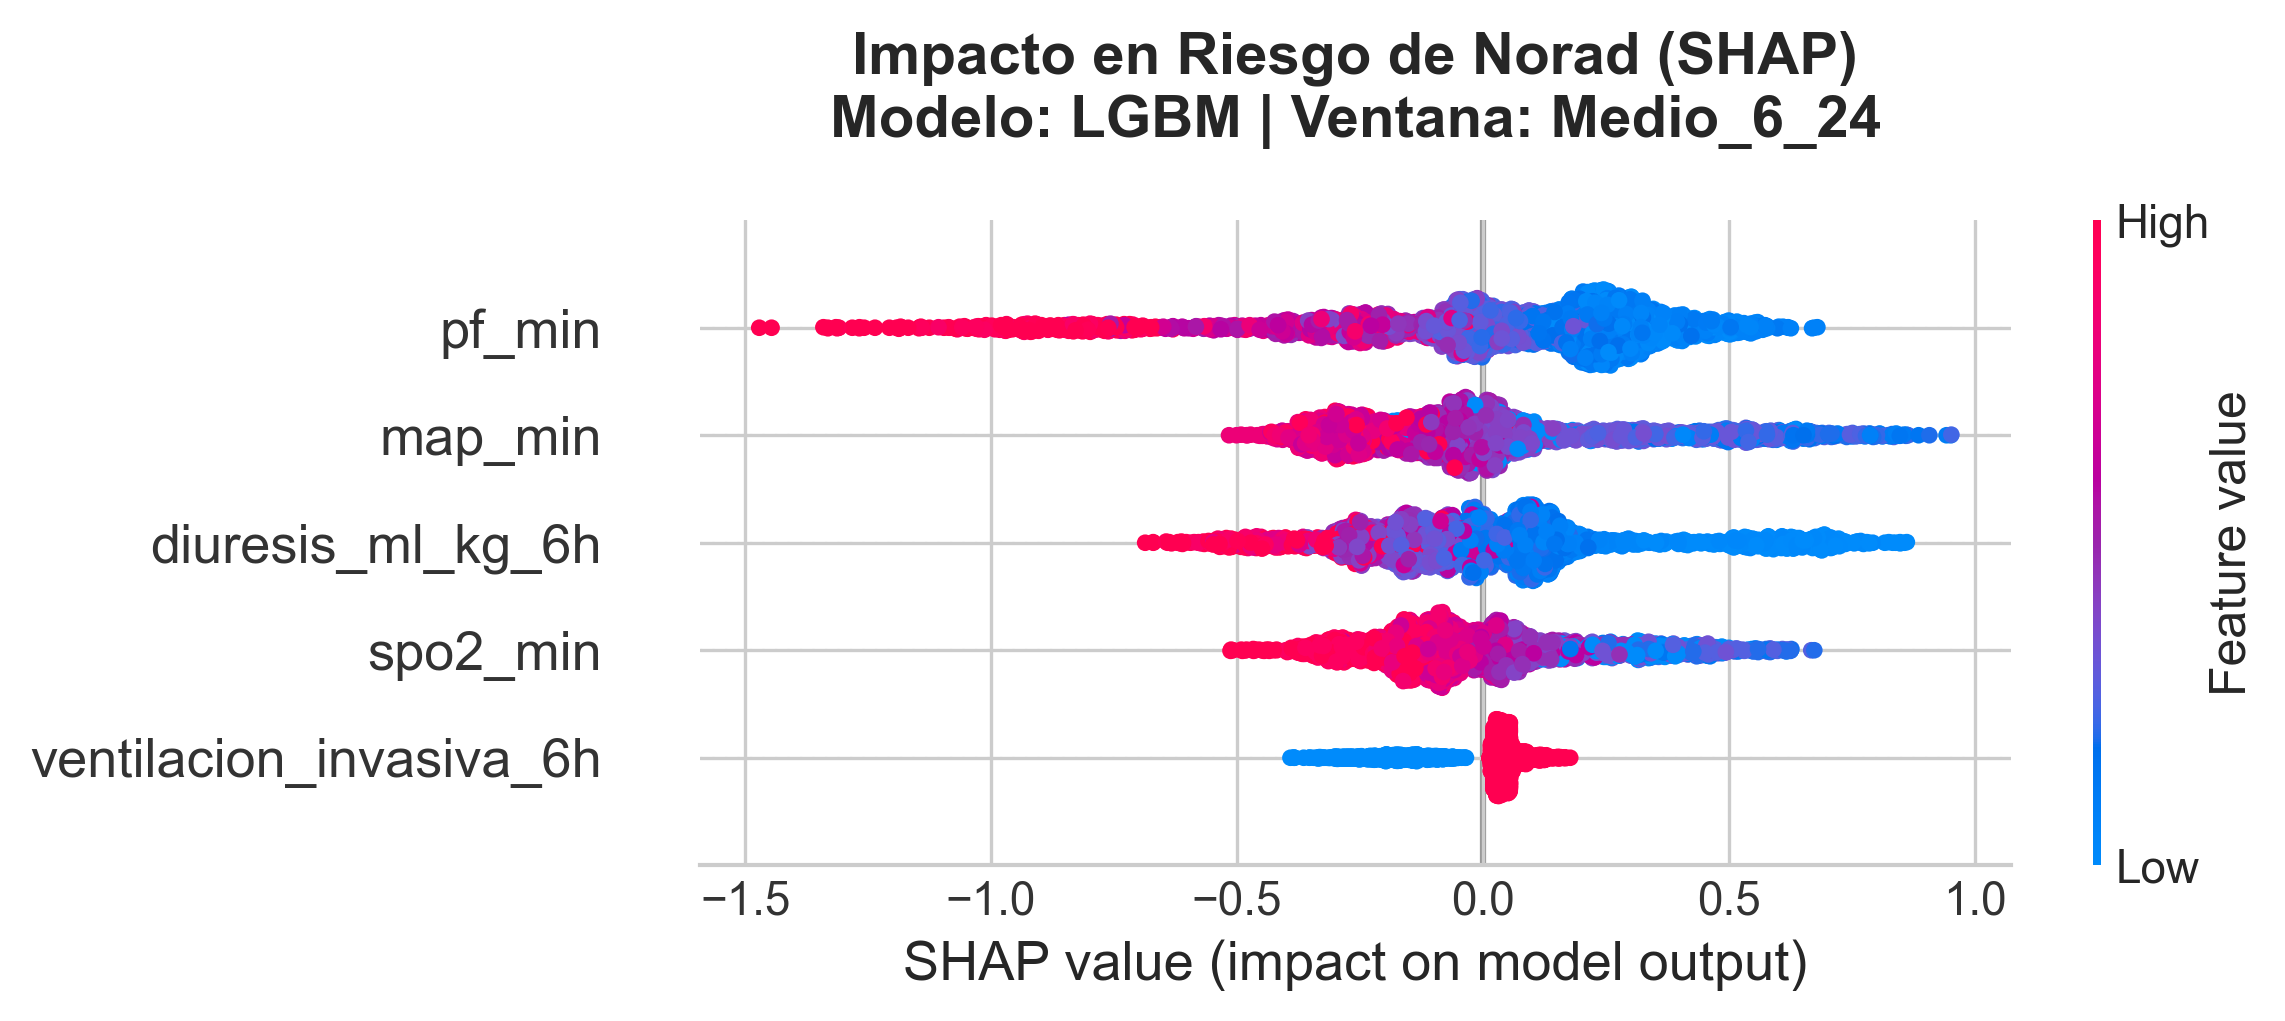
\includegraphics[width=\linewidth]{img/SHAP_Medio_6_24_LGBM.png}\caption{LightGBM}\end{subfigure}\\[6pt]
  \begin{subfigure}[t]{0.48\textwidth}\centering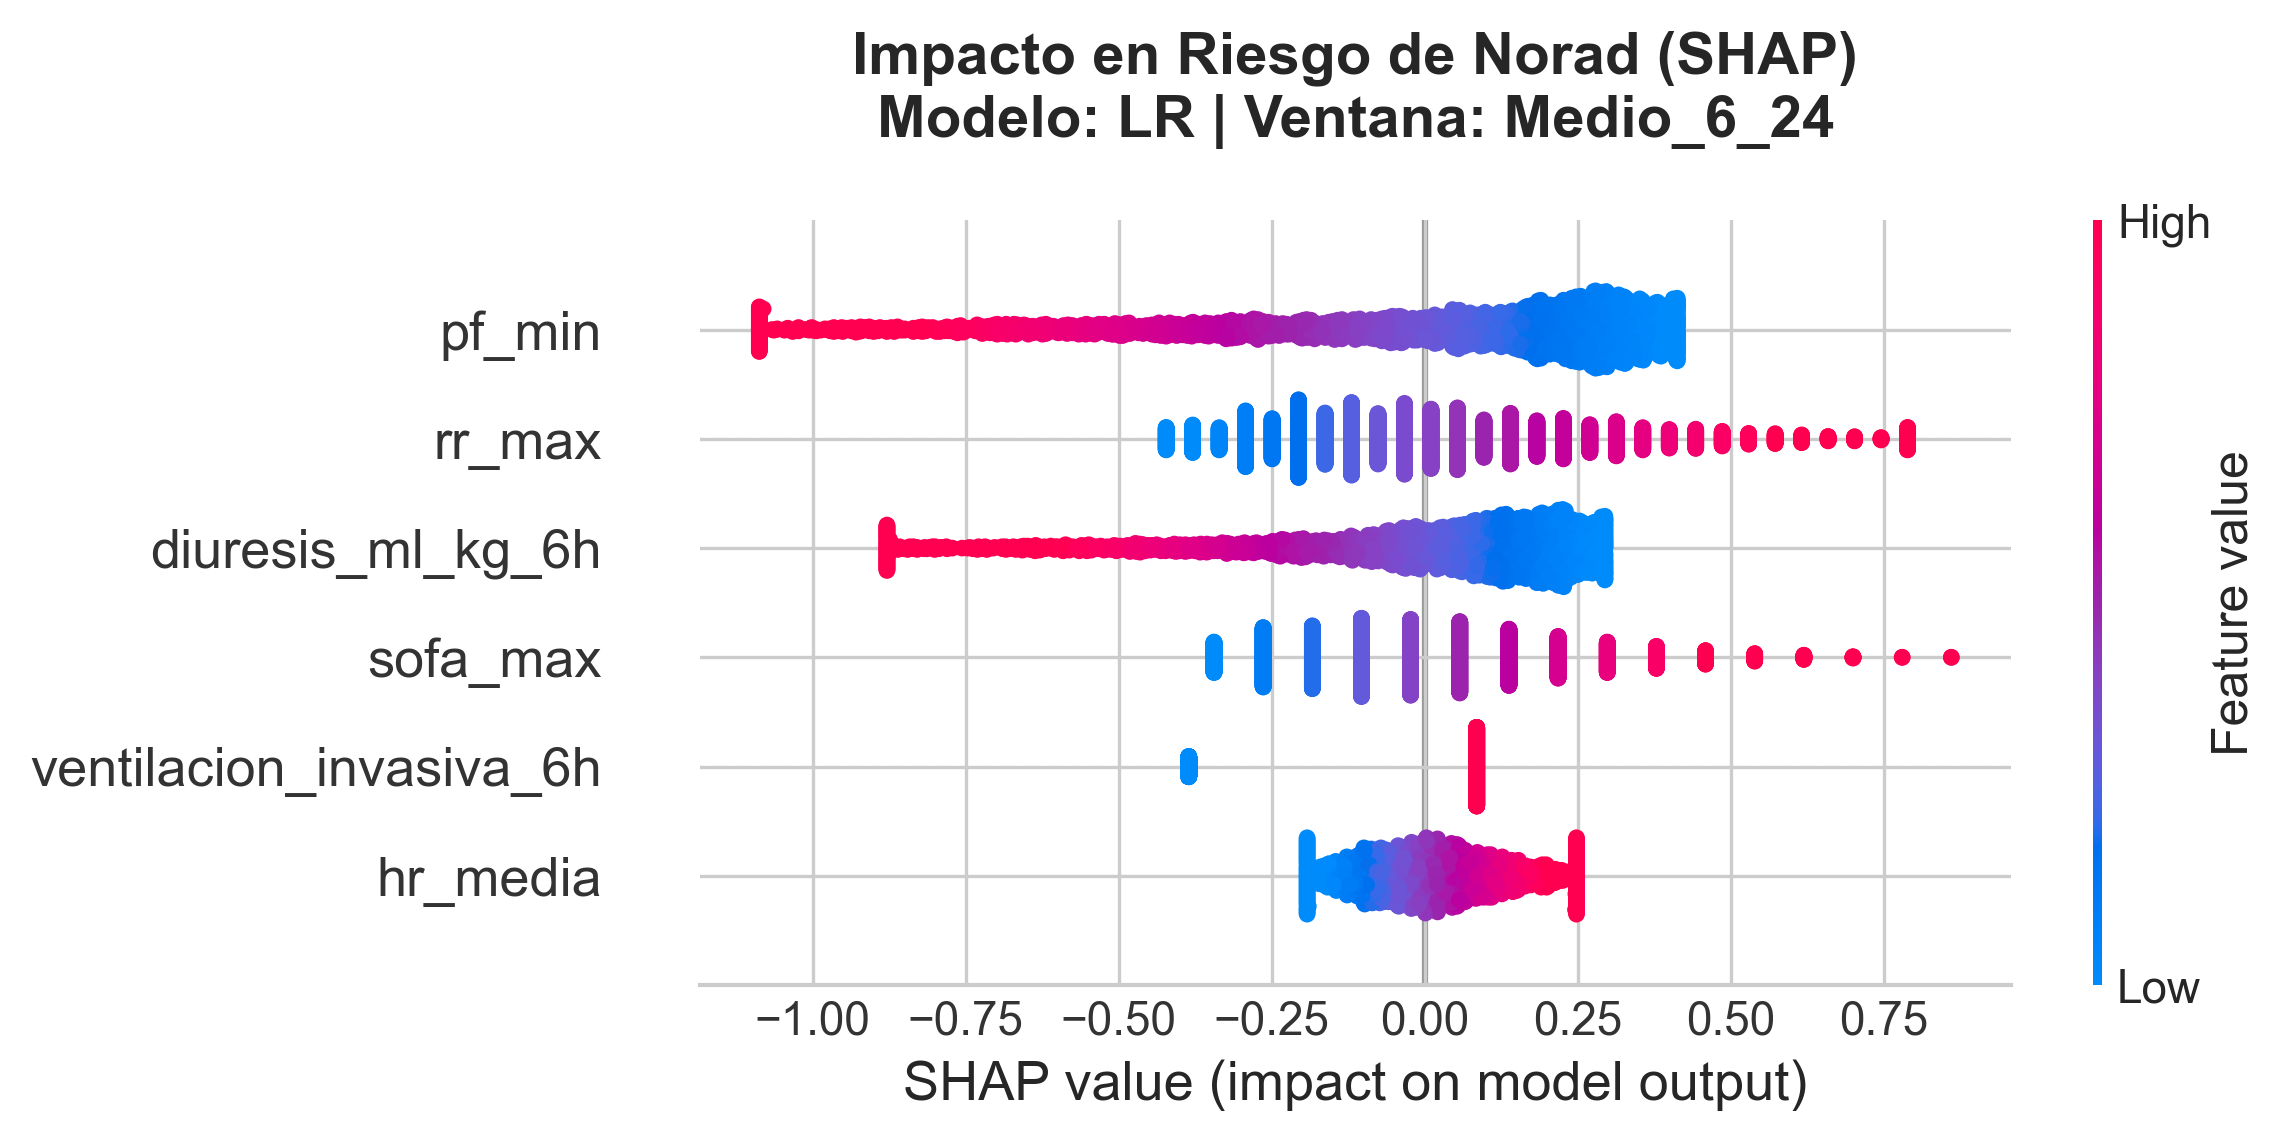
\includegraphics[width=\linewidth]{img/SHAP_Medio_6_24_LR.png}\caption{Regresión logística}\end{subfigure}\hfill
  \begin{subfigure}[t]{0.48\textwidth}\centering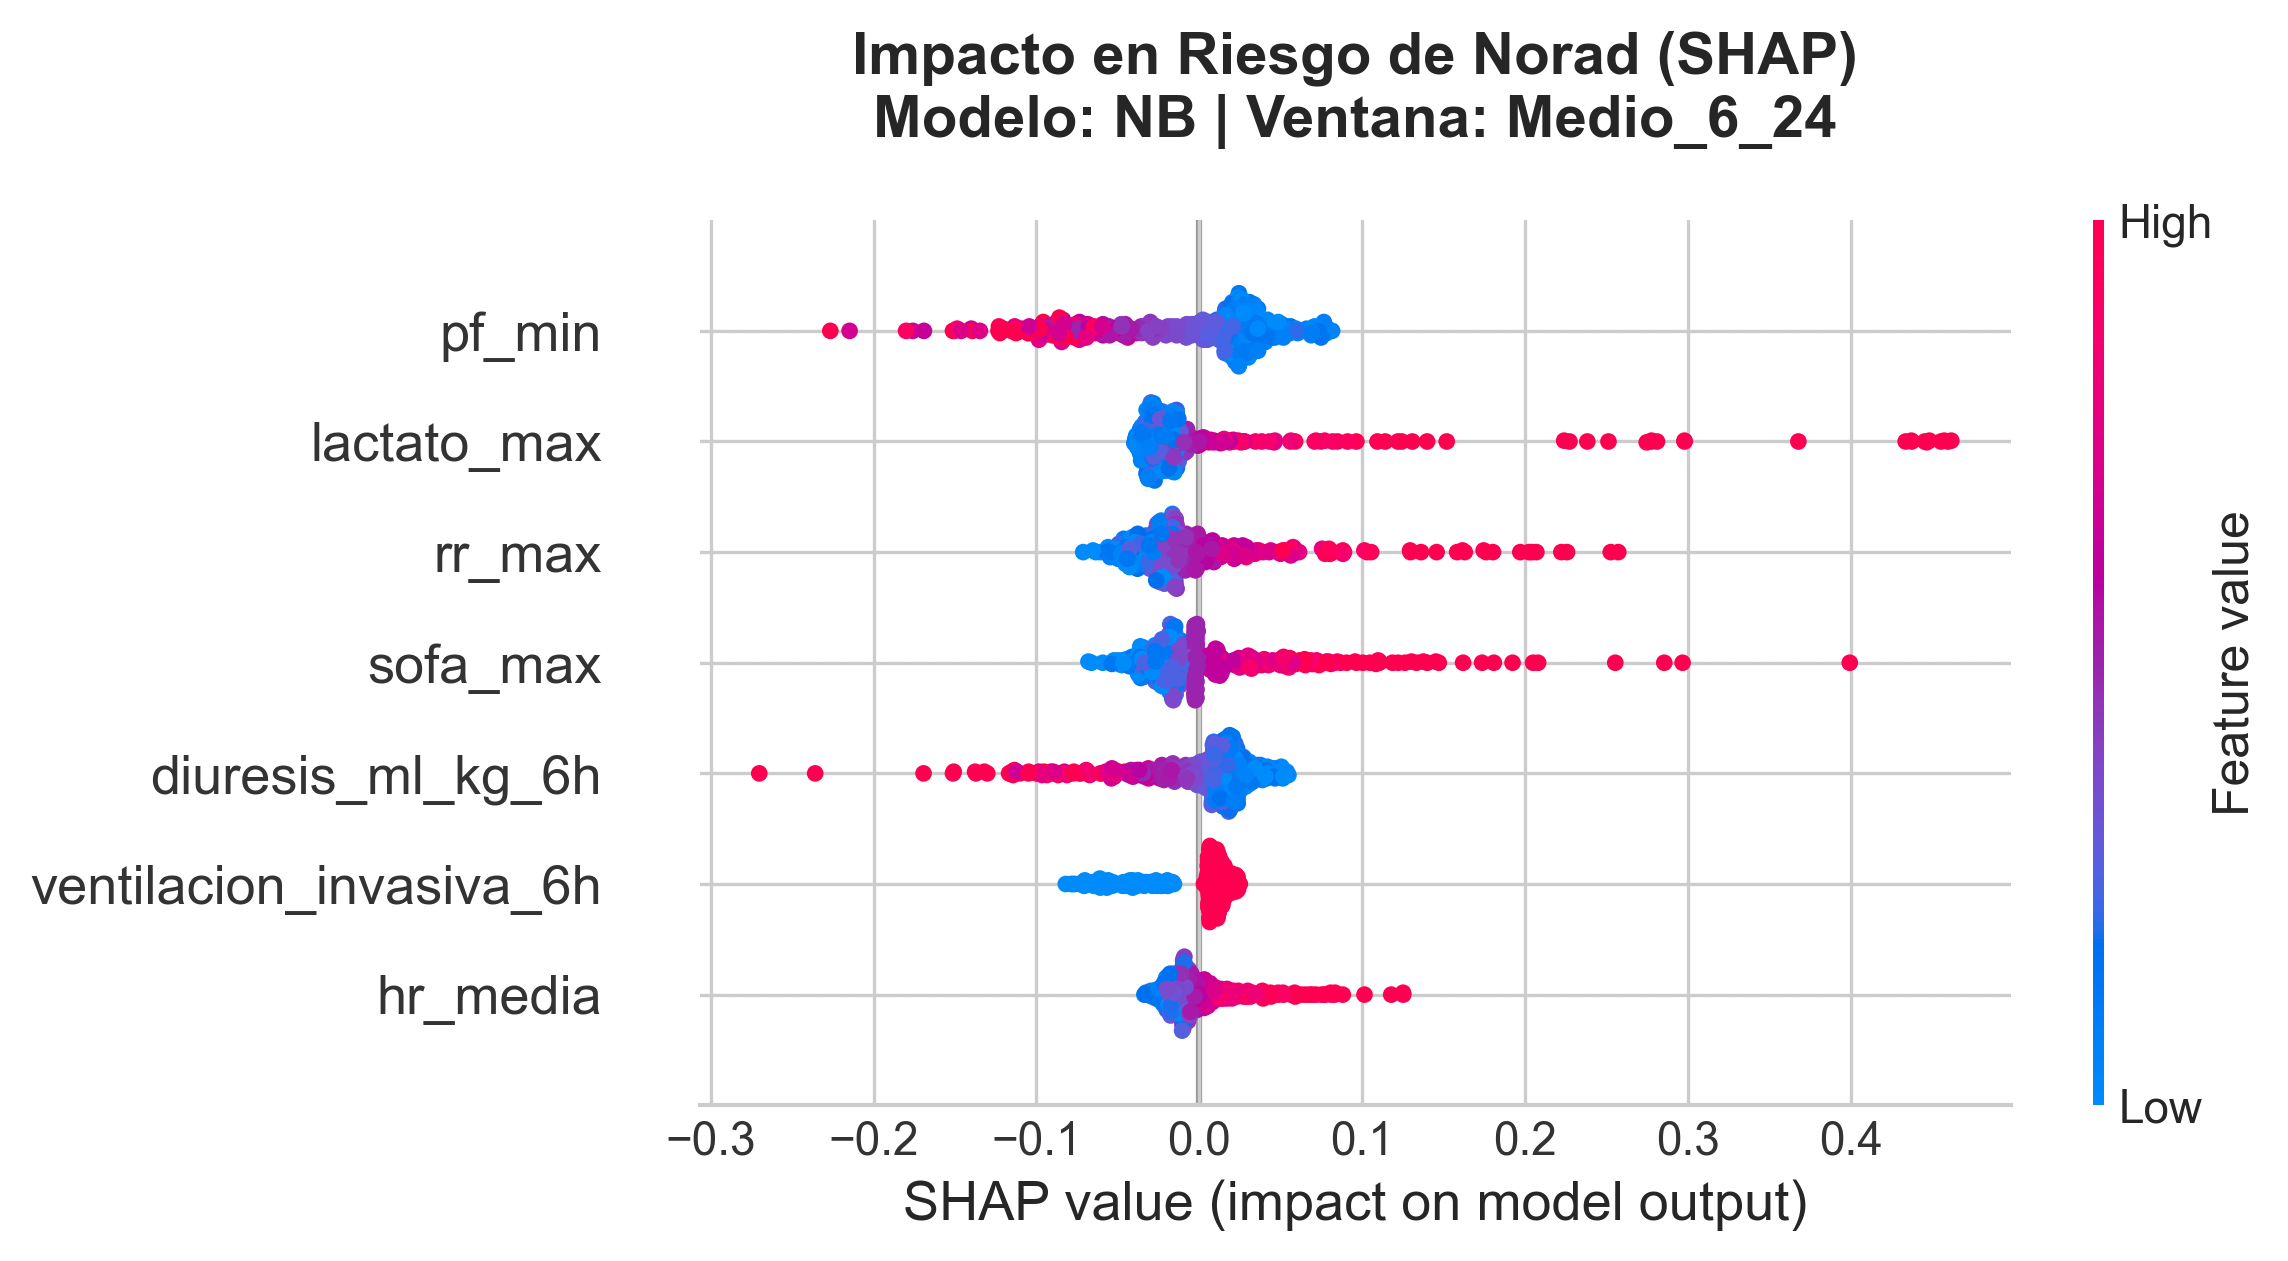
\includegraphics[width=\linewidth]{img/SHAP_Medio_6_24_NB.png}\caption{Naive Bayes}\end{subfigure}
  \caption{Diagramas SHAP de los modelos en la ventana media (6--24\,h), MIMIC-IV.
  En CatBoost la dirección del efecto de la diuresis resultó clínicamente
  incoherente, lo que motivó priorizar XGBoost calibrado.}
  \label{fig:shap-medio}
\end{figure}
 
\begin{figure}[htbp]
  \centering
  \begin{subfigure}[t]{0.48\textwidth}\centering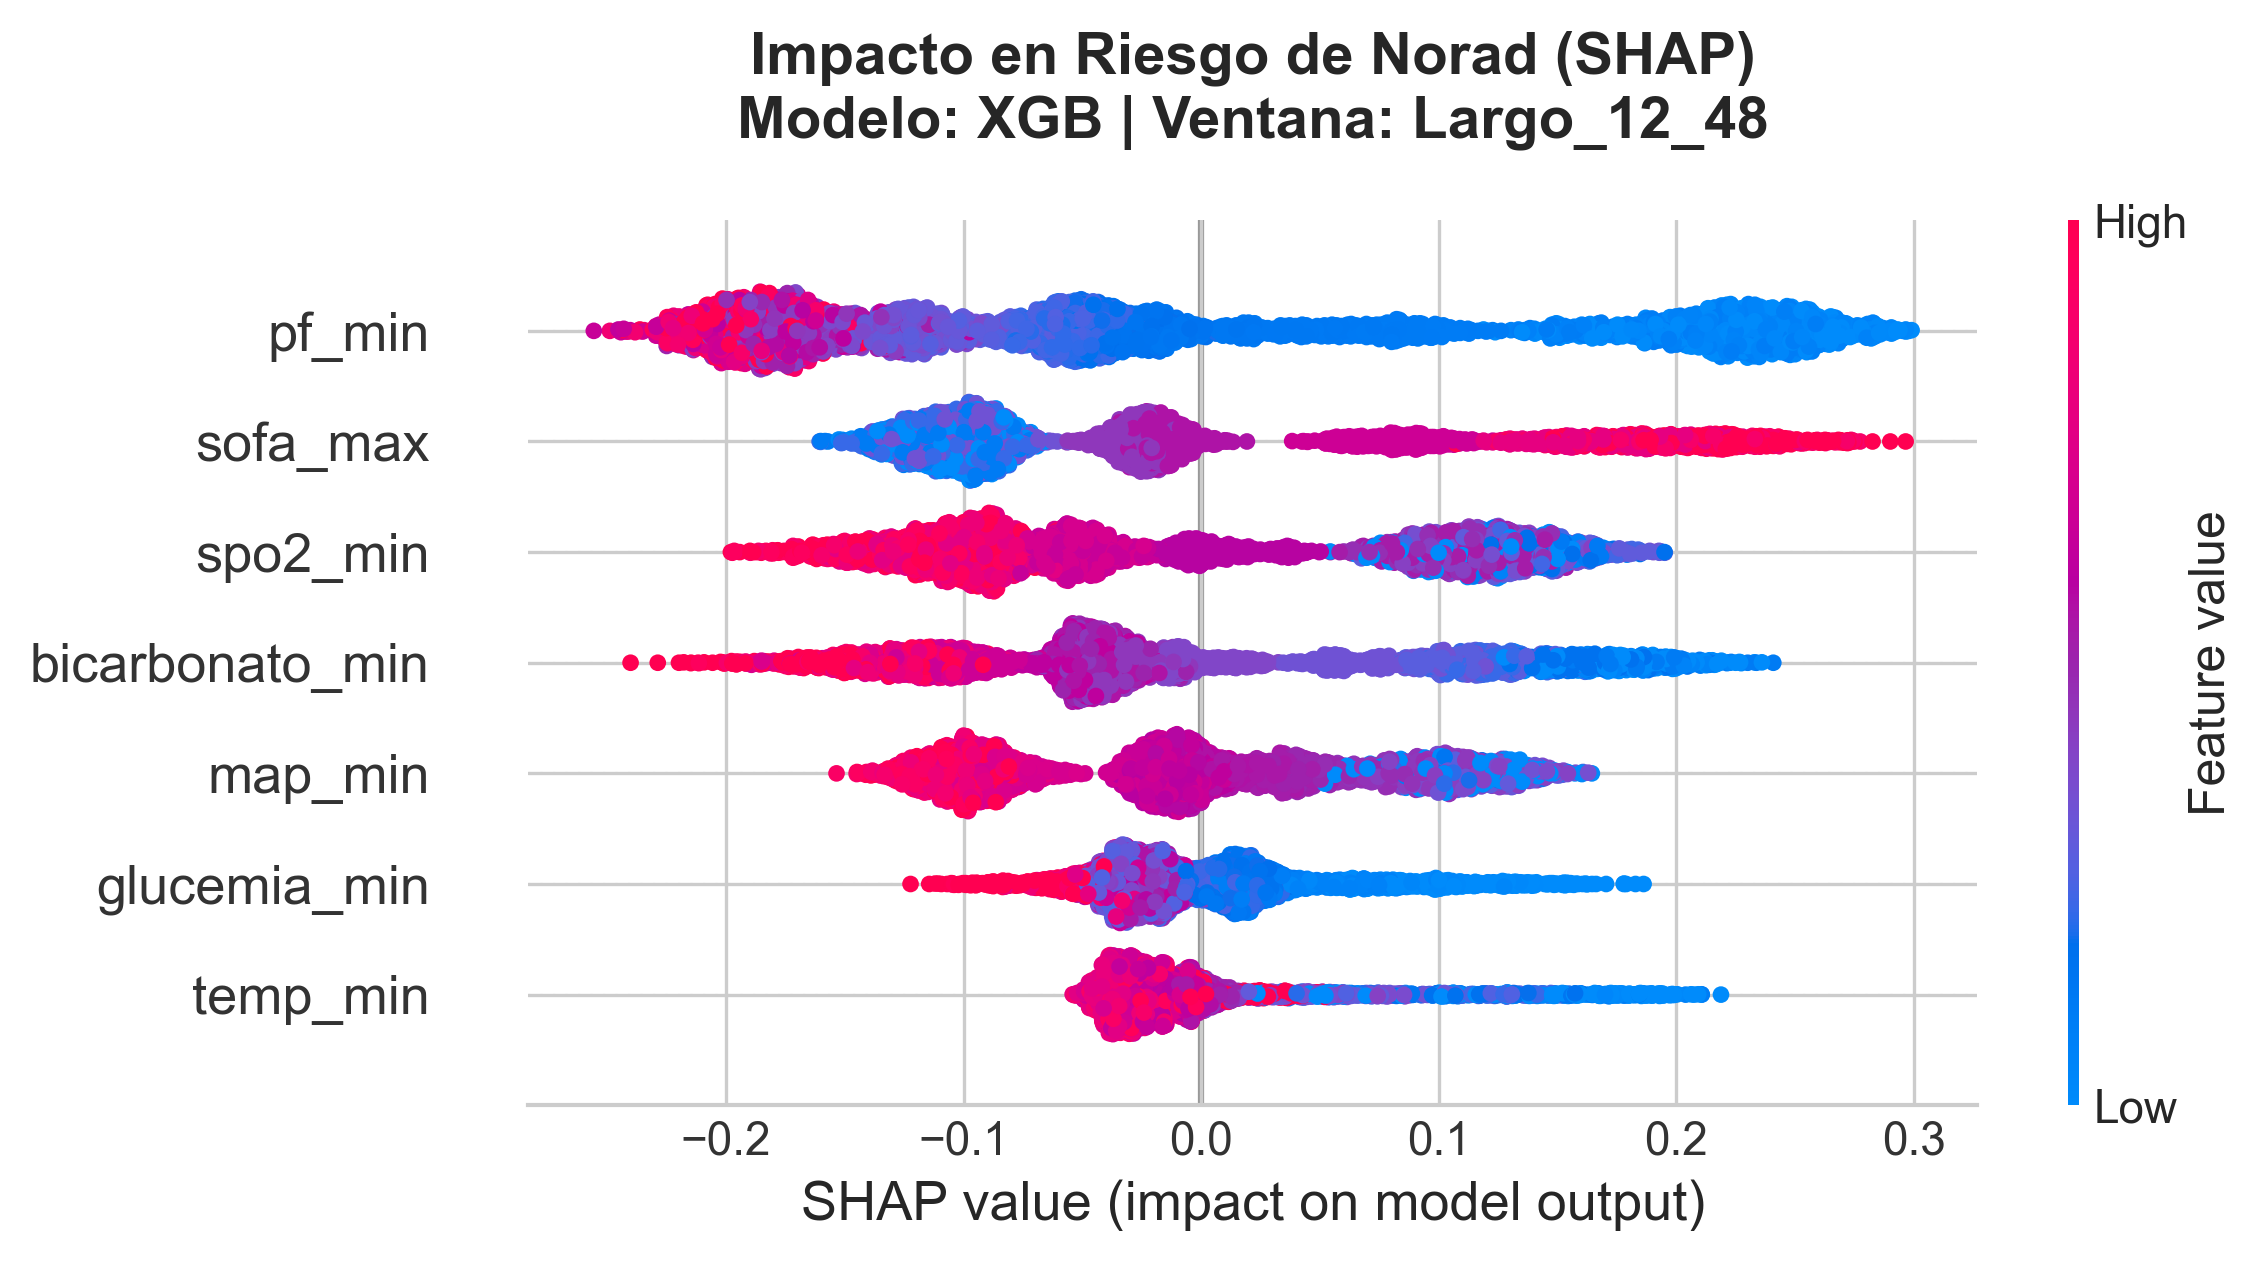
\includegraphics[width=\linewidth]{img/SHAP_Largo_12_48_XGB.png}\caption{XGBoost}\end{subfigure}\hfill
  \begin{subfigure}[t]{0.48\textwidth}\centering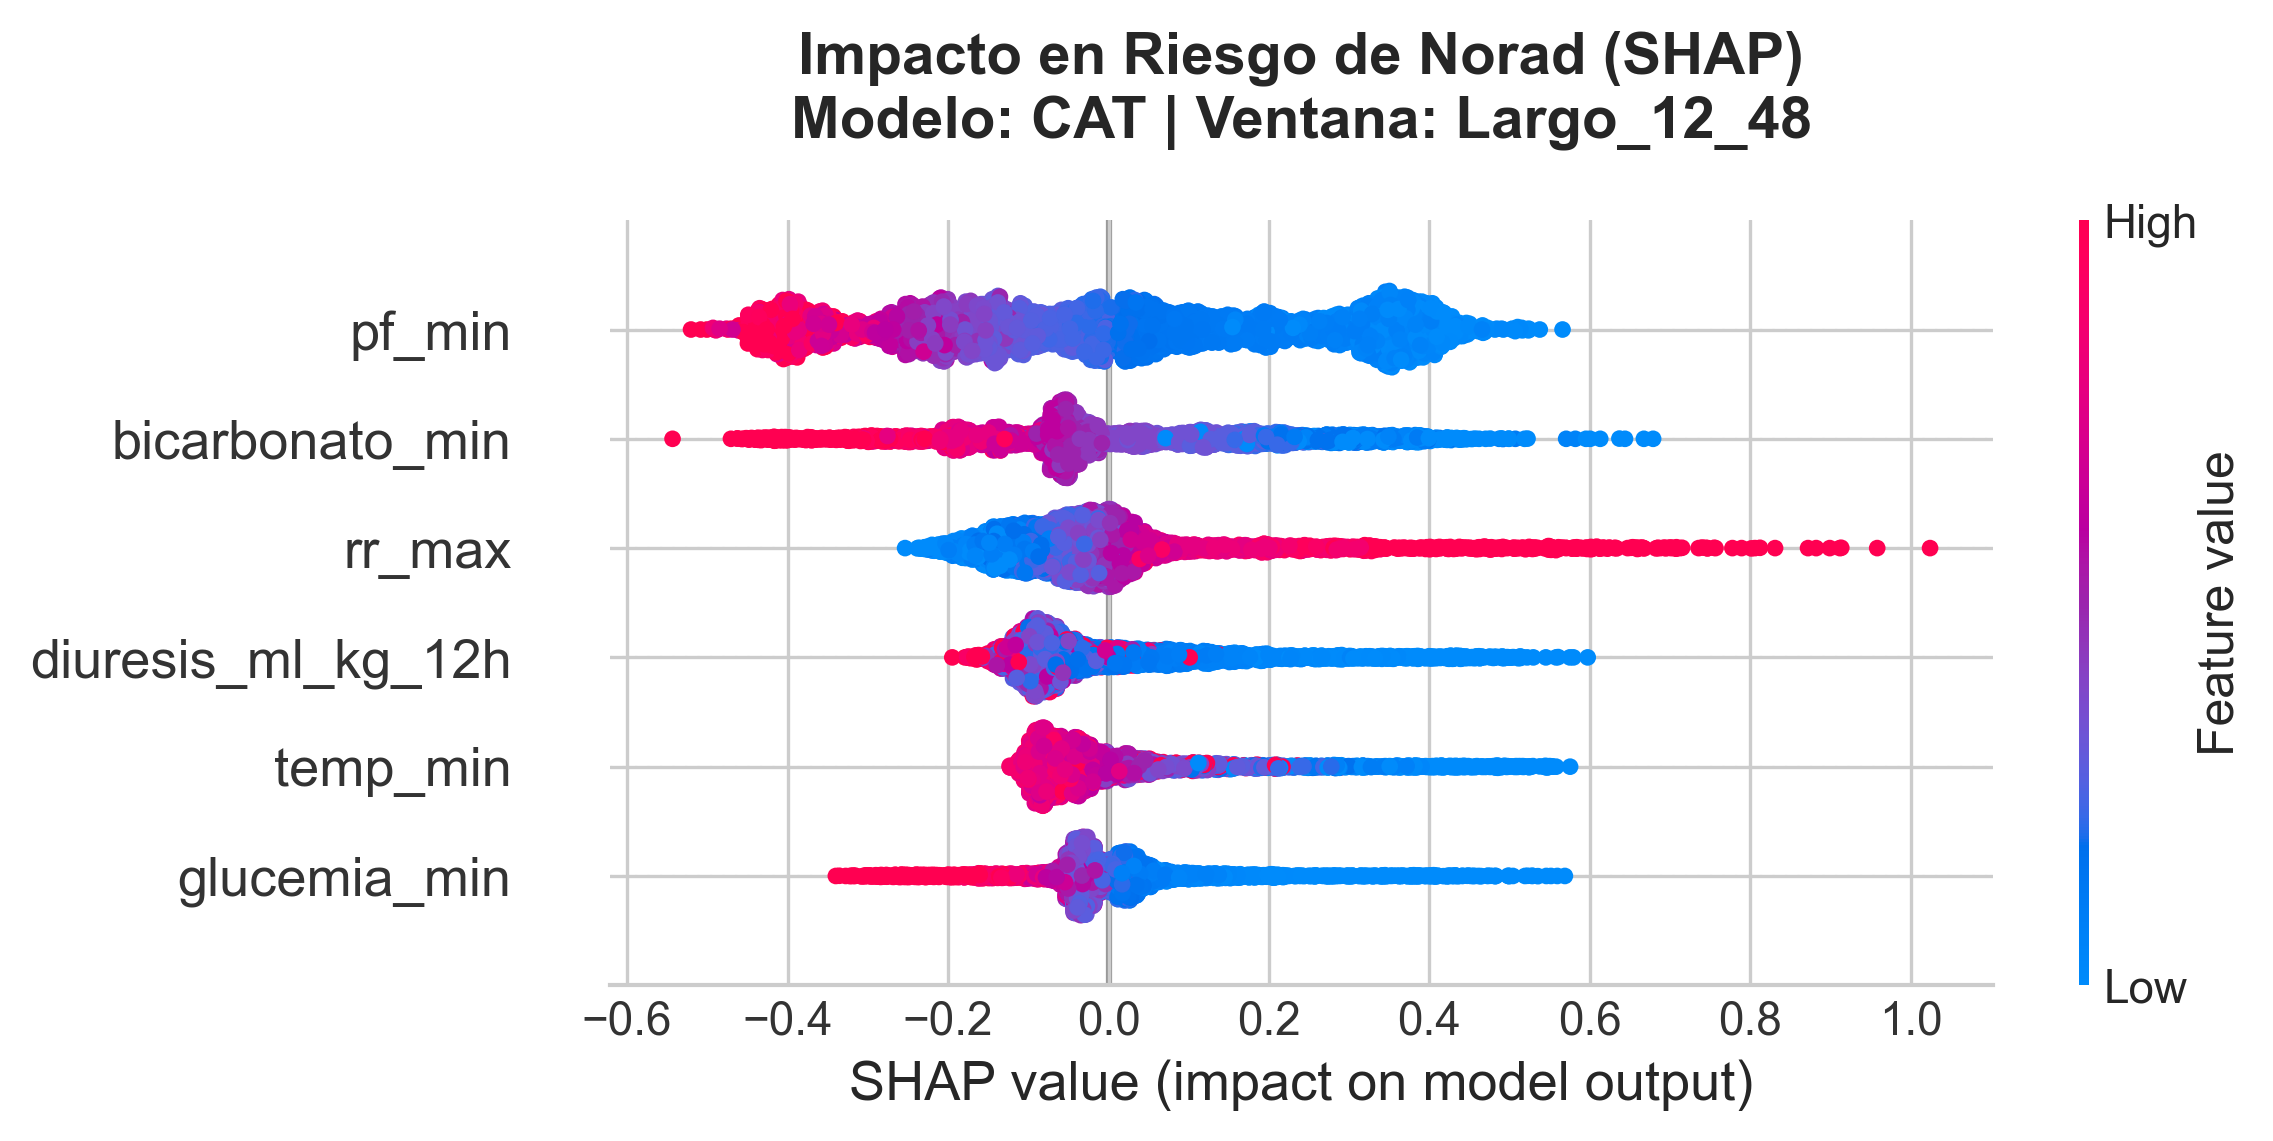
\includegraphics[width=\linewidth]{img/SHAP_Largo_12_48_CAT.png}\caption{CatBoost}\end{subfigure}\\[6pt]
  \begin{subfigure}[t]{0.48\textwidth}\centering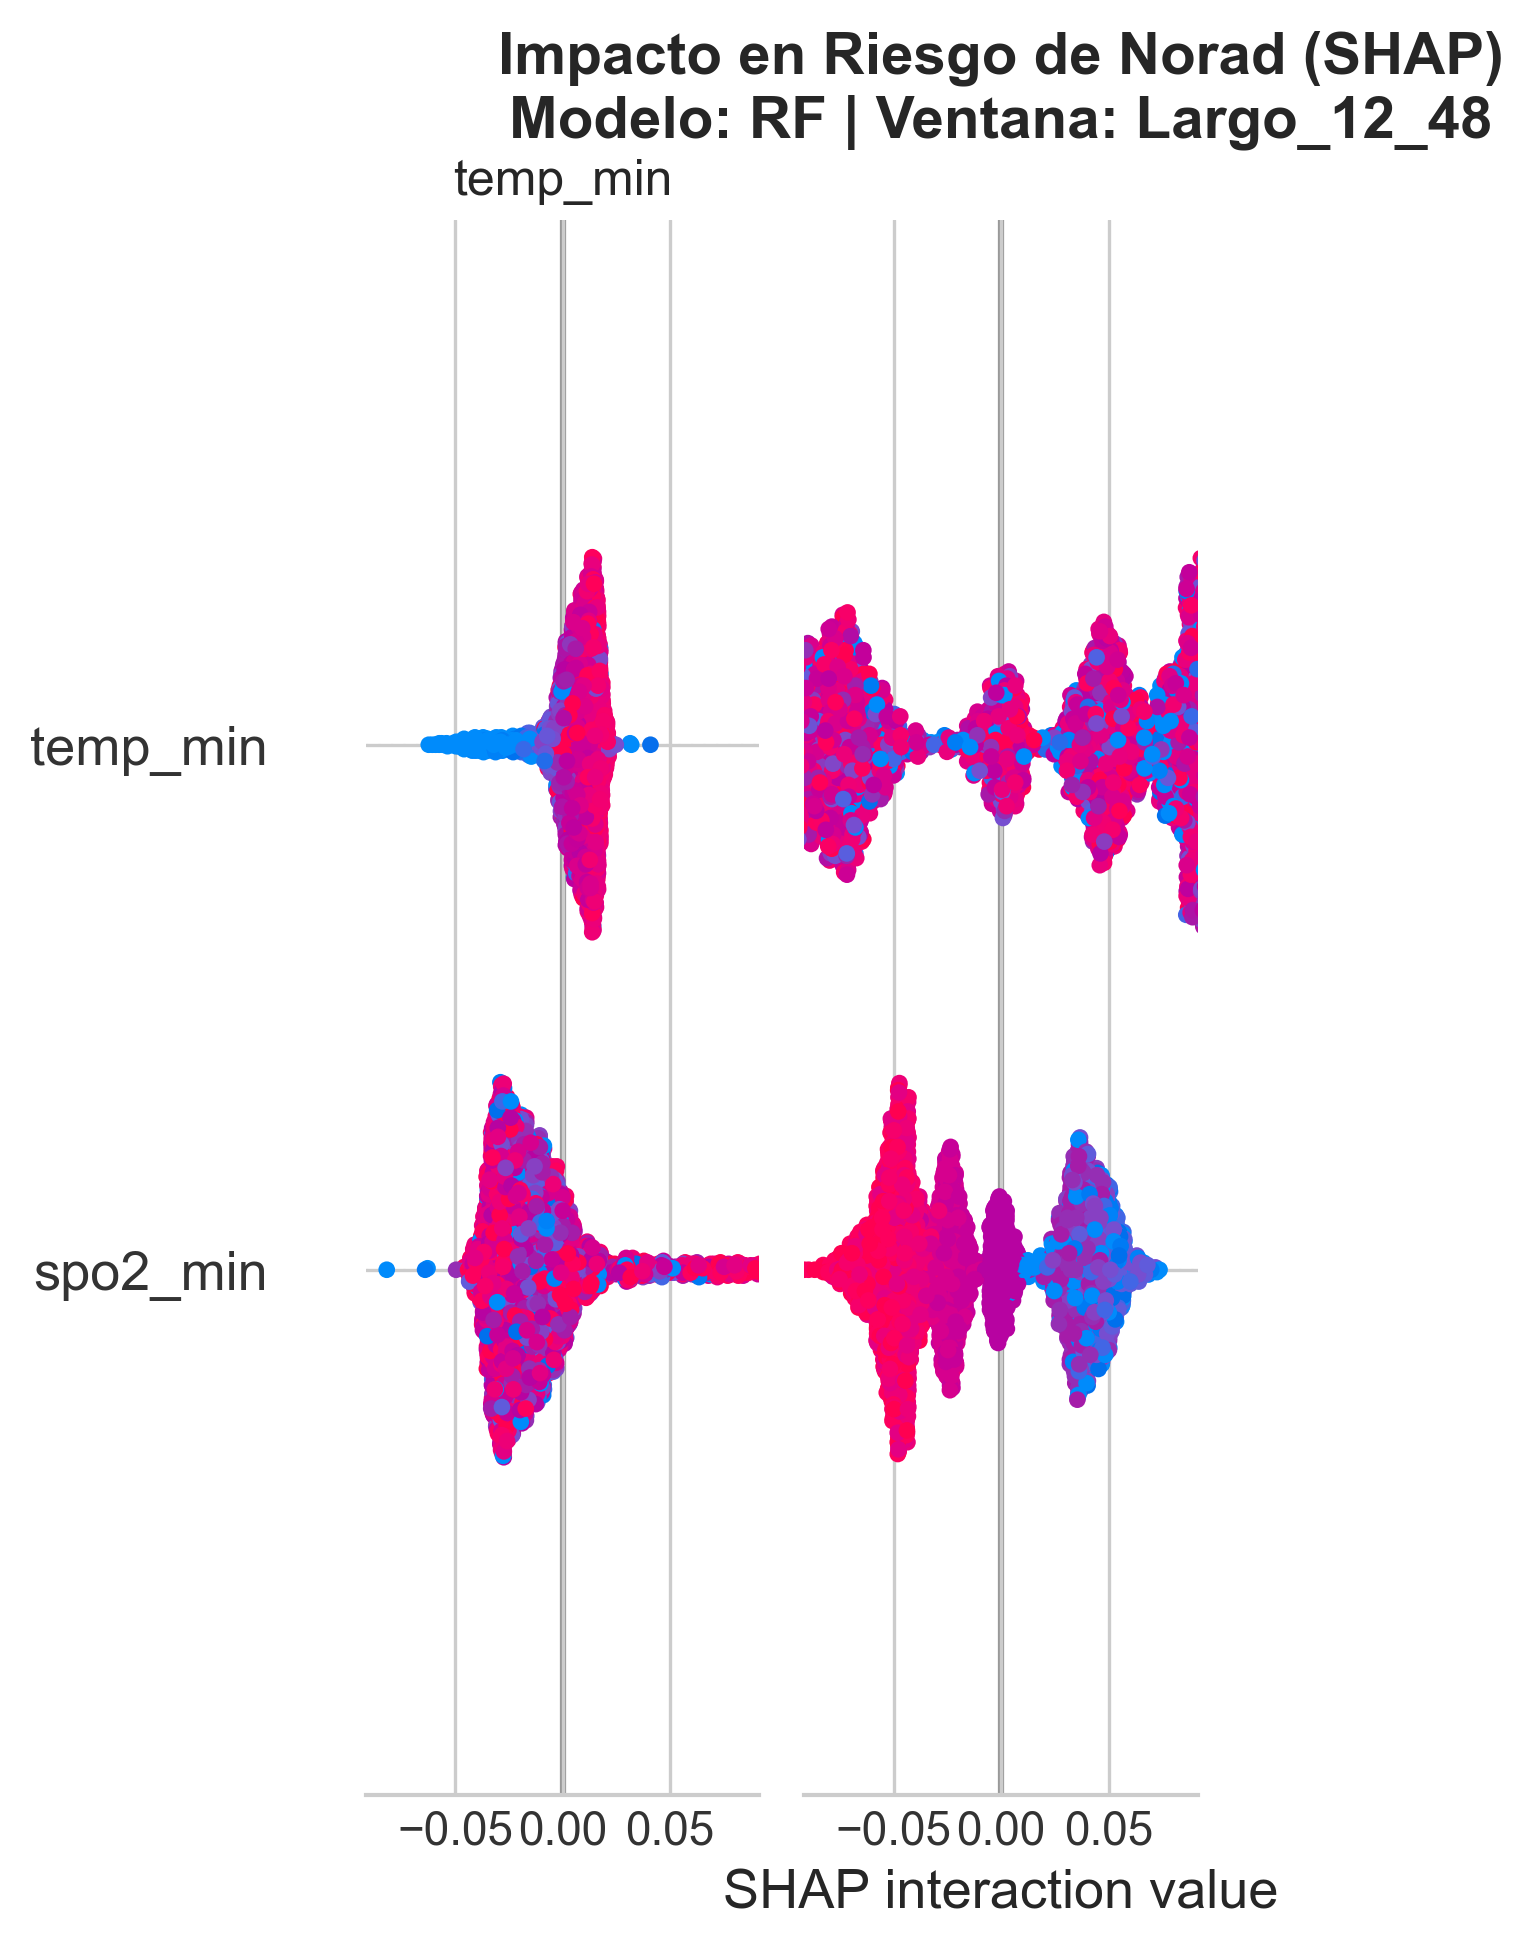
\includegraphics[width=\linewidth]{img/SHAP_Largo_12_48_RF.png}\caption{Random Forest}\end{subfigure}\hfill
  \begin{subfigure}[t]{0.48\textwidth}\centering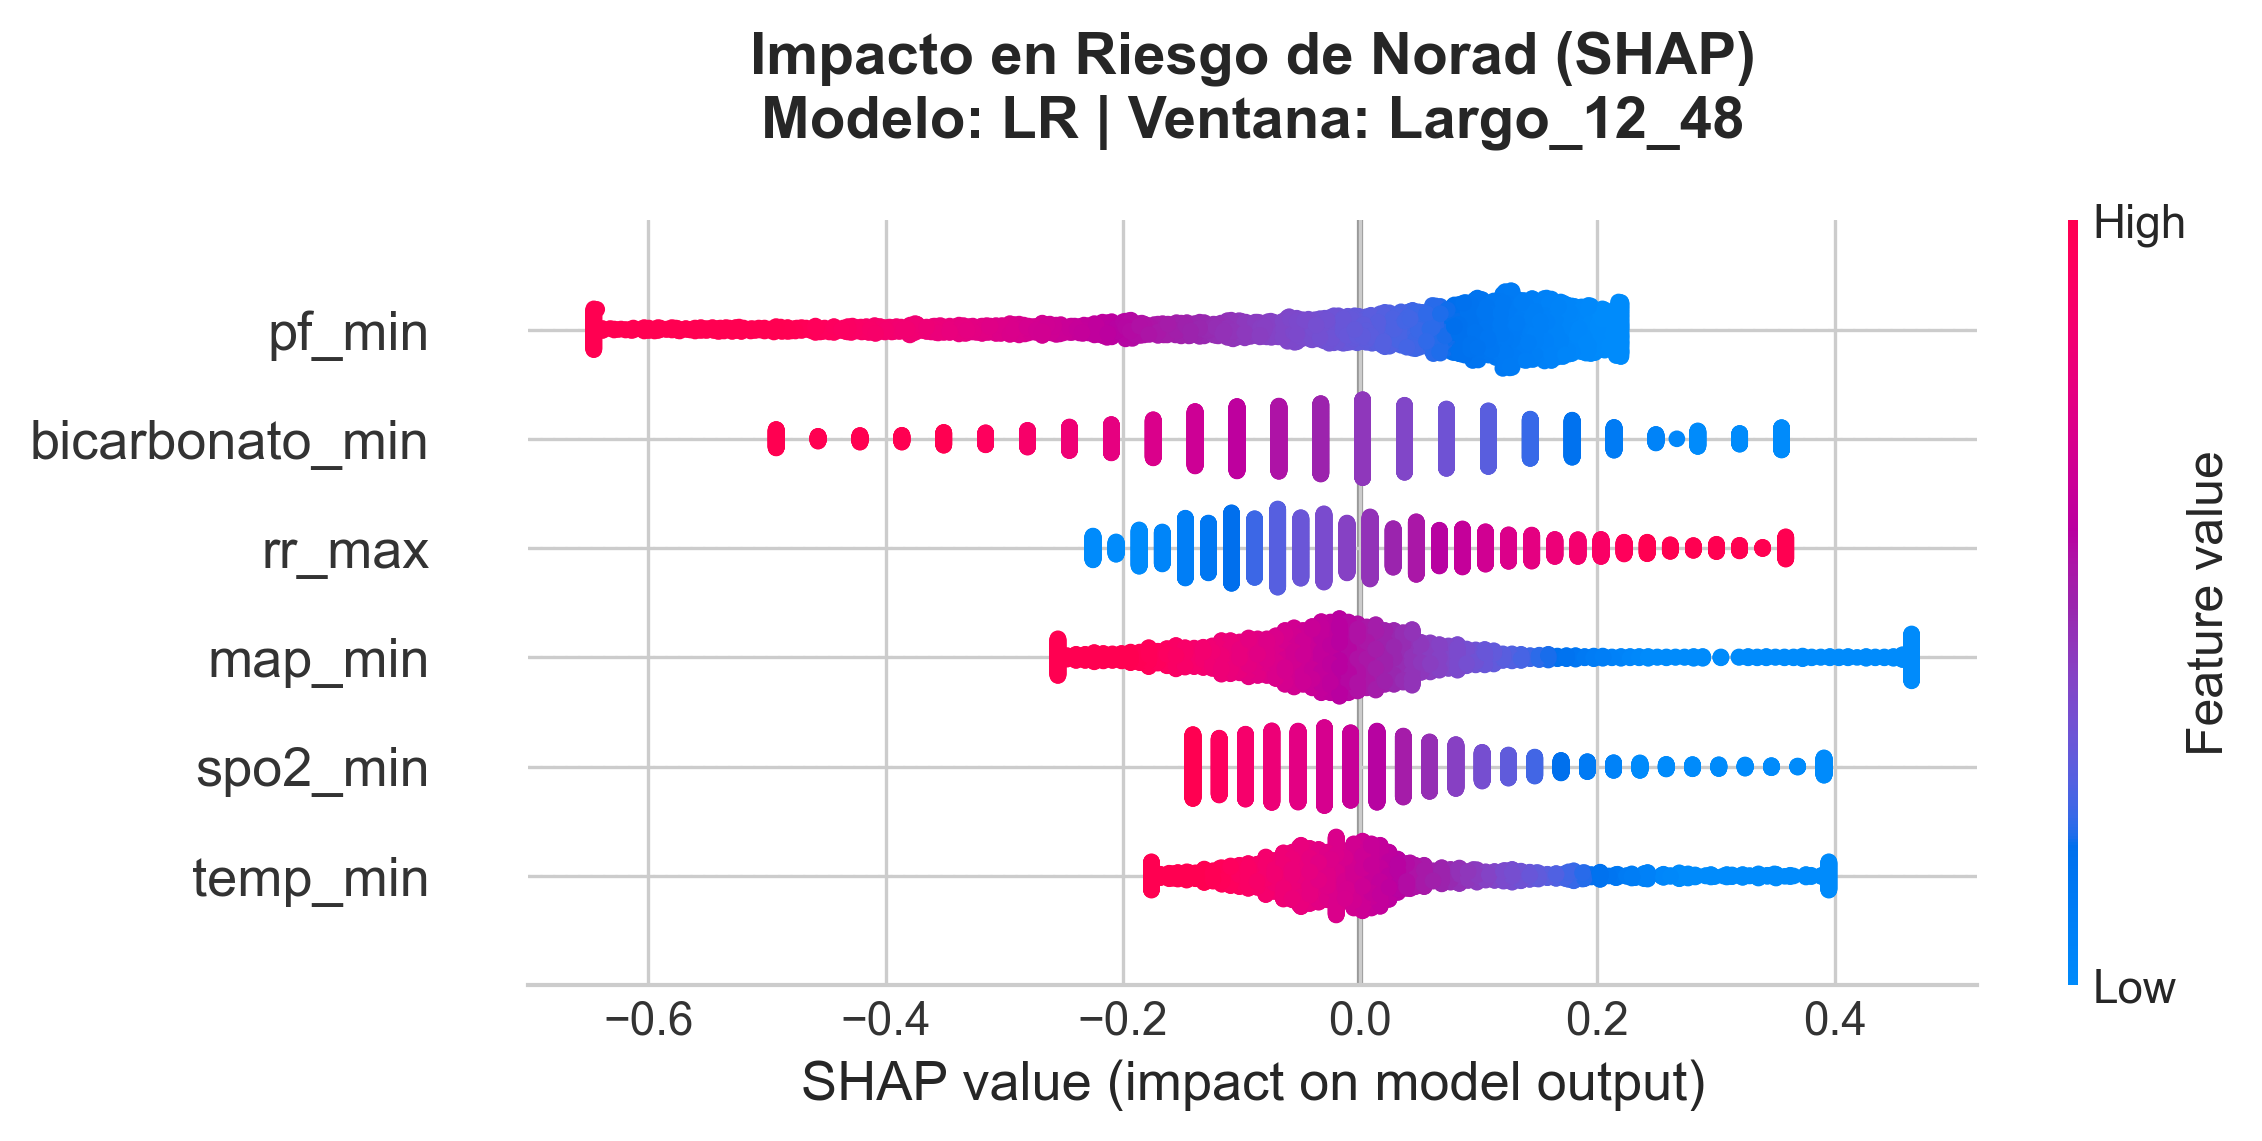
\includegraphics[width=\linewidth]{img/SHAP_Largo_12_48_LR.png}\caption{Regresión logística}\end{subfigure}\\[6pt]
  \begin{subfigure}[t]{0.48\textwidth}\centering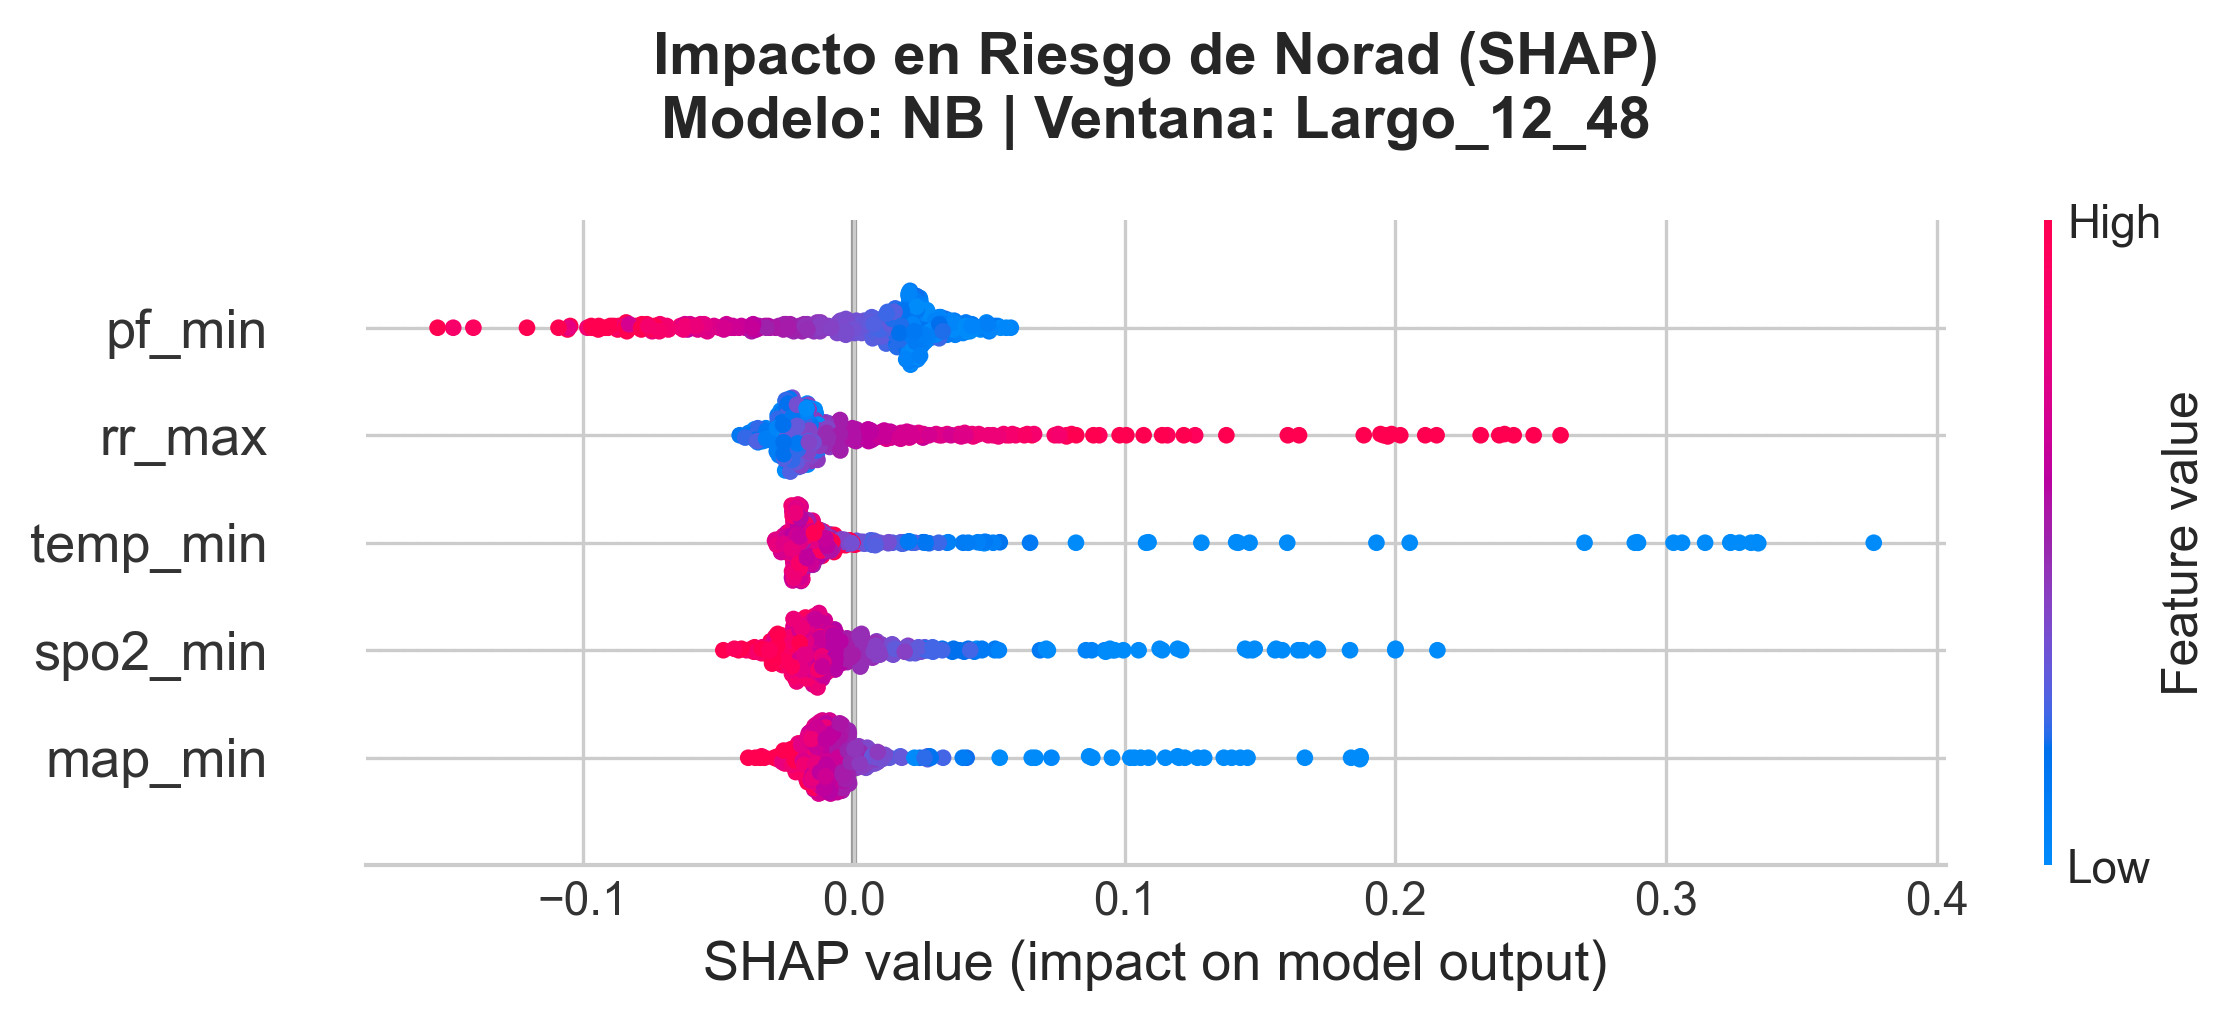
\includegraphics[width=\linewidth]{img/SHAP_Largo_12_48_NB.png}\caption{Naive Bayes}\end{subfigure}
  \caption{Diagramas SHAP de los modelos en la ventana larga (12--48\,h), MIMIC-IV.}
  \label{fig:shap-largo}
\end{figure}
 
\subsubsection*{Validación externa (eICU-CRD): discriminación y calibración}

La figura~\ref{fig:ext-roc} reúne las curvas ROC y de calibración de los modelos
evaluados en eICU-CRD frente a SOFA. Las etiquetas \emph{(cal.)} indican el
XGBoost calibrado de la ventana media.
 
\begin{figure}[htbp]
  \centering
  \begin{subfigure}[t]{0.48\textwidth}\centering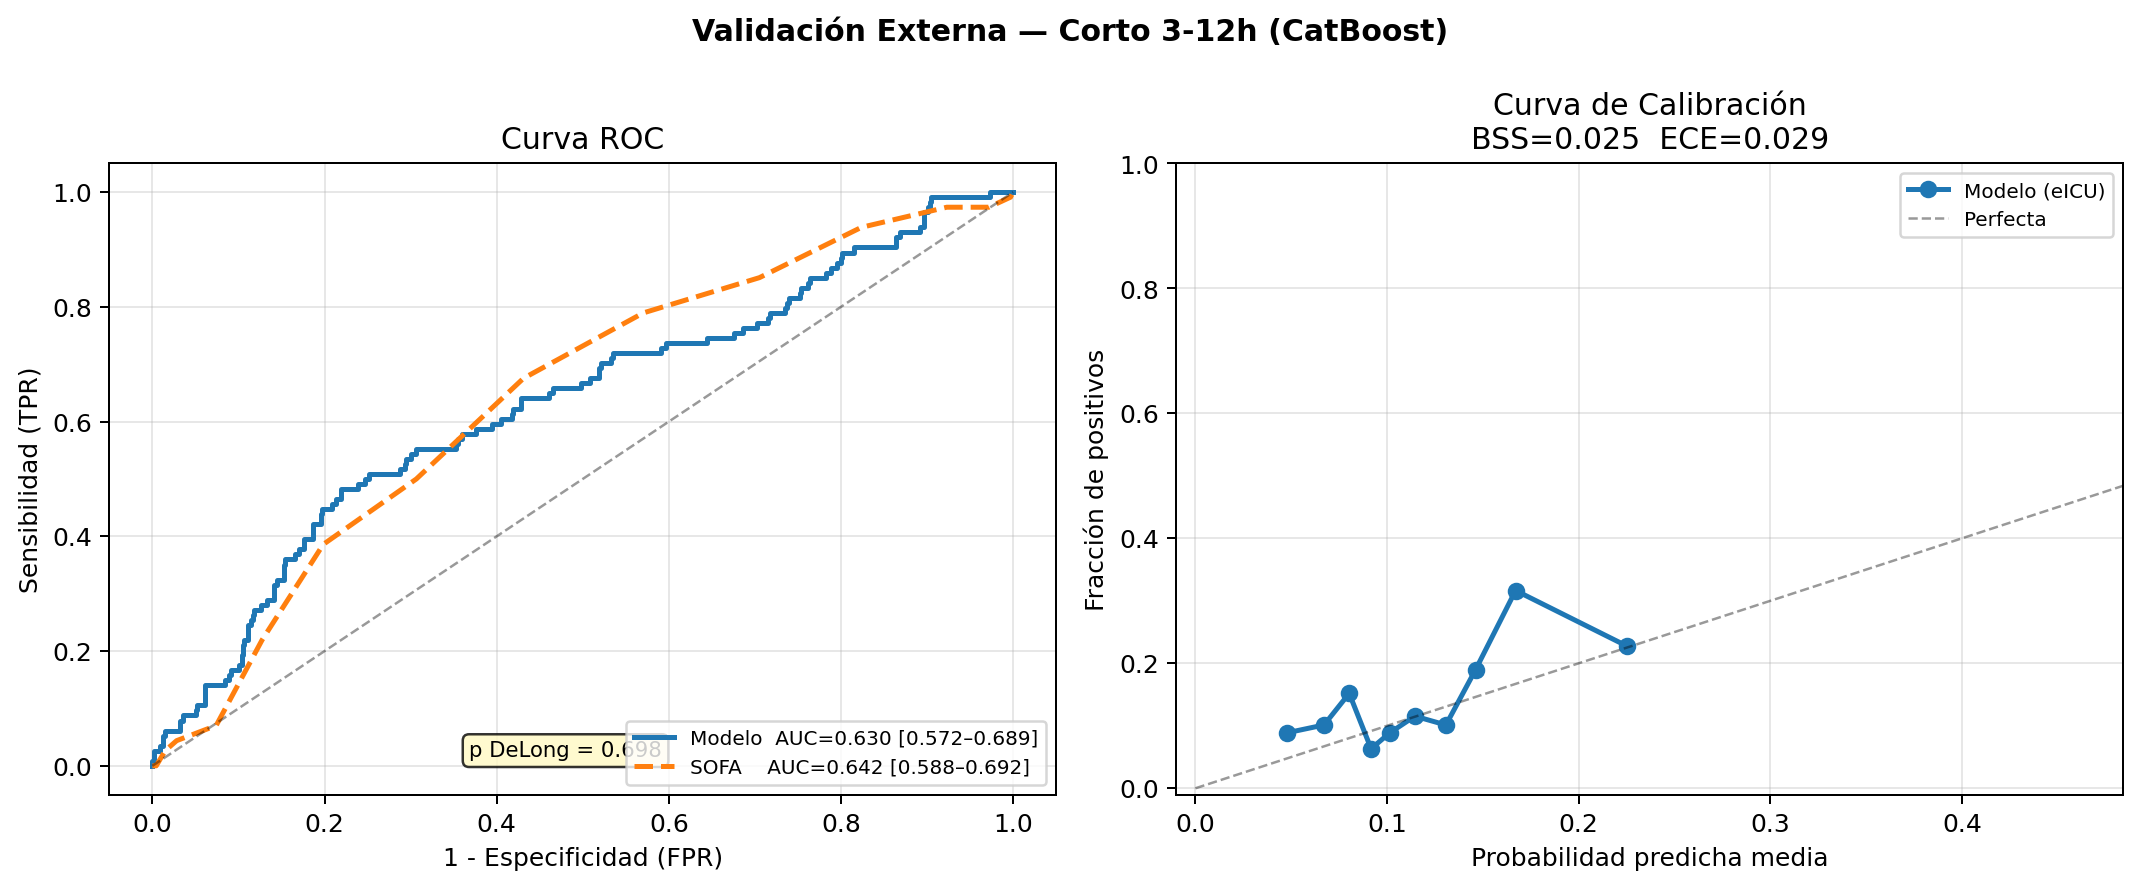
\includegraphics[width=\linewidth]{img/validacion_externa_Corto_3_12.png}\caption{Corta — CatBoost}\end{subfigure}\hfill
  \begin{subfigure}[t]{0.48\textwidth}\centering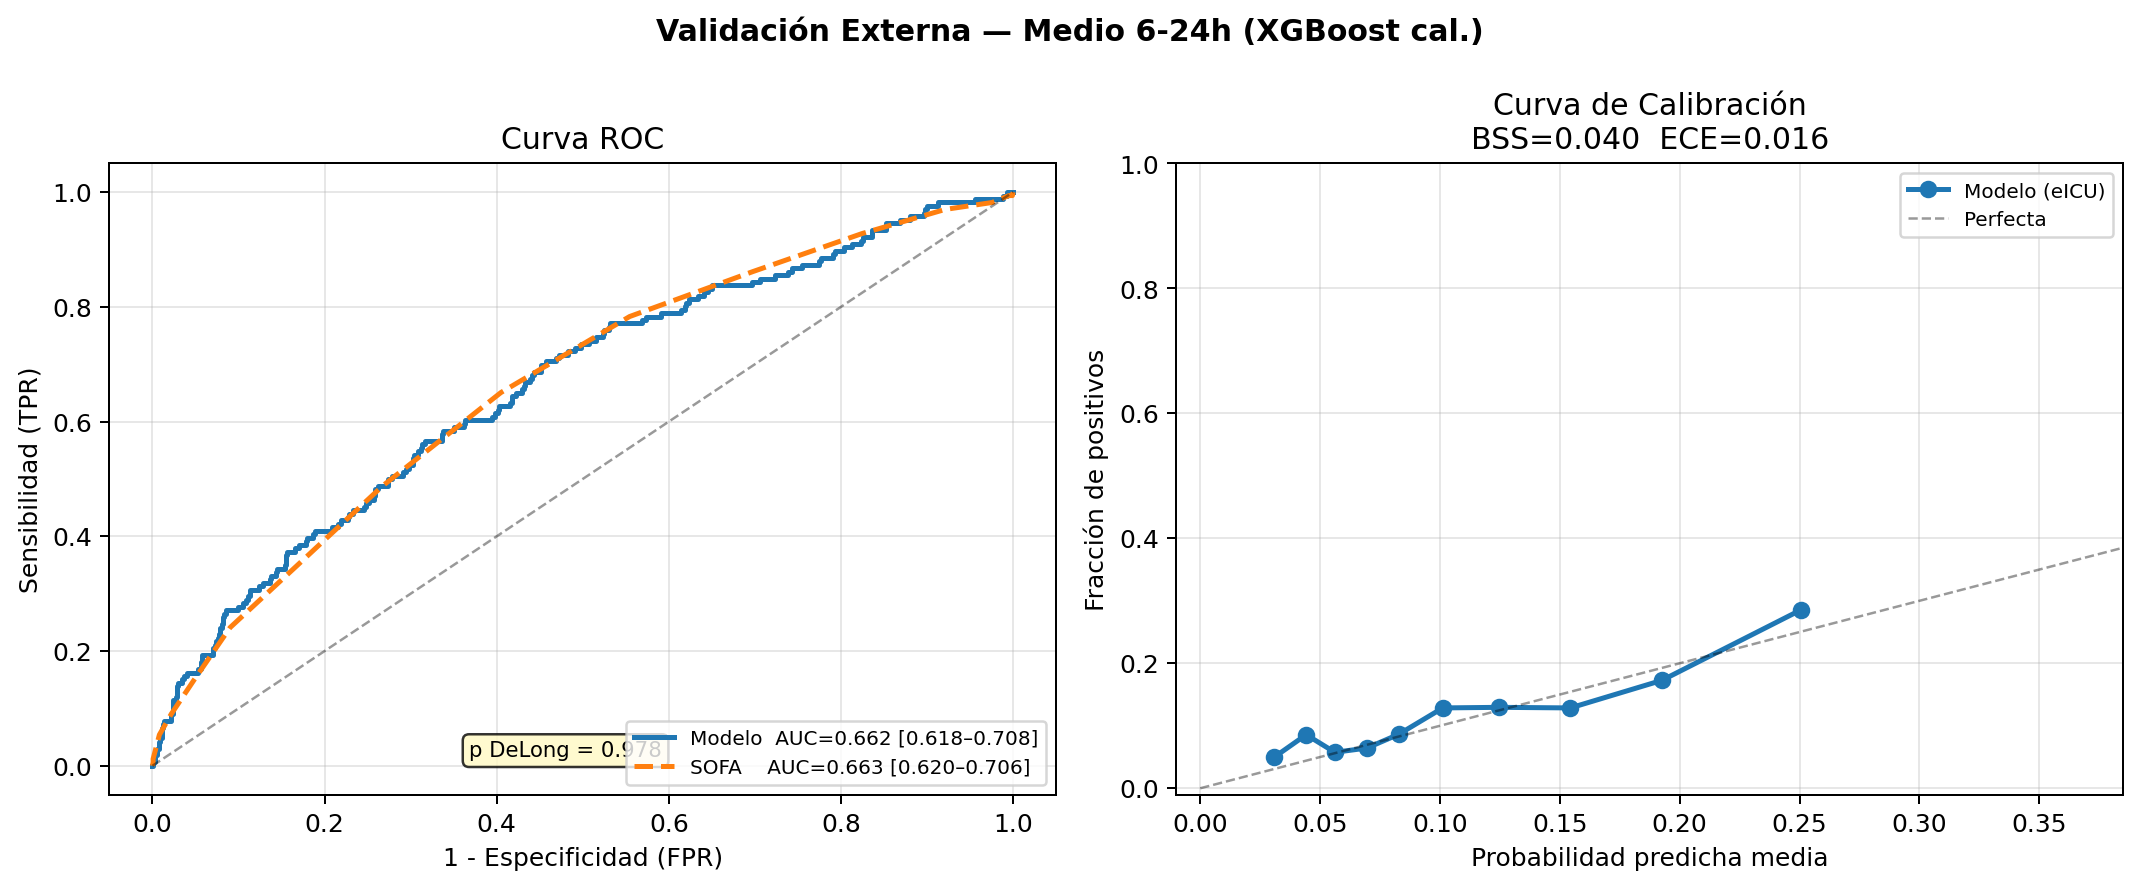
\includegraphics[width=\linewidth]{img/validacion_externa_Medio_6_24.png}\caption{Media — XGBoost cal.}\end{subfigure}\\[6pt]
  \begin{subfigure}[t]{0.48\textwidth}\centering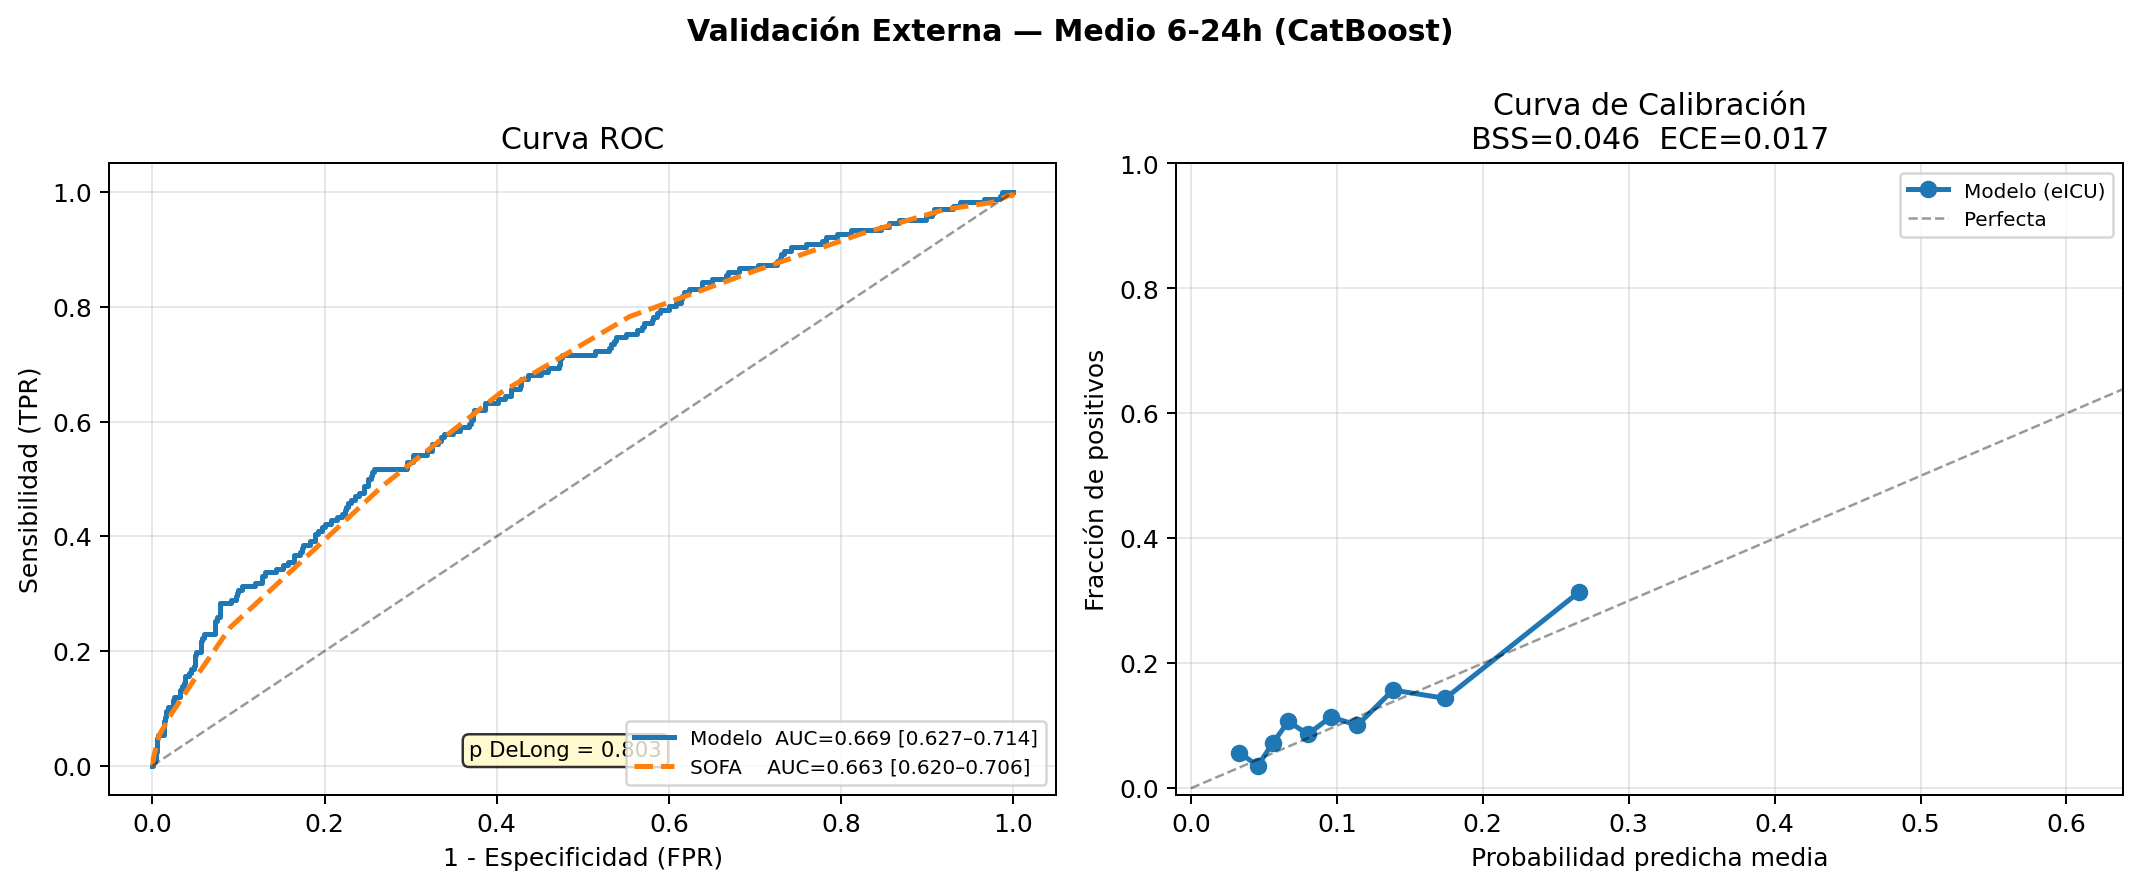
\includegraphics[width=\linewidth]{img/validacion_externa_Medio_6_24_CAT.png}\caption{Media — CatBoost}\end{subfigure}\hfill
  \begin{subfigure}[t]{0.48\textwidth}\centering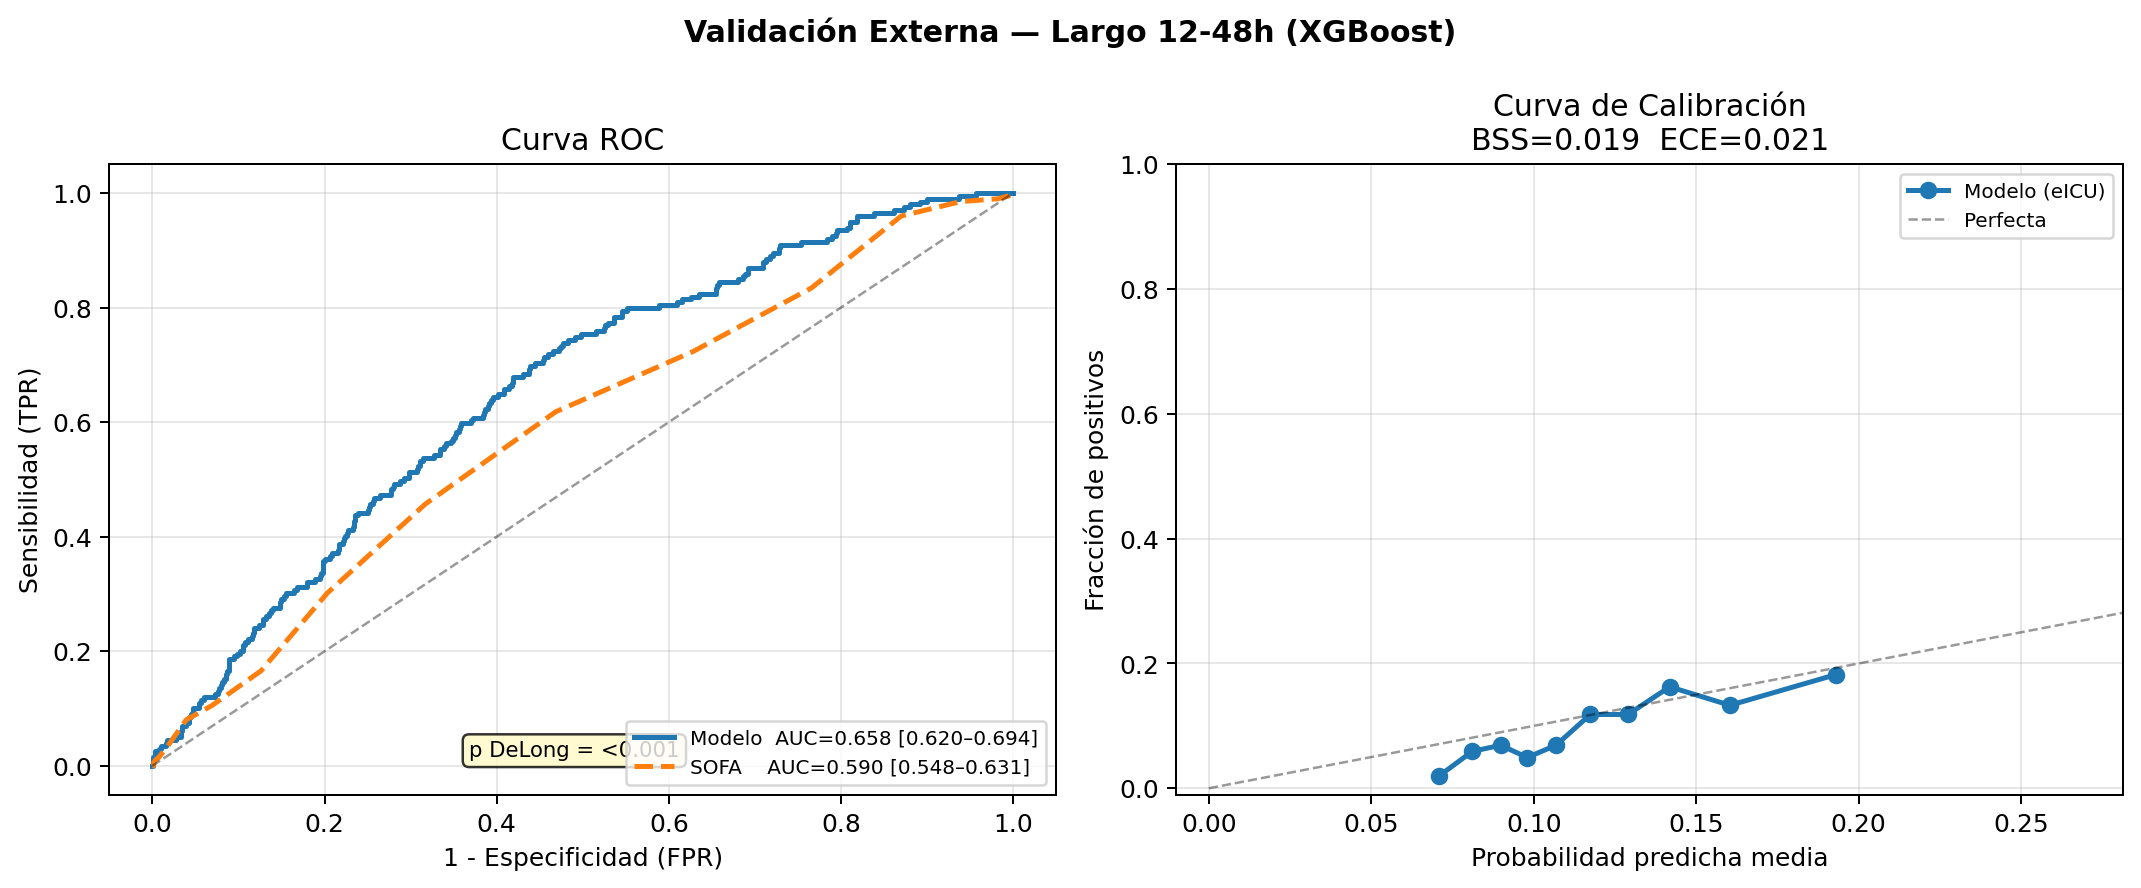
\includegraphics[width=\linewidth]{img/validacion_externa_Largo_12_48.png}\caption{Larga — XGBoost}\end{subfigure}\\[6pt]
  \begin{subfigure}[t]{0.48\textwidth}\centering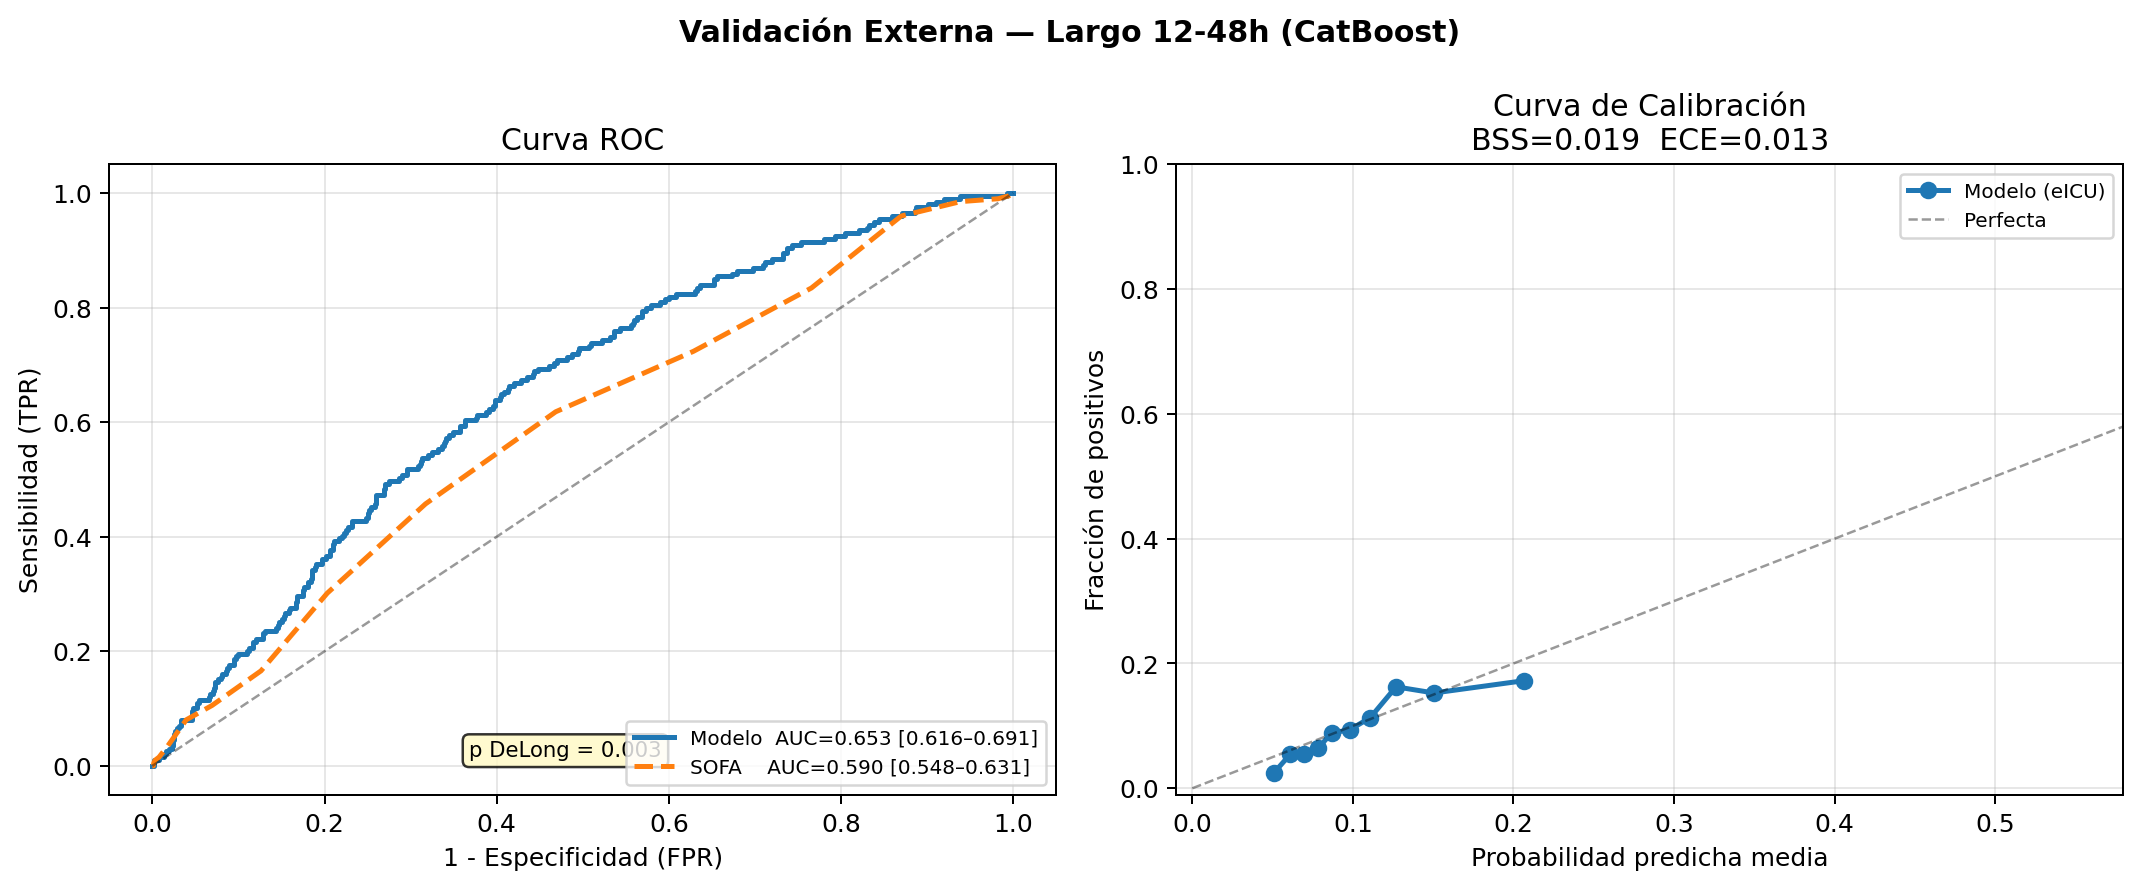
\includegraphics[width=\linewidth]{img/validacion_externa_Largo_12_48_CAT.png}\caption{Larga — CatBoost}\end{subfigure}
  \caption{Validación externa en eICU-CRD: curvas ROC y de calibración de cada modelo y ventana.}
  \label{fig:ext-roc}
\end{figure}
 
\subsubsection*{Validación externa (eICU-CRD): diagramas SHAP}

La figura~\ref{fig:ext-shap} recoge los diagramas SHAP calculados sobre la cohorte
externa, que permiten comprobar la consistencia del comportamiento del modelo
entre MIMIC-IV y eICU-CRD.
 
\begin{figure}[htbp]
  \centering
  \begin{subfigure}[t]{0.48\textwidth}\centering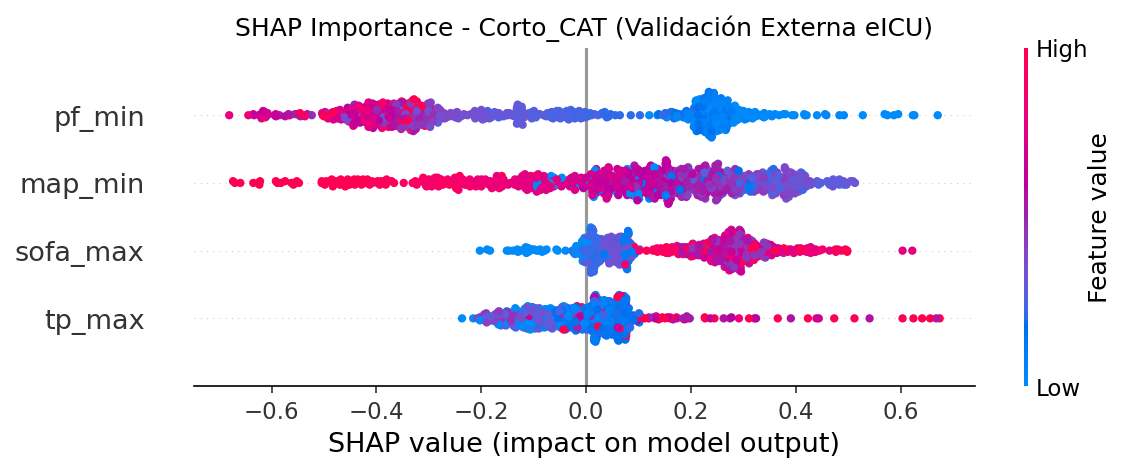
\includegraphics[width=\linewidth]{img/shap_eicu_corto_cat.png}\caption{Corta — CatBoost}\end{subfigure}\hfill
  \begin{subfigure}[t]{0.48\textwidth}\centering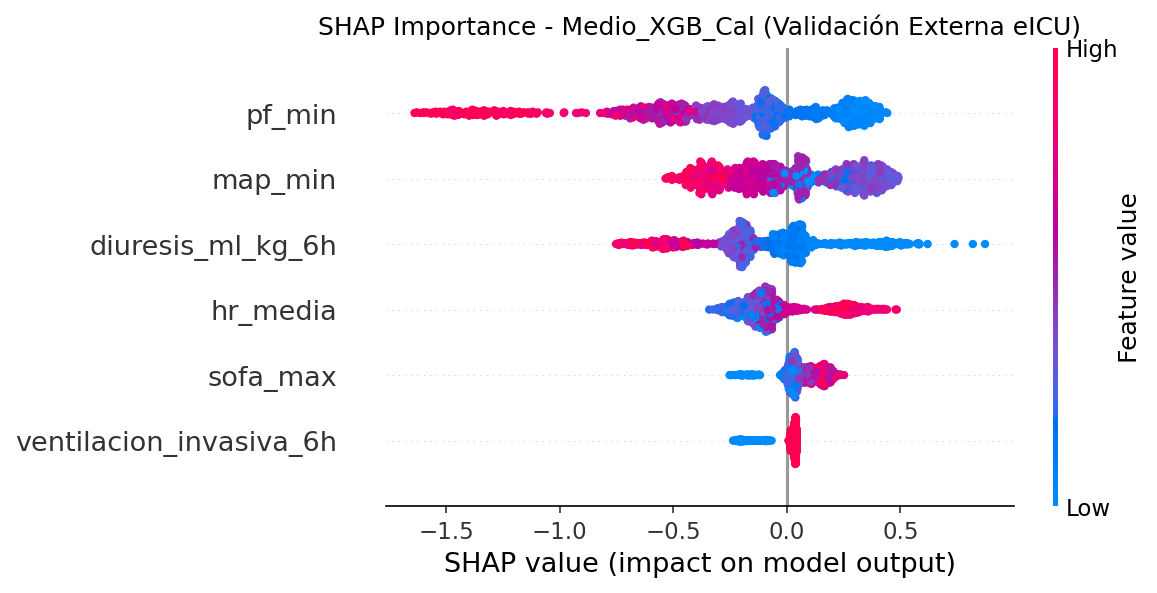
\includegraphics[width=\linewidth]{img/shap_eicu_medio_xgb_cal.png}\caption{Media — XGBoost cal.}\end{subfigure}\\[6pt]
  \begin{subfigure}[t]{0.48\textwidth}\centering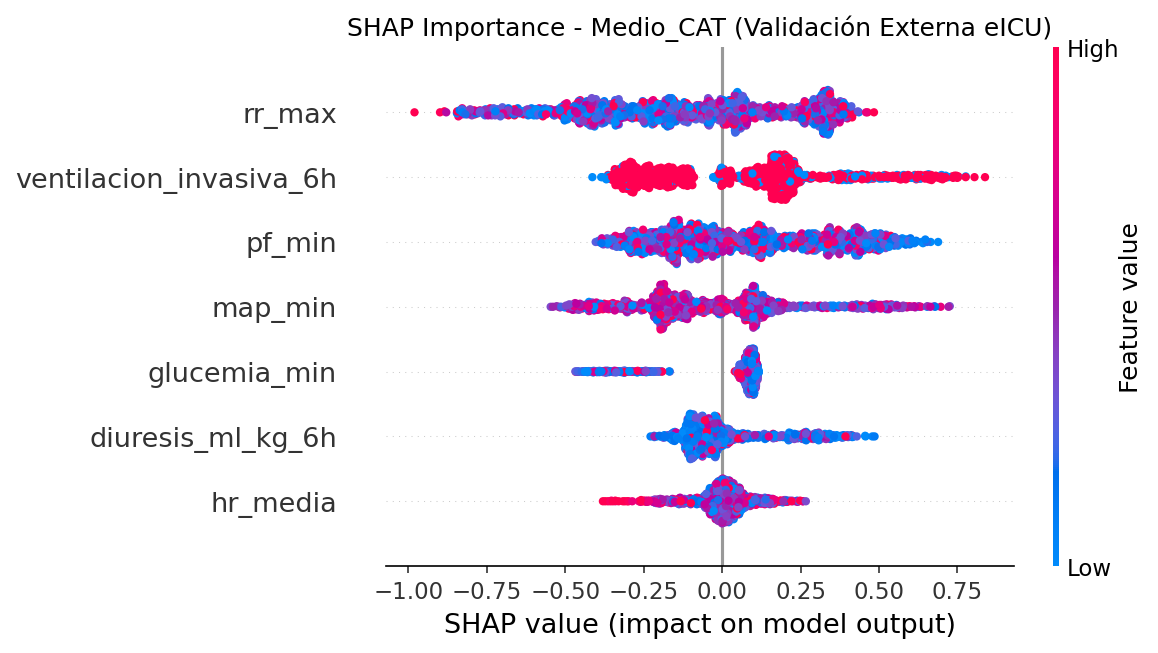
\includegraphics[width=\linewidth]{img/shap_eicu_medio_cat.png}\caption{Media — CatBoost}\end{subfigure}\hfill
  \begin{subfigure}[t]{0.48\textwidth}\centering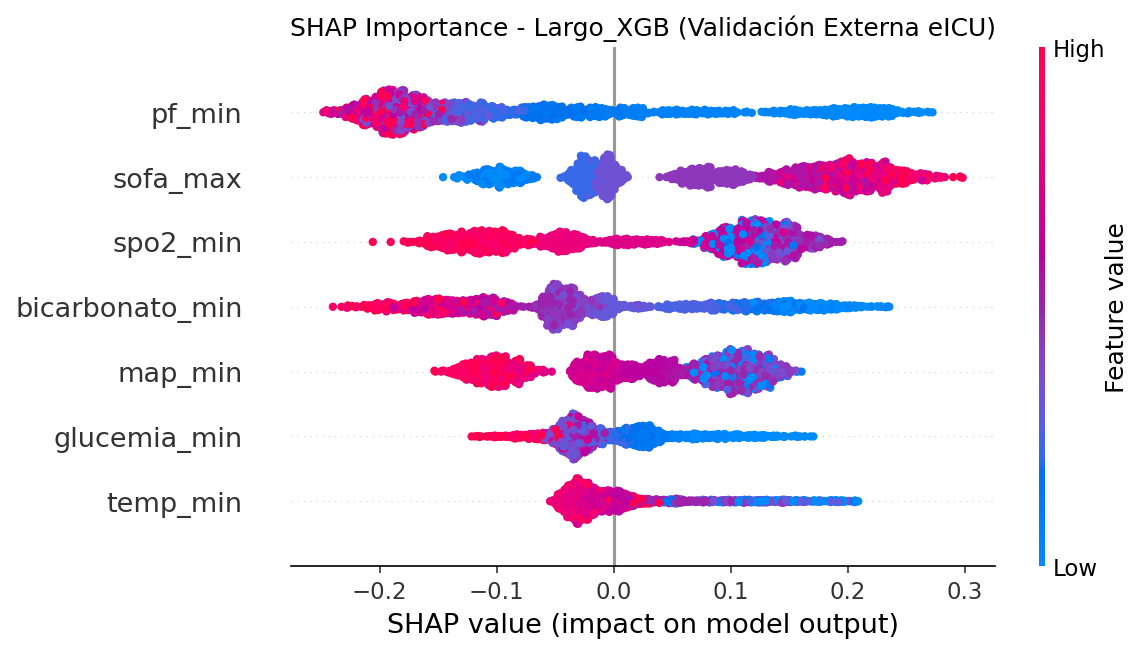
\includegraphics[width=\linewidth]{img/shap_eicu_largo_xgb.png}\caption{Larga — XGBoost}\end{subfigure}\\[6pt]
  \begin{subfigure}[t]{0.48\textwidth}\centering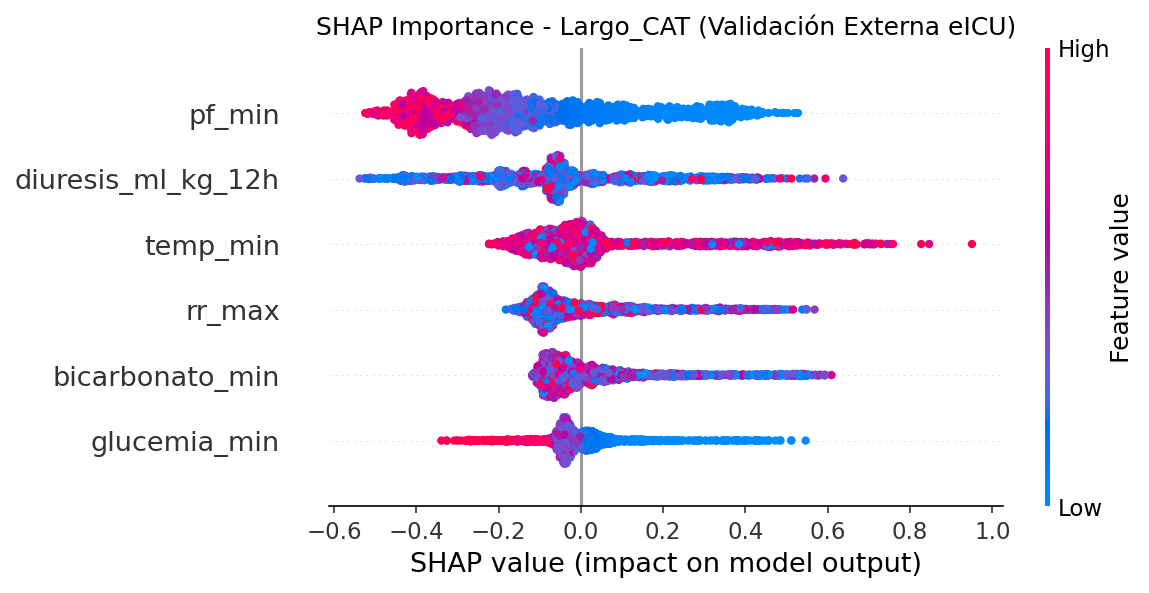
\includegraphics[width=\linewidth]{img/shap_eicu_largo_cat.png}\caption{Larga — CatBoost}\end{subfigure}
  \caption{Diagramas SHAP de los modelos sobre la cohorte de validación externa eICU-CRD.}
  \label{fig:ext-shap}
\end{figure}
 
\subsubsection*{Validación externa (eICU-CRD): distribución de variables y características basales}

Las figuras~\ref{fig:eda-boxplots} y~\ref{fig:eda-boxplots-cat} comparan la
distribución de las variables del modelo entre MIMIC-IV y eICU-CRD, y la
figura~\ref{fig:tabla1} las características basales de ambas cohortes.
 
\begin{figure}[p]
  \centering
  \begin{subfigure}{\textwidth}\centering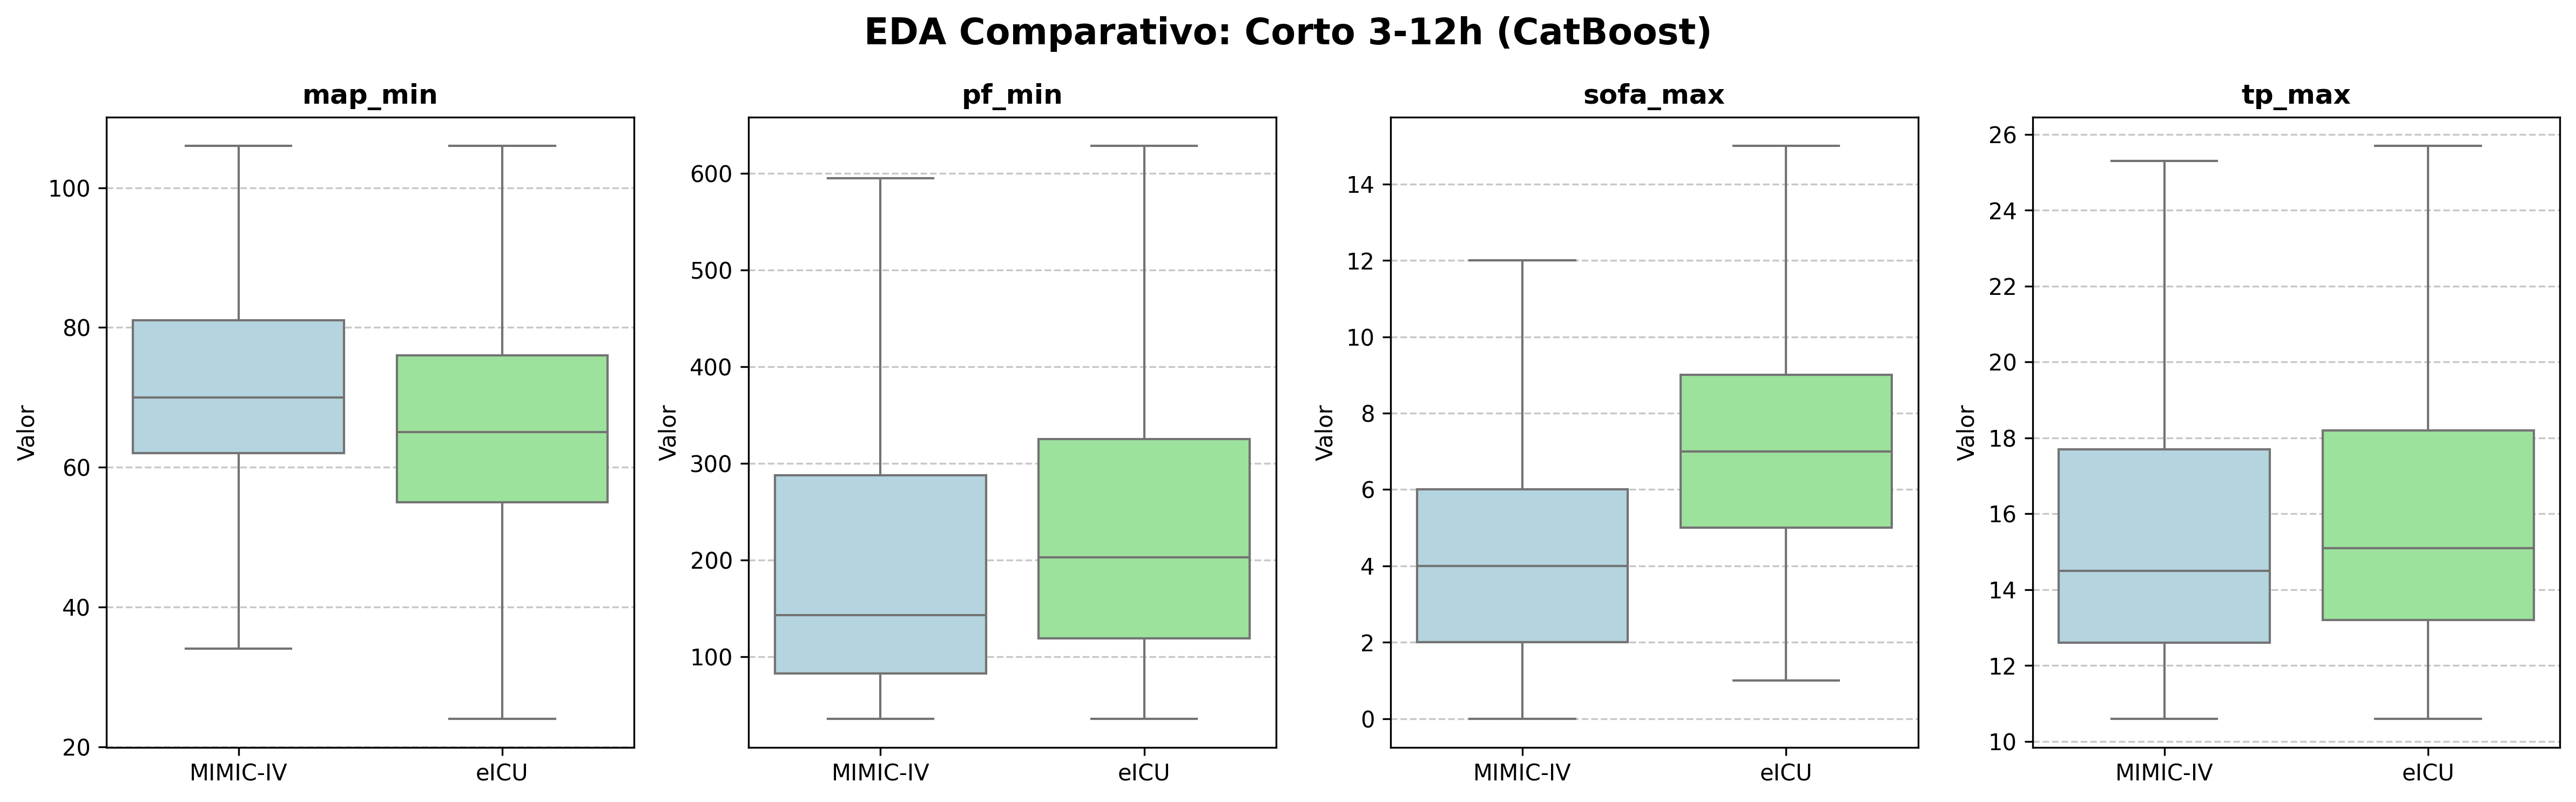
\includegraphics[width=\linewidth]{img/EDA_Boxplots_Corto_3_12.png}\caption{Ventana corta (3--12\,h)}\end{subfigure}\\[8pt]
  \begin{subfigure}{\textwidth}\centering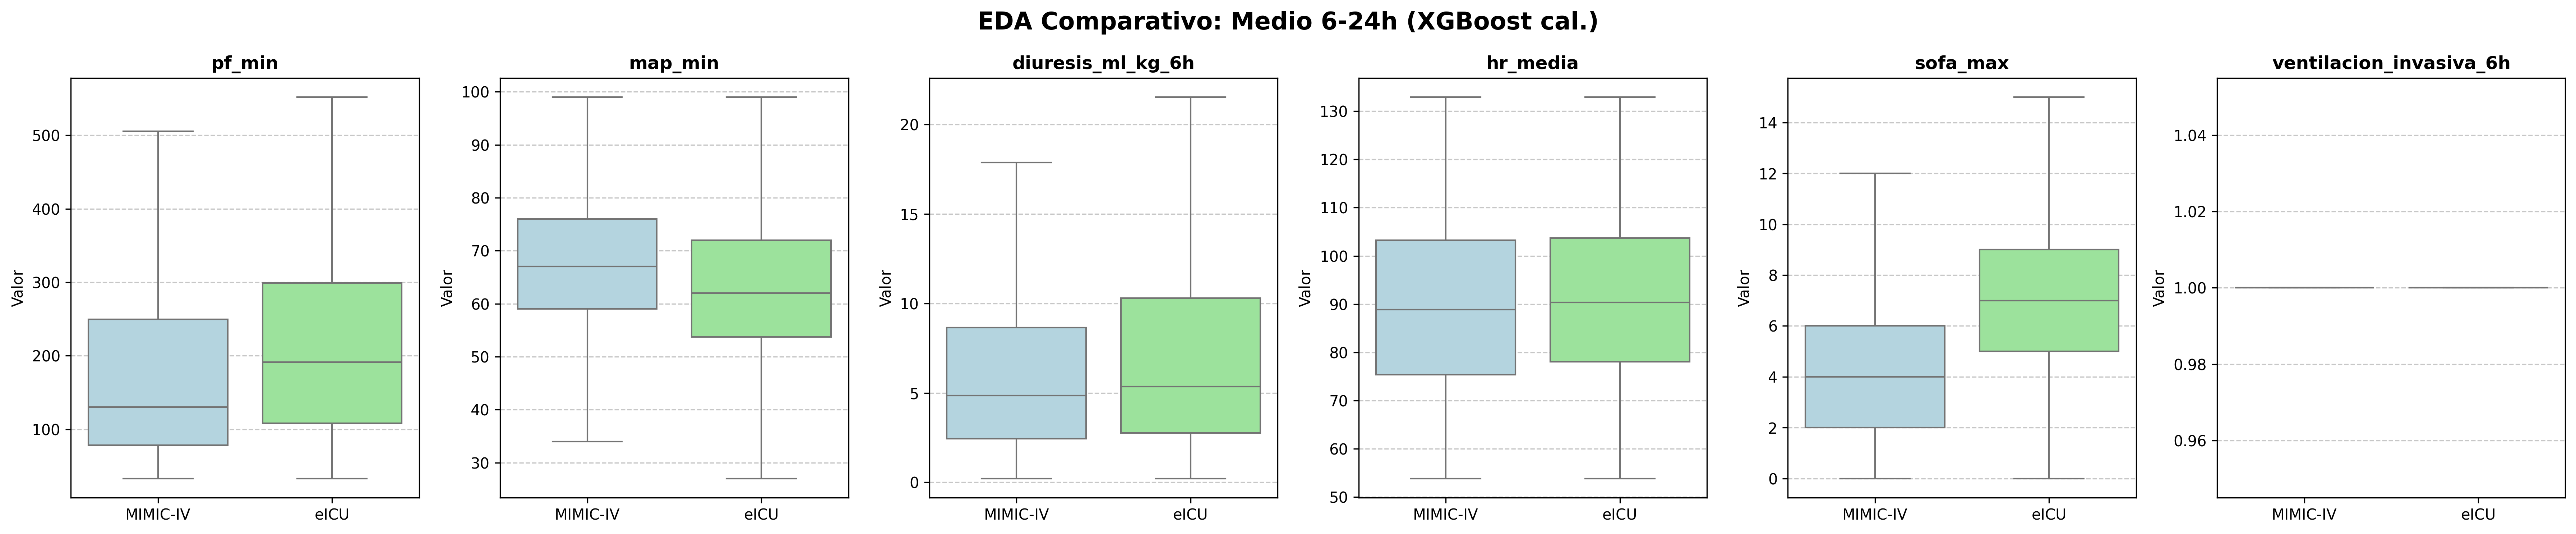
\includegraphics[width=\linewidth]{img/EDA_Boxplots_Medio_6_24.png}\caption{Ventana media (6--24\,h)}\end{subfigure}\\[8pt]
  \begin{subfigure}{\textwidth}\centering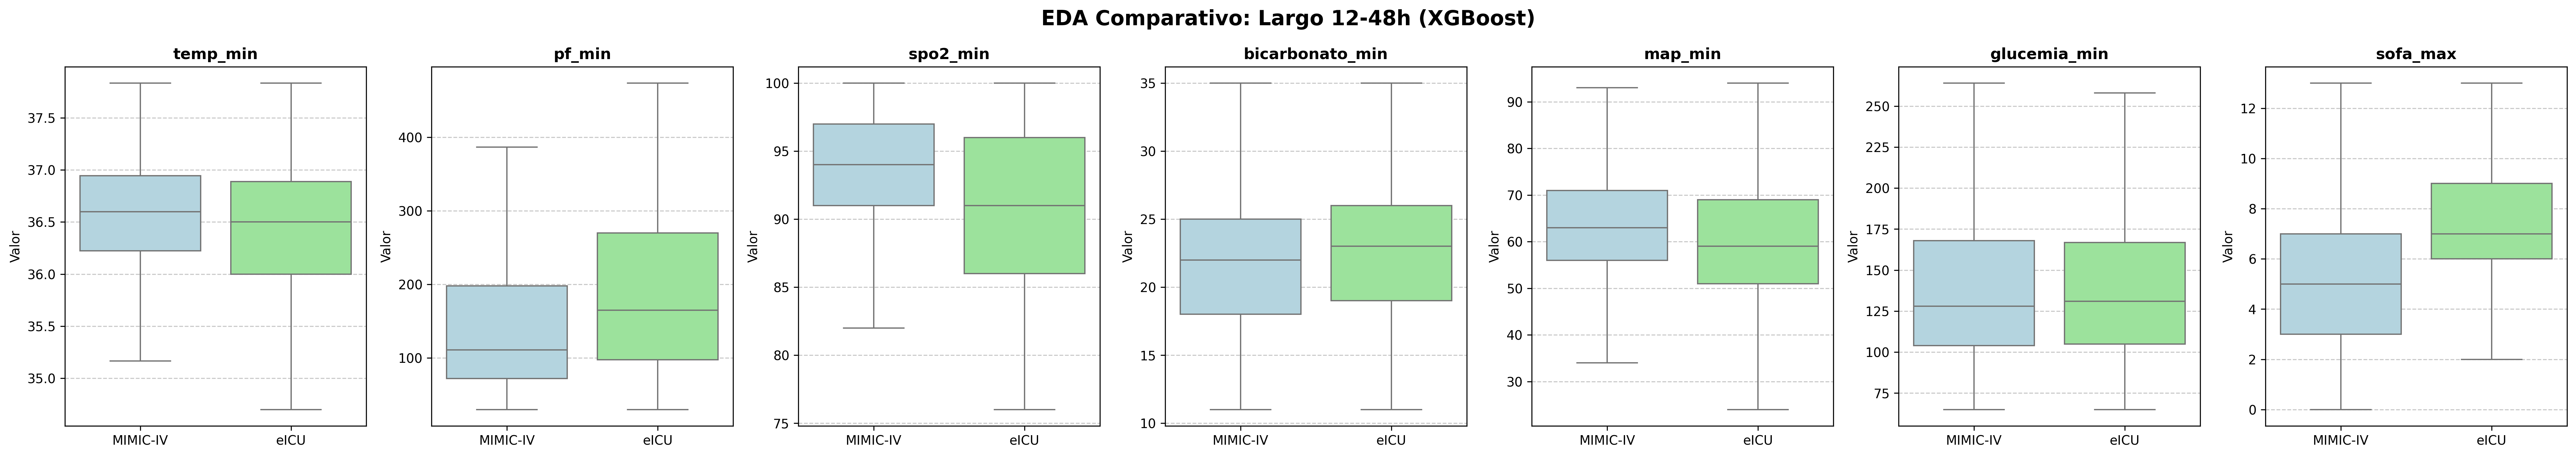
\includegraphics[width=\linewidth]{img/EDA_Boxplots_Largo_12_48.png}\caption{Ventana larga (12--48\,h)}\end{subfigure}
  \caption{Distribución comparada (diagramas de caja) de las variables predictoras
  entre MIMIC-IV (desarrollo) y eICU-CRD (validación externa). Las diferencias en
  \texttt{sofa\_max} ilustran el desplazamiento de distribución entre cohortes.}
  \label{fig:eda-boxplots}
\end{figure}
 
\begin{figure}[htbp]
  \centering
  \begin{subfigure}{\textwidth}\centering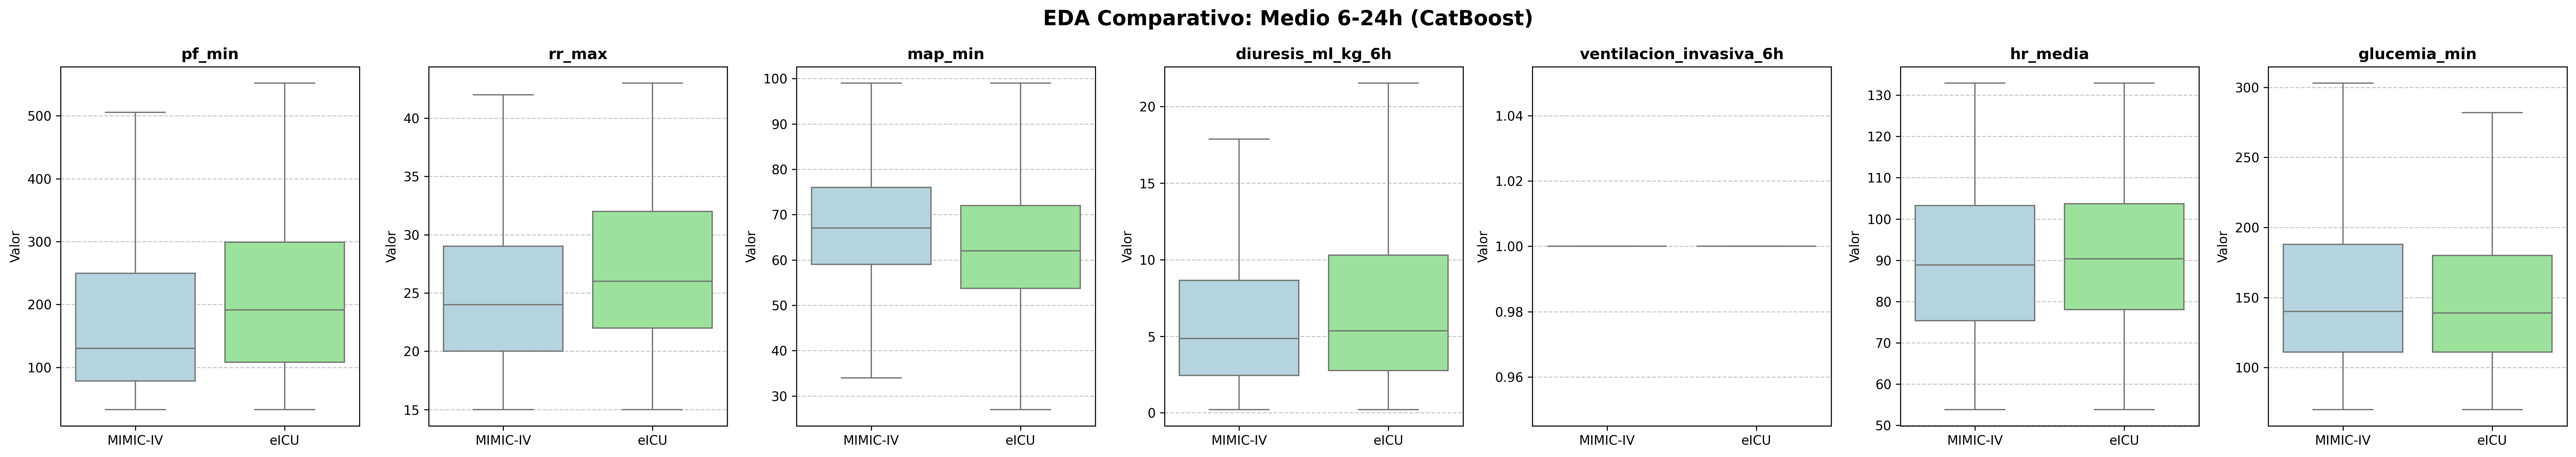
\includegraphics[width=\linewidth]{img/EDA_Boxplots_Medio_6_24_CAT.png}\caption{Ventana media (variables del CatBoost)}\end{subfigure}\\[8pt]
  \begin{subfigure}{\textwidth}\centering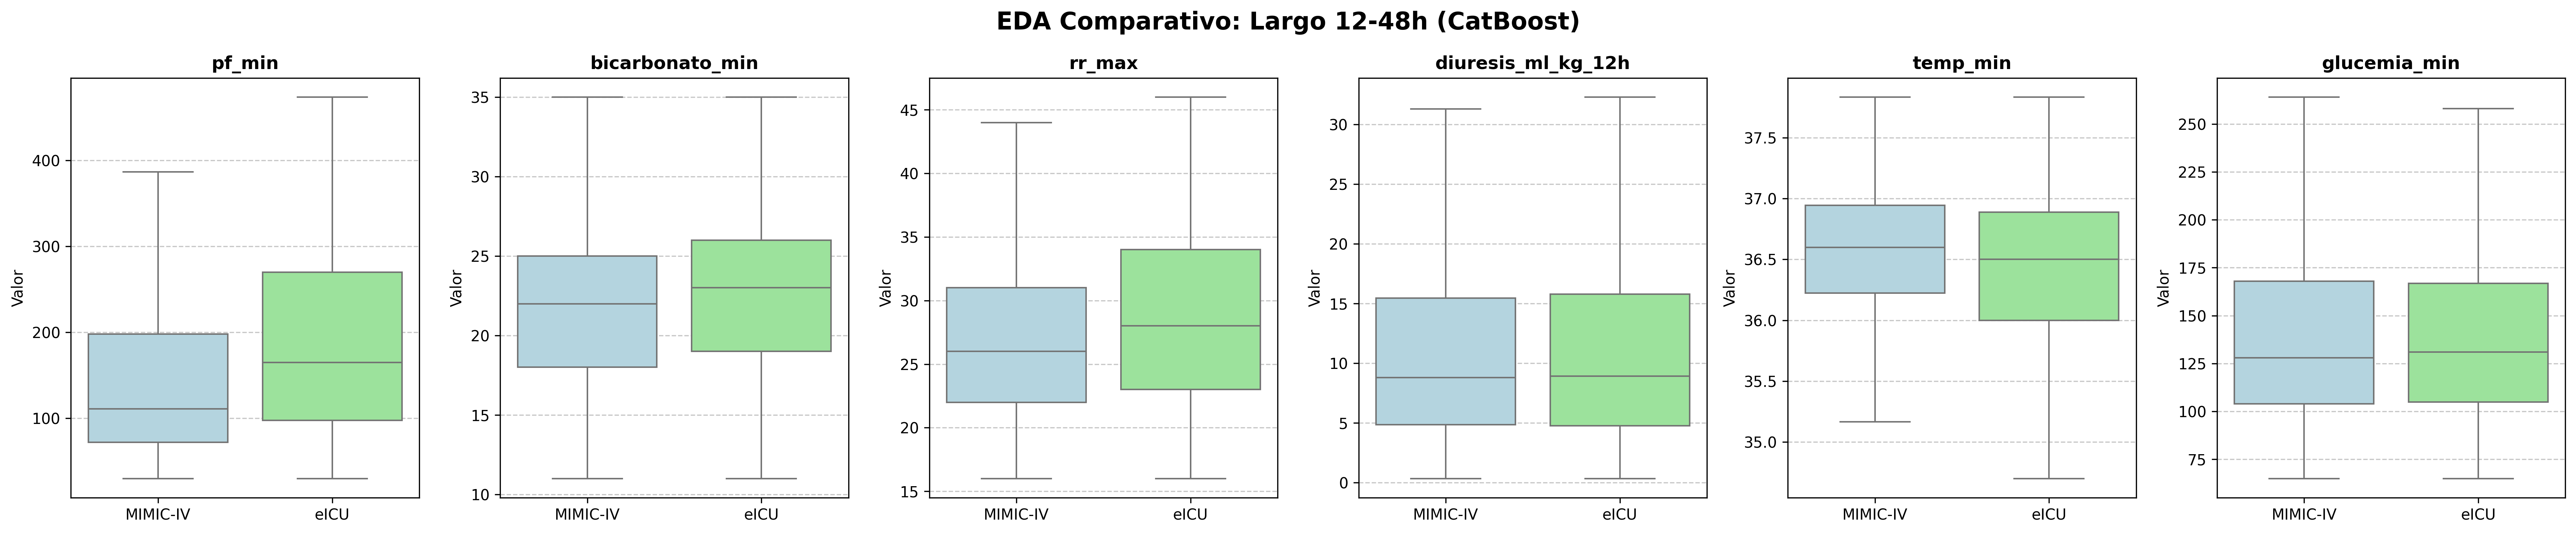
\includegraphics[width=\linewidth]{img/EDA_Boxplots_Largo_12_48_CAT.png}\caption{Ventana larga (variables del CatBoost)}\end{subfigure}
  \caption{Distribución comparada de las variables de los modelos CatBoost (segundos
  modelos de las ventanas media y larga) entre MIMIC-IV y eICU-CRD.}
  \label{fig:eda-boxplots-cat}
\end{figure}
 
\begin{figure}[htbp]
  \centering
  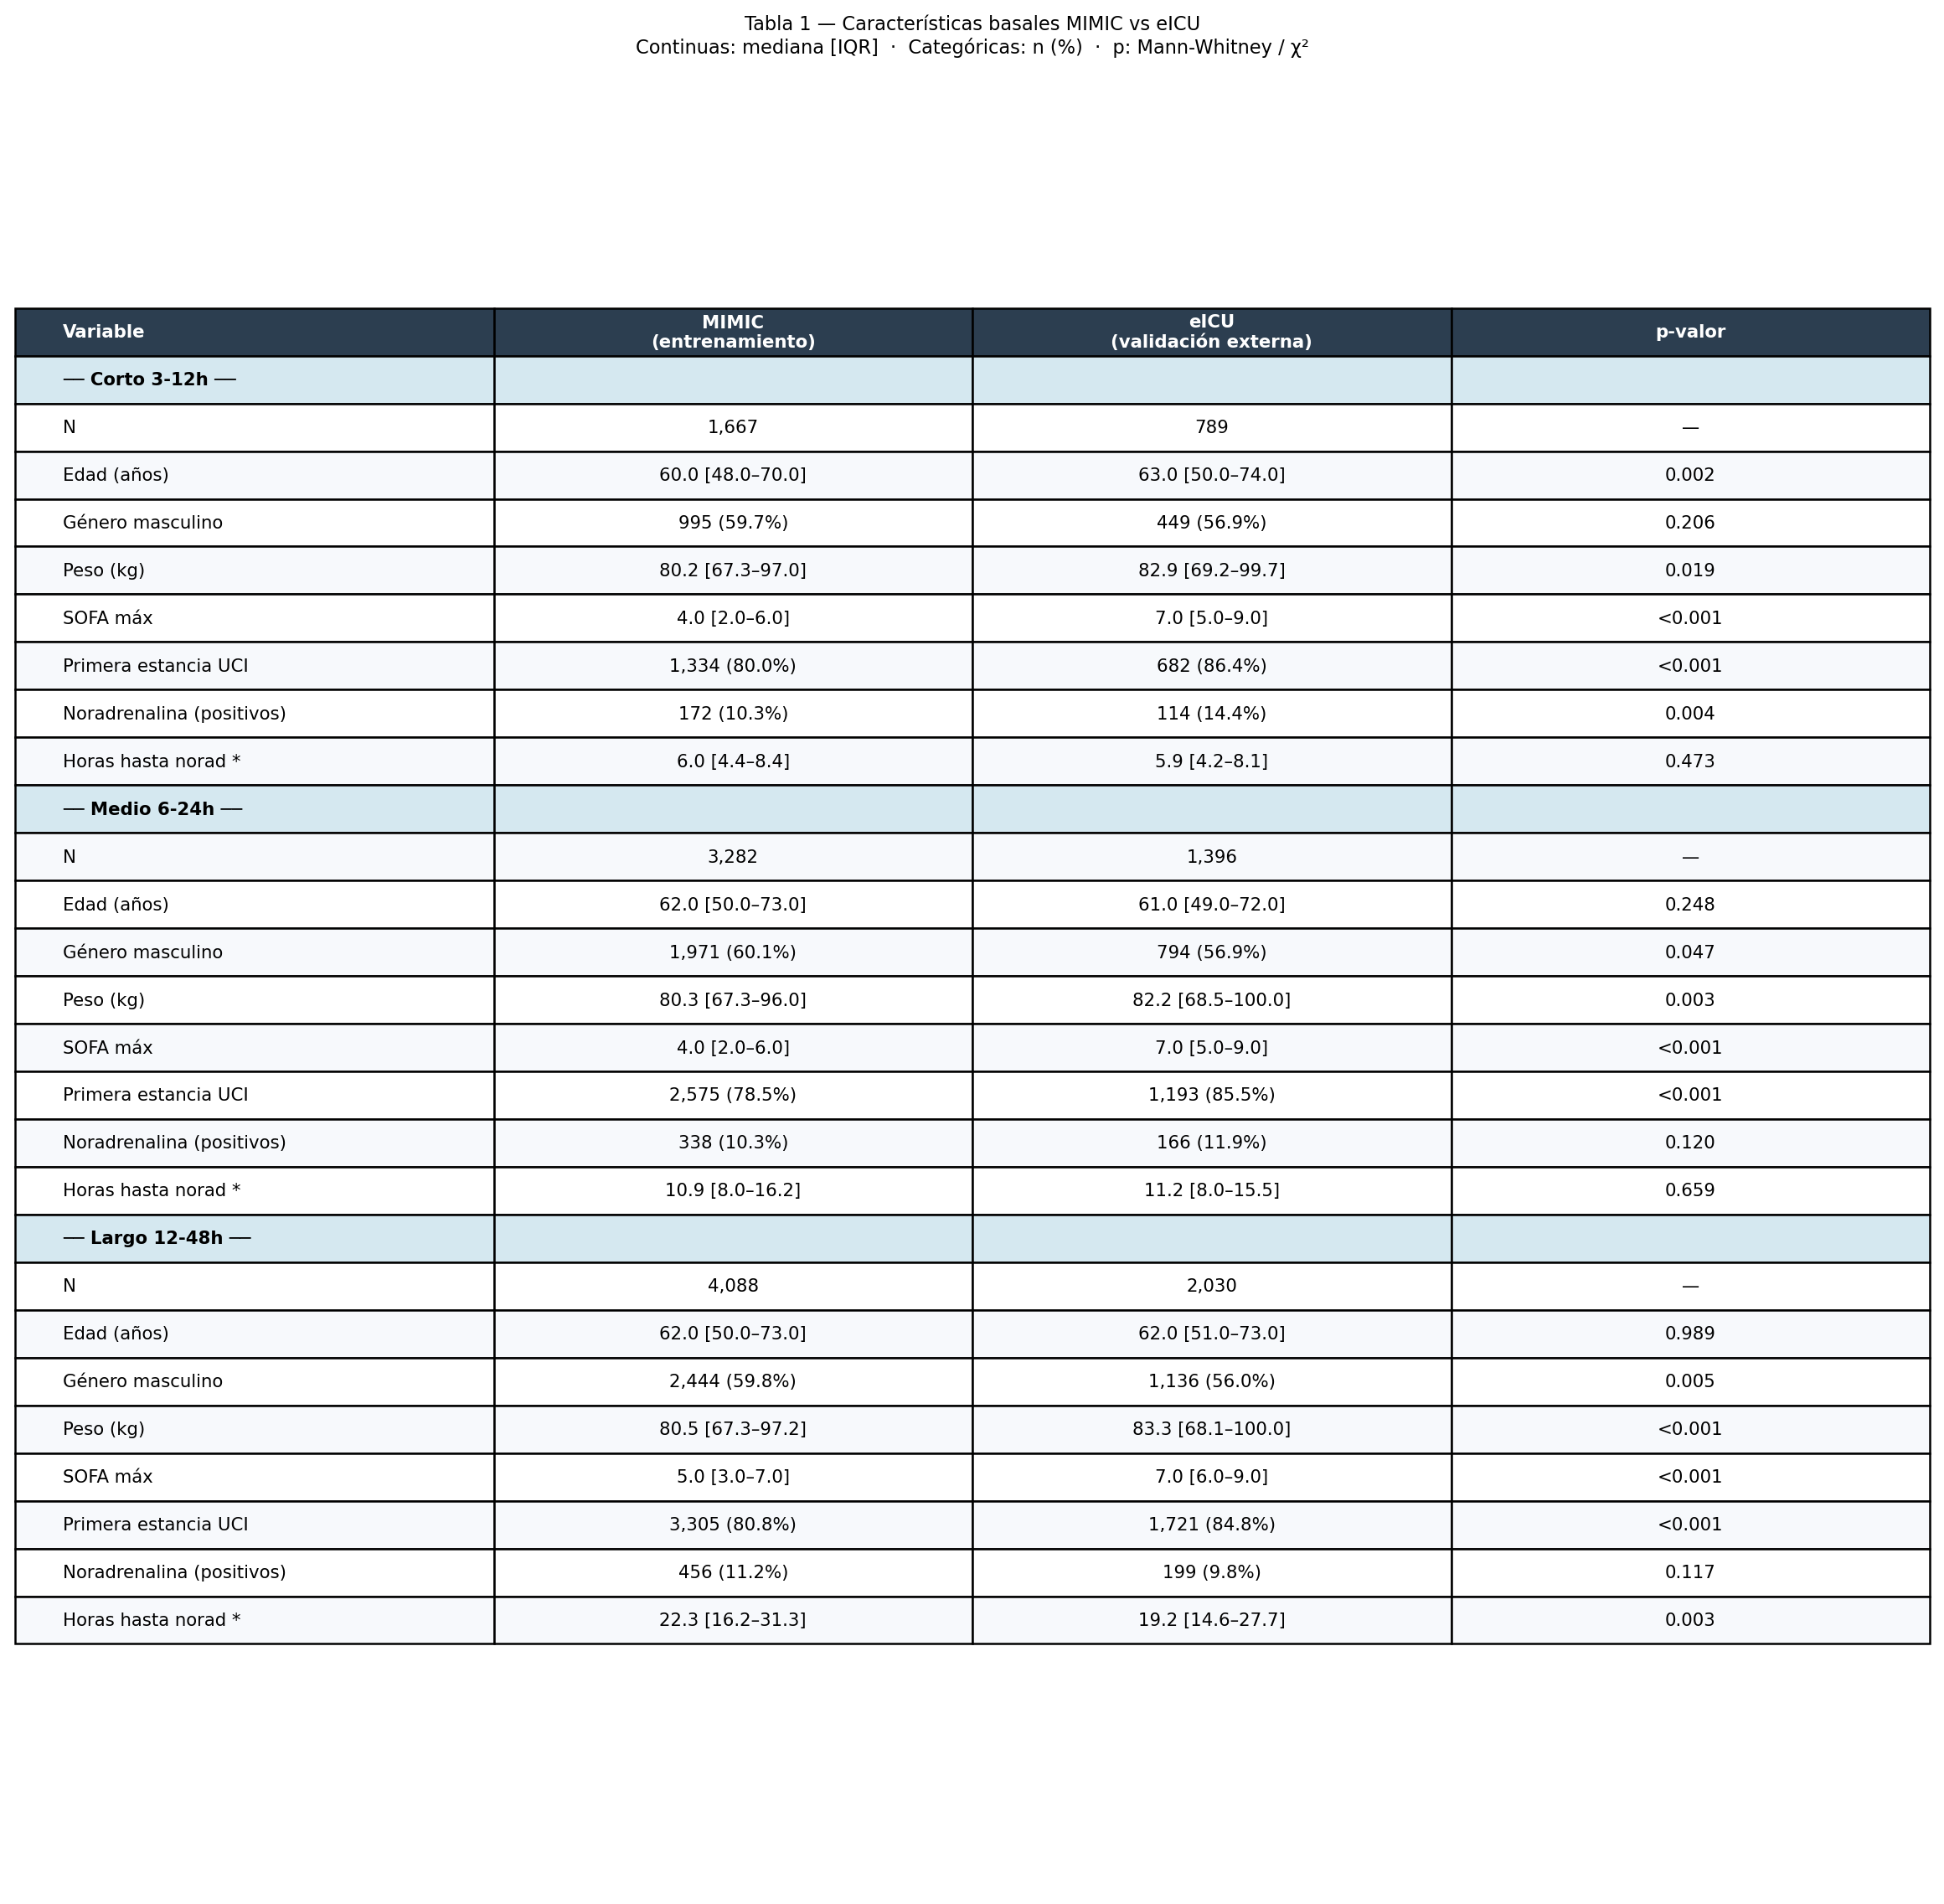
\includegraphics[width=0.92\textwidth]{img/tabla1_mimic_vs_eicu.png}
  \caption{Características basales de las cohortes de MIMIC-IV (desarrollo) y
  eICU-CRD (validación externa) por ventana. Variables continuas como mediana
  [IQR] y categóricas como $n$ (\%), con contraste de Mann-Whitney o $\chi^2$.}
  \label{fig:tabla1}
\end{figure}

%% ══════════════════════════════════════════════════════
%%  APÉNDICE H – Sostenibilización curricular
%% ══════════════════════════════════════════════════════
\apendice{Anexo de sostenibilización curricular}

\section{Reflexión personal sobre sostenibilidad}

La sostenibilidad curricular no puede entenderse únicamente como una cuestión ambiental o de reducción de consumo energético. Siguiendo las directrices de sostenibilidad de la CRUE, 
también implica reflexionar sobre el impacto social, económico, ético y profesional de las decisiones técnicas tomadas durante el desarrollo de un proyecto. En el caso de este TFG, 
esta reflexión resulta especialmente relevante porque el trabajo se sitúa en la intersección entre ingeniería, datos clínicos y cuidados intensivos, un contexto en el que cualquier herramienta 
tecnológica debe diseñarse con prudencia y responsabilidad.

Durante el desarrollo del proyecto he comprendido que un modelo predictivo en salud no puede valorarse solo por sus métricas de rendimiento. Aunque el objetivo técnico era estimar de forma 
temprana el riesgo de inicio de noradrenalina en pacientes de UCI, el objetivo de fondo era explorar si una herramienta de aprendizaje automático podía aportar información útil, interpretable y
 clínicamente revisable. Esta distinción es importante: el sistema no pretende sustituir al médico ni automatizar una decisión terapéutica, sino mostrar una estimación de riesgo acompañada de 
 explicaciones mediante SHAP para facilitar una lectura crítica del resultado. Desde el punto de vista de la sostenibilidad social, esta decisión contribuye a evitar una visión de la inteligencia
  artificial como una caja negra y refuerza el papel del profesional sanitario como responsable final de la interpretación clínica.

El proyecto también me ha permitido desarrollar una competencia clara de contextualización crítica. Trabajar con MIMIC-IV y eICU-CRD ha mostrado que los datos clínicos no son neutros: 
proceden de hospitales concretos, con formas de registro, poblaciones y protocolos propios. Por ello, se incluyó una validación externa sobre eICU-CRD y se evitó presentar el modelo como una 
herramienta universal. Esta limitación no es un defecto menor, sino una parte esencial del aprendizaje: cualquier aplicación futura en un hospital concreto, como el Hospital Universitario de
 Burgos, requeriría validación local, autorización ética y evaluación prospectiva antes de plantear un uso asistencial real.

Desde el punto de vista económico, el trabajo se relaciona con la gestión eficiente de recursos sanitarios críticos. La noradrenalina se utiliza en pacientes con inestabilidad hemodinámica, y
 anticipar el deterioro podría ayudar, en un futuro validado, a planificar mejor la vigilancia, la disponibilidad de personal, las camas de UCI y los recursos terapéuticos. Sin embargo, he 
 intentado no plantear esta posible utilidad como un ahorro demostrado, sino como una línea potencial que todavía necesitaría validación. Esta cautela forma parte de la sostenibilidad
  profesional: no sobreprometer resultados es tan importante como desarrollar modelos técnicamente correctos.

En cuanto al impacto ambiental, el proyecto no se basó en redes neuronales profundas ni en entrenamientos masivos, sino en modelos tabulares relativamente eficientes, como XGBoost, CatBoost,
 Random Forest, regresión logística, Naive Bayes y LightGBM. Aun así, la validación cruzada anidada, la búsqueda de hiperparámetros y el análisis SHAP implicaron un coste computacional no
  despreciable. Esta experiencia me ha hecho más consciente de que la reproducibilidad y el rigor metodológico deben equilibrarse con un uso razonable de recursos. En este sentido, organizar los
 experimentos, conservar los resultados intermedios y evitar ejecuciones innecesarias también forma parte de una práctica sostenible de la ingeniería.

Otra competencia transversal desarrollada ha sido la participación en procesos comunitarios. Aunque el sistema no se validó clínicamente, sí se presentó como prototipo a facultativos de 
Medicina Intensiva del HUBU mediante una encuesta exploratoria. Sus respuestas permitieron valorar la comprensión de la interfaz, la utilidad potencial percibida y la claridad de las 
explicaciones. Esta interacción me ayudó a entender que el diseño de herramientas sanitarias no puede hacerse únicamente desde el código o desde las métricas: necesita incorporar la perspectiva 
de quienes conocen el entorno real de uso.

Finalmente, este TFG ha reforzado mi responsabilidad ética como futuro ingeniero de la salud. Se han respetado las restricciones de uso de MIMIC-IV y eICU-CRD, sin redistribuir datos clínicos 
originales, y se ha mantenido el código en un repositorio público para favorecer la trazabilidad y la revisión. También se ha insistido de forma explícita en que el dashboard es un prototipo 
académico, no una herramienta clínica validada. Para mí, esta es una de las principales lecciones de sostenibilidad del proyecto: desarrollar tecnología sanitaria útil no consiste solo en 
conseguir buenos resultados, sino en reconocer sus límites, documentarlos con honestidad y diseñar siempre pensando en la seguridad del paciente, la transparencia y el uso responsable de los
 recursos.

%% ══════════════════════════════════════════════════════
%%  APÉNDICE I – Registro de interacciones con sistemas de IA
%% ══════════════════════════════════════════════════════

\apendice{Registro de interacciones con sistemas de IA}

\section{Registro de interacciones}

NOTA: la herramienta usada siempre ha sido el modelo Sonnet 4.6 de Claude by Anthropic, a continuación se muestran las interacciones más significativas:

{\small\setlength{\tabcolsep}{4pt}
\begin{longtable*}{@{} p{0.04\linewidth} p{0.14\linewidth} p{0.60\linewidth} p{0.16\linewidth} @{}}
\toprule
\textbf{N.\textsuperscript{o}} & \textbf{Fecha} & \textbf{Prompt / consulta} & \textbf{Uso posterior} \\
\midrule
\endfirsthead
\toprule
\textbf{N.\textsuperscript{o}} & \textbf{Fecha} & \textbf{Prompt / consulta} & \textbf{Uso posterior} \\
\midrule
\endhead
\midrule
\multicolumn{4}{r}{\footnotesize\itshape continúa en la página siguiente}\\
\endfoot
\bottomrule
\endlastfoot
1 & Marzo (1.\textsuperscript{a} q.) & ¿Por qué la noradrenalina se llama norepinefrina en EE.UU. y otros países? & Consulta conceptual \\
\addlinespace
2 & Marzo (2.\textsuperscript{a} q.) & Revisa esta expresión CASE WHEN en SQL para transformar temperaturas de MIMIC-IV de Fahrenheit a Celsius cuando aparecen mezcladas. & Revisión de código SQL \\
\addlinespace
3 & Marzo (2.\textsuperscript{a} q.) & Revisa una consulta SQL de eICU que combina vitalPeriodic y vitalAperiodic para obtener la PAM mínima en una ventana 0--X horas. & Revisión de extracción SQL \\
\addlinespace
4 & Marzo (2.\textsuperscript{a} q.) & Comprueba si la lógica de diuresis deja NULL en pacientes sin registros de orina y solo calcula mL/kg cuando hay volumen y peso válidos. & Control de calidad de datos \\
\addlinespace
5 & Marzo (2.\textsuperscript{a} q.) & Revisa que el SOFA se calcule usando únicamente filas cuyo endtime cae dentro de la ventana de observación, sin imputarlo a cero si no hay registro. & Prevención de sesgo en variables \\
\addlinespace
6 & Marzo (2.\textsuperscript{a} q.) & Qué columnas auxiliares conviene revisar para comprobar que bilirrubina, plaquetas, creatinina, PaO2, FiO2 y GCS están realmente medidos antes del filtrado. & Auditoría de completitud \\
\addlinespace
7 & Abril (1.\textsuperscript{a} q.) & Revisa una función de control previo que comprueba valores perdidos, infinitos y tipos de datos antes de entrenar los modelos. & Preprocesamiento \\
\addlinespace
8 & Abril (1.\textsuperscript{a} q.) & Ayúdame a estructurar una comparación entre el dataset completo y el dataset limpio: pacientes, positivos, prevalencia y variables eliminadas. & Auditoría de datos \\
\addlinespace
9 & Abril (2.\textsuperscript{a} q.) & Revisa una propuesta de organización de la configuración de ventanas Corto\_3\_12, Medio\_6\_24 y Largo\_12\_48 para no duplicar rutas y variables en varios scripts. & Organización del código \\
\addlinespace
10 & Abril (2.\textsuperscript{a} q.) & Comprueba cómo verificar que ningún subject\_id aparezca simultáneamente en train y test dentro de cada fold externo. & Prevención de fuga de pacientes \\
\addlinespace
11 & Abril (2.\textsuperscript{a} q.) & Revisa una función común para calcular AUC-ROC, AUC-PR, Brier, BSS, ECE, sensibilidad, especificidad y F1 de forma homogénea. & Métricas homogéneas \\
\addlinespace
12 & Abril (2.\textsuperscript{a} q.) & Comprueba que el umbral óptimo se elige en train y se evalúa en test sin recalcularlo con datos de test. & Umbral sin fuga de información \\
\addlinespace
13 & Abril (2.\textsuperscript{a} q.) & Revisa el planteamiento de un sistema de checkpoint para leer el CSV de resultados y omitir combinaciones ventana-modelo ya evaluadas. & Reanudación de experimentos \\
\addlinespace
14 & Abril (2.\textsuperscript{a} q.) & Revisa la comparación entre Platt sin regularización, Platt regularizado e isotónico para detectar posibles errores metodológicos o de fuga. & Revisión de calibración \\
\addlinespace
15 & Abril (2.\textsuperscript{a} q.) & Comprueba si el criterio de escoger el menor ECE solo entre calibradores con BSS positivo es coherente y cómo documentarlo. & Selección de calibrador \\
\addlinespace
16 & Abril (2.\textsuperscript{a} q.) & Revisa la fórmula del Brier Skill Score comparando el Brier del modelo frente a una predicción nula basada en la prevalencia. & Métrica de calibración \\
\addlinespace
17 & Abril (2.\textsuperscript{a} q.) & Revisa si el calibrador isotónico puede sobreajustar con pocos positivos y cómo compararlo con Platt usando ECE, BSS y curvas de calibración. & Control metodológico \\
\addlinespace
18 & Abril (2.\textsuperscript{a} q.) & Comprueba cómo calcular pendiente e intercepto de calibración mediante regresión logística sobre el logit de las probabilidades predichas. & Evaluación de calibración \\
\addlinespace
19 & Abril (2.\textsuperscript{a} q.) & Revisa el uso de TreeExplainer para modelos de árboles, manteniendo las variables originales sin escalar. & Revisión de SHAP \\
\addlinespace
20 & Abril (2.\textsuperscript{a} q.) & Revisa cómo aplicar LinearExplainer a la regresión logística cuando los datos han pasado por el escalador del pipeline. & Revisión de SHAP \\
\addlinespace
21 & Abril (2.\textsuperscript{a} q.) & Revisa el planteamiento de KernelExplainer para Naive Bayes con un fondo estratificado que incluya positivos y negativos. & Revisión de SHAP \\
\addlinespace
22 & Abril (2.\textsuperscript{a} q.) & Ayúdame a comprobar una función calcular\_shap que decide entre TreeExplainer, LinearExplainer y KernelExplainer según el algoritmo. & Depuración de SHAP \\
\addlinespace
23 & Abril (2.\textsuperscript{a} q.) & Revisa un script que recorre ventanas y modelos para cargar cada modelo guardado y guardar los gráficos SHAP globales correspondientes. & Automatización de análisis \\
\addlinespace
24 & Abril (2.\textsuperscript{a} q.) & Revisa una forma de resumir importancias SHAP ya calculadas en una tabla o visualización comparativa por variable, algoritmo y ventana. & Comparativa de explicabilidad \\
\addlinespace
25 & Mayo (1.\textsuperscript{a} q.) & Cómo estructurar un wrapper de modelo calibrado compatible con predict\_proba sin romper la integración con sklearn. & Revisión de diseño software \\
\addlinespace
26 & Mayo (1.\textsuperscript{a} q.) & Revisa cómo evitar duplicar la clase del wrapper calibrado entre entrenamiento y dashboard. & Refactorización \\
\addlinespace
27 & Mayo (1.\textsuperscript{a} q.) & Qué metadatos conviene guardar junto al modelo final: variables, calibrador, métricas, ventana y configuración. & Trazabilidad del modelo \\
\addlinespace
28 & Mayo (1.\textsuperscript{a} q.) & Comprueba si es correcto explicar con SHAP el modelo base y usar el calibrador solo para transformar la probabilidad final. & Claridad metodológica \\
\addlinespace
29 & Mayo (1.\textsuperscript{a} q.) & Revisa el esquema para aplicar en eICU un modelo entrenado en MIMIC-IV sin reentrenamiento y detectar incompatibilidades de variables. & Validación externa \\
\addlinespace
30 & Mayo (1.\textsuperscript{a} q.) & Ayúdame a revisar el cálculo de AUC, AUC-PR, Brier, ECE y calibración-in-the-large en la validación externa. & Métricas externas \\
\addlinespace
31 & Mayo (1.\textsuperscript{a} q.) & Cómo presentar una comparación entre rendimiento interno en MIMIC-IV y rendimiento externo en eICU-CRD usando diferencias absolutas de métricas. & Comparación interna-externa \\
\addlinespace
32 & Mayo (1.\textsuperscript{a} q.) & Revisa una función que detecta si el modelo cargado es un Pipeline y extrae por separado el escalador y el estimador final antes de calcular SHAP. & Depuración de pipeline \\
\addlinespace
33 & Mayo (1.\textsuperscript{a} q.) & Revisa qué comprobaciones de forma conviene incluir para verificar que los datos, los valores SHAP y los nombres de variables tienen dimensiones compatibles antes de graficar. & Depuración SHAP \\
\addlinespace
34 & Mayo (1.\textsuperscript{a} q.) & Antes de validar en eICU, comprueba que las variables disponibles coinciden exactamente con las variables del modelo entrenado en MIMIC-IV. & Preparación de validación externa \\
\addlinespace
35 & Mayo (1.\textsuperscript{a} q.) & Imprime por fold el número de pacientes únicos, estancias, positivos, negativos y prevalencia para auditar la validación cruzada. & Auditoría de particiones \\
\addlinespace
36 & Mayo (2.\textsuperscript{a} q.) & Revisa el cálculo de pf\_min en el dashboard a partir de PaO2 y FiO2, evitando divisiones inválidas, infinitos o escalas ambiguas de FiO2. & Ingeniería de variables \\
\addlinespace
37 & Mayo (2.\textsuperscript{a} q.) & Comprueba cómo usar los percentiles de riesgo guardados del entrenamiento para posicionar a pacientes nuevos en Streamlit. & Percentiles en dashboard \\
\addlinespace
38 & Mayo (2.\textsuperscript{a} q.) & Revisa el diseño de una visualización local con percentil de riesgo, datos básicos del paciente y gráfico horizontal de contribuciones SHAP. & Visualización del dashboard \\
\addlinespace
39 & Mayo (2.\textsuperscript{a} q.) & Traduce nombres técnicos de variables a etiquetas clínicas y unidades; por ejemplo, pf\_min como peor PaO2/FiO2. & Lectura clínica \\
\addlinespace
40 & Mayo (2.\textsuperscript{a} q.) & Revisa textos explicativos para aclarar que el percentil es riesgo relativo frente a la cohorte de referencia y no una probabilidad clínica directa. & Explicabilidad \\
\addlinespace
41 & Mayo (2.\textsuperscript{a} q.) & Revisa cómo podría plantearse una validación previa del CSV del paciente, incluyendo columnas obligatorias, tipos numéricos, escala de FiO2 y valores plausibles antes de aplicar el modelo. & Mejora futura del dashboard \\
\addlinespace
42 & Mayo (2.\textsuperscript{a} q.) & Revisa la coherencia de tres CSV ficticios de demostración para comprobar que representan perfiles esperados de bajo, medio y alto riesgo relativo. & Pruebas del dashboard \\
\addlinespace
43 & Mayo (2.\textsuperscript{a} q.) & Revisa cómo cambiar rutas absolutas de Windows a rutas relativas basadas en BASE\_DIR para mejorar la portabilidad del repositorio. & Portabilidad \\
\addlinespace
44 & Mayo (2.\textsuperscript{a} q.) & Revisa la transformación de resultados ya calculados en una tabla de hiperparámetros finales para XGBoost, LightGBM, Random Forest, CatBoost, regresión logística y Naive Bayes. & Documentación de entrenamiento \\
\addlinespace
45 & Mayo (2.\textsuperscript{a} q.) & Revisa la transformación de resultados estadísticos ya obtenidos en una tabla resumen de variables significativas por regresor. & Resultados \\
\addlinespace
46 & Mayo (2.\textsuperscript{a} q.) & Revisa una nota de documentación en el código para aclarar que los valores SHAP pertenecen al modelo base y que la calibración solo transforma la probabilidad final. & Claridad metodológica \\
\addlinespace
47 & Mayo (2.\textsuperscript{a} q.) & Revisa un texto bajo el gráfico SHAP que aclare que las barras indican contribución al modelo, no causalidad clínica. & Advertencia metodológica \\
\end{longtable*}
}


\backmatter
\bibliography{bibliografiaAnexos.bib}



\end{document}
